\documentclass{article}
\usepackage[usenames,dvipsnames]{color}
\usepackage[utf8]{inputenc}
\usepackage{lscape}
\usepackage[colorlinks = true,
            linkcolor = blue,
            urlcolor  = blue,
            citecolor = blue,
            anchorcolor = blue]{hyperref}
\usepackage{amsmath}
\hypersetup{
    colorlinks=true,
    linkcolor=blue,
    filecolor=magenta,      
    urlcolor=blue,
}
\usepackage{tikz}
\newcommand{\roundpic}[4][]{
  \tikz\node [circle, minimum width = #2,
    path picture = {
      \node [#1] at (path picture bounding box.center) {
        \includegraphics[width=#3]{#4}};
    }] {};}
    
\usepackage{indentfirst}
\usepackage[a4paper,margin={1.2in,1.5in},vmargin={1.2in,1.5in}]{geometry}
\geometry{paperwidth=210mm,paperheight=297mm,
textwidth=150mm,textheight=210mm,
top=23mm,bottom=23mm,
left=23mm,right=23mm}
\usepackage[colorlinks,linkcolor=blue,hyperindex]{hyperref}
\usepackage[brazil]{babel}
\usepackage{graphicx,color,wrapfig}
\usepackage{multicol}
%\usetikzlibrary{mindmap}
%\pagestyle{empty}
\usepackage{fancyhdr}
\pagestyle{fancy}
\fancyhead[]{}
\rhead{\textit{\faRProject para estudantes de marketing}}
\lhead{\thepage}
\fancyfoot[]{}
\renewcommand{\headrulewidth}{0.1pt}
\usepackage{color,soul}
\usepackage{color}
\usepackage{listings}%pacote para literalizar os códigos do R no Latex
\usepackage{xcolor}

\usepackage[dvipsnames]{xcolor}

\definecolor{mygray}{gray}{0.95}

\definecolor{codegreen}{rgb}{0,0.4,0}
\definecolor{codegray}{rgb}{0.5,0.5,0.5}
\definecolor{codepurple}{rgb}{0.38,0,0.82}
\definecolor{backcolour}{rgb}{0.95,0.95,0.92}

\lstdefinestyle{mystyle}{
    backgroundcolor=\color{mygray},   
    commentstyle=\color{codegreen},
    keywordstyle=\color{blue},
    numberstyle=\tiny\color{codegray},
    stringstyle=\color{codepurple},
    basicstyle=\ttfamily\footnotesize,
    breakatwhitespace=false,         
    breaklines=true,                 
    captionpos=b,                    
    keepspaces=true,                 
   % numbers=left,                    
    numbersep=5pt,                  
    showspaces=false,                
    showstringspaces=false,
    showtabs=false,                  
    tabsize=2
}

\lstset{style=mystyle}
%=========fim da instrução do listings
\usepackage{xcolor}
\usepackage[fixed]{fontawesome5}
\usepackage{tcolorbox}
\usepackage{comment}

\usepackage[framemethod=TikZ]{mdframed}
\mdfdefinestyle{MyFrame}{%
    linecolor=blue,
    outerlinewidth=1pt,
    roundcorner=40pt,
    innertopmargin=\baselineskip,
    innerbottommargin=\baselineskip,
    innerrightmargin=10pt,
    innerleftmargin=10pt,
    backgroundcolor=gray!50!white}
%============================================================
%========================================================
\begin{document}


%============================================================

\title{\faRProject~para estudantes de marketing \\\textit{KU Leuven Marketing department}}
\author{\href{https://rhozon.github.io/}{Traduzido por Rodrigo Hermont Ozon\footnote{Economista e Mestre em Desenvolvimento Econômico pela UFPR.}}}
\date{Maio, 2020}

\maketitle



\thispagestyle{empty}
%===========================================================
\newpage

\begin{mdframed}[style=MyFrame]

\fbox{%
\roundpic[xshift=-.00000095cm,yshift=-.0006cm]{3.8cm}{3cm}{me.jpg}%
}


\section*{Sobre o autor desta tradução:}


\textit{Rodrigo Hermont Ozon, economista e apaixonado por econometria, pelas aplicações de modelos econômicos a problemas reais e cotidianos vivenciados na sociedade e na realidade do mundo empresarial e corporativo.}


\begin{flushleft}
Seus contatos podem ser acessados em:

\begin{itemize}
\item \href{https://rhozon.github.io/}{\faGithub} \href{https://rhozon.github.io/}{Github}

\item \href{https://www.linkedin.com/in/rodrigohermontozon/}{\faLinkedin} \href{https://www.linkedin.com/in/rodrigohermontozon/}{Linkedin} %
\end{itemize}
\end{flushleft}


\end{mdframed}

\vspace{9cm}


\begin{abstract}
  O objetivo de traduzir esse tutorial consiste em facilitar o aprendizado e utilização da linguagem estatística \faRProject para os profissionais de marketing e demais áreas de negócio que precisam se adequar a uma realidade mutante e movida por um fluxo significativo de informações por todos os lados. Trabalhar e interpretar bem os dados é um desafio computacional para muitos profissionais dessa área; e esta tradução visa cobrir (ainda que superficialmente) tal lacuna.
  Este e-book foi escrito no \href{http://www.overleaf.com}{overleaf} com o pacote knitr \href{https://bookdown.org/content/1340/}{para a página interativa de autoria de KU Leven Marketing Department.}
\end{abstract}


\thispagestyle{empty}
%==============================================================
\newpage

.

\vspace{22cm}
Ao meu amado paizão e professor pra vida inteira, Ronaldo --  \textit{"Ensina a criança no caminho em que deve andar, e, ainda quando for velho, não se desviará dele."}

\vspace{.15cm}
\hspace{13cm}\href{https://bibliaportugues.com/proverbs/22-6.htm}{Provérbios 22:6}

\thispagestyle{empty}

%==========================================================

\newpage
\tableofcontents
%\lstlistoflistings



%\hspace{12cm}\includegraphics[widht=1.5cm,height=1.5cm]{erasmussign.png}
\thispagestyle{headings}

\newpage
%====================================================
\section*{Nota do tradutor}
.

\vspace{5cm}
Esse e-book traduzido é oriundo de \fbox{\textit{\href{https://bookdown.org/content/1340/}{\faRProject for marketing students}}.}

\vspace{.25cm}
\href{https://static1.squarespace.com/static/5757268f7da24f26ca7b21d2/t/5c7587114192021796d7cc84/1551206162093/R_Overleaf_Integration.pdf}{Para que os scripts funcionem corretamente recomendo que você faça a integração do seu \faRProject Studio com o Overleaf observando \fbox{esse tutorial aqui}.}

\vspace{.25cm}
\textit{*As traduções aqui são somente as transcrições. Não me preocupei em aperfeiçoá-las para a língua portuguesa com maior nível de clareza nos textos. As figuras e imagens não foram traduzidas.}

\newpage

\section{Sobre esse tutorial}


Neste tutorial, exploraremos o \faRProject como uma ferramenta para analisar e visualizar dados.\faRProject é uma linguagem de programação estatística que rapidamente ganhou popularidade em muitos campos científicos. A principal diferença entre o \faRProject e outro software estatístico como o SPSS é que o \faRProject não possui interface gráfica com o usuário. Não há botões para clicar. \faRProject é executado inteiramente digitando comandos em uma interface de texto. Isso pode parecer assustador, mas, esperançosamente, no final deste tutorial, você verá como o \faRProject pode ajudá-lo a fazer uma melhor análise estatística.

Então, por que estamos usando \faRProject e não um dos muitos outros pacotes estatísticos como SPSS, SAS ou Microsoft Excel? Algumas das razões mais importantes:

Ao contrário de outros softwares, o \faRProject é gratuito e de código aberto, e sempre será!
\faRProject é uma linguagem de programação e não uma interface gráfica como o SPSS. Ele realiza análises ou visualizações executando algumas linhas de código. Essas linhas de código podem ser salvas como scripts para repetição futura das análises ou visualizações. Também facilita o compartilhamento de seu trabalho com outras pessoas, que podem aprender ou corrigi-lo se houver algum erro.

\faRProject tem uma comunidade online muito ativa e útil. Quando você se depara com um problema, muitas vezes basta uma rápida pesquisa no Google para encontrar uma solução de origem coletiva.


Todas as principais empresas de pesquisa de marketing indicam que estão experimentando o \faRProject e que o \faRProject é o software do futuro.
Este tutorial se concentra em análises estatísticas relevantes para estudantes de marketing. Se você quiser uma introdução mais extensa, porém acessível, ao \faRProject, confira o excelente e gratuito livro "\href{http://r4ds.had.co.nz/index.html}{R for Data Science}". Este capítulo introdutório e o próximo são baseados na introdução ao R1, encontrada nos tutoriais do \href{https://ourcodingclub.github.io/}{Coding Club}, que também possui muitos outros ótimos tutoriais de \faRProject.

Este tutorial foi escrito no RMarkdown, com a ajuda do incrível \href{https://bookdown.org/yihui/bookdown/}{pacote \fbox{bookdown}.}

Questões? Comentários? Sugestões? Envie-me um e-mail: \href{mailto:samuel.franssens@kuleuven.be}{samuel.franssens@kuleuven.be}

\subsection{Download e instalação do \faRProject e \faRProject Studio}

Para fornecer algumas funcionalidades extras e facilitar um pouco a transição, usaremos um programa chamado \faRProject Studio como um front-end gráfico para \faRProject.

Você pode fazer o download do \faRProject em \href{https://cloud.r-project.org/}{https://cloud.r-project.org/}. Selecione o link apropriado para o seu sistema operacional e instale o \faRProject no seu computador (no Windows, você primeiro precisa clicar em "base").

Em seguida, faça o download do \faRProject Studio em \href{https://www.rstudio.com/products/rstudio/download/}{https://www.rstudio.com/products/rstudio/download/}. Selecione o instalador para a versão gratuita e instale o \faRProject Studio (nota: você precisa ter o \faRProject instalado primeiro).

\subsection{Obtendo familiaridade com o \faRProject Studio}
\subsubsection{Console vs. script}

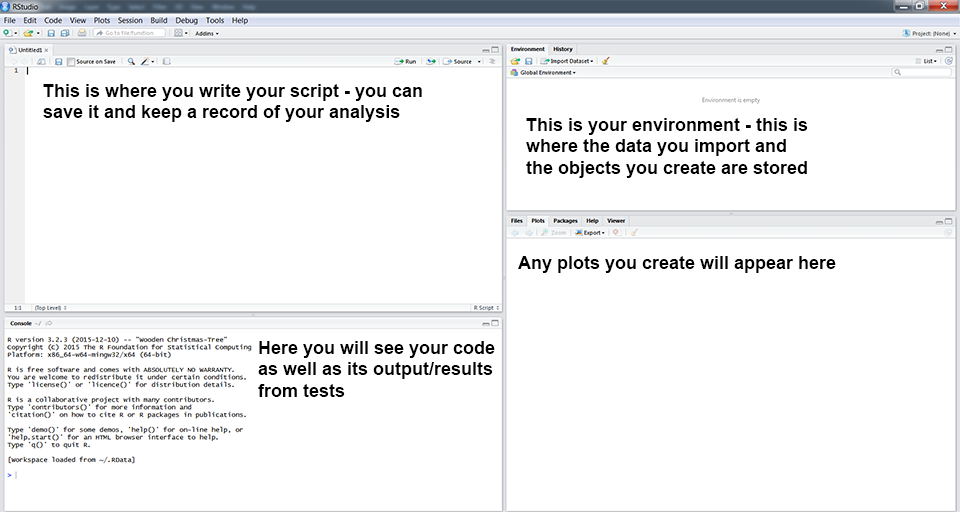
\includegraphics[widht=8cm,height=8cm]{rstudio.png}

Ao abrir o \faRProject Studio, você verá uma janela como a acima. Você pode digitar o código diretamente no console (janela inferior esquerda) - basta digitar seu código após o prompt ($>$) e pressionar enter no final da linha para executar o código. Você também pode escrever seu código no arquivo de script (a janela superior esquerda). Se você não ver uma janela com um arquivo de script, abra uma clicando em Arquivo, Novo arquivo, \faRProject Script. Para executar uma linha de código a partir do seu script, pressione Ctrl + R ou Ctrl + Enter no Windows e Cmd + Enter no Mac ou use o botão 'Executar' no canto superior direito da janela do script.

O código digitado diretamente no console não será salvo pelo \faRProject. O código digitado em um arquivo de script pode ser salvo como um registro reproduzível de sua análise. Se você estiver trabalhando no console e quiser editar ou executar novamente uma linha de código anterior, pressione a seta para cima. Se você estiver trabalhando em um script, lembre-se de clicar em Salvar frequentemente (Arquivo, Salvar), para que você realmente salve o seu script!

É melhor trabalhar em arquivos de script. Também é altamente recomendável salvar seu arquivo de script em uma pasta que é automaticamente copiada pelo software de compartilhamento de arquivos que oferece a funcionalidade "versões anteriores" (o \href{https://www.dropbox.com/business/landing-t61fl-v2?_tk=paid_sem_goog_biz_b&_camp=1411326950&_kw=dropbox|e&_ad=389658655593||c&gclid=CjwKCAjwtqj2BRBYEiwAqfzur1JwrYwkXrKtxYHo_nfrnCMIUBe-IpmrIgCZmTt0l3gibHmKgokdvBoChx8QAvD_BwE}{Dropbox} é provavelmente o mais famoso; aqui estão algumas \href{https://medium.com/@Vanina/dropbox-alternatives-top-5best-cloud-storage-services-2017-a703af7d7796}{alternativas}). Isso lhe dará a opção de restaurar versões salvas anteriormente de seus arquivos sempre que você salvar algo por engano. Como qualquer peça escrita, os roteiros se beneficiam de estrutura e clareza - a \href{https://ourcodingclub.github.io/2017/04/25/etiquette.html}{Coding Etiquette do Coding Club} oferece mais conselhos sobre isso.

\subsubsection{Comentários}

Ao escrever um script, é muito importante adicionar comentários para descrever o que você está fazendo e por quê. Você pode fazer isso inserindo um # na frente de uma linha de texto. Comece seu script gravando quem está escrevendo o roteiro, a data e o objetivo principal - no capítulo introdutório, aprenderemos sobre as acomodações do Airbnb na Bélgica. Aqui está um exemplo:

\begin{lstlisting}[language=R]
# Aprendendo a importar e explorar dados e criar graficos investigando as acomodacoes do Airbnb na Belgica
# Escrito por Samuel Franssens 28/01/2018
\end{lstlisting}

\subsubsection{Pacotes}

As próximas linhas de código geralmente carregam os pacotes que você usará em sua análise ou visualização. 

O \faRProject carrega automaticamente várias funções para executar operações básicas, mas os pacotes fornecem funcionalidade extra. Eles geralmente consistem em várias funções que podem lidar com tarefas específicas. Por exemplo, um pacote poderia fornecer funções para fazer análises de cluster ou para fazer biplots. Para instalar um pacote, digite install.packages ("nome do pacote") (e pressione enter ao trabalhar no console ou pressione Ctrl + Enter, Ctrl + R, Cmd + Enter ou o botão 'Executar' ao trabalhar em um script).

Você só precisa instalar pacotes uma vez; depois, basta carregá-los usando a biblioteca (nome do pacote). Aqui, usaremos o popular pacote tidyverse que fornece muitas funções úteis e intuitivas

 (\href{https://www.tidyverse.org/}{https://www.tidyverse.org/}).
 
O pacote tidyverse é na verdade uma coleção de outros pacotes; portanto, durante a instalação ou o carregamento, você verá que vários pacotes são instalados ou carregados. Instale e carregue o pacote tidyverse executando as seguintes linhas de código:

\begin{lstlisting}[language=R]
install.packages("tidyverse") # instala o pacote tidyverse
library(tidyverse) # carrega o pacote tidyverse
\end{lstlisting}

Observe que há aspas ao instalar um pacote, mas não ao carregá-lo.

A instalação de um pacote normalmente produz muita saída no console. Você pode verificar se instalou um pacote com êxito, carregando o pacote. Se você tentar carregar um pacote que não foi instalado com sucesso, você receberá o seguinte erro:
\begin{lstlisting}[language=R]
library(marketing) # Estou tentando instalar o pacote inexistente 'marketing'
\end{lstlisting}

\begin{lstlisting}[language=R]
## Error in library(marketing): there is no package called 'marketing'
\end{lstlisting}


Nesse caso, tente reinstalar o pacote.

Quando você tenta usar uma função de um determinado pacote que ainda não foi carregado, você pode receber o seguinte erro:

\begin{lstlisting}[language=R]
# agnes eh uma funcao do pacote cluster para rodar analise de cluster.
agnes(dist(data), metric = "euclidean", method = "ward")
\end{lstlisting}
\begin{lstlisting}[language=R]
## Error in agnes(dist(data), metric = "euclidean", method = "ward"): could not find function "agnes"
\end{lstlisting}

O \faRProject nos dirá que não pode encontrar a função solicitada (neste caso, agnes, uma função do pacote de cluster para análises de cluster). Geralmente, isso ocorre porque você ainda não carregou (ou instalou) o pacote ao qual a função pertence.

Após instalar e carregar o pacote tidyverse, você poderá usar as funções incluídas no pacote tidyverse. Como você usará o pacote tidyverse com tanta frequência, é melhor sempre carregá-lo no início do seu script.

\section{Introdução ao \faRProject}

Neste capítulo introdutório, você aprenderá:

\begin{itemize}
    \item como importar dados
    \item como manipular um conjunto de dados com o operador de canal
    \item como resumir um conjunto de dados
    \item como fazer gráficos de dispersão e histogramas
\end{itemize}

\subsection{Importando dados}

Neste capítulo, exploraremos um conjunto de dados publicamente disponível dos dados do Airbnb. Encontramos esses dados \href{http://tomslee.net/airbnb-data-collection-get-the-data}{aqui.} (Estes são dados reais “raspados” do airbnb.com em julho de 2017. Isso significa que o proprietário do site criou um script para coletar automaticamente esses dados no site airbnb.com. Essa é uma das muitas coisas que você também pode fazer no \faRProject. Mas primeiro vamos aprender o básico.) Você pode baixar o conjunto de dados clicando com o botão direito do mouse \href{http://users.telenet.be/samuelfranssens/tutorial_data/tomslee_airbnb_belgium_1454_2017-07-14.csv}{neste link}, selecionando “Salvar link como…” (ou algo semelhante) e salvando o arquivo .csv em um diretório no disco rígido. Como mencionado na \href{https://bookdown.org/content/1340/getting-familiar-with-rstudio.html#console_script}{introdução}, é uma boa ideia salvar seu trabalho em um diretório que é automaticamente copiado pelo software de compartilhamento de arquivos. Mais tarde, salvaremos nosso script no mesmo diretório.


\subsubsection{Importando arquivos .csv}

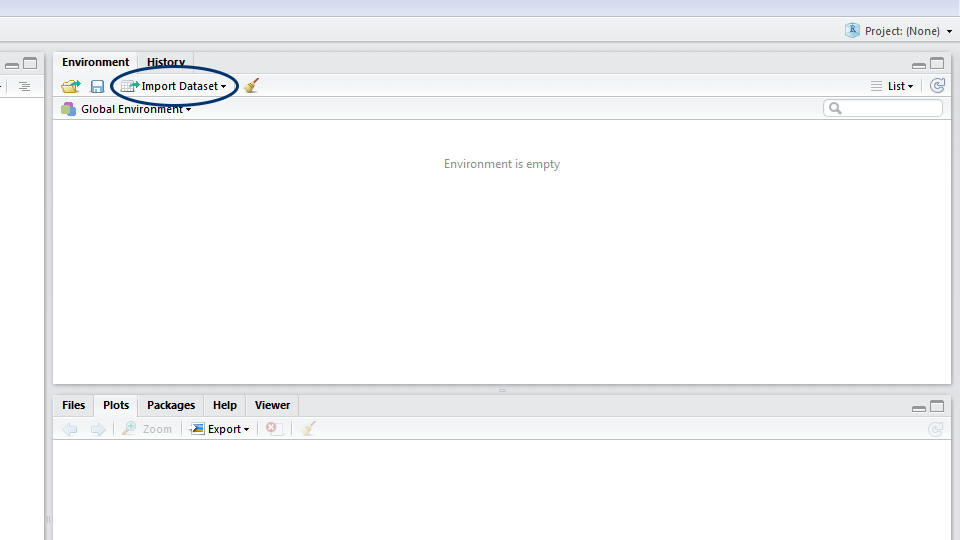
\includegraphics[width=14cm,height=8cm]{rstudio2.png}


Para importar dados para o \faRProject, clique em Import Dataset e depois em From text (readr). Uma nova janela será exibida. Clique em Procurar e encontre seu arquivo de dados. Certifique-se de que Primeira linha como nomes esteja selecionada (isso diz ao \faRProject para tratar a primeira linha dos seus dados como os títulos das colunas) e clique em Importar. Após clicar em importar, o \faRProject Studio abre uma guia Visualizador. Isso mostra seus dados em uma planilha.

Alguns computadores salvam arquivos .csv com ponto e vírgula (;) em vez de vírgulas (,) como separadores ou "delimitadores". Isso geralmente acontece quando o inglês não é o primeiro ou o único idioma do seu computador. Se seus arquivos estiverem separados por ponto e vírgula, clique em Importar conjunto de dados e encontre seu arquivo de dados, mas agora escolha Ponto e vírgula no delimitador do menu suspenso.

Nota: se você não salvou o conjunto de dados clicando com o botão direito do mouse no link e selecionando “Salvar link como…”, mas clicou com o botão esquerdo do mouse no link, seu navegador pode ter acabado abrindo o conjunto de dados. Você pode salvar o conjunto de dados pressionando Ctrl + S. Observe, no entanto, que seu navegador pode acabar salvando o conjunto de dados como um arquivo .txt. É importante alterar a extensão do seu arquivo nos argumentos para o comando read\_csv abaixo.

\subsubsection{Ajustando seu diretório de trabalho}

Depois de importar seus dados com Import Dataset, verifique a janela do console. Você verá o comando para abrir o Visualizador (View()) e, uma linha acima, verá o comando que lê os dados. Copie o comando que lê os dados do console para o seu script. No meu caso, fica assim:

\begin{lstlisting}[language=R]
tomslee_airbnb_belgium_1454_2017_07_14 <- read_csv("c:/Dropbox/work/teaching/R/data/tomslee_airbnb_belgium_1454_2017-07-14.csv") 
# Mude .csv para .txt se necessario
\end{lstlisting}

Esta linha tem a seguinte leitura (da direita para a esquerda): a funcao read\_csv deve ler o arquivo tomslee\_airbnb\_belgium\_1454\_2017-07-14.csv no diretorio c: / Dropbox / work / teaching / R / data / (voce vera um diretorio diferente aqui ) Em seguida, R deve atribuir ($<-$) esses dados a um objeto chamado tomslee\_airbnb\_belgium\_1454\_2017\_07\_14.

Antes de explicar cada um desses conceitos, vamos simplificar esta linha de código:
\begin{lstlisting}[language=R]
setwd("c:/Dropbox/work/teaching/R/data/") # Ajusta o diretorio de trabalho para onde o R precisa apontar para o arquivo .csv
airbnb <- read_csv("tomslee_airbnb_belgium_1454_2017-07-14.csv") 
# read_csv agora nao precisa mais de um diretorio e somente precisa de um nome de arquivo
# Atribuimos os dados a um objeto com um nome mais simples: airbnb em vez de tomslee_airbnb_belgium_1454_2017_07_14
\end{lstlisting}

O comando setwd informa ao \faRProject onde está o seu diretório de trabalho. Seu diretório de trabalho é uma pasta no seu computador onde o \faRProject procurará dados, onde as plotagens serão salvas etc. Defina seu diretório de trabalho na pasta em que os dados foram armazenados. Agora, o arquivo read\_csv não requer mais um diretório.

Você só precisa definir seu diretório de trabalho uma vez, na parte superior do seu script. Você pode verificar se está definido corretamente executando getwd(). Observe que em um computador com Windows, os caminhos de arquivo possuem barras invertidas que separam as pastas \begin{verbatim} ("C: \ folder \ data").\end{verbatim} 

No entanto, o caminho do arquivo digitado no \faRProject deve usar barras ("C: / folder / data").

Salve este script no diretório de trabalho (no meu caso: c: / Dropbox / trabalho / ensino / R / dados /)). No futuro, você pode simplesmente executar essas linhas de código para importar seus dados em vez de clicar em Importar conjunto de dados (a execução de linhas de código é muito mais rápida do que apontar e clicar - uma das vantagens do uso do \faRProject).

Não se esqueça de carregar o pacote tidyverse na parte superior do seu script (mesmo antes de definir o diretório de trabalho) com a biblioteca (tidyverse).


\subsubsection{Atribuindo dados a objetos}

Observe a seta $<-$ no meio da linha que importou o arquivo .csv:

\begin{lstlisting}
airbnb <- read_csv("tomslee_airbnb_belgium_1454_2017-07-14.csv")
\end{lstlisting}

$<-$ é o operador de atribuição. Nesse caso, atribuímos o conjunto de dados (ou seja, os dados que lemos do arquivo .csv) a um objeto chamado airbnb. Um objeto é uma estrutura de dados. Todos os objetos que você criar serão exibidos no painel Ambiente (a janela superior direita). O \faRProject Studio fornece um atalho para escrever $<-$: Alt + - (no Windows). É uma boa ideia aprender esse atalho de cor.

Quando você importa dados para o \faRProject, ele se torna um objeto chamado quadro de dados. Um quadro de dados é como uma tabela ou uma planilha do Excel. Tem duas dimensões: linhas e colunas. Geralmente, as linhas representam suas observações, as colunas representam as diferentes variáveis. Quando seus dados consistem em apenas uma dimensão (por exemplo, uma sequência de números ou palavras), eles são armazenados em um segundo tipo de objeto chamado vetor. Mais tarde, aprenderemos como criar vetores.

\newpage
\subsubsection{Importando arquivos do Excel}

\faRProject funciona melhor com arquivos .csv (valores separados por vírgula). No entanto, os dados geralmente são armazenados como um arquivo do Excel (você pode baixar o conjunto de dados do Airbnb como um arquivo do Excel aqui). O \faRProject também pode lidar com isso, mas você precisará carregar primeiro um pacote chamado \fbox{readxl} (este pacote faz parte do pacote \fbox{tidyverse}, mas não é carregado com a biblioteca (\fbox{tidyverse}) porque não é um pacote \fbox{tidyverse} principal):

\begin{lstlisting}[language=R]
library (readxl) # carrega o pacote

airbnb.excel <- read_excel (path = "tomslee_airbnb_belgium_1454_2017-07-14.xlsx", sheet = "Sheet1")
# verifique se o arquivo do Excel está salvo no seu diretório de trabalho

# você também pode deixar de fora o path = & sheet =
# então o comando se torna: read_excel ("tomslee_airbnb_belgium_1454_2017-07-14.xlsx", "Sheet1")
\end{lstlisting}


\fbox{read\_excel} é uma função do pacote \fbox{readxl}. São necessários dois argumentos: o primeiro é o nome do arquivo e o segundo é o nome da planilha do Excel que você deseja ler.

\subsubsection{Lendo os dados do Airbnb}

Nosso conjunto de dados contém informações sobre quartos na Bélgica listados no airbnb.com. Sabemos para cada sala (identificada por \fbox{room\_id}): quem é o hóspede (\fbox{host\_id}), que tipo de sala é (\fbox{room\_type}), onde está localizada (\fbox{country}, \fbox{city}, \fbox{neighborhood} e até a \fbox{latitude} e \fbox{longitude} exata), como muitas críticas que recebeu (\fbox{reviews}), como as pessoas estavam satisfeitas (\fbox{overall\_satisfaction}), preço (\fbox{price}) e características dos quartos (\fbox{accommodates}, \fbox{bedrooms}, \fbox{bathrooms}, \fbox{minstay}).

Uma etapa realmente importante é verificar se seus dados foram importados corretamente. É uma boa prática sempre inspecionar seus dados. Você vê algum valor ausente, os números e os nomes fazem sentido? Se você começar imediatamente com a análise, corre o risco de ter que refazê-la porque os dados não foram lidos corretamente, ou pior, analisando dados errados sem perceber.


\begin{lstlisting}[language=R]
airbnb # Visualiza o conteudo do conjunto de dados da Airbnb

## # A tibble: 17,651 x 20
##    room_id survey_id host_id room_type country city  borough neighborhood
##      <int>     <int>   <int> <chr>     <chr>   <chr> <chr>   <chr>       
##  1  5.14e6      1454  2.07e7 Shared r~ <NA>    Belg~ Gent    Gent        
##  2  1.31e7      1454  4.61e7 Shared r~ <NA>    Belg~ Brussel Schaarbeek  
##  3  8.30e6      1454  3.09e7 Shared r~ <NA>    Belg~ Brussel Elsene      
##  4  1.38e7      1454  8.14e7 Shared r~ <NA>    Belg~ Oosten~ Middelkerke 
##  5  1.83e7      1454  1.43e7 Shared r~ <NA>    Belg~ Brussel Anderlecht  
##  6  1.27e7      1454  6.88e7 Shared r~ <NA>    Belg~ Brussel Koekelberg  
##  7  1.55e7      1454  9.91e7 Shared r~ <NA>    Belg~ Gent    Gent        
##  8  3.91e6      1454  3.69e6 Shared r~ <NA>    Belg~ Brussel Elsene      
##  9  1.49e7      1454  3.06e7 Shared r~ <NA>    Belg~ Vervie~ Baelen      
## 10  8.50e6      1454  4.05e7 Shared r~ <NA>    Belg~ Brussel Etterbeek   
## # ... with 17,641 more rows, and 12 more variables: reviews <int>,
## #   overall_satisfaction <dbl>, accommodates <int>, bedrooms <dbl>,
## #   bathrooms <chr>, price <dbl>, minstay <chr>, name <chr>,
## #   last_modified <dttm>, latitude <dbl>, longitude <dbl>, location <chr>
\end{lstlisting}


O \faRProject nos diz que estamos lidando com uma \fbox{tibble} (essa é apenas outra palavra para quadro de dados) com 17651 linhas ou observações e 20 colunas ou variáveis. Para cada coluna, é fornecido o tipo da variável: int (inteiro), chr (caractere), dbl (duplo), dttm (data e hora). Variáveis inteiras e duplas armazenam números (inteiro para números redondos, duplicam para números com decimais), variáveis de caracteres armazenam letras, variáveis de data e hora armazenam datas e / ou horas.

O \faRProject imprime apenas os dados das dez primeiras linhas e o número máximo de colunas que cabem na tela. Se, no entanto, você deseja inspecionar todo o conjunto de dados, clique duas vezes no objeto airbnb no painel Ambiente (a janela superior direita) para abrir uma aba Visualizador ou executar a Visualização (airbnb). Observe o V maiúsculo no comando Visualizar. O \faRProject sempre diferencia maiúsculas de minúsculas!

Você também pode usar o comando \fbox{print} para solicitar mais (ou menos) linhas e colunas na janela do console:

\begin{lstlisting}[language=R]
# Imprima 25 linhas (defina como Inf para imprimir todas as linhas) e defina a largura como 100 para ver mais colunas.
# Observe que as colunas que nao cabem na primeira tela com 25 linhas
# sao impressos abaixo das 25 linhas iniciais.

print (airbnb, n = 25, width = 100)

## # A tibble: 17,651 x 20
##    room_id survey_id host_id room_type country city  borough neighborhood
##      <int>     <int>   <int> <chr>     <chr>   <chr> <chr>   <chr>       
##  1  5.14e6      1454  2.07e7 Shared r~ <NA>    Belg~ Gent    Gent        
##  2  1.31e7      1454  4.61e7 Shared r~ <NA>    Belg~ Brussel Schaarbeek  
##  3  8.30e6      1454  3.09e7 Shared r~ <NA>    Belg~ Brussel Elsene      
##  4  1.38e7      1454  8.14e7 Shared r~ <NA>    Belg~ Oosten~ Middelkerke 
##  5  1.83e7      1454  1.43e7 Shared r~ <NA>    Belg~ Brussel Anderlecht  
##  6  1.27e7      1454  6.88e7 Shared r~ <NA>    Belg~ Brussel Koekelberg  
##  7  1.55e7      1454  9.91e7 Shared r~ <NA>    Belg~ Gent    Gent        
##  8  3.91e6      1454  3.69e6 Shared r~ <NA>    Belg~ Brussel Elsene      
##  9  1.49e7      1454  3.06e7 Shared r~ <NA>    Belg~ Vervie~ Baelen      
## 10  8.50e6      1454  4.05e7 Shared r~ <NA>    Belg~ Brussel Etterbeek   
## 11  1.94e7      1454  1.87e7 Shared r~ <NA>    Belg~ Tournai Brunehaut   
## 12  1.99e7      1454  1.29e8 Shared r~ <NA>    Belg~ Brussel Etterbeek   
## 13  6.77e6      1454  3.50e7 Shared r~ <NA>    Belg~ Gent    Gent        
## 14  1.39e7      1454  8.18e7 Shared r~ <NA>    Belg~ Arlon   Arlon       
## 15  1.16e7      1454  5.00e7 Shared r~ <NA>    Belg~ Kortri~ Waregem     
## 16  3.65e6      1454  1.84e7 Shared r~ <NA>    Belg~ Antwer~ Boom        
## 17  1.20e7      1454  6.37e7 Shared r~ <NA>    Belg~ Vervie~ Büllingen   
## 18  1.20e7      1454  6.37e7 Shared r~ <NA>    Belg~ Vervie~ Büllingen   
## 19  4.28e5      1454  1.33e6 Shared r~ <NA>    Belg~ Gent    Gent        
## 20  1.42e7      1454  8.61e7 Shared r~ <NA>    Belg~ Brussel Sint-Jans-M~
## 21  1.93e7      1454  1.07e8 Shared r~ <NA>    Belg~ Leuven  Rotselaar   
## 22  1.21e7      1454  6.21e7 Shared r~ <NA>    Belg~ Brugge  Jabbeke     
## 23  4.42e6      1454  2.29e7 Shared r~ <NA>    Belg~ Ath     Ath         
## 24  1.56e7      1454  2.05e7 Shared r~ <NA>    Belg~ Leuven  Leuven      
## 25  1.33e6      1454  3.51e6 Shared r~ <NA>    Belg~ Tonger~ Voeren      
##    reviews overall_satisfa~ accommodates bedrooms bathrooms price minstay
##      <int>            <dbl>        <int>    <dbl> <chr>     <dbl> <chr>  
##  1       9              4.5            2        1 <NA>         59 <NA>   
##  2       2              0              2        1 <NA>         53 <NA>   
##  3      12              4              2        1 <NA>         46 <NA>   
##  4      19              4.5            4        1 <NA>         56 <NA>   
##  5       5              5              2        1 <NA>         47 <NA>   
##  6      28              5              4        1 <NA>         60 <NA>   
##  7       2              0              2        1 <NA>         41 <NA>   
##  8      13              4              2        1 <NA>         36 <NA>   
##  9       2              0              8        1 <NA>         18 <NA>   
## 10      57              4.5            3        1 <NA>         38 <NA>   
## 11       1              0              4        1 <NA>         14 <NA>   
## 12       0              0              2        1 <NA>         37 <NA>   
## 13     143              5              2        1 <NA>         28 <NA>   
## 14       0              0              1        1 <NA>        177 <NA>   
## 15       1              0              4        1 <NA>        147 <NA>   
## 16       3              4.5            2        1 <NA>        177 <NA>   
## 17       0              0              2        1 <NA>        129 <NA>   
## 18       0              0              2        1 <NA>        140 <NA>   
## 19       9              5              2        1 <NA>        141 <NA>   
## 20       0              0              5        1 <NA>        136 <NA>   
## 21       1              0              2        1 <NA>        132 <NA>   
## 22       0              0              1        1 <NA>        117 <NA>   
## 23       0              0              6        1 <NA>        106 <NA>   
## 24       3              5              1        1 <NA>        116 <NA>   
## 25      13              4.5            2        1 <NA>        106 <NA>   
## # ... with 1.763e+04 more rows, and 5 more variables: name <chr>,
## #   last_modified <dttm>, latitude <dbl>, longitude <dbl>, location <chr>
\end{lstlisting}

\newpage

\subsection{Manipulando dataframes}
\subsubsection{Transformando variáveis}
\subsubsubsection{\textbf{Fatoração}}

Vamos observar nosso dataset novamente:

\begin{lstlisting}[language=R]
airbnb

## # A tibble: 17,651 x 20
##    room_id survey_id host_id room_type country city  borough neighborhood
##      <int>     <int>   <int> <chr>     <chr>   <chr> <chr>   <chr>       
##  1  5.14e6      1454  2.07e7 Shared r~ <NA>    Belg~ Gent    Gent        
##  2  1.31e7      1454  4.61e7 Shared r~ <NA>    Belg~ Brussel Schaarbeek  
##  3  8.30e6      1454  3.09e7 Shared r~ <NA>    Belg~ Brussel Elsene      
##  4  1.38e7      1454  8.14e7 Shared r~ <NA>    Belg~ Oosten~ Middelkerke 
##  5  1.83e7      1454  1.43e7 Shared r~ <NA>    Belg~ Brussel Anderlecht  
##  6  1.27e7      1454  6.88e7 Shared r~ <NA>    Belg~ Brussel Koekelberg  
##  7  1.55e7      1454  9.91e7 Shared r~ <NA>    Belg~ Gent    Gent        
##  8  3.91e6      1454  3.69e6 Shared r~ <NA>    Belg~ Brussel Elsene      
##  9  1.49e7      1454  3.06e7 Shared r~ <NA>    Belg~ Vervie~ Baelen      
## 10  8.50e6      1454  4.05e7 Shared r~ <NA>    Belg~ Brussel Etterbeek   
## # ... with 17,641 more rows, and 12 more variables: reviews <int>,
## #   overall_satisfaction <dbl>, accommodates <int>, bedrooms <dbl>,
## #   bathrooms <chr>, price <dbl>, minstay <chr>, name <chr>,
## #   last_modified <dttm>, latitude <dbl>, longitude <dbl>, location <chr>
\end{lstlisting}

Vimos que \fbox{room\_id} e \fbox{host\_id} são "identificadores" ou rótulos que identificam as observações. São nomes (neste caso, apenas números) para as salas(quartos) e hóspedes específicos. No entanto, vemos que o \faRProject os trata como números inteiros, ou seja, como números. Isso significa que poderíamos adicionar os \fbox{room\_id‘s} de duas salas diferentes e obter um novo número. No entanto, isso não faria muito sentido, porque os \fbox{room\_id} são apenas rótulos.

Certifique-se de que \faRProject trate os identificadores como rótulos, em vez de números, fatorando-os. Observe o operador \$. Este operador muito importante nos permite selecionar variáveis específicas de um quadro de dados, neste caso \fbox{room\_id} e \fbox{host\_id}.

\begin{lstlisting}[language=R]
airbnb$room_id_F <- factor(airbnb$room_id)
airbnb$host_id_F <- factor(airbnb$host_id)
\end{lstlisting}

Uma variável de fator é semelhante a uma variável de caractere, pois armazena letras. Os fatores são mais úteis para variáveis que podem assumir apenas um número de categorias pré-determinadas. Eles devem, por exemplo, ser usados para variáveis dependentes categóricas - por exemplo, se uma venda foi feita ou não: venda \textit{versus} não venda. Você pode pensar em fatores como variáveis que armazenam rótulos. Os rótulos reais não são tão importantes (não nos importamos se uma venda é chamada de venda ou sucesso ou algo mais), apenas os usamos para fazer uma distinção entre categorias diferentes. É muito importante fatorar variáveis inteiras que representam variáveis independentes ou dependentes categóricas, porque, se não fatorarmos essas variáveis, elas serão tratadas como contínuas em vez de variáveis categóricas nas análises. Por exemplo, uma variável pode representar uma venda como 1 e uma não-venda como 0. Nesse caso, é importante informar ao \faRProject que essa variável deve ser tratada como uma variável categórica em vez de contínua.

As variáveis de caractere são diferentes das variáveis de fator, pois não são apenas rótulos para categorias. Um exemplo de variável de caractere seria uma variável que armazena as respostas dos entrevistados para uma pergunta em aberto. Aqui, o conteúdo real é importante (nós nos importamos se alguém descreve sua estadia no Airbnb como muito boa ou excelente ou outra coisa).

No conjunto de dados do airbnb, os \fbox{room\_id} não são rigorosamente determinados de antemão, mas definitivamente são rótulos e não devem ser tratados como números. Por isso, pedimos para o \faRProject convertê-los em fatores. Vamos dar uma olhada no conjunto de dados do airbnb novamente para verificar se o tipo dessas variáveis mudou após fatorar:

\begin{lstlisting}[language=R]
airbnb
## # A tibble: 17,651 x 22
##    room_id survey_id host_id room_type country city  borough neighborhood
##      <int>     <int>   <int> <chr>     <chr>   <chr> <chr>   <chr>       
##  1  5.14e6      1454  2.07e7 Shared r~ <NA>    Belg~ Gent    Gent        
##  2  1.31e7      1454  4.61e7 Shared r~ <NA>    Belg~ Brussel Schaarbeek  
##  3  8.30e6      1454  3.09e7 Shared r~ <NA>    Belg~ Brussel Elsene      
##  4  1.38e7      1454  8.14e7 Shared r~ <NA>    Belg~ Oosten~ Middelkerke 
##  5  1.83e7      1454  1.43e7 Shared r~ <NA>    Belg~ Brussel Anderlecht  
##  6  1.27e7      1454  6.88e7 Shared r~ <NA>    Belg~ Brussel Koekelberg  
##  7  1.55e7      1454  9.91e7 Shared r~ <NA>    Belg~ Gent    Gent        
##  8  3.91e6      1454  3.69e6 Shared r~ <NA>    Belg~ Brussel Elsene      
##  9  1.49e7      1454  3.06e7 Shared r~ <NA>    Belg~ Vervie~ Baelen      
## 10  8.50e6      1454  4.05e7 Shared r~ <NA>    Belg~ Brussel Etterbeek   
## # ... with 17,641 more rows, and 14 more variables: reviews <int>,
## #   overall_satisfaction <dbl>, accommodates <int>, bedrooms <dbl>,
## #   bathrooms <chr>, price <dbl>, minstay <chr>, name <chr>,
## #   last_modified <dttm>, latitude <dbl>, longitude <dbl>, location <chr>,
## #   room_id_F <fct>, host_id_F <fct>
\end{lstlisting}

Vemos que o tipo de \fbox{room\_id} e \fbox{host\_id} agora é \fbox{fct} (fator).

\subsubsection{Transformações numéricas}

Vamos dar uma olhada nas classificações das acomodações:

\begin{lstlisting}[language=R]
# Uso a funcao head para garantir que o R mostre apenas as primeiras classificacoes.
# Caso contrario, teremos uma lista muito longa de classificacoes..
head (airbnb $ global_satisfação)
## [1] 4.5 0.0 4.0 4.5 5.0 5.0
\end{lstlisting}

Vemos que as classificações estão em uma escala de 0 a 5. Se preferirmos ter classificações em uma escala de 0 a 100, poderíamos simplesmente multiplicar as classificações por 20:

\begin{lstlisting}[language=R]

airbnb$overall_satisfaction_100 <- airbnb$overall_satisfaction * 20 
# Perceba que criamos uma nova variavel overall_satisfaction_100.
# A variavel original overall_satisfaction continua inalterada.


# Você tambem pode inspecionar todo o conjunto de dados com o Visualizador
# e veja se ha uma nova coluna a direita.
head(airbnb$overall_satisfaction_100) 
## [1]  90   0  80  90 100 100
\end{lstlisting}


\subsubsection{Transformando variáveis com a função mutate}

Também podemos transformar variáveis com a função \fbox{mutate}:

\begin{lstlisting}[language=R]
airbnb <- mutate(airbnb, 
                 room_id_F = factor(room_id), host_id_F = factor(host_id),
                 overall_satisfaction_100 = overall_satisfaction * 20)
\end{lstlisting}

Isso instrui \faRProject a pegar o conjunto de dados do airbnb, criar uma nova variável \fbox{room\_id\_F} que deve ser a fatoração de \fbox{room\_id}, uma nova variável \fbox{host\_id\_F} que deve ser a fatoração de \fbox{host\_id} e uma nova variável \fbox{overall\_satisfaction\_100} que deve ser a satisfação geral vezes 20. O conjunto de dados com esses mutações (transformações) devem ser atribuídas ao objeto airbnb. Observe que não precisamos usar o operador \$ aqui, porque a função \fbox{mutate} sabe desde seu primeiro argumento (airbnb) onde procurar determinadas variáveis e, portanto, não precisamos especificá-lo posteriormente com airbnb \$. Uma vantagem do uso da função \fbox{mutate} é que ela mantém bem todas as transformações desejadas dentro de um comando. Outra grande vantagem do uso do \fbox{mutate} será discutida na seção sobre o \href{https://bookdown.org/content/1340/pipe.html#pipe}{operador pipe.}

\subsubsection{Incluindo ou excluindo e renomeando variáveis (colunas)}

Se olharmos para os dados, também podemos ver que \fbox{country} é NA, o que significa que não está disponível ou está ausente. \fbox{city} é sempre a Bélgica (o que está errado porque a Bélgica é um país, não uma cidade) e o \fbox{borought} contém as informações da cidade. Vamos corrigir esses erros removendo a variável \fbox{country} de nosso conjunto de dados e renomeando \fbox{city} e \fbox{borought}. Também excluiremos o \fbox{survey\_id} porque essa variável é constante nas observações e não a usaremos no restante da análise:

\begin{lstlisting}[language=R]
airbnb <- select(airbnb, -country, -survey_id) 
# Diga R para remover country & survey_id do quadro de dados do airbnb incluindo um sinal de menos antes dessas variáveis.
# Atribua novamente esse novo quadro de dados ao objeto airbnb.
airbnb # Agora você verá que o country e o survey_id se foram.

airbnb <- rename(airbnb, country = city, city = borough) 
# Diga ao R para renomear algumas variáveis do quadro de dados do airbnb e reatribuir esse novo quadro de dados ao objeto do airbnb.
# Nota: a sintaxe é um pouco contra-intuitiva: novo nome de variável (country) = nome da variável antiga (city)!
airbnb # country = Bélgica agora e cidade se refere a cidades
\end{lstlisting}

\subsubsection{Incluindo ou excluindo observações (linhas)}

\vspace{.5cm}
\subsubsubsection{\textbf{Criando um vetor com \fbox{c( )}}}

\vspace{.5cm}

\href{https://bookdown.org/content/1340/graphs.html#graphs}{Mais adiante}, faremos um gráfico dos preços do Airbnb nas dez maiores cidades da Bélgica (em termos de população): Bruxelas, Antuérpia, Gent, Charleroi, Liège, Bruges, Namur, Lovaina, Mons e Aalst.

Para isso, precisamos criar um objeto de dados que tenha apenas dados para as dez maiores cidades. Para fazer isso, primeiro precisamos de um vetor com os nomes das dez maiores cidades, para que, na próxima seção, possamos dizer ao \faRProject para incluir apenas os dados dessas cidades:

\begin{lstlisting}[language=R]
topten <- c("Brussel","Antwerpen","Gent","Charleroi","Liege","Brugge","Namur","Leuven","Mons","Aalst") # Cria um vetor com as 10 maiores cidades
topten # Mostra esse vetor.

##  [1] "Brussel"   "Antwerpen" "Gent"      "Charleroi" "Liege"    
##  [6] "Brugge"    "Namur"     "Leuven"    "Mons"      "Aalst"
\end{lstlisting}

\href{https://bookdown.org/content/1340/airbnbdata.html#assignment}{Lembre-se} de que um vetor é uma estrutura de dados unidimensional (diferente de um quadro de dados que possui duas dimensões, isto é, colunas e linhas). Usamos o operador \fbox{c()} para criar um vetor que chamamos de topten. \fbox{c()} é uma abreviação de concatenar, que significa juntar as coisas. O vetor \fbox{topten} é um vetor de strings (palavras). Deve haver aspas entre as strings. Um vetor de números, no entanto, não requer aspas:

\begin{lstlisting}[language=R]
number_vector <- c(0,2,4,6)
number_vector
## [1] 0 2 4 6
\end{lstlisting}

Qualquer vetor que você criará aparecerá como um objeto no painel Ambiente (janela superior direita).

\vspace{.25cm}
\subsubsubsection{\textbf{Incluindo ou excluindo observações com a função filter}}
\vspace{.25cm}

Para armazenar apenas os dados das dez maiores cidades, precisamos do operador \fbox{\%in\%} do pacote \fbox{Hmisc}:

\begin{lstlisting}[language=R]
install.packages("Hmisc")
library(Hmisc)
\end{lstlisting}

Agora podemos usar a função de filtro para instruir o \faRProject a reter os dados apenas das dez maiores cidades:

\begin{lstlisting}[language=R]
airbnb.topten <- filter(airbnb, cidade% em% topten)
# Filtre o quadro de dados do airbnb para manter apenas as cidades no vetor topten.
# Armazene o conjunto de dados filtrado em um objeto chamado airbnb.topten.

# Entao, estamos criando um novo conjunto de dados airbnb.topten, que eh um subconjunto do conjunto de dados airbnb.
# Verifique o painel Ambiente para ver se o conjunto de dados airbnb.topten tem menos observacoes que o conjunto de dados airbnb,
# porque soh possui dados para as dez maiores cidades.
\end{lstlisting}


\subsection{O operador pipe}

\vspace{.25cm}
\subsubsection{Uma maneira de escrever o código}
\vspace{.25cm}

Até agora, aprendemos (entre outras coisas) como ler um arquivo .csv e atribuí-lo a um objeto, como transformar variáveis com a função \fbox{mutate}, como remover variáveis (colunas) do nosso conjunto de dados com a função \fbox{select}, como renomear variáveis com a função \fbox{rename} e como remover observações (linhas) do nosso conjunto de dados com a função de \fbox{filter}:

\begin{lstlisting}[language=R]
airbnb <- read_csv("tomslee_airbnb_belgium_1454_2017-07-14.csv")
airbnb <- mutate(airbnb, room_id_F = factor(room_id), host_id_F = factor(host_id), overall_satisfaction_100 = overall_satisfaction * 20)
airbnb <- select(airbnb, -country, -survey_id)
airbnb <- rename(airbnb, country = city, city = borough)
airbnb <- filter(airbnb, city %in% c("Brussel","Antwerpen","Gent","Charleroi","Liege","Brugge","Namur","Leuven","Mons","Aalst")) 
\end{lstlisting}

Ao ler este código, vemos que em cada linha substituímos o objeto \fbox{airbnb}. Não há nada de fundamentalmente errado com essa maneira de escrever, mas estamos repetindo elementos do código porque as últimas quatro linhas consistem em uma atribuição (\fbox{airbnb $<-$}) e em funções (\fbox{mutate}, \fbox{select}, \fbox{renome}, \fbox{filter}) que têm o mesmo primeiro argumento (o objeto \fbox{airbnb} criado na linha anterior).
\\

\vspace{.5}
\subsubsubsection{\textbf{Uma maneira melhor de escrever seus códigos}}
\\

\vspace{.25}
Existe uma maneira mais elegante de escrever código. Envolve um operador chamado \textit{pipe} (\fbox{$\%>\%$}). Ele nos permite reescrever nossa sequência usual de operações:

\begin{lstlisting}[language=R]
airbnb <- read_csv("tomslee_airbnb_belgium_1454_2017-07-14.csv")
airbnb <- mutate(airbnb, room_id_F = factor(room_id), host_id_F = factor(host_id), overall_satisfaction_100 = overall_satisfaction * 20)
airbnb <- select(airbnb, -country, -survey_id)
airbnb <- rename(airbnb, country = city, city = borough)
airbnb <- filter(airbnb, city %in% c("Brussel","Antwerpen","Gent","Charleroi","Liege","Brugge","Namur","Leuven","Mons","Aalst")) 
\end{lstlisting}

como:
\begin{lstlisting}[language=R]
airbnb <- read_csv("tomslee_airbnb_belgium_1454_2017-07-14.csv") %>% 
  mutate(room_id_F = factor(room_id), host_id_F = factor(host_id), overall_satisfaction_100 = overall_satisfaction * 20) %>% 
  select(-country, -survey_id) %>% 
  rename(country = city, city = borough) %>% 
  filter(city %in% c("Brussel","Antwerpen","Gent","Charleroi","Liege","Brugge","Namur","Leuven","Mons","Aalst")) 
\end{lstlisting}

Isso pode ser lido de maneira natural: “leia o arquivo csv, depois faça a mutação, selecione, renomeie e depois filtre”. Começamos lendo um arquivo .csv. Em vez de armazená-lo em um objeto intermediário, fornecemos como o primeiro argumento para a função \fbox{mutate} usando o \textit{operador pipe}: \fbox{\%$>$\%}. É uma boa idéia aprender o atalho para \fbox{\%$>$\%} de cór: \textbf{Ctrl $+$ Shift $+$ M}. 

A função \fbox{mutate} usa os mesmos argumentos acima (crie \fbox{room\_id\_F}, que deve ser uma fatoração de \fbox{room\_id}, etc), mas agora não o fazemos precisamos fornecer o primeiro argumento (em qual conjunto de dados queremos que o \fbox{mutate} funcione). O primeiro argumento seria o quadro de dados resultante da leitura do arquivo .csv na linha anterior, mas isso é automaticamente transmitido como primeiro argumento a ser alterado pelo operador pipe. O operador pipe obtém a saída do que está no lado esquerdo do tubo e fornece isso como o primeiro argumento para o que está no lado direito do pipe (ou seja, a próxima linha de código).

Depois de criar novas variáveis com \fbox{mutate}, descartamos algumas variáveis com \fbox{select}. Novamente, a função \fbox{select} usa os mesmos argumentos acima (soltar país e \fbox{survey\_id}), mas não fornecemos o primeiro argumento (de qual conjunto de dados devemos retirar variáveis), porque ele já é fornecido pelo pipe na linha anterior. Continuamos da mesma maneira e renomeamos algumas variáveis com \fbox{rename} e descartamos algumas observações com o \fbox{filter}.

A escrita de código com o operador de pipe explora a estrutura semelhante de \fbox{mutate}, \fbox{select}, \fbox{rename}, \fbox{filter}, que são as funções mais importantes para manipulação de dados. O primeiro argumento para todas essas funções é o quadro de dados no qual ela deve operar. Agora, esse primeiro argumento pode ser deixado de fora, porque é fornecido pelo operador pipe. No restante deste tutorial, escreveremos código usando o operador de pipe, pois melhora consideravelmente a legibilidade do nosso código.

\newpage
\subsection{Agrupando e resumindo}

Vamos trabalhar no conjunto de dados completo novamente. Até agora, seu script deve ficar assim:

\begin{lstlisting}[language=R]
library(tidyverse)
setwd("c:/Dropbox/work/teaching/R/data/") # Direciona seu diretorio de trabalho 

airbnb <- read_csv("tomslee_airbnb_belgium_1454_2017-07-14.csv") %>% 
  mutate(room_id = factor(room_id), host_id = factor(host_id)) %>% # Não criamos uma nova variável room_id_F, mas substituímos room_id com sua fatoração. O mesmo para host_id.
  
  select(-country, -survey_id) %>% # dropa country e survey_id
  rename(country = city, city = borough) # renomeia city & borough

# Deixamos de lado a transformacao da overall_satisfaction
# e deixamos de fora o comando filter para garantir que nao retenhamos apenas os dados das dez cidades mais populosas
\end{lstlisting}

\subsubsection{Tabelas de frequência}

Cada observação em nosso conjunto de dados é uma sala ou quarto; portanto, sabemos que nossos dados contêm informações sobre 17651 quartos. Digamos que queremos saber quantos quartos existem por cidade:

\begin{lstlisting}[language=R]
airbnb%>%
   group_by(city)%>% # Use a funcao group_by para agrupar o quadro de dados do airbnb (fornecido pelo pipe na linha anterior) por cidade
   summarise(nr_per_city = n()) # Resuma este objeto agrupado (fornecido pelo pipe na linha anterior): peca ao R para criar uma nova variavel nr_per_city que possua o numero de observacoes em cada grupo (cidade)
   
   ## # A tibble: 43 x 2
##    city        nr_per_city
##    <chr>             <int>
##  1 Aalst                74
##  2 Antwerpen          1610
##  3 Arlon                46
##  4 Ath                  47
##  5 Bastogne            145
##  6 Brugge             1094
##  7 Brussel            6715
##  8 Charleroi           118
##  9 Dendermonde          45
## 10 Diksmuide            27
## # ... with 33 more rows
\end{lstlisting}

Dizemos ao \faRProject para pegar o objeto airbnb, agrupá-lo por cidade e resumi-lo (\fbox{summarise}). O resumo que queremos é o número de observações por grupo. Nesse caso, as cidades formam os grupos. Os grupos sempre serão a primeira coluna em nossa saída. Obtemos o número de observações por grupo com a função \fbox{n()}. Esses números são armazenados em uma nova coluna denominada \fbox{nr\_per\_city}.


Como você pode ver, essas frequências são classificadas em ordem alfabética por cidade. Em vez disso, podemos classificá-los pelo número de quartos por cidade:

\begin{lstlisting}[language=R]
airbnb %>% 
  group_by(city) %>%
  summarise(nr_per_city = n()) %>%
  arrange(nr_per_city) # Usa a funcao arrange para classificar em uma coluna selecionada
  
## # A tibble: 43 x 2
##    city         nr_per_city
##    <chr>              <int>
##  1 Tielt                 24
##  2 Diksmuide             27
##  3 Moeskroen             28
##  4 Roeselare             41
##  5 Eeklo                 43
##  6 Dendermonde           45
##  7 Arlon                 46
##  8 Ath                   47
##  9 Waremme               51
## 10 Sint-Niklaas          52
## # ... with 33 more rows  
\end{lstlisting}


Mostra a cidade com o menor número de quartos no topo. Para exibir a cidade com mais quartos no topo, classifique em ordem decrescente:


\begin{lstlisting}[language=R]
airbnb %>% 
  group_by(city) %>%
  summarise(nr_per_city = n()) %>%
  arrange(desc(nr_per_city)) # Classifica por ordem descendente

## # A tibble: 43 x 2
##    city            nr_per_city
##    <chr>                 <int>
##  1 Brussel                6715
##  2 Antwerpen              1610
##  3 Gent                   1206
##  4 Brugge                 1094
##  5 Liège                   667
##  6 Verviers                631
##  7 Oostende                527
##  8 Nivelles                505
##  9 Halle-Vilvoorde         471
## 10 Leuven                  434
## # ... with 33 more rows
\end{lstlisting}

Você verá que a capital Bruxelas tem mais quartos em oferta, seguidos por Antwerpen e Gent. Observe que isso é muito parecido com trabalhar com a Tabela Dinâmica no Excel. Você poderia ter feito tudo isso no Excel, mas isso tem várias desvantagens, especialmente ao trabalhar com grandes conjuntos de dados como o nosso: você não tem registro do que clicou, de como classificou os dados e do que pode ter copiado ou excluído. No Excel, é mais fácil cometer erros acidentais sem perceber do que no \faRProject. No \faRProject, você tem seu script, para poder voltar e verificar todas as etapas de sua análise.

Nota: você também poderia ter feito isso sem o operador pipe:

\begin{lstlisting}[language=R]
airbnb.grouped <- group_by(airbnb, city)
airbnb.grouped.summary <- summarize(airbnb.grouped, nr_per_city = n())
arrange(airbnb.grouped.summary, desc(nr_per_city))

## # A tibble: 43 x 2
##    city            nr_per_city
##    <chr>                 <int>
##  1 Brussel                6715
##  2 Antwerpen              1610
##  3 Gent                   1206
##  4 Brugge                 1094
##  5 Liège                   667
##  6 Verviers                631
##  7 Oostende                527
##  8 Nivelles                505
##  9 Halle-Vilvoorde         471
## 10 Leuven                  434
## # ... with 33 more rows
\end{lstlisting}

Mas espero que você concorde que o código que usa o operador de pipe é mais fácil de ler. Além disso, sem o operador pipe, você acabará criando muitos objetos desnecessários, como \fbox{airbnb.grouped} e \fbox{airbnb.grouped.summary}.



\subsubsection{Estatísticas Descritivas}

Digamos que, além das frequências por cidade, também desejemos o preço médio por cidade. Queremos que isso seja classificado em ordem decrescente pelo preço médio. Além disso, agora queremos armazenar as frequências e médias em um objeto (na seção anterior, não armazenamos a tabela de frequências em um objeto):

\begin{lstlisting}[language=R]
airbnb.summary <- airbnb %>% # Armazena este resumo em um objeto chamado airbnb.summary.
  group_by(city) %>%
  summarise(nr_per_city = n(), average_price = mean(price)) %>% # Aqui informamos ao R para criar outra variavel chamada average_price que nos fornece a media dos precos por grupo (city)
  
arrange(desc(average_price)) # Agora organiza por average_price e mostra o maior preco praticado dentre os demais

# Veja o painel de Ambiente para visualizar se ha agora um novo objeto chamado airbnb.summary.

# Ao inves de apenas rodar airbnb.summary, 
# Eu o envolvi em um comando de print e defini n como Inf para ver todas as linhas.

print(airbnb.summary, n = Inf) 

## # A tibble: 43 x 3
##    city              nr_per_city average_price
##    <chr>                   <int>         <dbl>
##  1 Bastogne                  145         181. 
##  2 Philippeville              85         162. 
##  3 Verviers                  631         159. 
##  4 Ieper                     143         151. 
##  5 Waremme                    51         150. 
##  6 Dinant                    286         144. 
##  7 Oudenaarde                110         142. 
##  8 Neufchâteau               160         141. 
##  9 Ath                        47         134. 
## 10 Tielt                      24         129. 
## 11 Tongeren                  173         127. 
## 12 Brugge                   1094         126. 
## 13 Huy                        99         125. 
## 14 Marche-en-Famenne         266         124. 
## 15 Veurne                    350         119. 
## 16 Eeklo                      43         115. 
## 17 Diksmuide                  27         114. 
## 18 Moeskroen                  28         113. 
## 19 Mechelen                  190         112. 
## 20 Namur                     286         111. 
## 21 Thuin                      81         107. 
## 22 Kortrijk                  107         103. 
## 23 Oostende                  527         102. 
## 24 Hasselt                   151          99.6
## 25 Maaseik                    93          98.1
## 26 Antwerpen                1610          95.7
## 27 Aalst                      74          94.9
## 28 Nivelles                  505          94.1
## 29 Gent                     1206          90.5
## 30 Sint-Niklaas               52          86.7
## 31 Virton                     56          86.5
## 32 Tournai                    97          86.4
## 33 Halle-Vilvoorde           471          85.4
## 34 Dendermonde                45          81.4
## 35 Mons                      129          79.3
## 36 Liège                     667          79.1
## 37 Turnhout                  130          78.1
## 38 Soignies                   58          77.7
## 39 Charleroi                 118          76.9
## 40 Arlon                      46          76.0
## 41 Leuven                    434          75.7
## 42 Brussel                  6715          75.1
## 43 Roeselare                  41          74.9
\end{lstlisting}

Talvez surpreendentemente, as três principais cidades mais caras são Bastogne, Philippeville e Verviers. Talvez o preço médio dessas cidades seja alto por causa de discrepâncias. 

Vamos calcular algumas estatísticas mais descritivas para ver se nosso palpite está correto:

\begin{lstlisting}[language=R]
airbnb %>%
  group_by(city) %>%
  summarise(nr_per_city = n(), 
            average_price = mean(price),
            median_price = median(price), # calcula a mediana dos precos por grupo (city) 
            max_price = max(price)) %>% # calcula o preco maximo por grupo (city)
  arrange(desc(median_price),
          desc(max_price)) # ordena em descendente pela mediana de preco entao pelo preco maximo
          
## # A tibble: 43 x 5
##    city              nr_per_city average_price median_price max_price
##    <chr>                   <int>         <dbl>        <dbl>     <dbl>
##  1 Tielt                      24          129.          112       318
##  2 Ieper                     143          151.          111       695
##  3 Verviers                  631          159.          105      1769
##  4 Brugge                   1094          126.          105      1414
##  5 Bastogne                  145          181.          100      1650
##  6 Veurne                    350          119.          100       943
##  7 Marche-en-Famenne         266          124.          100       472
##  8 Dinant                    286          144.           95      1284
##  9 Tongeren                  173          127.           95       990
## 10 Neufchâteau               160          141.           95       872
## # ... with 33 more rows
\end{lstlisting}

Vemos que duas das três cidades com o preço médio mais alto (Verviers e Bastogne) também estão entre as cinco principais cidades com as medianas de preços; portanto, o seu preço médio alto não se deve apenas a alguns quartos com preços extremamente altos (embora tenham o preço mais alto, quartos nessas cidades são muito caros).

\subsection{Exportando (summaries) dos dados}

Às vezes, você pode querer exportar dados ou um resumo dos dados. Vamos salvar nossos dados ou resumo em um arquivo .csv (no Excel, podemos convertê-lo em um arquivo do Excel, se quisermos):

\begin{lstlisting}[language=R]
# o primeiro argumento eh o objeto que voce deseja armazenar, o segundo eh o nome que voce deseja atribuir ao arquivo (nao esqueca a extensao .csv)
# use write_csv2 quando voce tiver um computador belga (AZERTY), caso contrário, os números decimais não serão armazenados como números

# armazenamento de dados
write_excel_csv(airbnb, "airbnb.csv")
write_excel_csv2(airbnb, "airbnb.csv")

# armazenamento de summary
write_excel_csv(airbnb.summary, "airbnb_summary.csv")
write_excel_csv2(airbnb.summary, "airbnb_summary.csv")
\end{lstlisting}

O arquivo será salvo no seu diretório de trabalho.

\subsection{Gráficos}

Faremos gráficos dos dados das dez cidades mais populosas da Bélgica. Se você possui o conjunto de dados completo do Airbnb em sua memória (verifique o painel Ambiente), basta filtrá-lo:

\begin{lstlisting}[language=R]
airbnb.topten <- airbnb %>% 
  filter(city %in% c("Brussel","Antwerpen","Gent","Charleroi","Liege","Brugge","Namur","Leuven","Mons","Aalst")) # lembre-se de que voce tera que carregar o pacote Hmisc para usar o operador %in%.
\end{lstlisting}

Se você acabou de iniciar uma nova sessão \faRProject, também pode reler o arquivo .csv executando o código na seção da seção anterior.


\subsubsection{Diagrama de dispersão (scatterplot)}

Vamos criar um scatterplot dos preços por cidade:

\begin{lstlisting}[language=R]
ggplot(data = airbnb.topten, mapping = aes(x = city, y = price)) + 
  geom_point()
\end{lstlisting}

\begin{center}
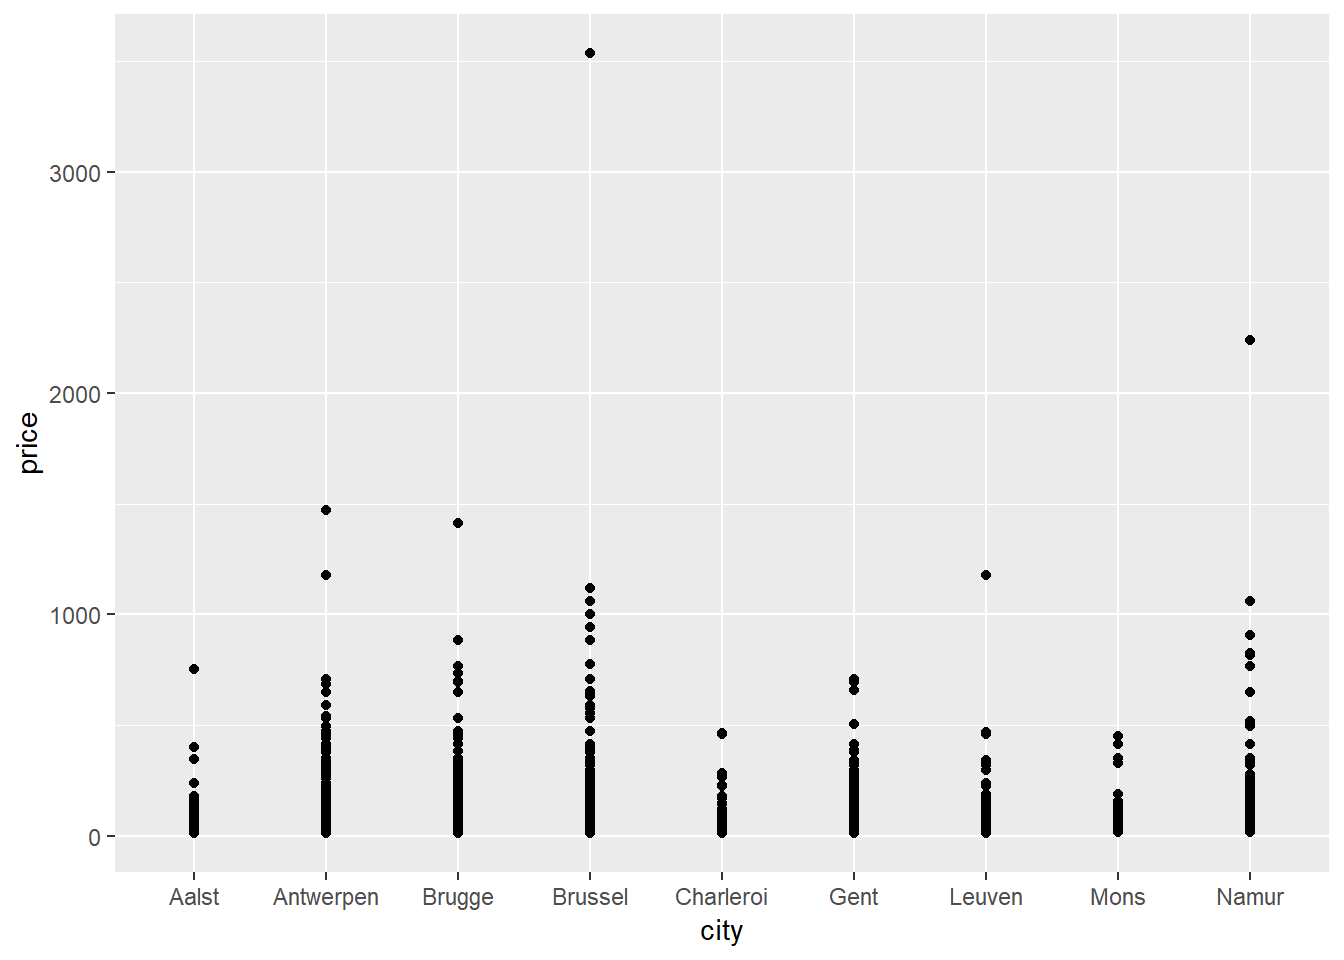
\includegraphics[width=12cm,height=8cm]{intro_scatterplot-1.png}
\end{center}

Se tudo correr bem, uma plotagem deve aparecer no canto inferior direito da tela. As figuras são feitas com o comando \fbox{ggplot}. Na primeira linha, você diz ao \fbox{ggplot} quais dados devem ser usados para criar um gráfico e quais variáveis devem aparecer no eixo X e no eixo Y. Dizemos para colocar cidade no eixo X e preço no eixo Y. A especificação do eixo X e do eixo Y sempre deve vir como argumentos para uma função aes, que por sua vez é fornecida como um argumento para a função \fbox{mapping} (mapeamento). Na segunda linha, você diz ao \fbox{ggplot} para desenhar pontos (\fbox{geom\_point}).

Ao criar um gráfico, lembre-se de sempre adicionar um \fbox{$+$} no final de cada linha de código que compõe o gráfico, exceto o último (adicionar o \fbox{$+$} no início de uma linha não funcionará).

O gráfico não é muito informativo porque muitos pontos são desenhados um sobre o outro.

\subsubsection{Jitter}

Vamos adicionar \fbox{jitter} aos nossos pontos:

\begin{lstlisting}[language=R]
ggplot(data = airbnb.topten, mapping = aes(x = city, y = price)) + 
  geom_jitter() # O mesmo codigo de antes mas agora mudamos geom_point para geom_jitter.
\end{lstlisting}

\begin{center}
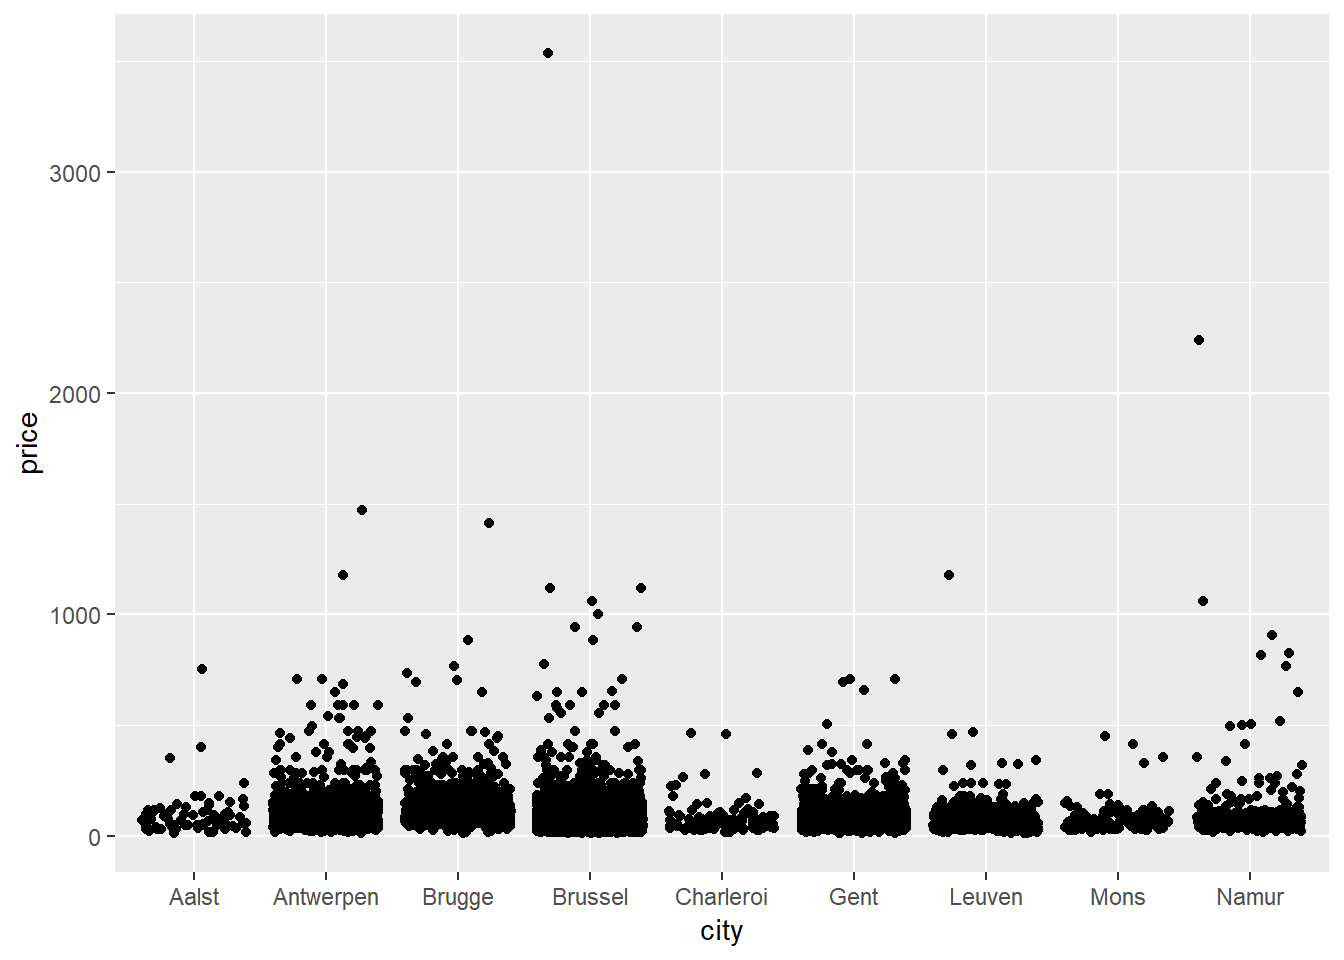
\includegraphics[width=12cm,height=8cm]{intro_jitter-1.png}
\end{center}

Em vez de solicitar pontos com \fbox{geom\_point()}, agora solicitamos pontos com \fbox{jitter} adicionado com \fbox{geom\_jitter()}. Jitter é um valor aleatório que é adicionado a cada coordenada X e Y, de modo que os pontos de dados não sejam desenhados um sobre o outro. Observe que fazemos isso apenas para tornar o gráfico mais informativo (compare-o com o gráfico de dispersão anterior, onde muitos pontos de dados são desenhados um sobre o outro); não altera os valores reais em nosso conjunto de dados.

\subsubsection{Histograma}

Ainda não está claro. Parece que a distribuição do preço está correta. Isso significa que a distribuição do preço não é normal. Uma distribuição normal tem dois recursos principais.

Uma primeira característica é que existem mais valores próximos à média do que valores distantes da média.

Em outras palavras, valores extremos não ocorrem com muita frequência.

Uma segunda característica é que a distribuição é simétrica. Em outras palavras, o número de valores abaixo da média é igual ao número de valores acima da média. Em uma distribuição distorcida, existem valores extremos em apenas um lado da distribuição. No caso de inclinação à direita, isso significa que existem valores extremos no lado direito da distribuição.

No nosso caso, isso significa que existem algumas listagens do Airbnb com preços muito altos. Isso aumenta a média da distribuição, de modo que as listagens não sejam mais normalmente distribuídas em torno da média.

Vamos desenhar um histograma dos preços:

\begin{lstlisting}[language=R]
ggplot(data = airbnb.topten, mapping = aes(x = price)) + # Observe que nao temos mais uma cidade x =. O preco deve estar no eixo X e as frequencias dos precos devem estar no eixo Y
  geom_histogram() # Eixo Y = frequencia dos valores no eixo X
\end{lstlisting}


\begin{center}
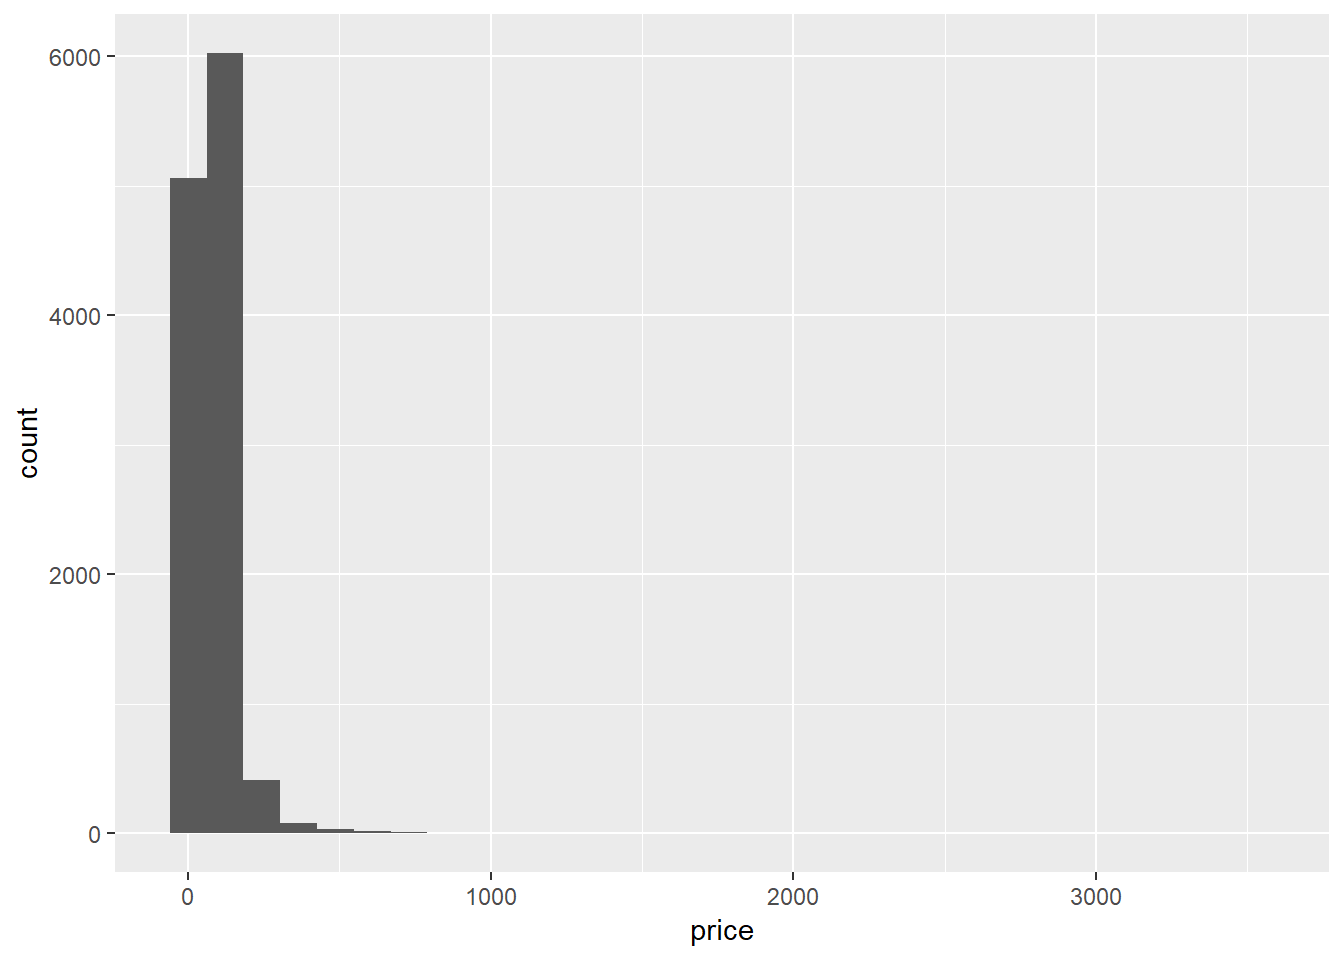
\includegraphics[width=12cm,height=8cm]{intro_histogram-1.png}
\end{center}

De fato, existem alguns preços extremamente altos (em comparação com a maioria dos preços), portanto, os preços estão inclinados à direita. Nota: o \fbox{stat\_bin()} usando compartimentos = 30. Escolha um valor melhor com o aviso de largura de caixa no console que possa ser ignorado com segurança.

\newpage
\subsubsection{Transformação logarítmica}

Como a variável \fbox{price} está inclinada à direita, podemos transformá-la em log para torná-la mais normal:

\begin{lstlisting}[language=R]
# No eixo y agora temos log(price, base=exp(1)) ao inves de price. log(price, base=exp(1)) = assuma o log natural, i.e., o log com base = exp(1) = e.

ggplot(data = airbnb.topten, mapping = aes(x = city, y = log(price, base=exp(1)))) + 
  geom_jitter()
\end{lstlisting}


\begin{center}
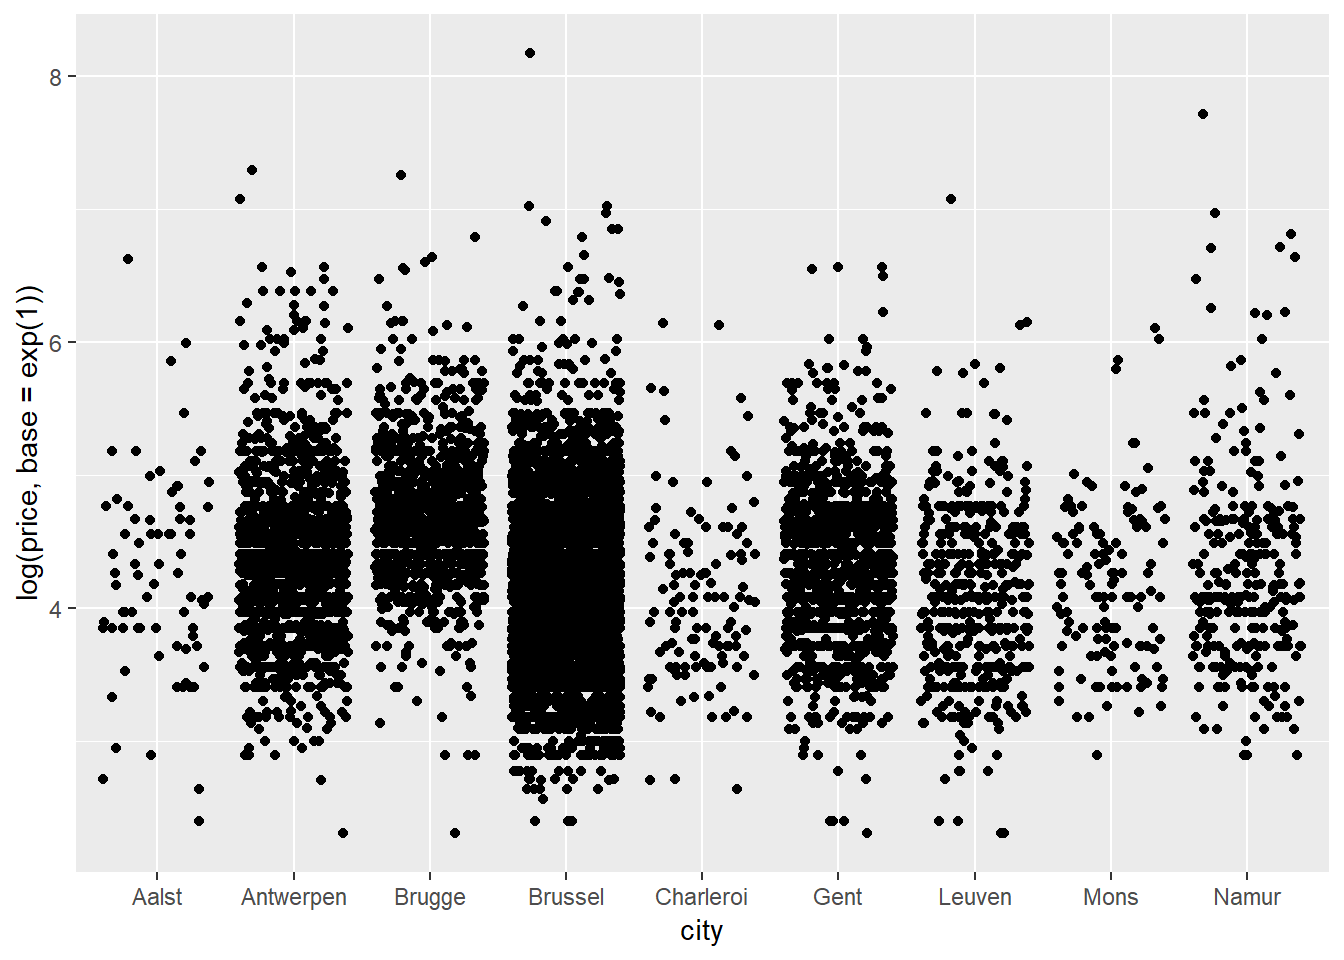
\includegraphics[width=12cm,height=8cm]{intro_log_transform-1.png}
\end{center}

\subsubsection{Plotando a mediana}

Vamos ter uma idéia melhor da mediana de preço por cidade:

\begin{lstlisting}[language=R]
ggplot(data = airbnb.topten, mapping = aes(x = city, y = price)) + 
  geom_jitter() +
  stat_summary(fun.y=median, colour="tomato3", size = 4, geom="point")
\end{lstlisting}

\begin{center}
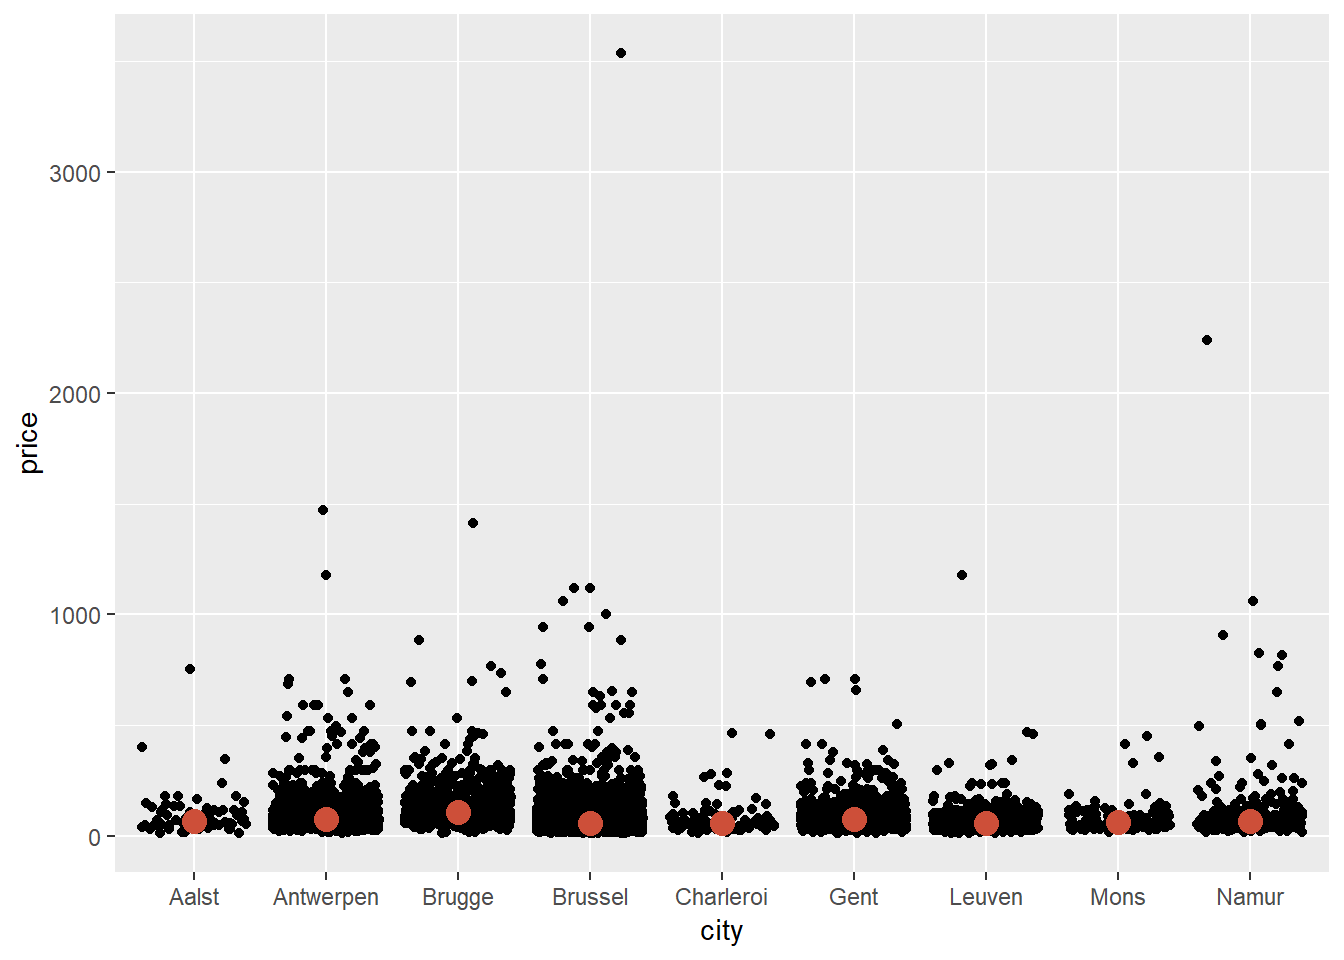
\includegraphics[width=12cm,height=8cm]{intro_median-1.png}
\end{center}

A linha de código para obter a mediana pode ser lida da seguinte forma: \fbox{stat\_summary} solicitará um resumo estatístico. A estatística que queremos é a mediana em uma cor chamada \fbox{"tomato3"}, com tamanho 4. Ela deve ser representada como um "ponto". Vemos que Bruges é a cidade com o preço mediano mais alto. É muito mais fácil ver isso quando transformamos o preço por log:

\begin{lstlisting}[language=R]
ggplot(data = airbnb.topten, mapping = aes(x = city, y = log(price, base = exp(1)))) + 
  geom_jitter() +
  stat_summary(fun.y=median, colour="tomato3", size = 4, geom="point")
\end{lstlisting}


\begin{center}
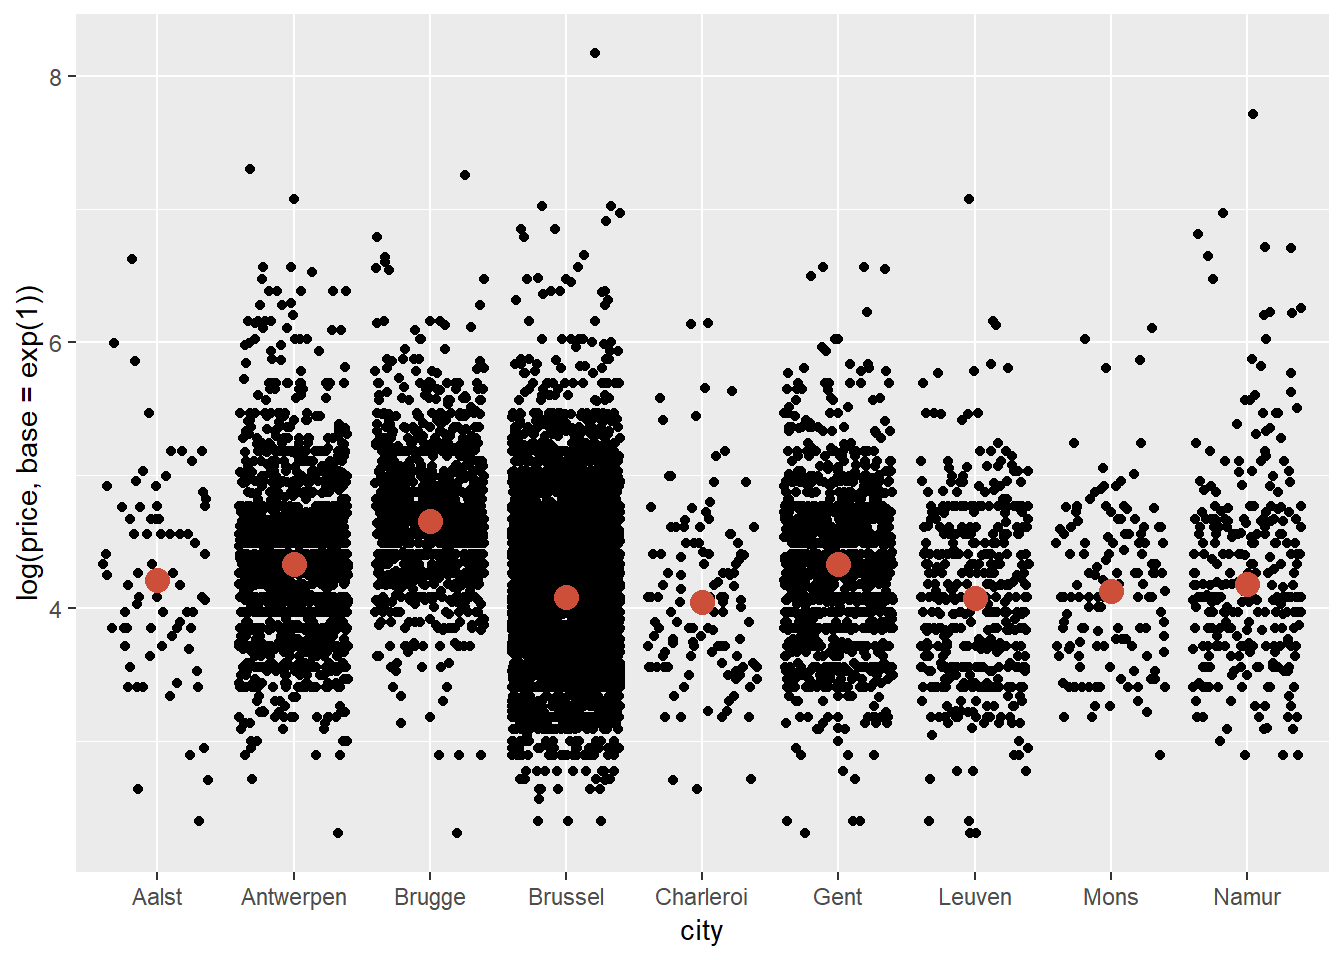
\includegraphics[width=12cm,height=8cm]{intro_plot_log_mean-1.png}
\end{center}

\subsubsection{Plota a média}

Vamos adicionar a média também, mas com uma cor e forma diferentes da média:

\begin{lstlisting}[language=R]
ggplot(data = airbnb.topten, mapping = aes(x = city, y = log(price, base = exp(1)))) + 
  geom_jitter() +
  stat_summary(fun.y=median, colour="tomato3", size = 4, geom="point") +
  stat_summary(fun.y=mean,   colour="green",   size = 4, geom="point", shape = 23, fill = "green")
\end{lstlisting}

\begin{center}
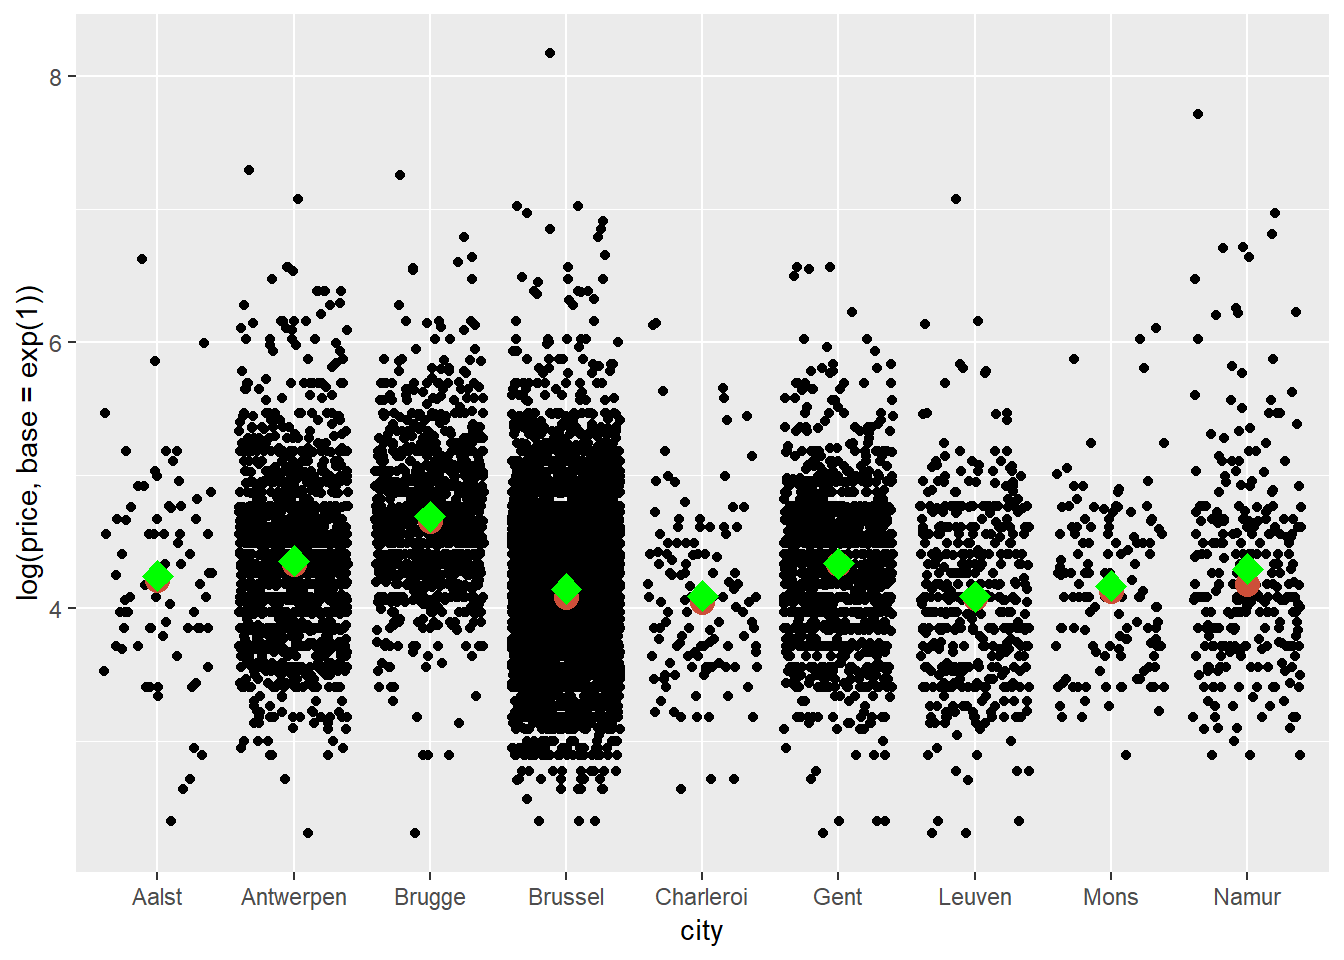
\includegraphics[width=12cm,height=8cm]{intro_plot_mean-1.png}
\end{center}

O código para obter a média é muito semelhante ao usado para obter a mediana. Simplesmente alteramos a estatística, a cor e adicionamos a forma = 23 para obter diamantes em vez de círculos e preencher = \fbox{"green"} para preencher os diamantes (pontos do gráfico). Vemos que os meios e medianas são bastante semelhantes.

\newpage
\subsubsection{Salvando imagens}

Podemos salvar esse gráfico em nosso disco rígido. Para fazer isso, clique em Exportar / Salvar como imagem. Se você não alterar o diretório, o arquivo será salvo no seu diretório de trabalho. Você pode redimensionar a plotagem e também fornecer um nome de arquivo significativo - Rplot01.png não será útil quando você tentar encontrar o arquivo posteriormente.

Uma maneira diferente (reproduzível) de salvar seu arquivo é agrupar o código nas funções \fbox{png()} e \fbox{dev.off()}:

\begin{lstlisting}[language=R]
png("price_per_city.png", width=800, height=600) 
# Isso ira preparar o R para salvar o grafico a seguir. 
# Fornece um nome de arquivo e dimensoes para largura e altura da figura em pixels

ggplot(data = airbnb.topten, mapping = aes(x = city, log(price, base = exp(1)))) + 
  geom_jitter() +
  stat_summary(fun.y=mean, colour="green", size = 4, geom="point", shape = 23, fill = "green") # Somente mantivemos a media aqui

dev.off() # Isso dira ao R que terminamos a plotagem e que ela deve salvar a plotagem no disco rigido.
\end{lstlisting}

Embora o \faRProject tenha uma interface não gráfica, ele pode criar gráficos muito bons. Praticamente todos os pequenos detalhes no gráfico podem ser ajustados. Muitos dos gráficos que você vê em "jornalismo de dados" (por exemplo, em \href{https://www.nytimes.com/}{https://www.nytimes.com/} ou em \href{http://fivethirtyeight.com/}{http://fivethirtyeight.com/}) são feitos em \faRProject.

\newpage
\section{Análise básica de dados: analisando dados secundários}

Neste capítulo, analisaremos os dados do Airbnb.com. A introdução tem mais informações sobre esses dados.

\subsection{Dados}
\subsubsection{Importação}

Você pode baixar o conjunto de dados clicando com o botão direito do mouse \href{http://users.telenet.be/samuelfranssens/tutorial_data/tomslee_airbnb_belgium_1454_2017-07-14.csv}{nesse link}, selecionando “Salvar link como…” (ou algo semelhante) e salvando o arquivo .csv em um diretório no disco rígido. Como mencionado na introdução, é uma boa ideia salvar seu trabalho em um diretório que é automaticamente copiado pelo software de compartilhamento de arquivos. Vamos importar os dados:


\begin{lstlisting}[language=R]
library(tidyverse)
setwd("c:/Dropbox/work/teaching/R/") # Ajusta seu diretorio de trabalho

airbnb <- read_csv("tomslee_airbnb_belgium_1454_2017-07-14.csv") %>% 
  mutate(room_id = factor(room_id), host_id = factor(host_id)) %>% 
  select(-country, -survey_id) %>% # dropa country & survey_id, veja a introdução de por que fazemos isso
  rename(country = city, city = borough) # renomeia city & borough, veja a introdução de por que fazemos isso
\end{lstlisting}

Não se esqueça de salvar seu script no diretório de trabalho.

\subsubsection{Manipulação}

Se você abrir o quadro de dados do airbnb em uma guia do Visualizador, verá que os \fbox{bathrooms} e o \fbox{minstay} são colunas vazias e que o \fbox{local} e \fbox{last\_modified} não são muito informativos. Vamos remover estas variáveis:

\begin{lstlisting}[language=R]
airbnb <- airbnb %>% 
  select (-bathrooms, -minstay, -location, -last_modified)
\end{lstlisting}

Agora, dê uma olhada na variável \fbox{overall\_satisfaction:}

\begin{lstlisting}
# use head() para imprimir apenas os primeiros valores de um vetor, para evitar uma lista muito longa
# tail() imprime apenas os últimos valores de um vetor
head (satisfação geral do airbnb $)

## [1] 4.5 0.0 4.0 4.5 5.0 5.0
\end{lstlisting}

A segunda classificação é zero. Provavelmente, isso significa que a classificação está faltando, em vez de ser realmente zero. Vamos substituir os valores zero na \fbox{overall\_satisfaction} por NA:

\begin{lstlisting}[language=R]
airbnb <- airbnb %>% 
  mutate(overall_satisfaction = replace(overall_satisfaction, overall_satisfaction == 0, NA)) 
  
# crie uma variavel "nova" overall_satisfaction que seja igual a overall_satisfaction com valores de NA em que overall_satisfaction seja igual a zero.

# Digamos que desejassemos substituir NA por 0, entao o comando se tornaria: substitute(overall_satisfaction, is.na(overall_satisfaction), 0)
# overall_satisfaction == NA nao funciona

head(airbnb$overall_satisfaction)

## [1] 4.5  NA 4.0 4.5 5.0 5.0
\end{lstlisting}

\newpage
\subsubsection{Mesclando datasets}

Posteriormente, testaremos se o preço está relacionado a determinadas características dos tipos de quartos. As características potencialmente interessantes são: \fbox{room\_type}, \fbox{city}, \fbox{reviews}, \fbox{overall\_satisfaction}, etc. Para torná-lo ainda mais interessante, podemos aumentar os dados, por exemplo, com dados disponíveis publicamente nas cidades. Reuni os tamanhos de população das cidades belgas mais populosas \href{https://population.mongabay.com/population/belgium/}{deste site}. Faça o download desses dados \href{http://users.telenet.be/samuelfranssens/tutorial_data/population.xlsx}{aqui} e importe-os para o \faRProject:

\begin{lstlisting}[language=R]
population <- read_excel("population.xlsx","data")
population

## # A tibble: 183 x 2
##    place     population
##    <chr>          <dbl>
##  1 Brussels     1019022
##  2 Antwerpen     459805
##  3 Gent          231493
##  4 Charleroi     200132
##  5 Liège         182597
##  6 Brugge        116709
##  7 Namur         106284
##  8 Leuven         92892
##  9 Mons           91277
## 10 Aalst          77534
## # ... with 173 more rows
\end{lstlisting}


Agora, queremos vincular esses dados ao nosso quadro de dados do airbnb. Isso é muito fácil no \faRProject (mas é muito difícil, por exemplo, no Excel):

\begin{lstlisting}[language=R]
airbnb.merged <- left_join(airbnb, population, by = c("city" = "place"))
# o primeiro argumento eh o conjunto de dados que queremos aumentar
# o segundo argumento eh onde encontramos os dados para aumentar o primeiro conjunto de dados com
# o terceiro argumento sao as variaveis que usamos para vincular um conjunto de dados ao outro (cidade eh uma variavel no airbnb, local eh uma variavel na populacao)   
\end{lstlisting}

Confira as colunas mais relevantes do quadro de dados airbnb.merged:

\begin{lstlisting}[language=R]
airbnb.merged %>% select(room_id, city, price, population)

## # A tibble: 17,651 x 4
##    room_id  city     price population
##    <fct>    <chr>    <dbl>      <dbl>
##  1 5141135  Gent        59     231493
##  2 13128333 Brussel     53         NA
##  3 8298885  Brussel     46         NA
##  4 13822088 Oostende    56         NA
##  5 18324301 Brussel     47         NA
##  6 12664969 Brussel     60         NA
##  7 15452889 Gent        41     231493
##  8 3911778  Brussel     36         NA
##  9 14929414 Verviers    18      52824
## 10 8497852  Brussel     38         NA
## # ... with 17,641 more rows
\end{lstlisting}

Vemos que há uma \fbox{population} de colunas em nosso conjunto de dados \fbox{airbnb.merged}. Você também pode ver isso no painel Ambiente: \fbox{airbnb.merged} tem uma variável a mais que \fbox{airbnb} (mas o mesmo número de observações).

Faltam dados para Bruxelas, no entanto. Isso ocorre porque Bruxelas está escrito em holandês no conjunto de dados airbnb, mas em inglês no conjunto de dados da \fbox{population}. 
\newpage
Vamos substituir Bruxelas por Bruxelas no conjunto de dados da \fbox{population} (e também alterar a ortografia de duas outras cidades) e vincular os dados novamente:

\begin{lstlisting}[language=R]
population <- population %>% 
  mutate(place = replace(place, place == "Brussels", "Brussel"),
         place = replace(place, place == "Ostend", "Oostende"),
         place = replace(place, place == "Mouscron", "Moeskroen"))

airbnb.merged <- left_join(airbnb, population, by = c("city" = "place"))

airbnb.merged %>% select(room_id, city, price, population)

## # A tibble: 17,651 x 4
##    room_id  city     price population
##    <fct>    <chr>    <dbl>      <dbl>
##  1 5141135  Gent        59     231493
##  2 13128333 Brussel     53    1019022
##  3 8298885  Brussel     46    1019022
##  4 13822088 Oostende    56      69011
##  5 18324301 Brussel     47    1019022
##  6 12664969 Brussel     60    1019022
##  7 15452889 Gent        41     231493
##  8 3911778  Brussel     36    1019022
##  9 14929414 Verviers    18      52824
## 10 8497852  Brussel     38    1019022
## # ... with 17,641 more rows
\end{lstlisting}

\subsubsection{Recapitulando: importação e manipulação}

Aqui está o que fizemos até agora, em uma sequência ordenada de operações pipe (faça o download dos dados \href{http://users.telenet.be/samuelfranssens/tutorial_data/tomslee_airbnb_belgium_1454_2017-07-14.csv}{aqui} e \href{http://users.telenet.be/samuelfranssens/tutorial_data/population.xlsx}{aqui}):

\begin{lstlisting}[language=R]
library(tidyverse)
setwd("c:/Dropbox/work/teaching/R") # Configura seu diretorio de trabalho

airbnb <- read_csv("tomslee_airbnb_belgium_1454_2017-07-14.csv") %>% 
  mutate(room_id = factor(room_id), host_id = factor(host_id),
         overall_satisfaction = replace(overall_satisfaction, overall_satisfaction == 0, NA)) %>% 
  select(-country, -survey_id,- bathrooms, -minstay, -location, -last_modified) %>% 
  rename(country = city, city = borough) 

population <- read_excel("population.xlsx","data") %>% 
  mutate(place = replace(place, place == "Brussels", "Brussel"),
         place = replace(place, place == "Ostend", "Oostende"),
         place = replace(place, place == "Mouscron", "Moeskroen"))

airbnb <- left_join(airbnb, population, by = c("city" = "place"))
\end{lstlisting}


\subsection{Amostras independentes: teste t}

Digamos que queremos testar se os preços diferem entre cidades grandes e pequenas. Para fazer isso, precisamos de uma variável que indique se um Airbnb está em uma cidade grande ou pequena. Na Bélgica, consideramos cidades com uma população de pelo menos cem mil como grande:

\begin{lstlisting}[language=R]
airbnb <- airbnb %>% 
  mutate(large = population > 100000,
         size = factor(large, labels = c("small","large")))

# Nos poderiamos tambem ter escrito: mutate(size = factor(population > 100000, labels = c("small","large)))

# observando a variavel populacao
head(airbnb$population)

## [1]  231493 1019022 1019022   69011 1019022 1019022

# olhando a maior variavel
head(airbnb$large)

## [1]  TRUE  TRUE  TRUE FALSE  TRUE  TRUE

# e o tamanho da variavel
head(airbnb$size)

## [1] large large large small large large
## Levels: small large
\end{lstlisting}

No script acima, primeiro criamos uma variável lógica (esse é outro tipo de variável; discutimos outras aqui). Chamamos essa variável de grande e é \fbox{TRUE} quando a população é maior que 100000 e \fbox{FALSE}, se não. Depois, criamos um novo tamanho de variável que é a fatoração de grande porte. Observe que adicionamos outro argumento à função \fbox{factor}, ou seja, \fbox{labels}, para fornecer os valores \fbox{large} de nomes mais intuitivos. \fbox{FALSE} vem em primeiro lugar no alfabeto e obtém o primeiro rótulo pequeno, \fbox{TRUE} fica em segundo lugar no alfabeto e obtém o segundo rótulo grande.

Para saber quais cidades são grandes e quais são pequenas, podemos solicitar frequências de combinações de tamanho (grande versus pequeno) e \fbox{city} (a própria cidade). Aprendemos como fazer isso no capítulo introdutório (consulte as tabelas de frequência e as estatísticas descritivas):

\begin{lstlisting}[language=R]
airbnb %>% 
  group_by(size, city) %>% 
  summarize(count = n(), population = mean(population)) %>% # Cidades formam os grupos. Portanto, a populacao media de um grupo = a media de observacoes com a mesma populacao, porque elas vem da mesma cidade = a populacao da cidade
  arrange(desc(size), desc(population)) %>% # maior cidade no topo
  print (n = Inf) # mostra a distribuicao completa das frequencias
  
  ## # A tibble: 43 x 4
## # Groups:   size [3]
##    size  city              count population
##    <fct> <chr>             <int>      <dbl>
##  1 large Brussel            6715    1019022
##  2 large Antwerpen          1610     459805
##  3 large Gent               1206     231493
##  4 large Charleroi           118     200132
##  5 large Liège               667     182597
##  6 large Brugge             1094     116709
##  7 large Namur               286     106284
##  8 small Leuven              434      92892
##  9 small Mons                129      91277
## 10 small Aalst                74      77534
## 11 small Mechelen            190      77530
## 12 small Kortrijk            107      73879
## 13 small Hasselt             151      69222
## 14 small Oostende            527      69011
## 15 small Sint-Niklaas         52      69010
## 16 small Tournai              97      67721
## 17 small Roeselare            41      56016
## 18 small Verviers            631      52824
## 19 small Moeskroen            28      52069
## 20 small Dendermonde          45      43055
## 21 small Turnhout            130      39654
## 22 small Ieper               143      35089
## 23 small Tongeren            173      29816
## 24 small Oudenaarde          110      27935
## 25 small Ath                  47      26681
## 26 small Arlon                46      26179
## 27 small Soignies             58      24869
## 28 small Nivelles            505      24149
## 29 small Maaseik              93      23684
## 30 small Huy                  99      19973
## 31 small Tielt                24      19299
## 32 small Eeklo                43      19116
## 33 small Marche-en-Famenne   266      16856
## 34 small Diksmuide            27      15515
## 35 <NA>  Bastogne            145         NA
## 36 <NA>  Dinant              286         NA
## 37 <NA>  Halle-Vilvoorde     471         NA
## 38 <NA>  Neufchâteau         160         NA
## 39 <NA>  Philippeville        85         NA
## 40 <NA>  Thuin                81         NA
## 41 <NA>  Veurne              350         NA
## 42 <NA>  Virton               56         NA
## 43 <NA>  Waremme              51         NA
\end{lstlisting}

Vemos que algumas cidades têm um valor de NA para tamanho. Isso ocorre porque não temos população para essas cidades (e, portanto, também não sabemos se é uma cidade grande ou pequena). Vamos filtrar essas observações e verificar as médias e os desvios padrão de preço, dependendo do tamanho da cidade:

\begin{lstlisting}[language=R]
airbnb.cities <- airbnb %>% 
  filter(!is.na(population)) 
# Filtre as observacoes para as quais nao temos a populacao.
# O ponto de exclamacao deve ser lido como NAO. Entao, queremos manter as observacoes para as quais a populacao NAO eh NA.
# Visite https://r4ds.had.co.nz/transform.html#filter-rows-with-filter para conhecer mais sobre operadores logicos (veja secao 5.2.2).

airbnb.cities %>% 
  group_by(size) %>% 
  summarize(mean_price = mean(price),
            sd_price = sd(price),
            count = n())

## # A tibble: 2 x 4
##   size  mean_price sd_price count
##   <fct>      <dbl>    <dbl> <int>
## 1 small      110.     122.   4270
## 2 large       85.4     82.5 11696
\end{lstlisting}

Vemos que os preços são mais altos nas pequenas e nas grandes cidades, mas queremos saber se essa diferença é significativa. Um teste t de amostras independentes pode fornecer a resposta (as listagens nas grandes cidades e as listagens nas pequenas cidades são as amostras independentes), mas precisamos verificar primeiro uma suposição: as variâncias das duas amostras independentes são iguais?

\begin{lstlisting}[language=R]
install.packages("car") # Para o teste de igualdade de variancias precisaremos do pacote car.
library(car)

# Teste de Levene para variancias iguais 
# Baixo valor p significa que as variancias nao sao iguais. 
# Primeiro argumento = variavel dependente continua, segundo argumento = variavel independente categorica.

leveneTest(airbnb.cities$price, airbnb.cities$size) 

## Levene's Test for Homogeneity of Variance (center = median)
##          Df F value    Pr(>F)    
## group     1  139.76 < 2.2e-16 ***
##       15964                      
## ---
## Signif. codes:  0 '***' 0.001 '**' 0.01 '*' 0.05 '.' 0.1 ' ' 1
\end{lstlisting}



A hipótese nula de variâncias iguais é rejeitada ($p <0,001$), portanto, devemos continuar com um teste $t$ que pressupõe variâncias desiguais:

\begin{lstlisting}[language=R]
# Teste se os preços médios das cidades grandes e pequenas são diferentes.
# Indique se o teste deve assumir variações iguais ou não (defina var.equal = TRUE para um teste que assume variações iguais).

t.test(airbnb.cities$price ~ airbnb.cities$size, var.equal = FALSE)

## 
##  Welch Two Sample t-test
## 
## data:  airbnb.cities$price by airbnb.cities$size
## t = 12.376, df = 5762.8, p-value < 2.2e-16
## alternative hypothesis: true difference in means is not equal to 0
## 95 percent confidence interval:
##  20.95129 28.83782
## sample estimates:
## mean in group small mean in group large 
##           110.31265            85.41809
\end{lstlisting}


Você pode relatar o seguinte: “As cidades grandes (M = 85,42, DP = 82,46) tinham um preço mais baixo (t (5762,79) = 12,376, p <0,001, variação desigual assumida) do que as cidades pequenas (M = 110,31, DP = 121,63). ”


\subsubsection{ANOVA univariada}

Quando sua variável independente (categórica) possui apenas dois grupos, é possível testar se as médias da variável dependente (contínua) são significativamente diferentes ou não com um teste $t$. Quando sua variável independente possui mais de dois grupos, você pode testar se as médias são diferentes com uma ANOVA.

Por exemplo, digamos que queremos testar se há uma diferença significativa entre os preços médios de casas e apartamentos inteiros, salas privadas e quartos compartilhados. Vamos dar uma olhada nos meios por tipo de quarto:

\begin{lstlisting}[language=R]
airbnb.summary <- airbnb %>% 
  group_by(room_type) %>% 
  summarize(count = n(), # obtenha as frequencias dos diferentes tipos de quartos 
            mean_price = mean(price), # o preco medio por tipo de quarto
            sd_price = sd(price)) # e o desvio padrao do preco por tipo de quarto

airbnb.summary

## # A tibble: 3 x 4
##   room_type       count mean_price sd_price
##   <chr>           <int>      <dbl>    <dbl>
## 1 Entire home/apt 11082      113.     118. 
## 2 Private room     6416       64.3     46.5
## 3 Shared room       153       49.6     33.9
\end{lstlisting}

Também podemos traçar esses meios em um gráfico de barras:

\begin{lstlisting}[language=R]
# Ao criar um grafico de barras, o conjunto de dados que serve como entrada para o ggplot eh o resumo com os meios, nao o conjunto de dados completo.
# (Eh por isso que salvamos o resumo acima em um objeto airbnb.summary)

ggplot(data = airbnb.summary, mapping = aes(x = room_type, y = mean_price)) + 
  geom_bar(stat = "identity", position = "dodge")
\end{lstlisting}

\begin{center}
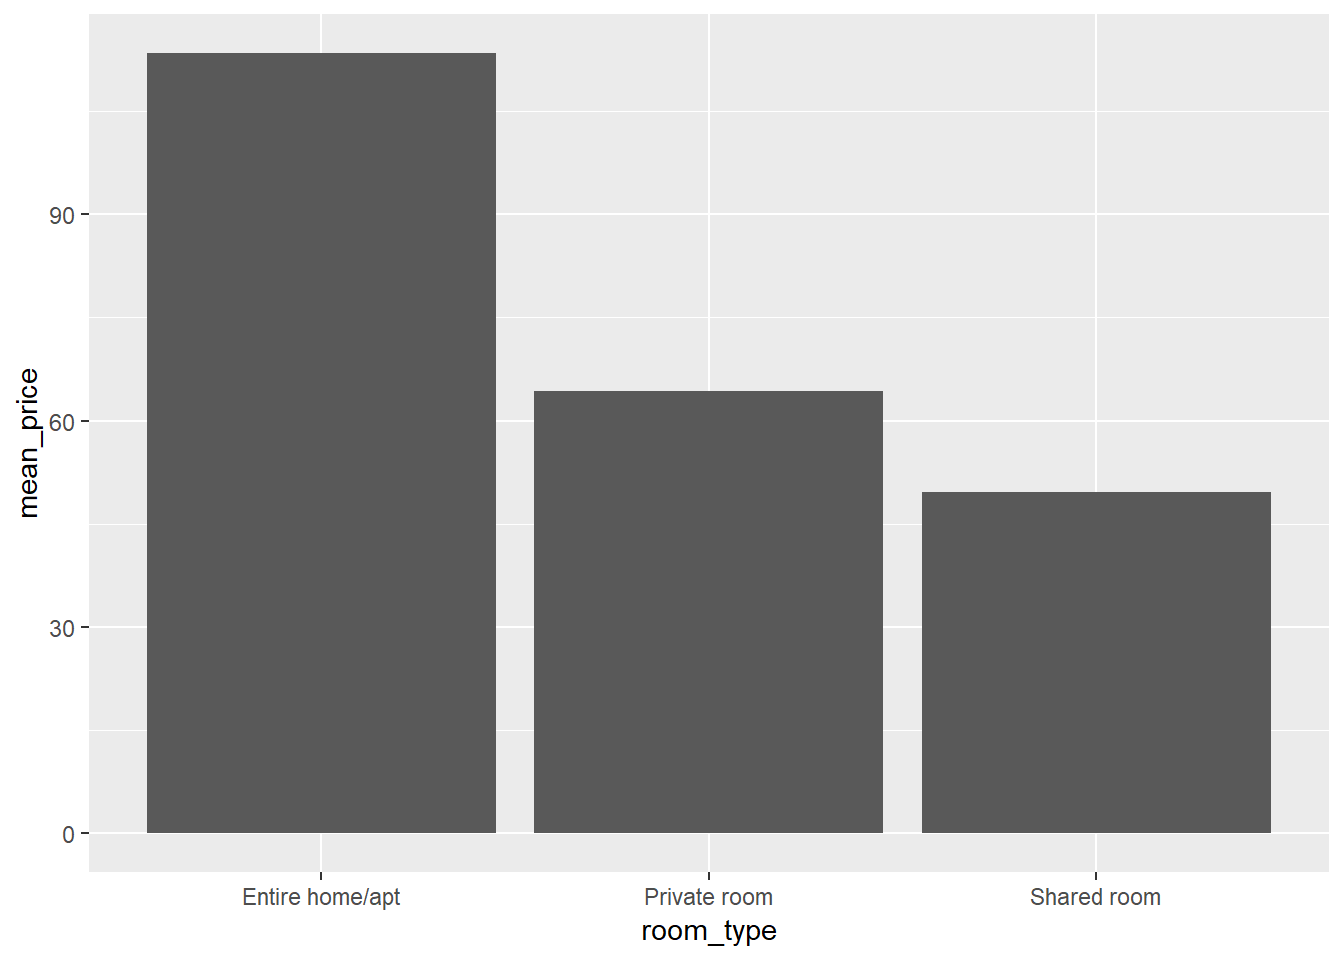
\includegraphics[width=12cm,height=8cm]{modelling_oneway_barplot-1.png} 
\end{center}

Não é de surpreender que casas ou apartamentos inteiros tenham preços mais altos do que quartos particulares, que, por sua vez, têm preços mais altos que quartos compartilhados. Também vemos que há quase o dobro de casas e apartamentos inteiros do que quartos privativos disponíveis e quase não há quartos compartilhados disponíveis. Além disso, o desvio padrão é muito mais alto na categoria de casas ou apartamentos inteiros do que nas categorias de quarto particular ou compartilhado.

Uma ANOVA pode testar se há diferenças significativas nos preços médios por tipo de quarto. Porém, antes de executar uma ANOVA, precisamos verificar se as premissas da ANOVA são atendidas.

\newpage

\subsubsection{Suposição: normalidade de resíduos}

A primeira suposição é que a variável dependente (\fbox{price}) é normalmente distribuída em cada nível da variável independente (\fbox{room\_type}). Primeiro, vamos inspecionar visualmente se essa suposição será válida:

\begin{lstlisting}[language=R]

# Ao criar um histograma, o conjunto de dados que serve como entrada para o ggplot eh o conjunto de dados completo, nao o resumo com os meios

ggplot(data = airbnb, mapping = aes(x = price)) + # Queremos price no eixo x.
  facet_wrap(~ room_type) + # Queremos que isso seja dividido por room_type.
  #facet_wrap garantira que o ggplot crie paineis diferentes no seu gráfico.
  geom_histogram() # geom_histogram garante que as frequencias dos valores no eixo X sejam plotadas.
  ## `stat_bin()` using `bins = 30`. Pega o melhor valor com `binwidth`.
\end{lstlisting}


\begin{center}
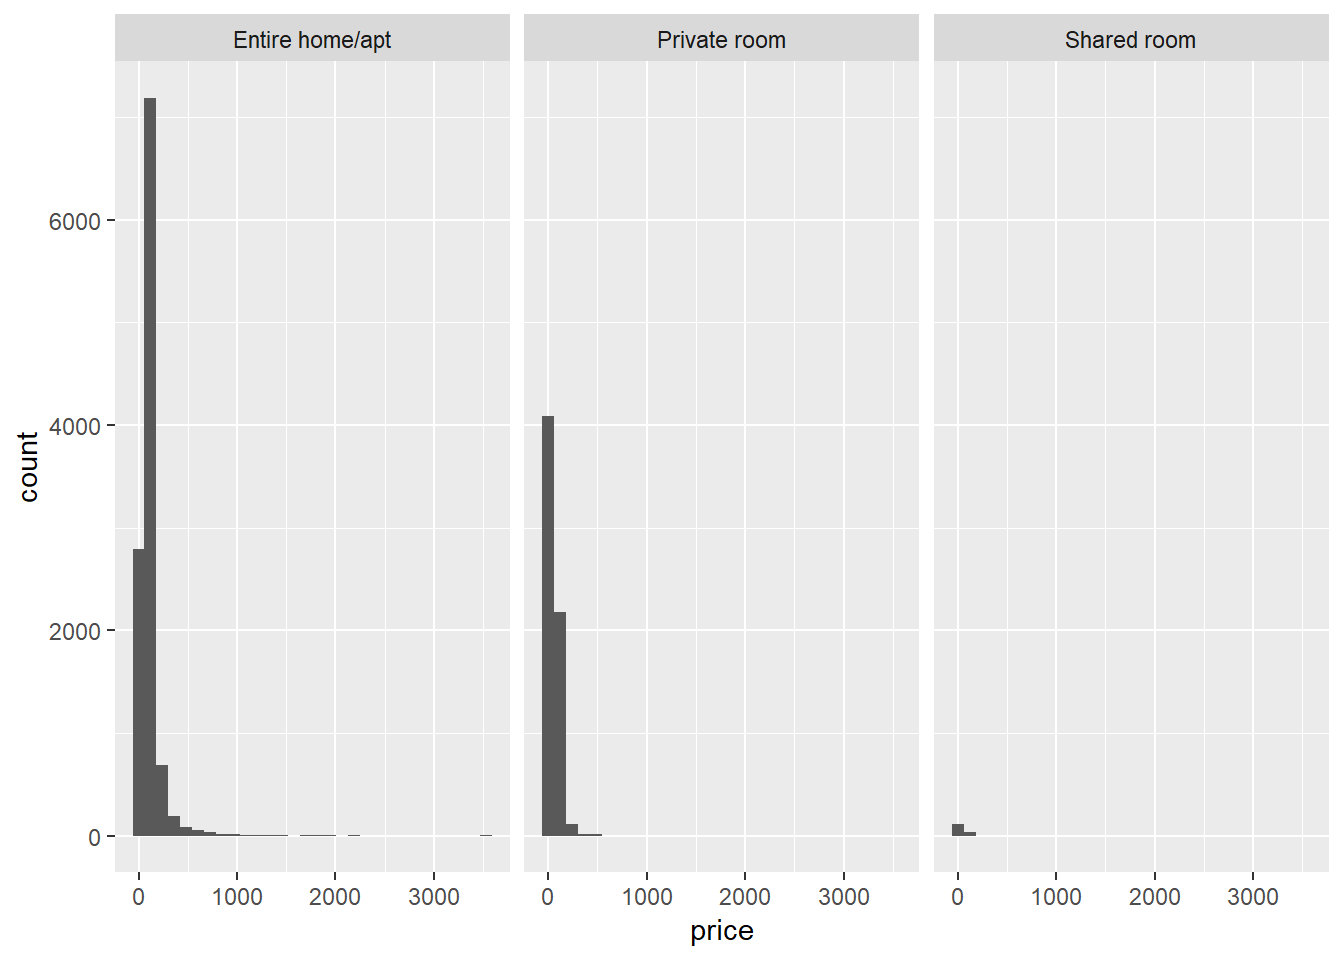
\includegraphics[width=12cm,height=8cm]{modelling_histogram-1.png} 
\end{center}

Vemos que há inclinação correta para cada tipo de sala. Também podemos testar formalmente, dentro de cada tipo de sala, se as distribuições são normais com o teste Shapiro-Wilk. Por exemplo, para as salas compartilhados:

\begin{lstlisting}[language=R]
airbnb.shared <- airbnb %>% 
  filter(room_type == "Shared room") # reter dados apenas das salas compartilhadas

shapiro.test(airbnb.shared$price)

## 
##  Shapiro-Wilk normality test
## 
## data:  airbnb.shared$price
## W = 0.83948, p-value = 1.181e-11

\end{lstlisting}

O valor-p deste teste é extremamente pequeno, portanto a hipótese nula de que a amostra provém de uma distribuição normal deve ser rejeitada. Se tentarmos o teste Shapiro-Wilk para as salas privadas:

\begin{lstlisting}[language=R]

airbnb.private <- airbnb %>% 
  filter(room_type == "Private room") # armazenar dados apenas das salas compartilhadas
  
shapiro.test(airbnb.private$price)

## Error in shapiro.test(airbnb.private$price): sample size must be between 3 and 5000
\end{lstlisting}

Ocorreu um erro ao dizer que o tamanho da amostra é muito grande. Para contornar esse problema, podemos tentar o teste Anderson-Darling do pacote \fbox{nortest}:

\newpage
\begin{lstlisting}[language=R]
install.packages("nortest")
library(nortest)
ad.test(airbnb.private$price)

## 
##  Anderson-Darling normality test
## 
## data:  airbnb.private$price
## A = 372.05, p-value < 2.2e-16
\end{lstlisting}

Mais uma vez, rejeitamos a hipótese nula de normalidade. Deixo como exercício para testar a normalidade dos preços de casas e apartamentos inteiros.

Agora que sabemos que a suposição de normalidade é violada, o que podemos fazer? Podemos considerar transformar nossa variável dependente com uma transformação de log:

\begin{lstlisting}[language=R]
ggplot(data=airbnb, mapping=aes(x=log(price, base = exp (1)))) + # Queremos o preco transformado em log no eixo X.
   facet_wrap(~ room_type) + # Queremos que isso seja dividido por room_type. Facet_wrap garantira que o ggplot crie paineis diferentes no seu grafico.
   geom_histogram() # geom_histogram garante que as frequencias dos valores no eixo X sejam plotadas.
   
   ## `stat_bin()` using `bins = 30`. Pega um valor melhor com `binwidth`.
\end{lstlisting}

\begin{center}
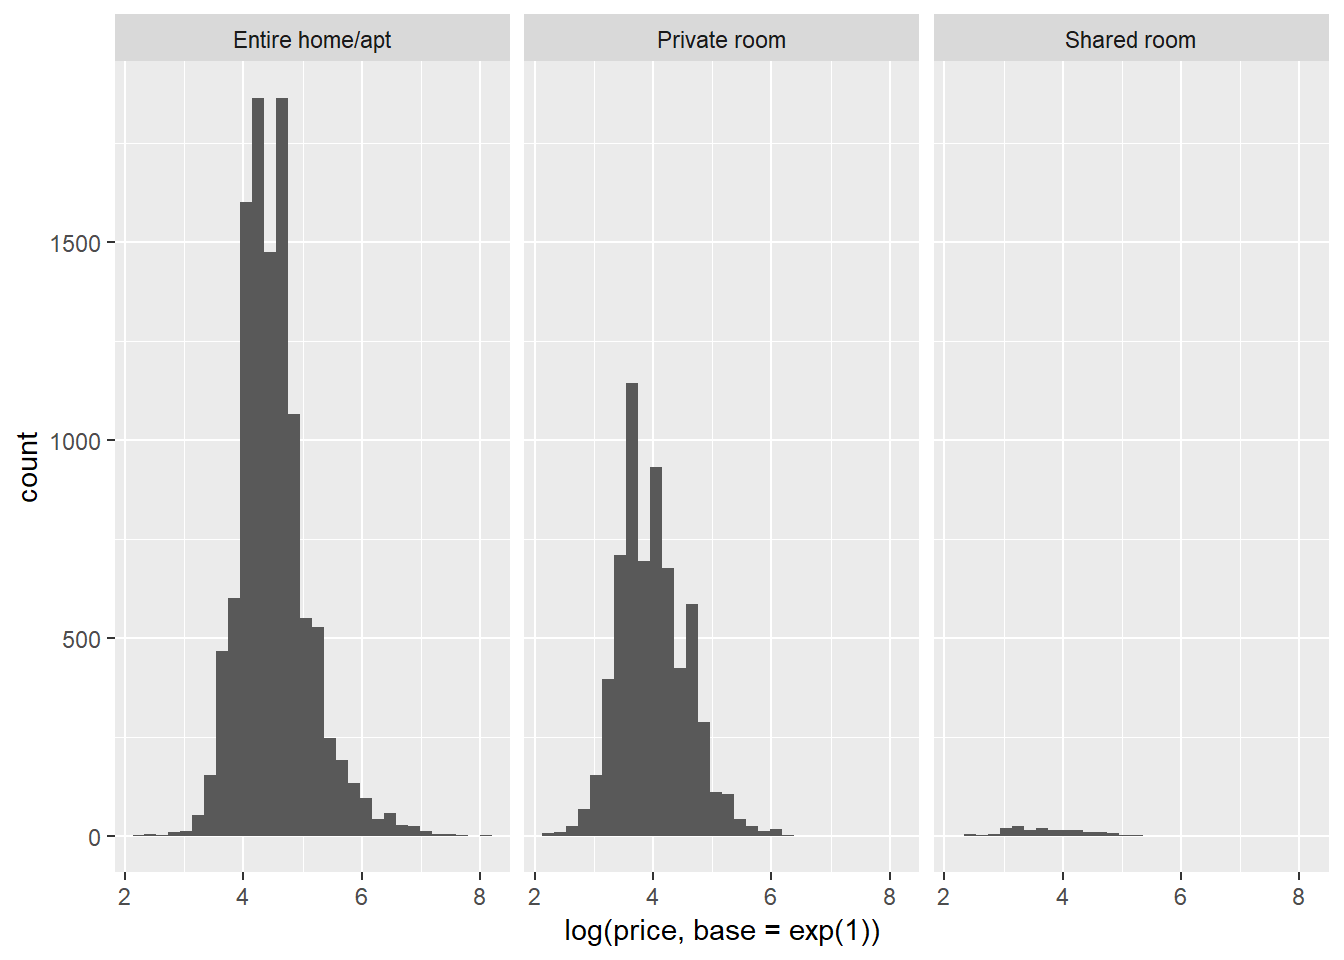
\includegraphics[width=12cm,height=8cm]{modelling_logtransform-1.png} 
\end{center}

Como você pode ver, uma transformação de log normaliza uma distribuição inclinada à direita. Poderíamos então executar a ANOVA na variável dependente transformada em log. No entanto, na realidade, muitas vezes é seguro ignorar violações da suposição de normalidade (a menos que você esteja lidando com pequenas amostras, o que nós não somos). Vamos simplesmente continuar com o preço não transformado como variável dependente.


\subsubsection{Suposição: homogeneidade de variâncias}

Uma segunda suposição que precisamos verificar é se as variações de nosso preço variável dependente são iguais nas categorias de nossa variável independente \fbox{room\_type}. Normalmente, um gráfico boxplot é informativo:

\begin{lstlisting}[language=R]
ggplot(data = airbnb, mapping = aes(x = room_type, y = price)) + 
  geom_boxplot()
\end{lstlisting}

\begin{center}
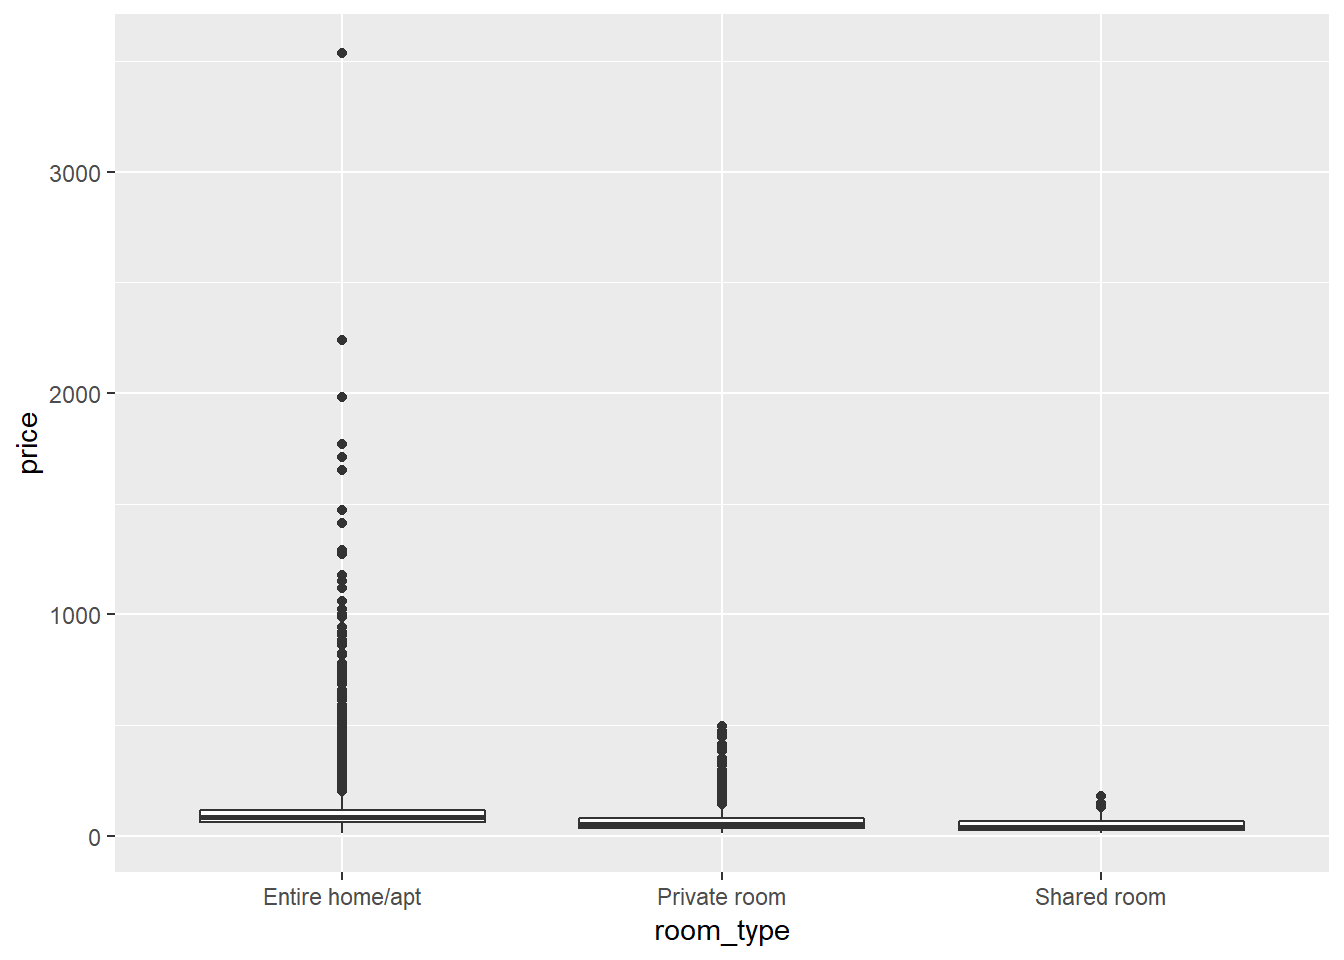
\includegraphics[width=12cm,height=8cm]{modelling_boxplot2-1.png} 
\end{center}

Mas, neste caso, os intervalos interquartis (as alturas das caixas), que normalmente nos dariam uma idéia da variação dentro de cada tipo de quarto, são muito estreitos. Isso ocorre porque o intervalo de valores Y a ser plotado é muito amplo devido a alguns valores extremos. Se observarmos os desvios padrão, porém, veremos que estes são muito maiores para todos as salas e apartamentos do que para os quartos privativo e compartilhado:

\begin{lstlisting}[language=R]
airbnb %>% 
  group_by(room_type) %>% 
  summarize(count = n(), # obtenha as frequencias dos diferentes tipos de quartos
            mean_price = mean(price), # o preco medio por tipo de quarto
            sd_price = sd(price)) # e o desvio padrao do preco por tipo de quarto
            
## # A tibble: 3 x 4
##   room_type       count mean_price sd_price
##   <chr>           <int>      <dbl>    <dbl>
## 1 Entire home/apt 11082      113.     118. 
## 2 Private room     6416       64.3     46.5
## 3 Shared room       153       49.6     33.9
\end{lstlisting}

Também podemos realizar um teste formal de homogeneidade de variâncias. Para isso, precisamos da função \fbox{leveneTest} do pacote \fbox{car}:

\begin{lstlisting}[language=R]
install.packages("car") # Para o teste de variancias iguais, precisamos de um pacote chamado car. Instalamos isso antes, portanto, nao eh necessario reinstala-lo se voce ja o tiver feito.

library(car)

#Teste de Levene de variancias iguais.
# Valor baixo de p significa que as variancias nao sao iguais.
# Primeiro argumento = variavel dependente continua, segundo argumento = variavel independente categorica.

leveneTest(airbnb$price, airbnb$room_type) 

## Levene's Test for Homogeneity of Variance (center = median)
##          Df F value    Pr(>F)    
## group     2  140.07 < 2.2e-16 ***
##       17648                      
## ---
## Signif. codes:  0 '***' 0.001 '**' 0.01 '*' 0.05 '.' 0.1 ' ' 1
\end{lstlisting}

Como o valor p é extremamente pequeno, rejeitamos a hipótese nula de variâncias iguais. Assim como no pressuposto da normalidade, as violações do pressuposto de variâncias iguais podem, no entanto, ser frequentemente ignoradas e o faremos neste caso.

\newpage

\subsection{ANOVA}

Para realizar uma ANOVA, precisamos instalar alguns pacotes:

\begin{lstlisting}[language=R]
install.packages("remotes") #O pacote de controles remotos nos permite instalar pacotes armazenados no GitHub, um site para desenvolvedores de pacotes. 
install.packages("car") #Também precisaremos do pacote do carro para executar a ANOVA (não é necessário reinstalá-lo se você já tiver feito isso).

library(remotes)
install_github('samuelfranssens/type3anova') # Instala o pacote type3anova. Esta e as etapas anteriores precisam ser executadas apenas uma vez.

library(type3anova) # Carregue o pacote type3anova.
\end{lstlisting}

Agora podemos prosseguir com a ANOVA verdadeira:

\begin{lstlisting}[language=R]
# Primeiro cria um modelo linear
# A formula lm() toma os argumentos de dados 
# A fórmula tem a seguinte sintaxe: variável dependente ~ variável (s) independente

linearmodel <- lm(price ~ room_type, data=airbnb) 

# Em seguida, peça a saída no formato ANOVA. Isso fornece a soma dos quadrados do Tipo III. 
# Observe que isso é diferente da anova (modelo linear), que fornece a soma dos quadrados do tipo I.

type3anova(linearmodel) 

## # A tibble: 3 x 6
##   term                ss   df1   df2     f     pvalue
##   <chr>            <dbl> <dbl> <int> <dbl>      <dbl>
## 1 (Intercept)   7618725.     1 17648  803.  7.31e-173
## 2 room_type    10120155.     2 17648  534.  1.02e-225
## 3 Residuals   167364763. 17648 17648   NA  NA
\end{lstlisting}

Nesse caso, o valor-p associado ao efeito de \fbox{room\_type} é praticamente 0, o que significa que rejeitamos a hipótese nula de que o preço médio é igual para cada \fbox{room\_type}. Você pode relatar o seguinte: “Houve diferenças significativas entre os preços médios das diferentes tipos de salas ($F (2, 17648) = 533,57, p <0,001$).”

\subsection{Teste de Tuckey de diferença significativa verdadeira}

Observe que a ANOVA testa a hipótese nula de que as médias em todos os nossos grupos são iguais. A rejeição desta hipótese nula significa que há uma diferença significativa em pelo menos um dos possíveis pares de médias (ou seja, em casa / apartamento inteiro vs. privado e / ou em casa / apartamento inteiro vs. compartilhado e / ou privado) vs. compartilhado). Para ter uma idéia de qual par de médias contém uma diferença significativa, podemos acompanhar o teste de Tukey, que nos dará todas as comparações pareadas.


O teste de Tukey corrige os valores de p para cima - portanto, é mais conservador decidir que algo é significativo - porque as comparações são post-hoc ou exploratórias:

\begin{lstlisting}[language=R]
TukeyHSD(aov(price ~ room_type, data=airbnb), 
         "room_type") # O primeiro argumento eh um objeto "aov", o segundo eh a nossa variavel independente.
         
##   Tukey multiple comparisons of means
##     95% family-wise confidence level
## 
## Fit: aov(formula = price ~ room_type, data = airbnb)
## 
## $room_type
##                                   diff       lwr        upr    p adj
## Private room-Entire home/apt -49.11516 -52.69593 -45.534395 0.000000
## Shared room-Entire home/apt  -63.79178 -82.37217 -45.211381 0.000000
## Shared room-Private room     -14.67661 -33.34879   3.995562 0.155939
\end{lstlisting}

Isso nos mostra que não há diferença significativa no preço médio de quartos compartilhados e privados, mas que quartos compartilhados e quartos particulares diferem significativamente de casas e apartamentos inteiros.

\section{Regressão linear}
\subsection{Regressão linear simples}

Digamos que desejamos prever o preço com base em várias características do quarto. Vamos começar com um caso simples em que prevemos preço com base em um preditor: \fbox{overal\_satisfaction} (satisfação geral). A satisfação geral é a classificação que uma listagem recebe no airbnb.com. Vamos fazer um gráfico de dispersão primeiro:

\begin{lstlisting}[language=R]
ggplot(data = airbnb, mapping = aes(x = overall_satisfaction, y = price)) +
  geom_jitter() # jitter em vez de pontos, caso contrario, muitos pontos sao desenhados um sobre o outro
 
## Warning: Removed 7064 rows containing missing values (geom_point).
\end{lstlisting}

\begin{center}
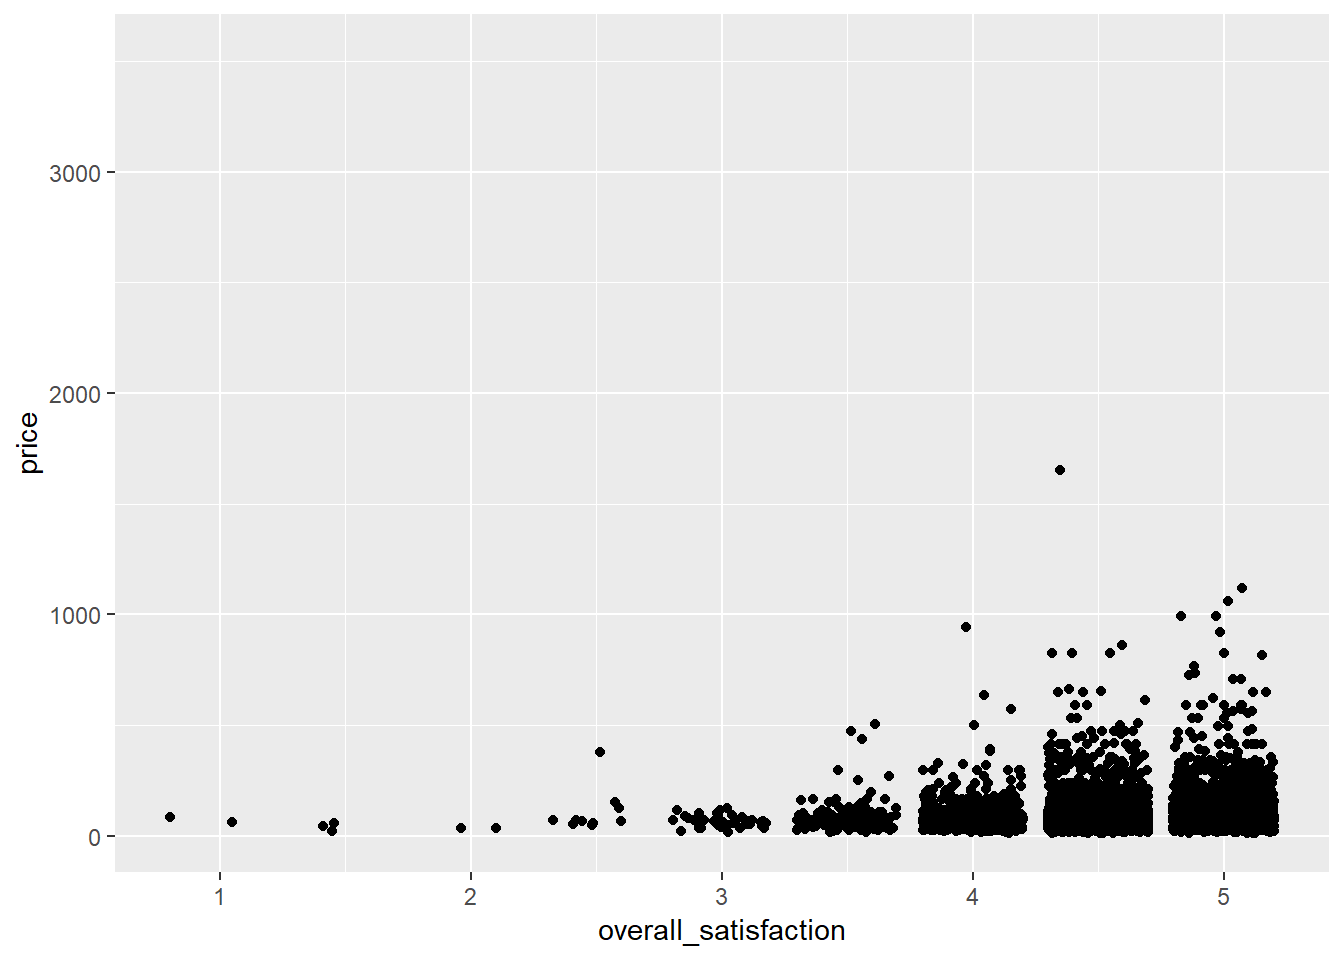
\includegraphics[width=12cm,height=8cm]{modelling_linreg_scatterplot-1.png} 
\end{center}

(Recebemos uma mensagem de erro informando que várias linhas foram removidas. Essas são as linhas com valores ausentes para a \fbox{overall\_satisfaction}, portanto, não há necessidade de se preocupar com essa mensagem de erro. Consulte as \href{https://bookdown.org/content/1340/data.html#modelling_manipulations}{manipulações de dados} para saber por que faltam valores para a \fbox{overall\_satisfaction}.)


Os outliers de preço reduzem a informatividade do gráfico, portanto, vamos transformar a variável \fbox{price}. Também vamos adicionar alguns meios ao gráfico, como aprendemos \href{https://bookdown.org/content/1340/graphs.html#graphs}{aqui}, e uma linha de regressão:

\begin{lstlisting}[language=R]
ggplot(data = airbnb, mapping = aes(x = overall_satisfaction, y = log(price, base = exp(1)))) +
  geom_jitter() + # jitter em vez de pontos, caso contrario, muitos pontos sao desenhados um sobre o outro
  stat_summary(fun.y=mean, colour="green", size = 4, geom="point", shape = 23, fill = "green") + # medias
  stat_smooth(method = "lm", se=FALSE) # reta de regressao
\end{lstlisting}

\begin{center}
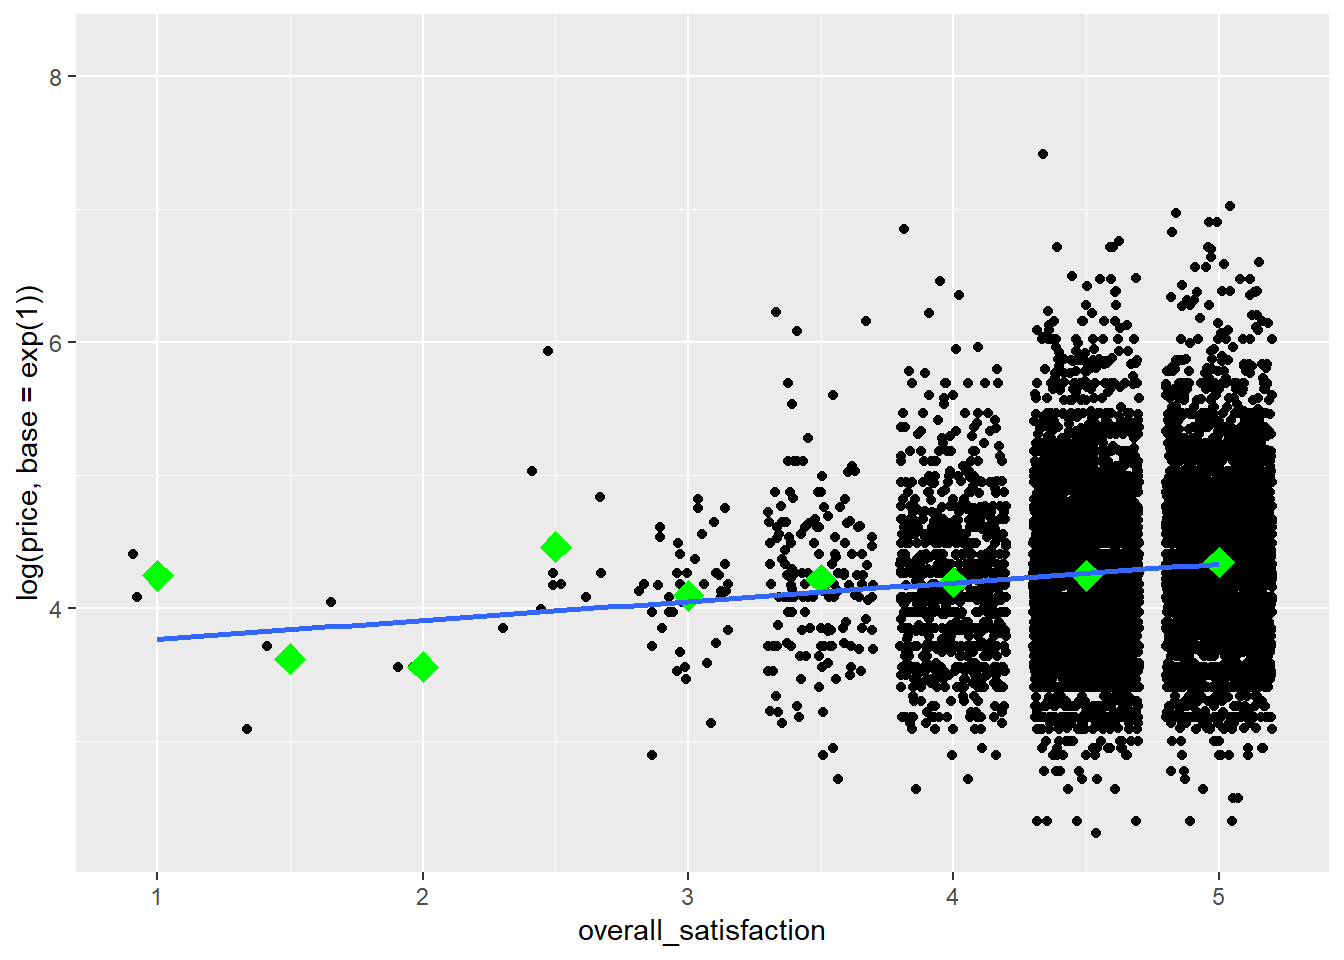
\includegraphics[width=12cm,height=8cm]{modelling_linreg_scatterplot_transformed-1.png} 
\end{center}

Vemos que o preço tende a aumentar um pouco com maior satisfação. Para testar se a relação entre preço e satisfação é realmente significativa, podemos realizar uma regressão simples (simples refere-se ao fato de haver apenas um preditor):


\begin{lstlisting}[language=R]
linearmodel <- lm(price ~ overall_satisfaction, data = airbnb) # criamos um modelo linear. O primeiro argumento eh o modelo que assume a forma de variavel dependente - variavel (s) independente (s). O segundo argumento sao os dados que devemos considerar.

summary(linearmodel) # solicite um resumo dos resultados desse modelo linear

## 
## Call:
## lm(formula = price ~ overall_satisfaction, data = airbnb)
## 
## Residuals:
##     Min      1Q  Median      3Q     Max 
##  -80.51  -38.33  -15.51   14.49 1564.67 
## 
## Coefficients:
##                      Estimate Std. Error t value Pr(>|t|)    
## (Intercept)            29.747      8.706   3.417 0.000636 ***
## overall_satisfaction   12.353      1.864   6.626 3.62e-11 ***
## ---
## Signif. codes:  0 '***' 0.001 '**' 0.01 '*' 0.05 '.' 0.1 ' ' 1
## 
## Residual standard error: 71.47 on 10585 degrees of freedom
##   (7064 observations deleted due to missingness)
## Multiple R-squared:  0.00413,    Adjusted R-squared:  0.004036 
## F-statistic:  43.9 on 1 and 10585 DF,  p-value: 3.619e-11
\end{lstlisting}

Vemos dois parâmetros neste modelo:

\begin{itemize}
    \item $\beta_{0}$ ou intercepto (29.75)
    \item $\beta_{1}$ inclinação de overral\_satisfaction (12.35)
\end{itemize}

Esses parâmetros têm as seguintes interpretações. A interceptação ($\beta_{0}$) é o preço estimado para uma observação com satisfação geral igual a zero. A inclinação ($\beta_{1}$) é o aumento estimado do preço para cada aumento na satisfação geral. Isso determina a inclinação da linha de regressão ajustada no gráfico. Portanto, para uma listagem com uma satisfação geral de, por exemplo, 3,5, o preço estimado é 29,75 + 3,5× 12,35 = 72,98.

A inclinação é positiva e significativa. Você pode relatar o seguinte: “Havia uma relação significativamente positiva entre preço e satisfação geral ($\beta = 12,35$, t (10585) = 6,63, $p <$0,001). "

Na saída, também obtemos informações sobre o modelo geral.

O modelo vem com um valor F de 43,9 com 1 grau de liberdade no numerador e 10585 graus de liberdade no denominador. Essa estatística F nos diz se nosso modelo com um preditor (\fbox{overall\_satisfaction}) prediz a variável dependente (\fbox{price}) melhor do que um modelo sem preditores (o que simplesmente preveria a média do preço para todos os níveis de satisfação geral). Os graus de liberdade nos permitem encontrar o valor $p$ correspondente ($<$0,001) da estatística F (43,9). Os graus de liberdade no numerador são iguais ao número de preditores em nosso modelo. Os graus de liberdade no denominador são iguais ao número de observações menos o número de preditores menos um. Lembre-se de que temos 10587 observações para as quais temos valores para \fbox{price} e \fbox{overall\_satisfaction}. Como o valor $p$ é menor que 0,05, rejeitamos a hipótese nula de que nosso modelo não prediz melhor a variável dependente do que um modelo sem preditores. Observe que, no caso de regressão linear simples, o valor p do modelo corresponde ao valor $p$ do preditor único. Para modelos com mais preditores, não existe essa correspondência.

Por fim, observe também a estatística do R quadrado do modelo. Esta estatística é igual a 0,004. Essa estatística nos diz quanto da variação na variável dependente é explicada por nossos preditores. Quanto mais preditores você adicionar a um modelo, maior será o R quadrado.


\subsection{Correlação}

Observe que na regressão linear simples, a inclinação do preditor é uma função da correlação entre o preditor e a variável dependente. Podemos calcular a correlação da seguinte maneira:

\begin{lstlisting}[language=R]
# Certifique-se de incluir o argumento use, caso contrario, o resultado sera NA devido aos valores ausentes na overall_satisfaction.
# O argumento use instrui o R para calcular a correlacao com base apenas nas observacoes para as quais temos dados sobre price e overall_satisfaction.

cor(airbnb$price, airbnb$overall_satisfaction, use = "pairwise.complete.obs")

## [1] 0.06426892
\end{lstlisting}

Vemos que a correlação é positiva, mas muito baixa (r = 0,064).

Elevando ao quadrado essa correlação, você obterá o R quadrado de um modelo com apenas esse preditor (0,064 × 0,064 = 0,004).

Ao lidar com múltiplos preditores (como na próxima seção), podemos gerar uma matriz de correlação. Isso é especialmente útil ao verificar a multicolinearidade. Digamos que desejamos que as correlações entre, \fbox{price}, \fbox{overall\_satisfaction}, \fbox{reviews}, \fbox{accommodates}:

\begin{lstlisting}[language=R]
airbnb.corr <- airbnb%>%
   filter(! is.na (overall_satisfaction))%>% # caso contrario, você vera NAs no resultado
   select(price, overall_satisfaction, reviews, accommodates)

cor(airbnb.corr) # obter a matriz de correlacao

cor(airbnb.corr) # obtenha a matriz de correlacao

##                            price overall_satisfaction     reviews
## price                 1.00000000           0.06426892 -0.05827489
## overall_satisfaction  0.06426892           1.00000000  0.03229339
## reviews              -0.05827489           0.03229339  1.00000000
## accommodates          0.63409855          -0.04698709 -0.03862767
##                      accommodates
## price                  0.63409855
## overall_satisfaction  -0.04698709
## reviews               -0.03862767
## accommodates           1.0000000
\end{lstlisting}

\newpage

Você pode visualizar facilmente essa matriz de correlação:

\begin{lstlisting}[language=R]
install.packages("corrplot") # instala e carrega o pacote corrplot
library(corrplot)

corrplot(cor(airbnb.corr), method = "number", type = "lower", bg = "grey") # apresente numa tabela
\end{lstlisting}


\begin{center}
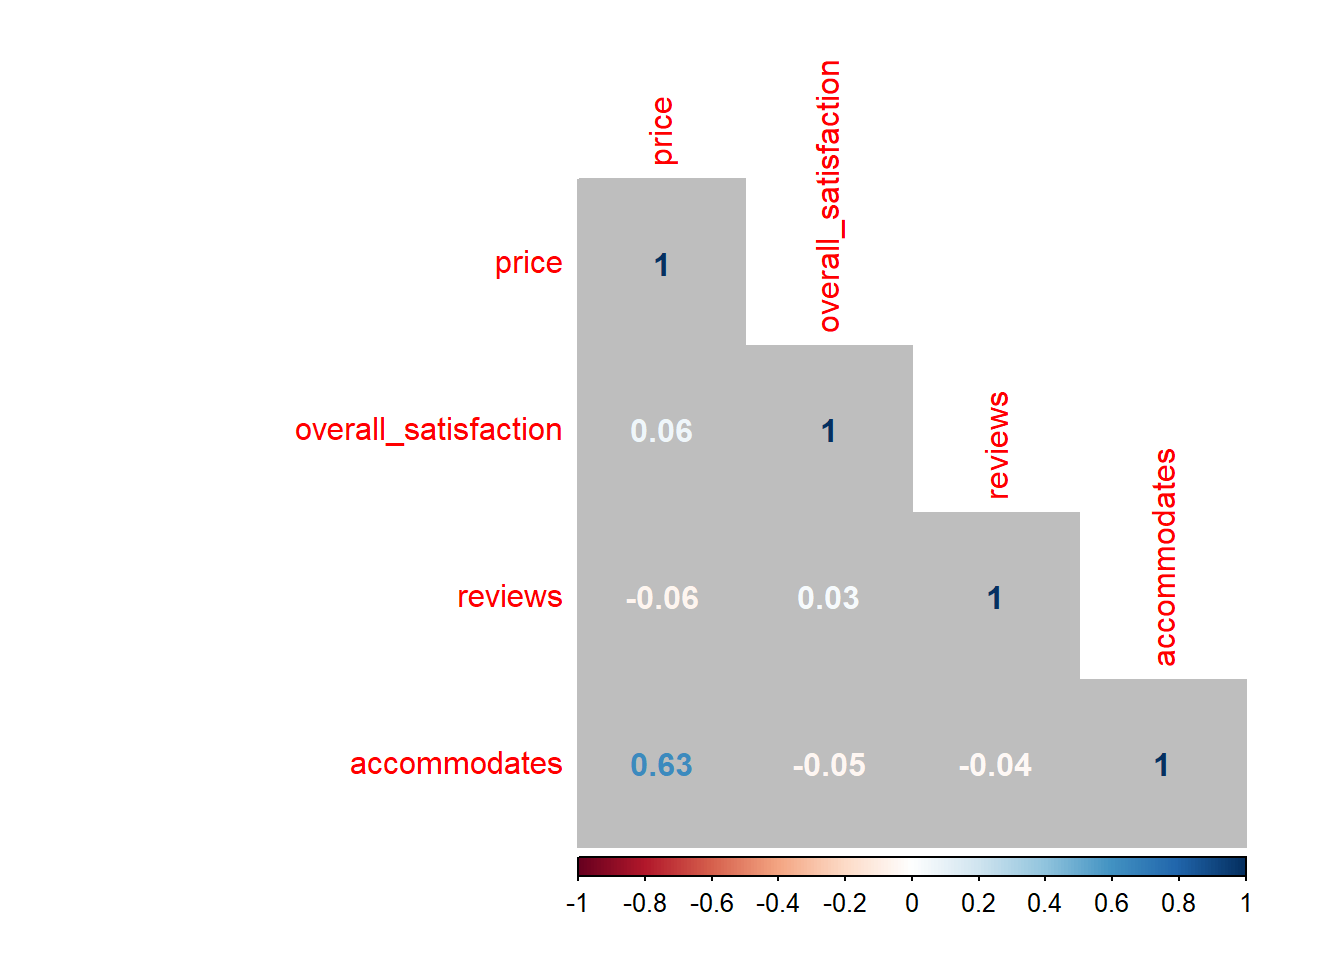
\includegraphics[width=12cm,height=8cm]{modelling_matrix2-1.png} 
\end{center}

As cores das correlações dependem de seus valores absolutos.

Você também pode obter valores de p para as correlações ($p <0,05$ indica que a correlação difere significativamente de zero):

\begin{lstlisting}[language=R]
# O comando para os valores-p eh cor.mtest(airbnb.corr)
# Mas queremos apenas os valores-p, portanto $ p
# E arredondamos para cinco digitos, portanto arredondamos (, 5)

round(cor.mtest(airbnb.corr)$p, 5) 
##      [,1]    [,2]    [,3]  [,4]
## [1,]    0 0.00000 0.00000 0e+00
## [2,]    0 0.00000 0.00089 0e+00
## [3,]    0 0.00089 0.00000 7e-05
## [4,]    0 0.00000 0.00007 0e+00
\end{lstlisting}

\newpage

\subsubsection{Regressão linear múltipla, com interação}

Frequentemente, estamos interessados em interações entre preditores (por exemplo, \fbox{overall\_satisfaction} e \fbox{reviews}). Uma interação entre preditores nos diz que o efeito de um preditor depende do nível do outro preditor:

\begin{lstlisting}[language=R]
# overall_satisfaction + reviews: a interacao nao eh incluida como preditor
# overall_satisfaction * reviews: a interacao entre os dois preditores eh incluida como preditora

## 
## Call:
## lm(formula = price ~ overall_satisfaction * reviews, data = airbnb)
## 
## Residuals:
##     Min      1Q  Median      3Q     Max 
##  -82.17  -36.71  -16.08   13.47 1561.53 
## 
## Coefficients:
##                              Estimate Std. Error t value Pr(>|t|)    
## (Intercept)                  48.77336   10.14434   4.808 1.55e-06 ***
## overall_satisfaction          8.91437    2.17246   4.103 4.10e-05 ***
## reviews                      -0.99200    0.26160  -3.792  0.00015 ***
## overall_satisfaction:reviews  0.18961    0.05573   3.402  0.00067 ***
## ---
## Signif. codes:  0 '***' 0.001 '**' 0.01 '*' 0.05 '.' 0.1 ' ' 1
## 
## Residual standard error: 71.31 on 10583 degrees of freedom
##   (7064 observations deleted due to missingness)
## Multiple R-squared:  0.008861,   Adjusted R-squared:  0.00858 
## F-statistic: 31.54 on 3 and 10583 DF,  p-value: < 2.2e-16

\end{lstlisting}

Com esse modelo, preço estimado = $\beta_{0} + \beta_{1}\mbox{\textit{overall\_satisfaction}} + \beta_{2}reviews + \beta_{3}\mbox{\textit{overall\_satisfaction}} × reviews$, em que:

\begin{itemize}
    \item $\beta_{0}$ é o intercepto (48.77)
    \item $\beta_{1}$ representa a relação entre overall\_satisfaction e price (8.91) controlando todas as outras variáveis em nosso modelo
    \item $\beta_{2}$ representa a relação entre revisões e preço (-0.99), controlando todas as outras variáveis em nosso modelo
    \item $\beta_{3}$ é a interação entre satisfação geral e revisões (0.19)
\end{itemize}

Para um determinado nível de reviews, o relacionamento entre overall\_satisfaction e price pode ser reescrito como:

$$
=[\beta_{0}+\beta_{2}reviews]+(\beta_{1}+\beta_{3}reviews)\times\,\,\mbox{\textit{overall\_satisfaction}}}
$$

Vemos que tanto a interceptação ($\beta_{0}+\beta_{2}reviews$) e a inclinação ($\beta_{1}+\beta_{3}reviews$) a relação entre \fbox{overall\_satisfaction} e \fbox{price} depende de \fbox{reviews}. No modelo sem interações, apenas a interceptação da relação entre \fbox{overall\_satisfaction} e \fbox{price} dependia de \fbox{reviews}. Como adicionamos ao nosso modelo uma interação entre a \fbox{overall\_satisfaction} e o \fbox{reviews}, a inclinação agora também depende de \fbox{reviews}.

Da mesma forma, para um determinado nível de \fbox{overall\_satisfaction}, o relacionamento entre \fbox{reviews} e \fbox{price} pode ser reescrito como:

$$
=[\beta_{0}+\beta_{1}\mbox{\textit{overall\_satisfaction}}]+(\beta_{2}+\beta_{3}\mbox{\textit{overall\_satisfaction}})\times\,\,reviews
$$

Aqui também vemos que tanto a interceptação quanto a inclinação da relação entre revisões (\fbox{reviews}) e preço (\fbox{price}) dependem da satisfação geral (\fbox{overall\_satisfaction}).

Como dito, quando o relacionamento entre uma variável independente e uma variável dependente depende do nível de outra variável independente, temos uma interação entre as duas variáveis independentes. Para esses dados, a interação é altamente significativa ($p <0,001$). Vamos visualizar essa interação. Nós nos concentramos na relação entre satisfação geral e preço. Planejaremos isso para um nível de comentários que possa ser considerado baixo, médio e alto:

\begin{lstlisting}[language=R]
airbnb %>% 
  filter(!is.na(overall_satisfaction)) %>% 
  summarize(min = min(reviews),
            Q1 = quantile(reviews, .25), # primeiro quartil
            Q2 = quantile(reviews, .50), # segundo quartil ou mediana
            Q3 = quantile(reviews, .75), # terceiro quartil
            max = max(reviews),
            mean = mean(reviews))
            
## # A tibble: 1 x 6
##     min    Q1    Q2    Q3   max  mean
##   <dbl> <dbl> <dbl> <dbl> <dbl> <dbl>
## 1     3     6    13    32   708  28.5
\end{lstlisting}


Vimos que 25\% das listagens têm 6 ou menos comentários, 50\% das listagens tem 13 ou menos comentários e 75\% das listagens tem 32 ou menos comentários.

Queremos três grupos, no entanto, para que possamos pedir quantis diferentes:

\begin{lstlisting}[language=R]
airbnb %>% 
  filter(!is.na(overall_satisfaction)) %>% 
  summarize(Q1 = quantile(reviews, .33), # baixo
            Q2 = quantile(reviews, .66), # medio
            max = max(reviews))          # alto
            
## # A tibble: 1 x 3
##      Q1    Q2   max
##   <dbl> <dbl> <dbl>
## 1     8    23   708
\end{lstlisting}

e crie grupos com base nesses números:

\begin{lstlisting}[language=R]
airbnb.reviews <- airbnb %>% 
  filter(!is.na(overall_satisfaction)) %>% 
  mutate(review_group = case_when(reviews <= quantile(reviews, .33) ~ "low",
                                  reviews <= quantile(reviews, .66) ~ "medium",
                                  TRUE                              ~ "high"),
         review_group = factor(review_group, levels = c("low","medium","high")))
\end{lstlisting}

Por isso, pedimos ao \faRProject para criar uma nova variável \fbox{review\_group} que deve ser igual a "low" quando o número de revisões for menor ou igual ao 33º percentil, "medium" quando o número de revisões for menor ou igual ao 66º percentil e "high", caso contrário. Depois, fatoramos a variável \fbox{review\_group} recém-criada e fornecemos um novo argumento, \fbox{levels}, que especifica a ordem dos níveis dos fatores (caso contrário, a ordem seria alfabética: alta, baixa, média). Vamos verificar se o agrupamento foi bem-sucedido:

\begin{lstlisting}[language=R]
# checagem:
airbnb.reviews %>% 
  group_by(review_group) %>% 
  summarize(min = min(reviews), max = max(reviews))
  
## # A tibble: 3 x 3
##   review_group   min   max
##   <fct>        <dbl> <dbl>
## 1 low              3     8
## 2 medium           9    23
## 3 high            24   708
\end{lstlisting}

De fato, o número máximo de revisões em cada grupo corresponde aos pontos de corte definidos acima. Agora, podemos solicitar a \faRProject um gráfico da relação entre \fbox{overall\_satisfaction} e \fbox{price} para os três níveis de revisão:

\begin{lstlisting}[language=R]
ggplot(data = airbnb.reviews, mapping = aes(x = overall_satisfaction, y = log(price, base = exp(1)))) + # transformacao log de preco
  facet_wrap(~ review_group) + # peca paineis diferentes para cada grupo de revisao
  geom_jitter() +
  stat_smooth(method = "lm", se = FALSE)
\end{lstlisting}

\begin{center}
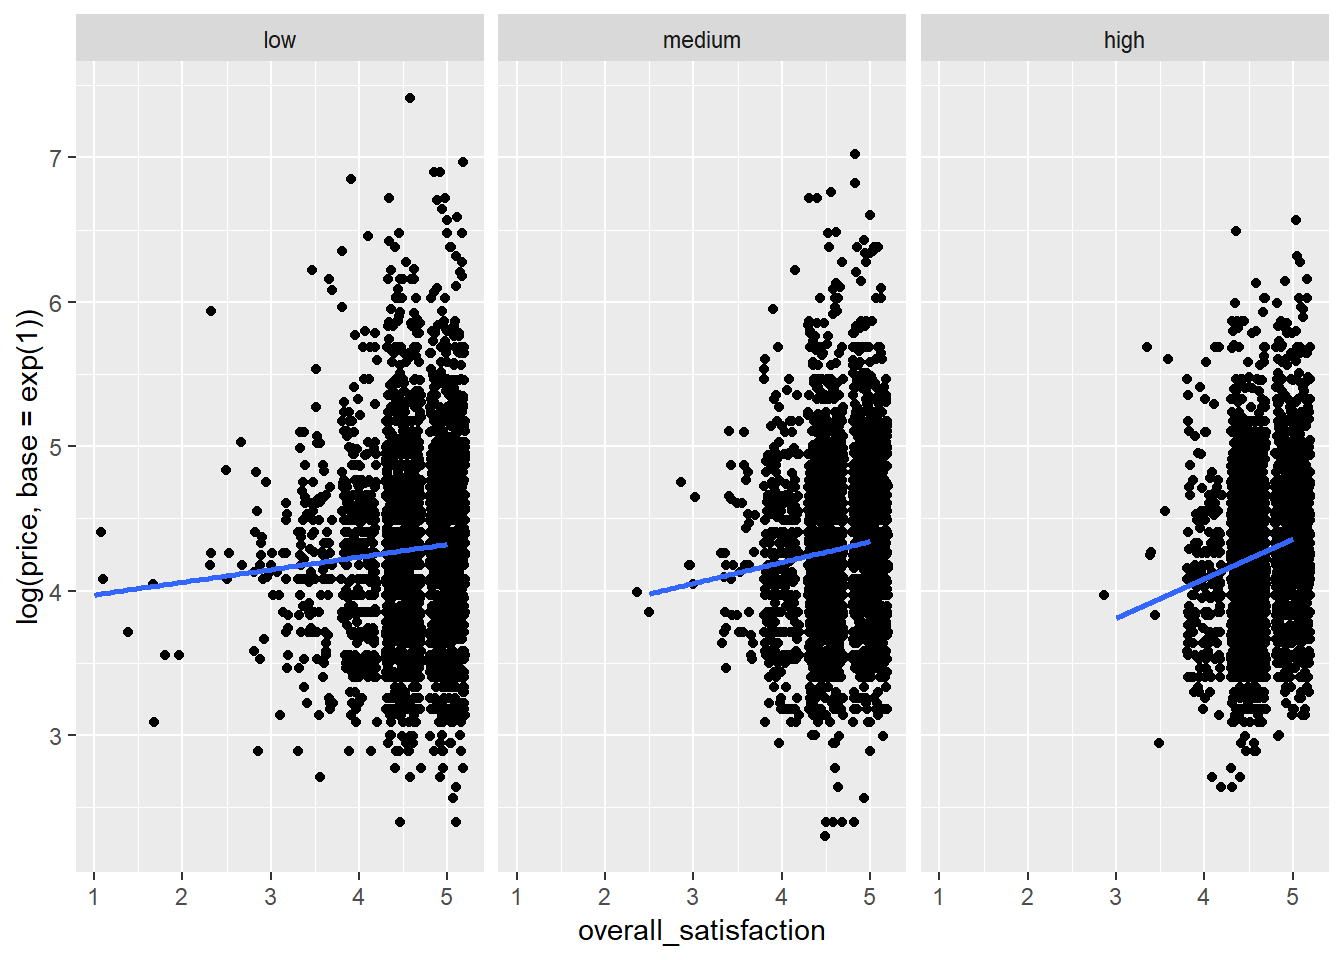
\includegraphics[width=12cm,height=8cm]{modelling_multiple_linreg_groups_plot-1.png} 
\end{center}

Vemos que a relação entre \fbox{overall\_satisfaction} e \fbox{price} é sempre positiva, mas é mais positiva para listagens com muitas críticas do que para listagens com poucas críticas. Pode haver muitas razões para isso. Talvez seja o caso de listagens com críticas positivas aumentarem o preço, mas somente depois de receberem uma certa quantidade de críticas.

Também vemos que as listagens com muitas avaliações quase nunca têm uma classificação de satisfação menor que 3. Isso faz sentido, porque é difícil continuar atraindo pessoas quando a classificação de uma listagem é baixa. Listas com poucas críticas tendem a ter baixos índices de satisfação geral.

Portanto, parece que nossos preditores estão correlacionados: quanto mais avaliações uma listagem tiver, maior será seu índice de satisfação. Isso potencialmente apresenta um problema que discutiremos em uma das próximas seções sobre \href{https://bookdown.org/content/1340/linear-regression.html#multicollinearity}{multicolinearidade.}

\subsubsection{Premissas}

Antes de tirar conclusões de uma análise de regressão, é preciso verificar várias suposições. Essas premissas devem ser atendidas independentemente do número de preditores no modelo, mas continuaremos com o caso de dois preditores.

\subsubsubsection{Normalidade dos resíduos}

Os resíduos (a diferença entre os valores observados e os estimados) devem ser normalmente distribuídos. Podemos inspecionar visualmente os resíduos:

\begin{lstlisting}[language=R]
linearmodel <- lm(price ~ overall_satisfaction * reviews, data = airbnb)
residuals <- as_tibble(resid(linearmodel))  

Atenção: Chamar `as_tibble ()` em um vetor é desencorajado, porque é provável que o comportamento mude no futuro. Use `enframe (name = NULL)` em seu lugar.
## Este aviso é exibido uma vez por sessão.

# veja os residuos do modelo linear com resid(linearmodel) 
# e mude isso em seu dataframe com as_tibble()

ggplot(data = residuals, mapping = aes(x = value)) + 
  geom_histogram()
  
## `stat_bin()` usando `bins = 30`. Obtenha um valor melhor com `binwidth`.
\end{lstlisting}



\begin{center}
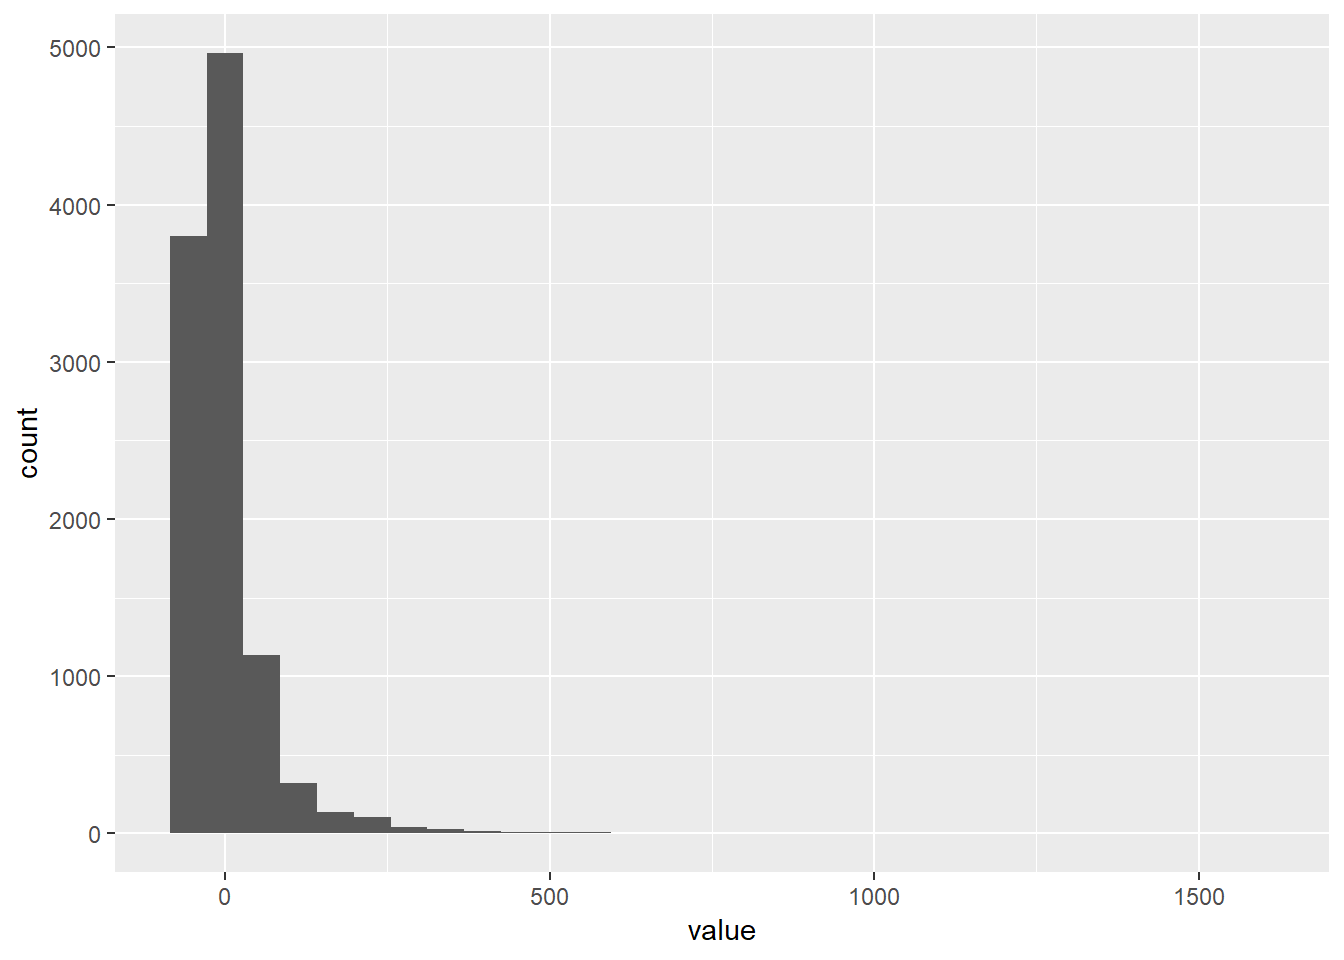
\includegraphics[width=12cm,height=8cm]{modelling_normality-1.png} 
\end{center}

\vspace{.25cm}

\subsubsubsection{\textbf{Homocedasticidade dos resíduos}}

\vspace{.25cm}

Os resíduos (a diferença entre os valores observados e os estimados) devem ter uma variação constante. Podemos verificar isso plotando os resíduos versus os valores previstos:

\begin{lstlisting}[language=R]
linearmodel <- lm(price ~ overall_satisfaction * reviews, data = airbnb)

 # cria um dataframe (a tibble)
residuals_predicted <- tibble(residuals = resid(linearmodel), # a primeira variavel são residuos, que sao os residuos do nosso modelo linear
                              predicted = predict(linearmodel)) # a segunda variavel eh prevista, quais sao os valores previstos do nosso modelo linear

ggplot(data = residuals_predicted, mapping = aes(x = predicted, y = residuals)) + 
  geom_point()
\end{lstlisting}

\begin{center}
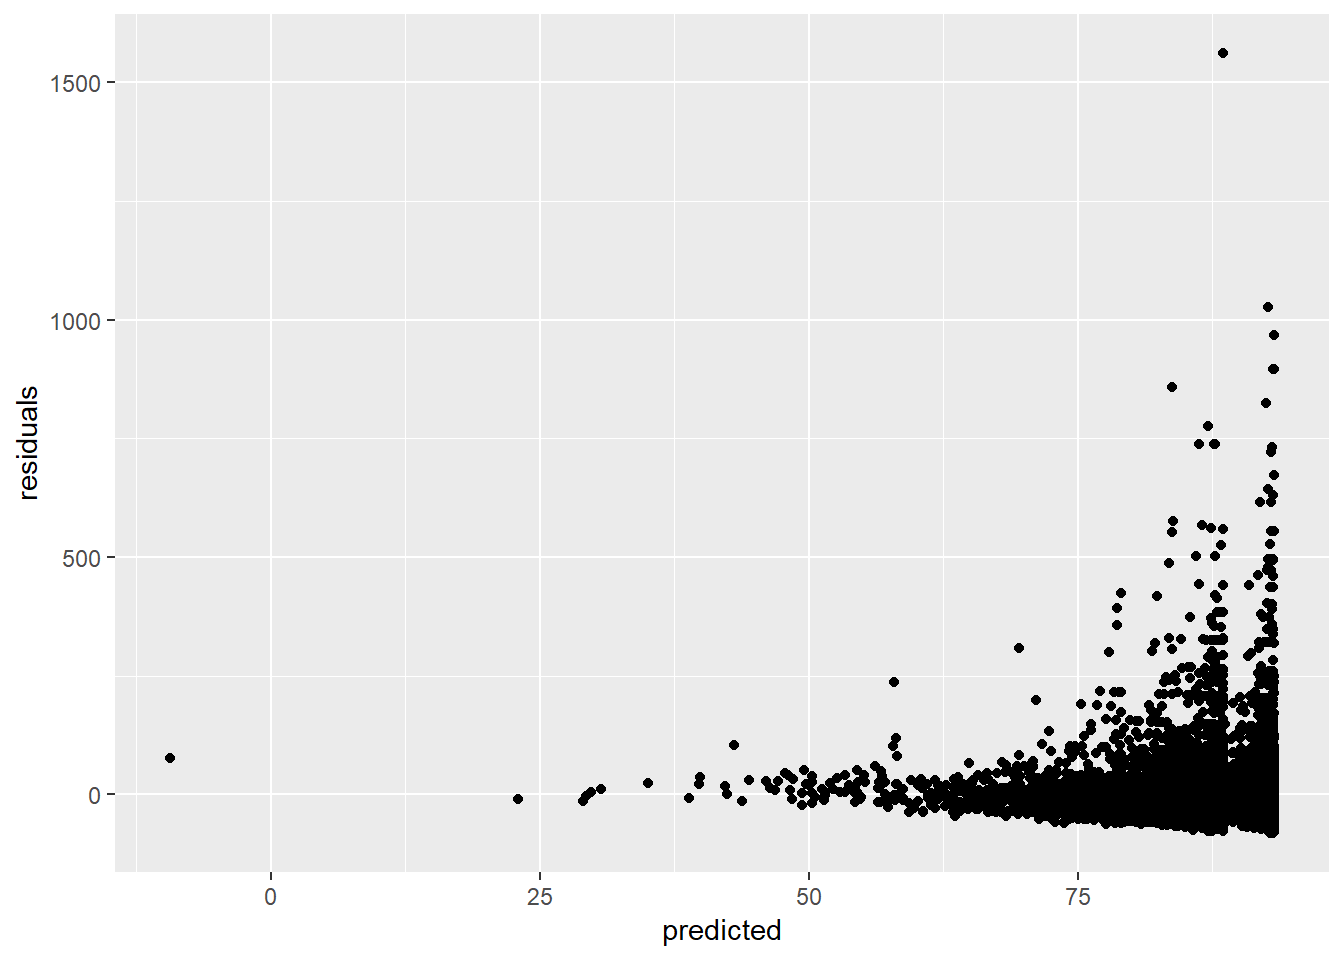
\includegraphics[width=12cm,height=8cm]{modelling_homoscedasticity-1.png} 
\end{center}

Essa suposição é violada porque, quanto maiores nossos valores previstos, maior a variação que vemos nos resíduos.

\newpage

\subsubsubsection{\textbf{Multicolinearidade}}

\vspace{.25cm}

A multicolinearidade existe sempre que dois ou mais dos preditores em um modelo de regressão são moderadamente ou altamente correlacionados (portanto, é claro que isso não é um problema no caso de regressão simples). Vamos testar a correlação entre \fbox{overall\_satisfaction} e \fbox{reviews}:

\begin{lstlisting}[language=R]
# Certifique-se de incluir o argumento use, caso contrario, o resultado sera NA devido aos valores ausentes no overall_satisfaction.
# O argumento use instrui o R para calcular a correlacao com base apenas nas observacoes para as quais temos dados sobre price e overall_satisfaction.

cor.test(airbnb$overall_satisfaction,airbnb$reviews, use = "pairwise.complete.obs") # teste para correlacao

## 
##  Pearson's product-moment correlation
## 
## data:  airbnb$overall_satisfaction and airbnb$reviews
## t = 3.3242, df = 10585, p-value = 0.0008898
## alternative hypothesis: true correlation is not equal to 0
## 95 percent confidence interval:
##  0.01325261 0.05131076
## sample estimates:
##        cor 
## 0.03229339
\end{lstlisting}

Nossos preditores são de fato significativamente correlacionados ($p <$0,001), mas a correlação é realmente baixa (0,03). Ao lidar com mais de dois preditores, é uma boa idéia criar uma matriz de correlação.

O problema da multicolinearidade é que ela infla os erros padrão dos coeficientes de regressão. Como resultado, os testes de significância desses coeficientes terão mais dificuldade em rejeitar a hipótese nula. Podemos facilmente ter uma idéia do grau em que os coeficientes são inflados. Para ilustrar isso, vamos estimar um modelo com preditores correlacionados: acomodações (\fbox{accommodates}) e preço (\fbox{price}) ($r = 0,56$).

\begin{lstlisting}[language=R]
linearmodel <- lm(overall_satisfaction ~  accommodates * price, data = airbnb)
summary(linearmodel)

## 
## Call:
## lm(formula = overall_satisfaction ~ accommodates * price, data = airbnb)
## 
## Residuals:
##     Min      1Q  Median      3Q     Max 
## -3.6494 -0.1624 -0.1105  0.3363  0.6022 
## 
## Coefficients:
##                      Estimate Std. Error t value Pr(>|t|)    
## (Intercept)         4.622e+00  9.938e-03 465.031  < 2e-16 ***
## accommodates       -1.640e-02  2.039e-03  -8.046 9.48e-16 ***
## price               1.356e-03  1.159e-04  11.702  < 2e-16 ***
## accommodates:price -5.423e-05  9.694e-06  -5.595 2.26e-08 ***
## ---
## Signif. codes:  0 '***' 0.001 '**' 0.01 '*' 0.05 '.' 0.1 ' ' 1
## 
## Residual standard error: 0.3689 on 10583 degrees of freedom
##   (7064 observations deleted due to missingness)
## Multiple R-squared:  0.0199, Adjusted R-squared:  0.01963 
## F-statistic: 71.64 on 3 and 10583 DF,  p-value: < 2.2e-16
\end{lstlisting}

Vemos que todos os preditores são significativos. Vamos dar uma olhada nos fatores de inflação da variância:

\begin{lstlisting}[language=R]
library(car) # a funcao vif eh do pacote cars

vif(linearmodel)

##       accommodates              price accommodates:price 
##           2.090206           5.359203           6.678312
\end{lstlisting}

Os fatores VIF informam até que ponto os erros padrão são inflados. Uma regra prática é que VIFs de 5 e acima indicam inflação significativa.

\subsection{Teste qui-quadrado}

Suponha que tenhamos interesse em encontrar uma verdadeira jóia (\fbox{gem}) de uma lista. Por exemplo, estamos interessados em listagens com uma classificação de 5 em 5 e pelo menos 30 avaliações:

\begin{lstlisting}[language=R]
airbnb <- airbnb %>% 
  mutate(gem = (overall_satisfaction == 5 & reviews>=30), # duas condicoes devem ser atendidas antes de dizer que uma listagem eh uma joia
         gem = factor(gem, labels = c("no gem","gem")))  # dê à variável lógica rótulos mais intuitivos
\end{lstlisting}

Agora, digamos que estamos interessados em saber se é mais provável encontrar "jóias" (\fbox{gem}) em cidades pequenas ou grandes (criamos a variável de tamanho aqui). O teste do qui-quadrado pode fornecer uma resposta a essa pergunta testando a hipótese nula de não haver relação entre duas variáveis categóricas (tamanho da cidade:  \fbox{large} vs. \fbox{small} & \fbox{gem}: \fbox{yes} vs. \fbox{no}). 

Ele compara a tabela de frequências observada com a tabela de frequências que você esperaria quando não houvesse relação entre as duas variáveis. Quanto mais as tabelas de frequência observada e esperada divergem, maior a estatística qui-quadrado, menor o valor de p e menos provável é que as duas variáveis não sejam relacionadas.

Antes de realizarmos um teste qui-quadrado, lembre-se de que algumas cidades têm um valor em falta para o tamanho porque têm um valor em falta para a \fbox{population}. Vamos filtrar isso primeiro:

\begin{lstlisting}[language=R]
airbnb.cities <- airbnb %>% 
  filter(!is.na(size)) 

# queremos apenas aquelas observacoes em que tamanho nao eh NA. ! significa 'nao'
# veja https://r4ds.had.co.nz/transform.html#filter-rows-with-filter para mais funcoes logicas (desca ate a secao 5.2.2)
\end{lstlisting}

Agora, imprima as frequências do tamanho da cidade e combinações de gems:

\begin{lstlisting}[language=R]
airbnb.cities %>% 
  group_by(size, gem) %>% 
  summarize(count = n())
  
## # A tibble: 4 x 3
## # Groups:   size [?]
##   size  gem    count
##   <fct> <fct>  <int>
## 1 small no gem  4095
## 2 small gem      175
## 3 large no gem 10755
## 4 large gem      941
\end{lstlisting}

Esta informação está correta, mas o formato em que a tabela é apresentada é um pouco incomum. Gostaríamos de ter uma variável como linhas e a outra como colunas:

\begin{lstlisting}[language=R]
table(airbnb.cities$size, airbnb.cities$gem)

##        
##         no gem   gem
##   small   4095   175
##   large  10755   941
\end{lstlisting}


Isso é um pouco mais fácil de interpretar. Uma tabela como essa é frequentemente chamada de tabela cruzada. É fácil pedir porcentagens em vez de contagens:

\begin{lstlisting}[language=R]
crosstable <- table(airbnb.cities$size, airbnb.cities$gem) #Precisamos salvar a tabela cruzada primeiro.

prop.table(crosstable) # Use a funcao prop.table () para solicitar porcentagens.

##        
##             no gem        gem
##   small 0.25648253 0.01096079
##   large 0.67361894 0.05893774
prop.table(crosstable,1) # This gives percentages conditional on rows, i.e., the percentages in the rows sum to 1.
##        
##             no gem        gem
##   small 0.95901639 0.04098361
##   large 0.91954514 0.08045486
prop.table(crosstable,2) # This gives percentages conditional on columns, i.e., the percentages in the columns sum to 1.
##        
##            no gem       gem
##   small 0.2757576 0.1568100
##   large 0.7242424 0.8431900
\end{lstlisting}

Com base nessas frequências ou porcentagens, não devemos esperar uma forte relação entre \fbox{size} e \fbox{gem}. Vamos realizar o teste do qui-quadrado para testar nossa intuição:

\begin{lstlisting}[language=R]
chisq.test(crosstable)

## 
##  Pearson's Chi-squared test with Yates' continuity correction
## 
## data:  crosstable
## X-squared = 74.355, df = 1, p-value < 2.2e-16
\end{lstlisting}

O valor da estatística qui é 74,35 e o valor p é praticamente 0, por isso rejeitamos a hipótese nula de nenhum relacionamento. Não é o que esperávamos, mas o valor p é baixo porque nossa amostra é bastante grande (15966 observações). 

Você pode relatar o seguinte: “Havia uma relação significativa entre o tamanho da cidade e se uma listagem era ou não uma jóia ($\chi^{2} (1, N = 15966) = 74,35, p <0,001$), de modo que as cidades grandes (8,05\%) tinham uma porcentagem maior de jóias (raridades) do que as cidades pequenas (4,1\%). 

\subsection{Regressão logística (opcional)}

Às vezes, queremos prever uma variável dependente binária, ou seja, uma variável que pode assumir apenas dois valores, com base em várias variáveis independentes contínuas ou categóricas. Por exemplo, digamos que estamos interessados em testar se uma listagem é ou não uma jóia depende do preço e do tipo de quarto da listagem.

Não podemos usar ANOVA ou regressão linear aqui porque a variável dependente é uma variável binária e, portanto, normalmente não é distribuída. Outro problema com a ANOVA ou regressão linear é que ela pode prever valores que não são possíveis (por exemplo, nosso valor previsto pode ser 5, mas apenas 0 e 1 fazem sentido para essa variável dependente). Portanto, usaremos regressão logística. A regressão logística primeiro transforma a variável dependente Y com a transformação do logit. A transformação do logit usa o logaritmo natural das chances de que a variável dependente seja igual a 1:
\vspace{.25cm}

$$
probabilidades=\displaystyle\frac{P(Y=1)}{P(Y=0}=\displaystyle\frac{P(Y=1)}{1-P(Y=1)}
$$

\vspace{.25cm}
\hspace{5cm}então o logit $P(Y=1))=\ln\displaystyle\frac{P(Y-1)}{1-P(Y=1)}$
\vspace{.25cm}

Isso garante que nossa variável dependente seja normalmente distribuída e não seja restrita a ser 0 ou 1.

Vamos realizar a regressão logística:

\begin{lstlisting}[language=R]
logistic.model <- glm(gem ~ price * room_type, data=airbnb, family="binomial") # o argumento family = "binomial" diz R para tratar a variavel dependente como uma variavel 0/1
summary(logistic.model) # saida da regressao

## 
## Call:
## glm(formula = gem ~ price * room_type, family = "binomial", data = airbnb)
## 
## Deviance Residuals: 
##     Min       1Q   Median       3Q      Max  
## -0.4909  -0.3819  -0.3756  -0.3660   2.5307  
## 
## Coefficients:
##                               Estimate Std. Error z value Pr(>|z|)    
## (Intercept)                 -2.5270702  0.0570207 -44.318   <2e-16 ***
## price                       -0.0007185  0.0004030  -1.783   0.0746 .  
## room_typePrivate room       -0.0334362  0.1072091  -0.312   0.7551    
## room_typeShared room         1.0986318  1.1278159   0.974   0.3300    
## price:room_typePrivate room -0.0011336  0.0012941  -0.876   0.3810    
## price:room_typeShared room  -0.0562610  0.0381846  -1.473   0.1406    
## ---
## Signif. codes:  0 '***' 0.001 '**' 0.01 '*' 0.05 '.' 0.1 ' ' 1
## 
## (Dispersion parameter for binomial family taken to be 1)
## 
##     Null deviance: 8663.8  on 17650  degrees of freedom
## Residual deviance: 8648.6  on 17645  degrees of freedom
## AIC: 8660.6
## 
## Number of Fisher Scoring iterations: 7

\end{lstlisting}


Vemos que o único preditor marginalmente significativo de uma listagem ser ou não uma jóia é o preço da listagem. Você pode relatar o seguinte: “Controlando o tipo de quarto e a interação entre preço e tipo de quarto, havia uma relação negativa marginalmente significativa entre o preço e a probabilidade de uma listagem ser uma jóia ($\beta$ = -0.0007185, $\chi$ (17645) = -1,783, p = 0,075). 

A interpretação dos coeficientes de regressão na regressão logística é diferente da do caso da regressão linear:

\begin{lstlisting}[language=R]
summary(logistic.model)
## 
## Call:
## glm(formula = gem ~ price * room_type, family = "binomial", data = airbnb)
## 
## Deviance Residuals: 
##     Min       1Q   Median       3Q      Max  
## -0.4909  -0.3819  -0.3756  -0.3660   2.5307  
## 
## Coefficients:
##                               Estimate Std. Error z value Pr(>|z|)    
## (Intercept)                 -2.5270702  0.0570207 -44.318   <2e-16 ***
## price                       -0.0007185  0.0004030  -1.783   0.0746 .  
## room_typePrivate room       -0.0334362  0.1072091  -0.312   0.7551    
## room_typeShared room         1.0986318  1.1278159   0.974   0.3300    
## price:room_typePrivate room -0.0011336  0.0012941  -0.876   0.3810    
## price:room_typeShared room  -0.0562610  0.0381846  -1.473   0.1406    
## ---
## Signif. codes:  0 '***' 0.001 '**' 0.01 '*' 0.05 '.' 0.1 ' ' 1
## 
## (Dispersion parameter for binomial family taken to be 1)
## 
##     Null deviance: 8663.8  on 17650  degrees of freedom
## Residual deviance: 8648.6  on 17645  degrees of freedom
## AIC: 8660.6
## 
## Number of Fisher Scoring iterations: 7

\end{lstlisting}

O coeficiente de regressão do preço é -0.0007185. Isso significa que um aumento de uma unidade no preço levará a um aumento de -0.0007185 nas chances de log de joia ser igual a 1 (ou seja, de uma listagem sendo uma joia). Por exemplo:

\begin{align}
    
\textrm{logit}(P(Y &= 1 | \textrm{price} = 60 )) = \textrm{logit}(P(Y = 1 | \textrm{price} = 59 )) - 0.0007185\\

\vspace{.25cm}

\Leftrightarrow \textrm{logit}(P(Y = 1 | \textrm{price} = 60 )) - \textrm{logit}(P(Y &= 1 | \textrm{price} = 59 )) = -0.0007185\\

\vspace{.25cm}

\Leftrightarrow \textrm{ln(probabilidades}(P(Y = 1 | \textrm{price} = 60 )) - \textrm{ln(probabilidades}(P(Y &= 1 | \textrm{price} = 59 )) = -0.0007185\\

\vspace{.25cm}

\Leftrightarrow \textrm{ln}(\dfrac{ \textrm{probabilidades}(P(Y = 1 | \textrm{price} &= 60 )}{\textrm{probabilidades}(P(Y = 1 | \textrm{price} = 59 )}) = -0.0007185\\

\vspace{.25cm}

\Leftrightarrow \dfrac{ \textrm{probabilidades}(P(Y = 1 | \textrm{price} = 60 )}{\textrm{probabilidades}(P(Y &= 1 | \textrm{price} = 59 )} = e^{-0.0007185}\\

\vspace{.25cm}

\Leftrightarrow \textrm{probabilidades}(P(Y &= 1 | \textrm{price} = 60 ) = e^{-0.0007185} * \textrm{probabilidades}(P(Y &= 1 | \textrm{price} = 59 ))
\end{align}


Assim, o coeficiente de regressão em uma regressão logística deve ser interpretado como o aumento relativo nas chances da variável dependente ser igual a 1, para cada aumento de unidade no preditor, controlando todos os outros fatores em nosso modelo. Nesse caso, as probabilidades de uma listagem ser uma gema devem ser multiplicadas por $ e ^ {0,0007185} = 0,999 $ ou diminuídas em 0,1\%, para cada aumento de preço unitário. Em outras palavras, listagens mais caras têm menos probabilidade de serem jóias. No exemplo específico acima, as chances de ser uma joia de uma listagem com preço de 60 são $e^{(-0.0007185×5)}= 0,996$ vezes a chance de ser uma jóia de uma listagem com preço de 59.

\subsubsection{Medindo o ajuste de uma regressão logística: porcentagem classificada corretamente}

Nosso modelo usa o preço e o tipo de quarto da listagem para prever se a listagem é uma joia ou não. Ao fazer previsões, é natural nos perguntarmos se nossas previsões são boas. Em outras palavras, usando preço e tipo de quarto, com que frequência prevemos corretamente se uma listagem é uma jóia ou não? Para ter uma idéia da qualidade de nossas previsões, podemos pegar o preço e o tipo de quarto das listagens em nosso conjunto de dados, prever se as listagens são gemas e comparar nossas previsões com o status real da gema das listagens. Vamos primeiro fazer as previsões:

\begin{lstlisting}[language=R]
airbnb <- airbnb %>% 
  mutate(prediction = predict(logistic.model, airbnb))
# Crie uma nova coluna chamada previsao no quadro de dados do airbnb e armazene nela a previsao,
# baseado em logistic.model, para os dados do airbnb
# De uma olhada nessas previsoes:
head (previsão de airbnb $)
## 1 2 3 4 5 6
## -4.790232 -4.448355 -4.049498 -4.619293 -4.106477 -4.847211
# Compare com as observacoes:
head(airbnb$gem)
## [1] no gem no gem no gem no gem no gem no gem
## Levels: no gem gem
\end{lstlisting}

Você vê o problema? As previsões são logits, ou seja, logaritmos de chances de que as listagens sejam gemas, mas as observações simplesmente nos dizem se uma listagem é uma gema ou não. Para uma comparação significativa entre previsões e observações, precisamos transformar os logits em uma decisão: gema ou não gema. É fácil transformar logits em probabilidades usando o exponencial do logit. A relação entre probabilidades e probabilidades é a seguinte:

\vspace{.5cm}
\begin{center}
    $\textrm{probabilidades} = \dfrac{P(Y = 1)}{P(Y = 0)} = \dfrac{P(Y = 1)}{1 - P(Y = 1)})$\\
 
\vspace{.5cm}

    $\Leftrightarrow \dfrac{probabilidades}{1 + \dfrac{P(Y &= 1)}{1 - P(Y = 1)}} = \dfrac{\dfrac{P(Y = 1)}{1 - P(Y = 1)}}{1 + \dfrac{P(Y = 1)}{1 - P(Y = 1)}})$\\

\vspace{.5cm}    
    $\Leftrightarrow \dfrac{probabilidades}{1 + probabilidades} = \dfrac{\dfrac{P(Y = 1)}{1 - P(Y = 1)}}{\dfrac{1 - P(Y = 1) + P(Y = 1)}{1 - P(Y = 1)}})$\\
    
\vspace{.5cm}    
    $\Leftrightarrow \dfrac{probabilidades}{1 + probabilidades} = \dfrac{P(Y = 1)}{1 - P(Y = 1) + P(Y = 1)})\\$
    
\vspace{.5cm}    
    $\Leftrightarrow \dfrac{probabilidades}{1 + probabilidades} = P(Y = 1))$
\end{center}
 

Agora vamos calcular, para cada listagem, a probabilidade de a listagem ser uma jóia (\fbox{gem}):

\begin{lstlisting}[language=R]
airbnb <- airbnb %>% 
  mutate(prediction.logit = predict(logistic.model, airbnb),
         prediction.odds = exp(prediction.logit),
         prediction.probability = prediction.odds / (1+prediction.odds))

# Inspecionando as probabilidades preditas
head(airbnb$prediction.probability)

##           1           2           3           4           5           6 
## 0.008242034 0.011562542 0.017132489 0.009763496 0.016198950 0.007789092
\end{lstlisting}

Os primeiros números são probabilidades muito baixas, mas também existem probabilidades mais altas e todas as previsões estão entre 0 e 1, como deveriam. Agora precisamos decidir qual probabilidade é suficiente para prevermos que uma listagem é uma \fbox{gem} ou não. 


Uma escolha óbvia é uma probabilidade de 0,5: uma probabilidade maior que 0,5 significa que prevemos que é mais provável que uma listagem seja uma \fbox{gem} do que não. Vamos converter probabilidades em previsões:

\begin{lstlisting}[language=R]
airbnb <- airbnb %>% 
  mutate(prediction = case_when(prediction.probability<=.50 ~ "no gem",
                                prediction.probability> .50 ~ "gem"))

# Inspecinando as predicoes
head(airbnb$prediction)
## [1] "no gem" "no gem" "no gem" "no gem" "no gem" "no gem"

\end{lstlisting}

Uma etapa final é comparar previsões com observações:

\begin{lstlisting}[language=R]
table(airbnb$prediction, airbnb$gem)
##         
##          no gem   gem
##   no gem  16471  1180
\end{lstlisting}

Normalmente, vemos uma tabela 2x2, mas vemos uma tabela com um valor previsto nas linhas e dois valores observados nas colunas. Isso ocorre porque todas as probabilidades previstas estão abaixo de 0,50 e, portanto, sempre previmos que não há gemas. Vamos reduzir o limite para prever que uma listagem é uma \fbox{gem}:

\begin{lstlisting}[language=R]
airbnb <- airbnb %>% 
  mutate(prediction = case_when(prediction.probability<=.07 ~ "no gem",
                                prediction.probability> .07 ~ "gem"),
         prediction = factor(prediction, levels = c("no gem","gem")))# verifique se nenhuma joia eh o primeiro nivel do nosso fator

# Observando a tabela
table(airbnb$prediction,airbnb$gem)
##         
##          no gem   gem
##   no gem  11240   854
##   gem      5231   326

\end{lstlisting}

Podemos ver que, com esta regra de decisão (prever \fbox{gems} sempre que a probabilidade prevista de \fbox{gems} for superior a 7\%), obtivemos 11240 + 326 corretas e 5231 + 854 previsões erradas, que é uma taxa de acerto de (11240 + 326) / (11240 + 326 + 5231 + 854) = 65,5\%.

\newpage
\section{Análise básica de dados: experimentos}

Neste capítulo, analisaremos os dados de um experimento que testou se o senso de poder das pessoas afeta sua disposição de pagar (\fbox{WTP}) por produtos relacionados ao status (ou seja, por consumo conspícuo) e se essa relação é diferente quando a \fbox{WTP} desses produtos é visível para os outros versus não.

Os participantes vieram ao nosso laboratório em grupos de oito ou sete. Estavam sentados em frente a um computador em cubículos semi-fechados. Na introdução, os participantes leram que primeiro teriam que preencher um questionário de personalidade e uma pesquisa sobre como eles lidavam com dinheiro. Depois disso, eles teriam que trabalhar juntos em grupos de dois em alguns quebra-cabeças.

A primeira parte da sessão foi um questionário de personalidade avaliando dominância e aspirações de status (Cassidy \& Lynn, 1989; Mead \& Maner, 2012). Os participantes leram 18 declarações e indicaram se cada uma delas se aplicava a elas ou não. Após o preenchimento deste questionário, os participantes foram lembrados de que, no final da sessão, teriam que trabalhar juntos com outro participante em alguns quebra-cabeças. Cada díade consistiria em um gerente e um trabalhador. Os participantes leram que a atribuição a esses papéis foi baseada em seus resultados no questionário de personalidade, mas, na realidade, a atribuição a papéis foi aleatória.

Os participantes na condição de alta potência então leram que eram mais adequados para serem gerentes, enquanto os participantes na condição de baixa potência liam que eram mais adequados para serem trabalhadores (Galinsky, Gruenfeld e Magee, 2003). As instruções deixaram claro que os gerentes teriam mais poder na tarefa de resolver quebra-cabeças do que os trabalhadores (eles poderiam decidir como um bônus em potencial de 20 euros seria dividido entre gerente e trabalhador). Antes de iniciar os quebra-cabeças, no entanto, os participantes foram convidados a participar de um estudo diferente.

Em um estudo ostensivamente diferente, a disposição dos participantes de gastar em produtos conspícuos e discretos foi medida. Na introdução desta parte do experimento, a presença do público foi manipulada. Na condição privada, os participantes foram informados simplesmente de que estávamos interessados em seus padrões de consumo. Eles foram questionados quanto gastariam em dez produtos que diferiam na medida em que poderiam ser usados para sinalizar o status. Os produtos conspícuos ou aprimoradores de status eram: um carro novo, uma casa, viagens, roupas e um relógio de pulso (para homens) ou jóias (para mulheres). Os produtos discretos ou com status neutro eram produtos de higiene pessoal básicos, medicamentos domésticos, despertador de quarto, utensílios de cozinha e limpeza doméstica (Griskevicius, et al., 2007). Os participantes responderam em uma escala de nove pontos, variando de 1: "Eu compraria itens muito baratos" a 9: "Eu compraria itens muito caros".

Na condição pública, os participantes foram informados de que estávamos trabalhando em um site onde as pessoas pudessem se encontrar. Este site nos ajudaria a investigar como as pessoas formam impressões entre si com base nos padrões de consumo. Os participantes leram que primeiro teriam que indicar quanto gastariam em alguns produtos. Suas escolhas seriam resumidas em um perfil. Os outros participantes da sessão teriam que formar impressões sobre eles com base nesse perfil. Depois de ver um exemplo da aparência do perfil, os participantes passaram para a mesma medida de consumo da condição privada.

Em suma, o experimento tem um design 2 (poder: alto vs. baixo) x 2 (público: público vs. privado) x 2 (consumo: conspícuo vs. discreto) com poder e audiência manipulados entre os sujeitos e consumo manipulado entre os sujeitos.

As hipóteses neste experimento foram as seguintes:

\begin{itemize}
\item Na condição de privado, esperávamos que os participantes de baixa potência tivessem uma \fbox{WTP} maior do que os participantes de alta potência para produtos visíveis, mas não para produtos discretos. Esse padrão de resultados replicaria os resultados de Rucker e Galinsky (2008).
\item Esperávamos que a manipulação pública versus privada reduzisse a \fbox{WTP} para produtos visíveis para participantes de baixa potência, mas não para participantes de alta potência.Não esperávamos um efeito da manipulação pública versus privada na \fbox{WTP} para produtos discretos para participantes de baixa ou alta potência.
\end{itemize}

Este experimento é descrito com mais detalhes em minha tese de doutorado (Franssens, 2016)

\newpage

\vspace{.25cm}
\textbf{\textit{Referências}}
\vspace{.5cm}

\hspace{-.5cm}Cassidy, T., & Lynn, R. (1989). \textit{A multifactorial approach to achievement motivation: The development of a comprehensive measure}. Journal of Occupational Psychology, 62(4), 301-312.

\vspace{.25cm}
\hspace{-.5cm}Franssens, S. (2016). \textit{Essays in consumer behavior (Doctoral dissertation)}. KU Leuven, Leuven, Belgium.

\vspace{.25cm}
\hspace{-.5cm}Galinsky, A. D., Gruenfeld, D. H., & Magee, J. C. (2003). \textit{From Power to action.} Journal of Personality and Social Psychology, 85(3), 453-466. https://doi.org/10.1037/0022-3514.85.3.453

\vspace{.25cm}
\hspace{-.5cm}Griskevicius, V., Tybur, J. M., Sundie, J. M., Cialdini, R. B., Miller, G. F., & Kenrick, D. T. (2007). \textit{Blatant benevolence and conspicuous consumption: When romantic motives elicit strategic costly signals.} Journal of Personality and Social Psychology, 93(1), 85-102. https://doi.org/10.1037/0022-3514.93.1.85

\vspace{.25cm}
\hspace{-.5cm}Mead, N. L., & Maner, J. K. (2012). \textit{On keeping your enemies close: Powerful leaders seek proximity to ingroup power threats.} Journal of Personality and Social Psychology, 102(3), 576-591. https://doi.org/10.1037/a0025755

\vspace{.25cm}
\hspace{-.5cm}Rucker, D. D., & Galinsky, A. D. (2008). \textit{Desire to acquire: Powerlessness and compensatory consumption.} Journal of Consumer Research, 35(2), 257-267. https://doi.org/10.1086/588569

\newpage

\subsection{Dados}
\subsubsection{Importação}

Faça o download dos dados \href{http://users.telenet.be/samuelfranssens/tutorial_data/power_conspicuous_consumption.xlsx}{aqui}. Como sempre, salve os dados em um diretório (de preferência um backup automático do software de compartilhamento de arquivos) e inicie seu script carregando o \fbox{tidyverse} e definindo o diretório de trabalho no diretório em que você acabou de salvar seus dados:

\begin{lstlisting}[language=R]
library(tidyverse)
library(readxl) # precisamos deste pacote pois nossos dados estao num arquivo Excel
setwd("c:/dropbox/work/teaching/R/") # mudando para o nosso diretorio de trabalho

powercc <- read_excel("power_conspicuous_consumption.xlsx","data") # Importe o arquivo Excel. Perceba que o nome da aba do Excel eh data
\end{lstlisting}

Não se esqueça de salvar seu script no diretório de trabalho.

\subsection{Manipulação}

\begin{lstlisting}[language=R]
powercc # mostra os dados

## # A tibble: 147 x 39
##    subject start_date          end_date            duration finished power
##      <dbl> <dttm>              <dttm>                 <dbl>    <dbl> <chr>
##  1       1 2012-04-19 09:32:56 2012-04-19 09:49:42    1006.        1 high 
##  2       2 2012-04-19 09:31:26 2012-04-19 09:51:13    1187.        1 low  
##  3       3 2012-04-19 09:29:50 2012-04-19 09:53:10    1400.        1 low  
##  4       4 2012-04-19 09:26:25 2012-04-19 09:53:21    1616.        1 low  
##  5       5 2012-04-19 09:20:55 2012-04-19 09:54:21    2006.        1 high 
##  6       6 2012-04-19 09:28:02 2012-04-19 09:55:50    1668.        1 high 
##  7       7 2012-04-19 09:17:54 2012-04-19 09:58:49    2455.        1 low  
##  8       8 2012-04-19 09:22:26 2012-04-19 10:01:40    2354.        1 high 
##  9       9 2012-04-19 10:13:12 2012-04-19 10:31:03    1071.        1 low  
## 10      10 2012-04-19 10:12:55 2012-04-19 10:31:29    1114.        1 high 
## # ... with 137 more rows, and 33 more variables: audience <chr>,
## #   group_size <dbl>, gender <chr>, age <dbl>, dominance1 <dbl>,
## #   dominance2 <dbl>, dominance3 <dbl>, dominance4 <dbl>,
## #   dominance5 <dbl>, dominance6 <dbl>, dominance7 <dbl>, sa1 <dbl>,
## #   sa2 <dbl>, sa3 <dbl>, sa4 <dbl>, sa5 <dbl>, sa6 <dbl>, sa7 <dbl>,
## #   sa8 <dbl>, sa9 <dbl>, sa10 <dbl>, sa11 <dbl>, inconspicuous1 <dbl>,
## #   inconspicuous2 <dbl>, inconspicuous3 <dbl>, inconspicuous4 <dbl>,
## #   inconspicuous5 <dbl>, conspicuous1 <dbl>, conspicuous2 <dbl>,
## #   conspicuous3 <dbl>, conspicuous4 <dbl>, conspicuous5 <dbl>,
## #   agree <dbl>

\end{lstlisting}

Temos 39 colunas ou variáveis em nossos dados:

\begin{itemize}
\item \fbox{subject} identifica os participantes
\item \fbox{start\_date} e \fbox{end\_date} indicam o início e o fim da sessão experimental.
\item \fbox{duration} indica a duração da sessão experimental
\item \fbox{finished}: os participantes concluíram todo o experimento?
\item \fbox{power} (alto vs. baixo) e público (privado vs. público) são as condições experimentais
\item \fbox{group\_size}: em grupos de quantos participantes compareceram ao laboratório?
\item \fbox{gender} e \fbox{age} do participante
\item \fbox{dominance1}, \fbox{dominance2}, etc. são as perguntas que mediram a dominância. Um exemplo é "Eu acho que gostaria de ter autoridade sobre outras pessoas". Os participantes responderam com sim (1) ou não (0).
\item \fbox{sa1}, \fbox{sa2} etc. são as perguntas que medem as aspirações de status. Um exemplo é: "Gostaria de um trabalho importante, onde as pessoas me admirassem". Os participantes responderam com sim (1) ou não (0).
\item \fbox{inconspicuous1}, \fbox{inconspicuous2}, etc. contêm a \fbox{WTP} para os produtos \fbox{inconspicuous}. Escala de 1: eu compraria itens muito baratos a 9: eu compraria itens muito caros.
\item \fbox{conspicuous1}, \fbox{conspicuous2}, etc. contêm a \fbox{WTP} para os produtos conspícuos. Escala de 1: eu compraria itens muito baratos a 9: eu compraria itens muito caros.
\item \fbox{agree}: uma questão exploratória que mede se as pessoas concordam que elas são mais adequadas ao papel de trabalhador ou gerente. Os participantes responderam em uma escala de 1: muito mais adequado para a função de trabalhador (gerente) a 7: muito mais adequado para a função de gerente (trabalhador). Números mais altos indicam concordância com a atribuição de função no experimento.
\end{itemize}

\subsubsection{Fatorar algumas variáveis}

Após a inspeção dos dados, vemos que o tipo de \fbox{subject} é duplo, o que significa que o \fbox{subject} deve ser fatorado para que seus valores não sejam tratados como números. Também fatoraremos nossas condições experimentais:

\begin{lstlisting}[language=R]
powercc <- powercc %>% # nos criamos o objeto powercc anteriormente 
  mutate(subject = factor(subject),
         power = factor(power, levels = c("low","high")), # note os niveis dos argumentos
         audience = factor(audience, levels = c("private","public"))) # note os niveis dos argumentos
\end{lstlisting}

Observe que fornecemos novos \fbox{levels} de argumento ao fatorar poder e público. Este argumento especifica a ordem dos \fbox{levels} de um fator. No contexto desse experimento, é mais natural falar sobre o efeito da alta versus baixa potência no consumo do que falar sobre o efeito da baixa versus alta potência no consumo. Portanto, dizemos ao \faRProject que o baixo nível de energia deve ser considerado como o primeiro nível. Mais adiante, veremos que o resultado das análises pode ser interpretado como efeitos de alta potência (segundo nível) vs. baixa potência (primeiro nível). O mesmo raciocínio se aplica ao fator público, embora não seja necessário fornecer os níveis para esse fator porque o privado vem antes do público em ordem alfabética. Sua escolha do nível para o primeiro ou nível de referência influencia apenas a interpretação, não o resultado real da análise.

Em uma sessão experimental, o alarme de incêndio disparou e tivemos que sair do laboratório. Vamos remover os participantes que não concluíram a experiência:

\begin{lstlisting}[language=R]
powercc <- powercc %>% # nos ja criamos o objeto powercc anteriormente
  filter(finished == 1) # somente mantenha as observacoes que sao terminadas ou iguais a 1
\end{lstlisting}

Observe o dobro $==$ ao testar a igualdade. Confira o livro \href{https://r4ds.had.co.nz/transform.html#filter-rows-with-filter}{R4 Data Science para outros operadores lógicos (role para baixo para chegar à Seção 5.2.2)}.


\subsubsection{Calcular a consistência interna e a média de perguntas que medem o mesmo conceito}

Gostaríamos de calcular a média das perguntas que medem a dominância para obter um único número indicando se o participante tem uma personalidade dominante ou não dominante. Antes de fazer isso, devemos ter uma idéia da consistência interna das perguntas que medem o domínio. Isso nos dirá se todas essas perguntas medem o mesmo conceito. Uma medida da consistência interna é o alfa de Cronbach. Para calcular, precisamos de um pacote chamado \fbox{psych}:

\begin{lstlisting}[language=R]
install.packages("psych")
library(psych)
\end{lstlisting}

Depois que o pacote for carregado, podemos usar a função alfa para calcular o alfa de Cronbach para um conjunto de perguntas:

\begin{lstlisting}[language=R]
dominance.questions <- powercc %>% 
  select(starts_with("dominance")) # pegue o dataframe powercc e selecione todas as viariaveis com o nome que se inicia com dominancia

alpha(dominance.questions) # calcula o alfa de cronbach para essas variaveis

## 
## Reliability analysis   
## Call: alpha(x = dominance.questions)
## 
##   raw_alpha std.alpha G6(smc) average_r S/N   ase mean   sd median_r
##       0.69      0.67    0.67      0.23 2.1 0.038 0.63 0.27     0.21
## 
##  lower alpha upper     95% confidence boundaries
## 0.61 0.69 0.76 
## 
##  Reliability if an item is dropped:
##            raw_alpha std.alpha G6(smc) average_r S/N alpha se var.r med.r
## dominance1      0.68      0.67    0.66      0.25 2.0    0.039 0.016  0.22
## dominance2      0.65      0.63    0.62      0.22 1.7    0.043 0.018  0.21
## dominance3      0.59      0.58    0.56      0.19 1.4    0.050 0.014  0.20
## dominance4      0.62      0.60    0.59      0.20 1.5    0.047 0.018  0.21
## dominance5      0.65      0.64    0.63      0.23 1.7    0.043 0.021  0.21
## dominance6      0.70      0.70    0.68      0.28 2.4    0.038 0.009  0.25
## dominance7      0.65      0.64    0.62      0.23 1.8    0.043 0.017  0.20
## 
##  Item statistics 
##              n raw.r std.r r.cor r.drop mean   sd
## dominance1 143  0.52  0.49  0.33   0.29 0.53 0.50
## dominance2 143  0.59  0.61  0.52   0.42 0.80 0.40
## dominance3 143  0.75  0.74  0.71   0.59 0.52 0.50
## dominance4 143  0.68  0.68  0.61   0.50 0.58 0.50
## dominance5 143  0.61  0.59  0.48   0.40 0.55 0.50
## dominance6 143  0.29  0.38  0.19   0.14 0.91 0.29
## dominance7 143  0.62  0.59  0.48   0.41 0.53 0.50
## 
## Non missing response frequency for each item
##               0    1 miss
## dominance1 0.47 0.53    0
## dominance2 0.20 0.80    0
## dominance3 0.48 0.52    0
## dominance4 0.42 0.58    0
## dominance5 0.45 0.55    0
## dominance6 0.09 0.91    0
## dominance7 0.47 0.53    0

# Observe que também poderíamos ter escrito isso da seguinte maneira:
# powercc %>% select(starts_with("dominance")) %>% cronbach()
\end{lstlisting}

Isso produz muita saída. Em \fbox{raw\_alpha}, vemos que o alfa é 0,69, que fica no lado inferior (0,70 é geralmente considerado o mínimo necessário), mas ainda está ok. A tabela abaixo nos diz qual seria o alfa se retirássemos uma pergunta de nossa medida. A queda da \fbox{dominance6} aumentaria o alfa para 0,7. Comparado ao alfa original de 0,69, esse aumento é pequeno e, portanto, não perdemos a \fbox{dominance6}. Se houvesse uma pergunta com um alto "alfa se descartado", isso indicaria que esta pergunta está medindo algo diferente das outras perguntas. Nesse caso, você pode considerar remover esta pergunta da sua medida.

Podemos proceder calculando a média das respostas sobre a questão do domínio:

\begin{lstlisting}[language=R]
powercc <- powercc %>% 
  mutate(dominance = (dominance1+dominance2+dominance3+dominance4+dominance5+dominance6+dominance7)/7,
         cc = (conspicuous1+conspicuous2+conspicuous3+conspicuous4+conspicuous5)/5,
         icc = (inconspicuous1+inconspicuous2+inconspicuous3+inconspicuous4+inconspicuous5)/5) %>% 
  select(-starts_with("sa"))
\end{lstlisting}

Também calculei a média das perguntas sobre consumo conspícuo e consumo discreto, mas não sobre as aspirações de status porque o alfa de Cronbach era muito baixo. Excluí as perguntas sobre aspirações de status do conjunto de dados. Deixo como um exercício verificar os alfa de Cronbach de cada um desses conceitos (faça isso antes de excluir as perguntas sobre as aspirações de status, é claro).

\subsubsection{Recapitulando: importando e manipulando}

Aqui está o que fizemos até agora, em uma sequência ordenada de operações canalizadas (faça o \href{http://users.telenet.be/samuelfranssens/tutorial_data/power_conspicuous_consumption.xlsx}{download dos dados aqui}):

\begin{lstlisting}[language=R]
library(tidyverse)
library(readxl)
setwd("c:/dropbox/work/teaching/R/") # mudando para seu proprio diretorio

powercc <- read_excel("power_conspicuous_consumption.xlsx","data")  %>%
  filter(finished == 1) %>% 
  mutate(subject = factor(subject),
         power = factor(power, levels = c("low","high")),
         audience = factor(audience, levels = c("private","public")),
         dominance = (dominance1+dominance2+dominance3+dominance4+dominance5+dominance6+dominance7)/7,
         cc = (conspicuous1+conspicuous2+conspicuous3+conspicuous4+conspicuous5)/5,
         icc = (inconspicuous1+inconspicuous2+inconspicuous3+inconspicuous4+inconspicuous5)/5) %>% 
  select(-starts_with("sa"))
\end{lstlisting}

\subsection{Teste $t$}
\subsubsection{Teste $t$ para amostras independentes}

Digamos que queremos testar se homens e mulheres diferem no grau em que são dominantes. Vamos criar um boxplot primeiro e depois verificar as médias e os desvios padrão:

\begin{lstlisting}[language=R]
ggplot(data = powercc, mapping = aes(x = gender, y = dominance)) + 
  geom_boxplot()
\end{lstlisting}

\begin{center}
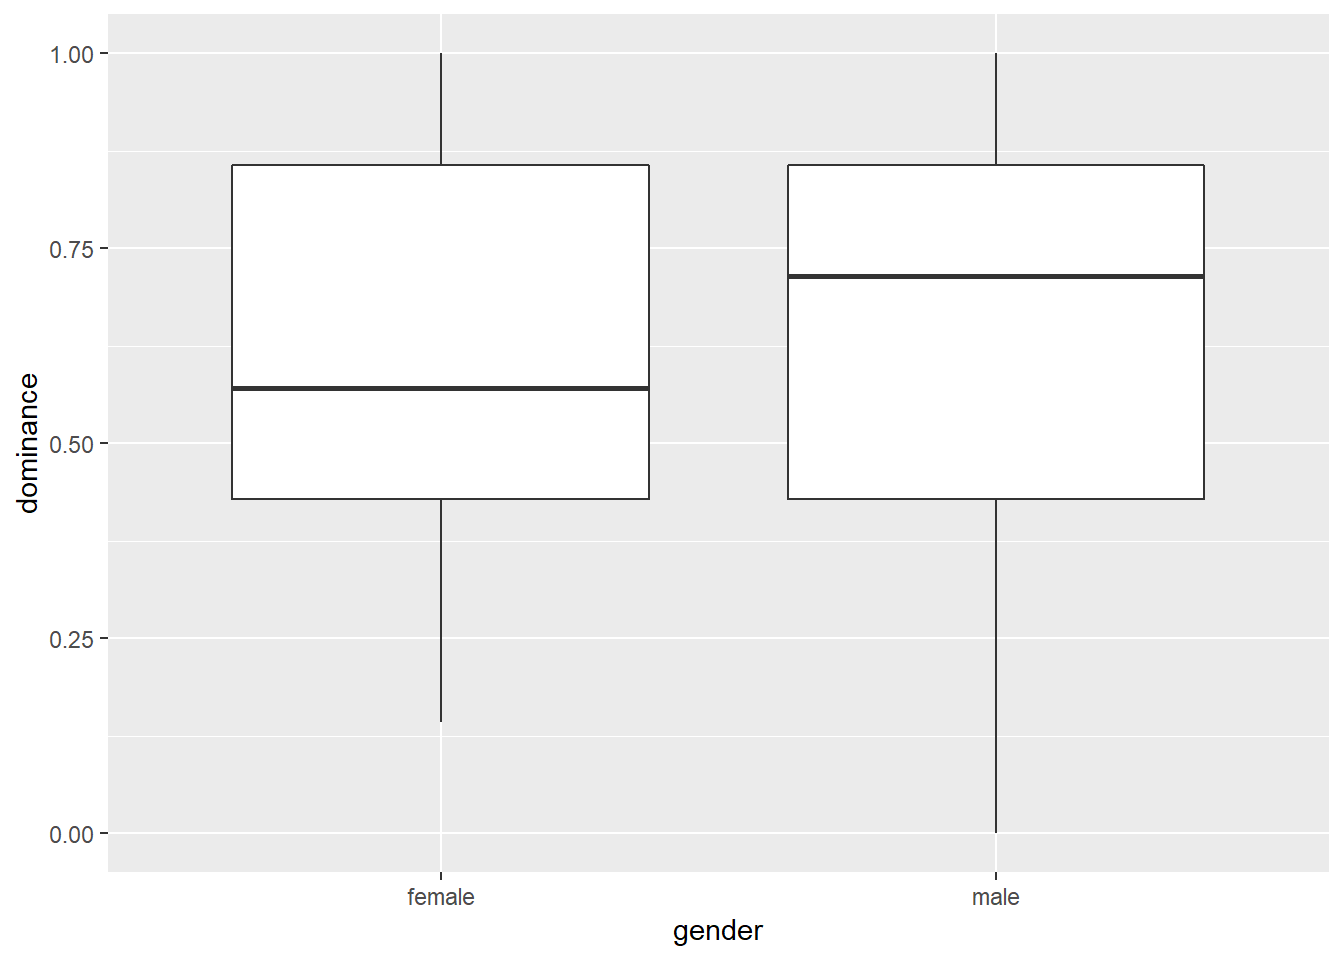
\includegraphics[width=12cm,height=8cm]{bda_independent_ttest_boxplot-1.png}
\end{center}

\begin{lstlisting}[language=R]
powercc %>% 
  group_by(gender) %>% 
  summarize(mean_dominance = mean(dominance),
            sd_dominance = sd(dominance))
            
## # A tibble: 2 x 3
##   gender mean_dominance sd_dominance
##   <chr>           <dbl>        <dbl>
## 1 female          0.614        0.247
## 2 male            0.646        0.296
\end{lstlisting}

Os homens pontuam um pouco mais alto que as mulheres, mas queremos saber se essa diferença é significativa. Um teste $t$ de amostras independentes pode fornecer a resposta (os homens e as mulheres em nosso experimento são amostras independentes), mas precisamos verificar primeiro uma suposição: as variações das duas amostras independentes são iguais?

\begin{lstlisting}[language=R]
install.packages("car") # para o teste de variancias iguais, precisamos de um pacote chamado car
library(car)

# Teste Levene para igualdade de variancias.
# Baixo valor-p indica que as variancias nao sejam iguais.
# Primeiro argumento = variavel dependente continua, segundo argumento = variavel independente categorica

leveneTest(powercc$dominance, powercc$gender) 

## Levene's Test for Homogeneity of Variance (center = median)
##        Df F value Pr(>F)
## group   1  2.1915  0.141
##       141

\end{lstlisting}

\newpage
A hipótese nula de variâncias iguais não é rejeitada (p = 0,14), para que possamos continuar com um teste t que assume variâncias iguais:

\begin{lstlisting}[language=R]
# Teste se os meios de dominancia diferem entre os sexos.
# Indique se o teste deve assumir variacoes iguais ou nao (define var.equal = FALSE para um teste que nao assume variacoes iguais).

t.test(powercc$dominance ~ powercc$gender, var.equal = TRUE) 

## 
##  Two Sample t-test
## 
## data:  powercc$dominance by powercc$gender
## t = -0.6899, df = 141, p-value = 0.4914
## alternative hypothesis: true difference in means is not equal to 0
## 95 percent confidence interval:
##  -0.12179092  0.05877722
## sample estimates:
## mean in group female   mean in group male 
##            0.6142857            0.6457926

\end{lstlisting}


Você pode relatar o seguinte: “Homens (M = 0,65, DP = 0,3) e mulheres (M = 0,61, DP = 0,25) não diferiram no grau em que se classificaram como dominantes (t (141) = -0,69 , p = 0,49). "

\subsubsection{Teste t para amostras dependentes}

Digamos que queremos testar se as pessoas estão mais dispostas a gastar em itens conspícuos do que em itens discretos. Vamos verificar os meios e os desvios padrão primeiro:

\begin{lstlisting}[language=R]
powercc %>% # nao ha necessidade de agrupar! nao estamos dividindo nossa amostra em subgrupos
  summarize(mean_cc = mean(cc), sd_cc = sd(cc),
            mean_icc = mean(icc), sd_icc = sd(icc))
            
## # A tibble: 1 x 4
##   mean_cc sd_cc mean_icc sd_icc
##     <dbl> <dbl>    <dbl>  <dbl>
## 1    6.01  1.05     3.60  0.988
\end{lstlisting}

As médias são mais altas para produtos conspícuos do que para produtos discretos, mas queremos saber se essa diferença é significativa e, portanto, realizar um teste t de amostras dependentes (cada participante classifica produtos conspícuos e discretos, portanto, essas classificações são dependentes):

\begin{lstlisting}[language=R]
t.test(powercc$cc, powercc$icc, paired = TRUE) # Teste se as medias de cc e icc sao diferentes. Indique que este eh um teste t de amostras dependentes com emparelhado = TRUE.

## 
##  Paired t-test
## 
## data:  powercc$cc and powercc$icc
## t = 25.064, df = 142, p-value < 2.2e-16
## alternative hypothesis: true difference in means is not equal to 0
## 95 percent confidence interval:
##  2.214575 2.593816
## sample estimates:
## mean of the differences 
##                2.404196

\end{lstlisting}

Você pode relatar o seguinte: “As pessoas indicaram que estavam dispostas a pagar mais (t (142) = 25.064, $p <0,001$) por produtos conspícuos (M = 6,01, DP = 1,05) do que por produtos discretos (M = 3,6, DP = 0,99). ”

\newpage

\subsubsection{Teste t para amostra única}
Digamos que queremos testar se a disposição média de pagar pelos itens visíveis foi significativamente maior que 5 (o ponto médio da escala):

\begin{lstlisting}[language=R]
t.test(powercc$cc, mu = 5) # Indique a variavel cuja media queremos comparar com um valor especifico (5).

## 
##  One Sample t-test
## 
## data:  powercc$cc
## t = 11.499, df = 142, p-value < 2.2e-16
## alternative hypothesis: true mean is not equal to 5
## 95 percent confidence interval:
##  5.833886 6.180100
## sample estimates:
## mean of x 
##  6.006993
\end{lstlisting}

Na verdade, é significativamente maior que 5. Você pode relatar o seguinte: "A WTP média para produtos conspícuos (M = 6,01, DP = 1,05) estava significativamente acima de 5 (t (142) = 11,499, $p <0,001$)."

\subsection{ANOVA bivariada}

Quando você lê um artigo acadêmico que relata um experimento, a seção de resultados geralmente começa com uma discussão dos principais efeitos dos fatores experimentais e sua interação, conforme testado por uma Análise de variância ou ANOVA. Vamos nos concentrar primeiro na \fbox{WTP} para produtos que melhoram o status. (Consideramos brevemente a \fbox{WTP} para produtos com status neutro em nossa discussão sobre testes t de amostras dependentes e discutiremos mais detalhadamente na seção ANOVA de medidas repetidas.)

Vamos inspecionar algumas estatísticas descritivas primeiro. Gostaríamos de ver a \fbox{WTP} média para produtos visíveis, o desvio padrão dessa \fbox{WTP} e o número de participantes em cada célula experimental. Já aprendemos como fazer isso no capítulo introdutório (consulte as tabelas de frequência e as estatísticas descritivas):

\begin{lstlisting}[language=R]
powercc.summary <- powercc %>% # estamos atribuindo o resumo a um objeto, porque precisaremos desse resumo para fazer um grafico de barras
  group_by(audience, power) %>% # agora agrupamos por duas variaveis
  summarize(count = n(),
            mean = mean(cc),
            sd = sd(cc))

powercc.summary
## # A tibble: 4 x 5
## # Groups:   audience [?]
##   audience power count  mean    sd
##   <fct>    <fct> <int> <dbl> <dbl>
## 1 private  low      34  6.08 1.04 
## 2 private  high     31  5.63 0.893
## 3 public   low      40  6.17 1.15 
## 4 public   high     38  6.07 1.03
\end{lstlisting}

Vemos que a diferença na \fbox{WTP} entre os participantes de alta e baixa potência é maior na condição privada do que na pública.

Vamos resumir esses resultados em um gráfico de caixa:

\begin{lstlisting}[language=R]
# ao criar um grafico de caixa, o conjunto de dados que serve como entrada para o ggplot eh o conjunto de dados completo, nao o resumo com os meios
ggplot(data = powercc, mapping = aes(x = audience, y = cc, fill = power)) + 
  geom_boxplot() # argumentos sao os mesmos que para geom_bar, mas agora fornecemos a geom_boxplot
\end{lstlisting}

\begin{center}
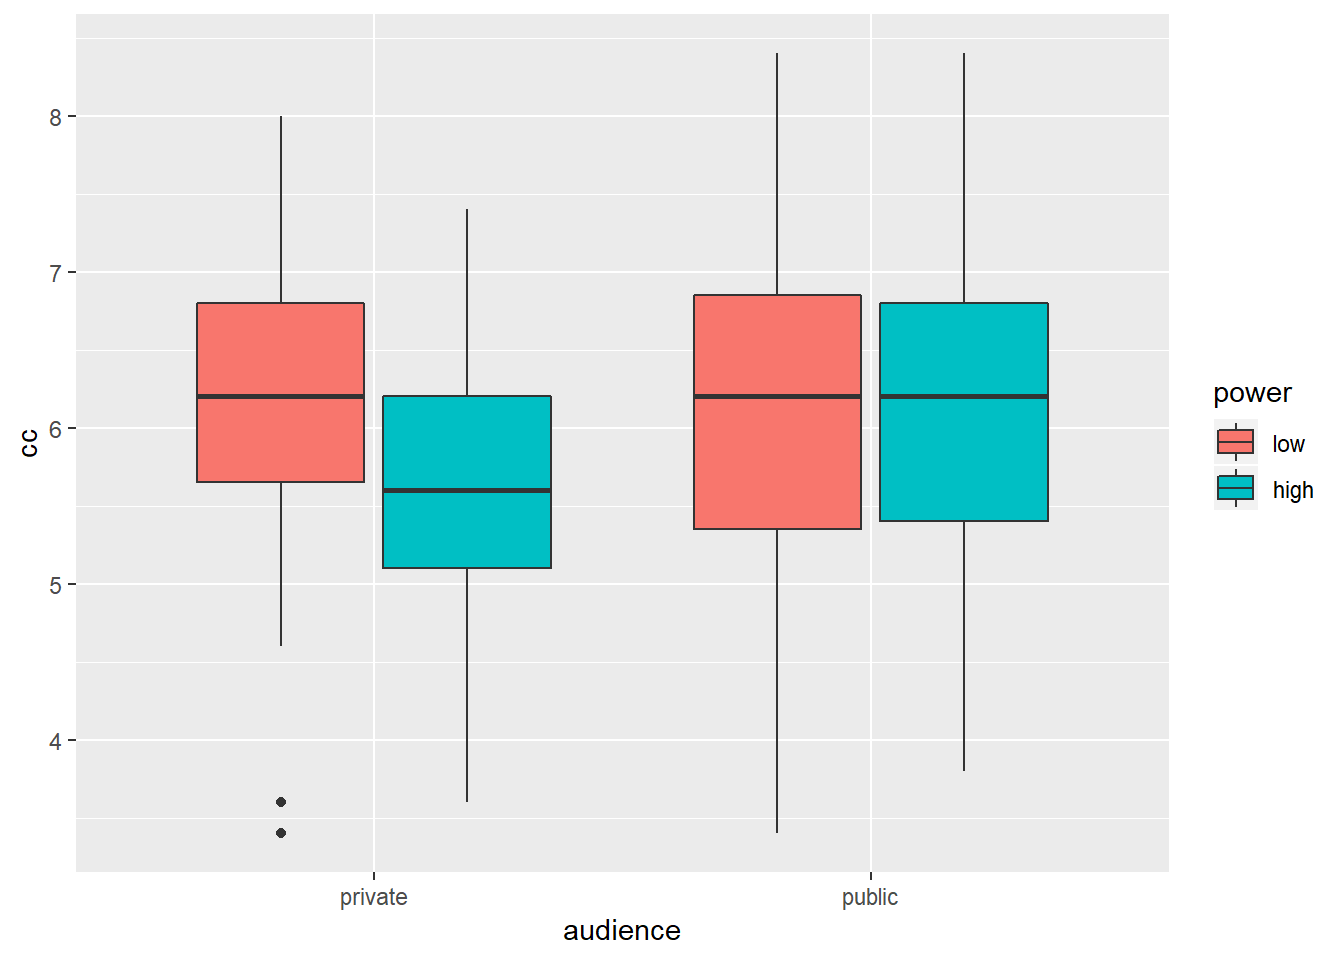
\includegraphics[width=12cm,height=8cm]{bda_boxplot-1.png}
\end{center}

Os gráficos boxplot são informativos porque nos dão uma idéia da mediana e da distribuição dos dados. No entanto, em trabalhos acadêmicos, os resultados das experiências são tradicionalmente resumidos em gráficos de barras (mesmo que os gráficos boxplots sejam mais informativos).

\begin{lstlisting}[language=R]
# ao criar um grafico de barras, o conjunto de dados que serve como entrada para o ggplot eh o resumo com os meios, nao o conjunto de dados completo
ggplot(data = powercc.summary, mapping = aes(x = audience, y = mean, fill = power)) +
  geom_bar(stat = "identity", position = "dodge")
\end{lstlisting}


\begin{center}
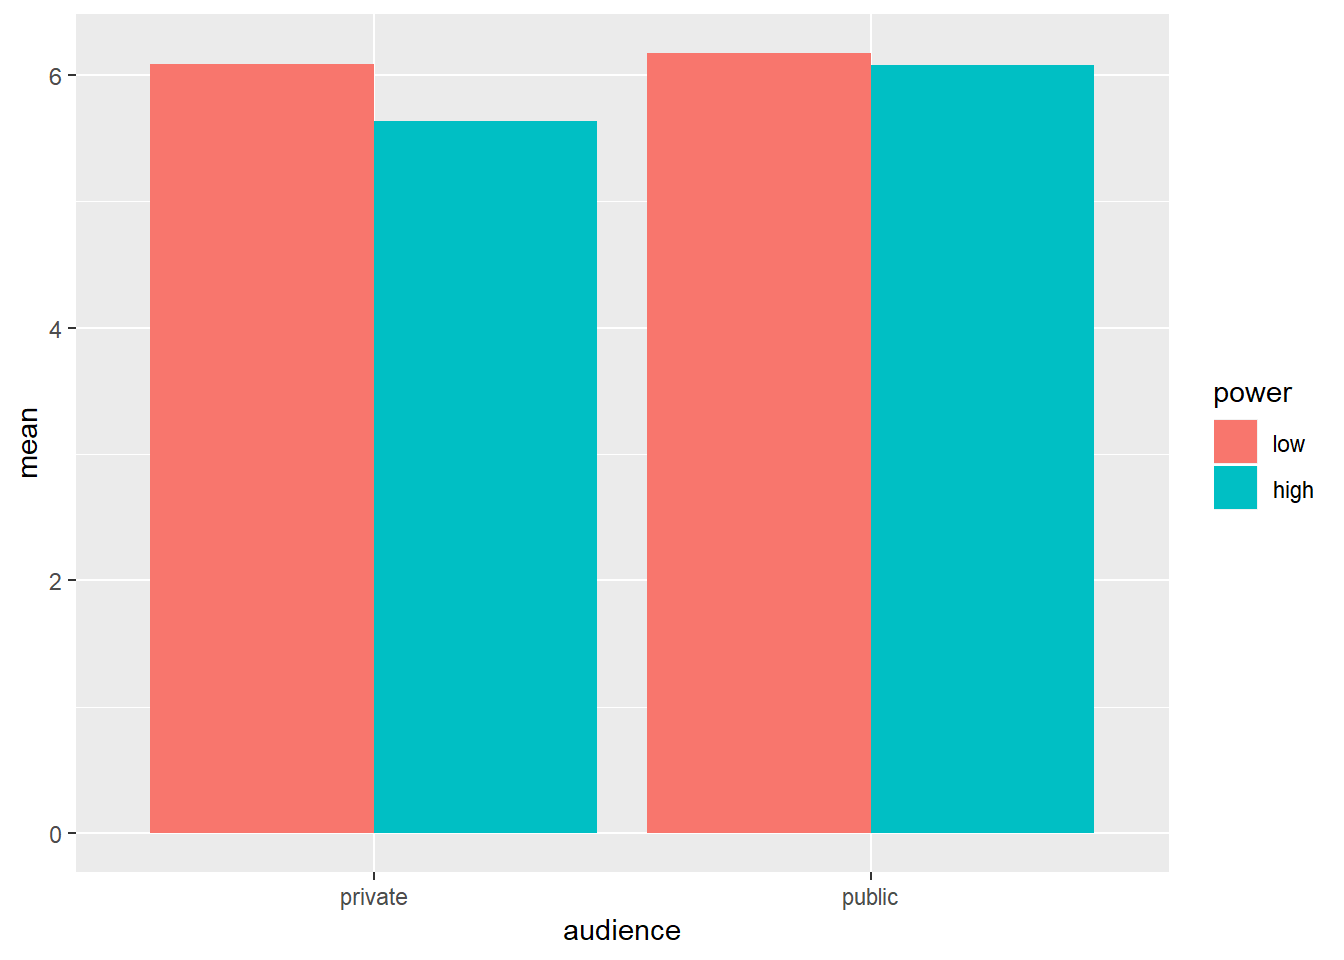
\includegraphics[width=12cm,height=8cm]{bda_barplot-1.png}
\end{center}

Para criar um gráfico de barras, informamos ao \fbox{ggplot} as variáveis que devem estar no eixo X e no eixo Y e também usamos cores diferentes para diferentes níveis de potência com o comando \fbox{fill}. Então pedimos um gráfico de barras com \fbox{geom\_bar. stat = "identity"} e \fbox{position = "dodge"} devem ser incluídos como argumentos para \fbox{geom\_bar}, mas uma discussão sobre esses argumentos está além do escopo deste tutorial.

Antes de prosseguirmos com a ANOVA, devemos verificar se suas premissas são atendidas. Discutimos as suposições da ANOVA anteriormente, mas ignoramos aqui.

Para realizar uma ANOVA, precisamos instalar alguns pacotes:

\begin{lstlisting}[language=R]
install.packages("remotes") # O pacote de controles remotos nos permite instalar pacotes armazenados no GitHub, um site para desenvolvedores de pacotes.
install.packages("car") # Tambem precisaremos do pacote do carro para executar a ANOVA (não é necessário reinstala-lo se você já tiver feito isso).

library(remotes)
install_github('samuelfranssens/type3anova') # Instale o pacote type3anova. Esta e as etapas anteriores precisam ser executadas apenas uma vez.

library(type3anova) # Carrega o pacote type3anova 
\end{lstlisting}

Agora podemos prosseguir com a ANOVA real:

\begin{lstlisting}[language=R]
# Cria um modelo linear primeiramente
# A funcao lm() toma os dados e os argumentos
# A formula tem a seguinte sintaxe: variavel dependente  ~ variavel independente
linearmodel <- lm(cc ~ power*audience, data=powercc) 
# power*audience: interacao eh calculada
# power+audience: interacao nao eh incluida

type3anova(linearmodel) # Em seguida, peça a saída no formato ANOVA. Isso fornece a soma dos quadrados do Tipo III. Observe que isso é diferente da anova (modelo linear), que fornece a soma dos quadrados do tipo I.

## # A tibble: 5 x 6
##   term                ss   df1   df2       f     pvalue
##   <chr>            <dbl> <dbl> <int>   <dbl>      <dbl>
## 1 (Intercept)    5080.       1   139 4710.    4.21e-109
## 2 power             2.64     1   139    2.45  1.20e-  1
## 3 audience          2.48     1   139    2.30  1.32e-  1
## 4 power:audience    1.11     1   139    1.03  3.13e-  1
## 5 Residuals       150.     139   139   NA    NA
\end{lstlisting}

Você pode relatar esses resultados da seguinte forma: “Nem o principal efeito do poder (F (1, 139) = 2,45, p = 0,12), nem o principal efeito do público (F (1, 139) = 2,3, p = 0,13), nem a interação entre poder e público (F (1, 139) = 1,03, p = 0,31) foi significativa. ”

\subsubsection{Seguindo com contrastes}

Ao realizar um experimento 2 x 2, geralmente fazemos a hipótese de uma interação. Uma interação significa que o efeito de uma variável independente é diferente dependendo dos níveis da outra variável independente. Na seção anterior, a ANOVA nos disse que a interação entre poder e público não era significativa. Isso significa que o efeito de alta versus baixa potência foi o mesmo na condição privada e pública e que o efeito de público versus privado foi o mesmo na condição de alta e baixa potência. Normalmente, a análise para com a não significância da interação. No entanto, faremos os testes de acompanhamento que um faria se a interação fosse significativa.

Vamos considerar o significado da célula novamente:

\begin{lstlisting}[language=R]
powercc.summary <- powercc %>% 
  group_by(audience, power) %>% 
  summarize(count = n(),
            mean = mean(cc),
            sd = sd(cc))

# ao criar um grafico de barras, o conjunto de dados que serve como entrada para o ggplot eh o resumo com os meios, nao o conjunto de dados completo
ggplot(data = powercc.summary,mapping = aes(x = audience, y = mean, fill = power)) + 
  geom_bar(stat = "identity", position = "dodge")
\end{lstlisting}

\begin{center}
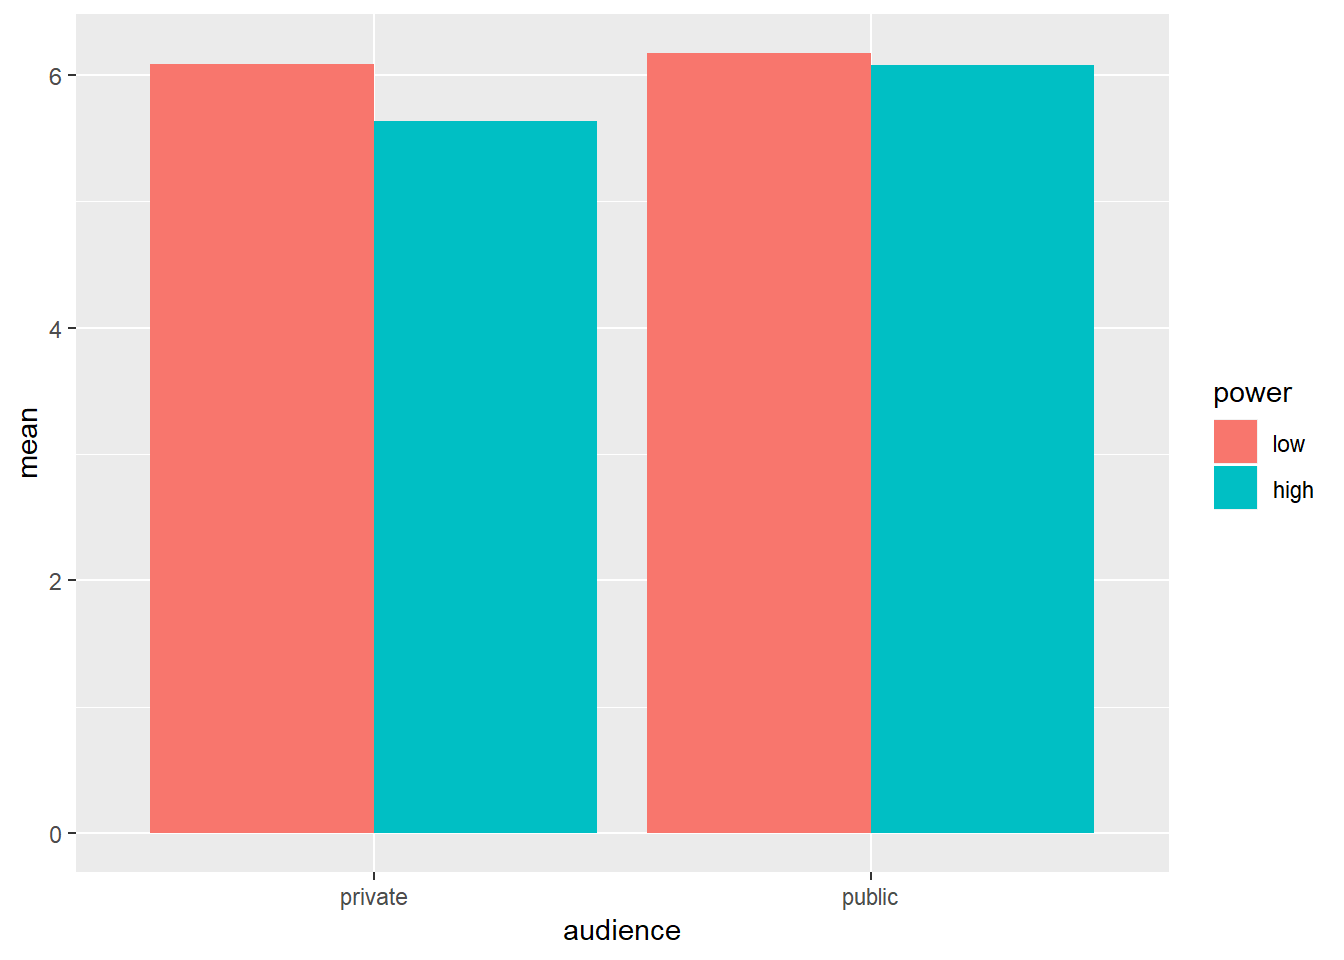
\includegraphics[width=12cm,height=8cm]{bda_contrasts0-1.png}
\end{center}


\begin{lstlisting}[language=R]
powercc.summary

## # A tibble: 4 x 5
## # Groups:   audience [2]
##   audience power count  mean    sd
##   <fct>    <fct> <int> <dbl> <dbl>
## 1 private  low      34  6.08 1.04 
## 2 private  high     31  5.63 0.893
## 3 public   low      40  6.17 1.15 
## 4 public   high     38  6.07 1.03
\end{lstlisting}

Queremos testar se a diferença entre alta e baixa potência na condição privada é significativa (baixa: 6,08 vs. alta: 5,63) e se a diferença entre alta e baixa potência na condição pública é significativa (baixa: 6,17 vs. alta : 6,07). Para fazer isso, podemos usar a função de contraste da biblioteca type3anova que instalamos anteriormente. A função de contraste usa dois argumentos: um modelo linear e uma especificação de contraste. O modelo linear é o mesmo de antes:

\begin{lstlisting}[language]
linearmodel <- lm(cc ~ power*audience, data=powercc)
\end{lstlisting}

Mas, para saber como devemos especificar nosso contraste, precisamos dar uma olhada nos coeficientes de regressão em nosso modelo linear:

\begin{lstlisting}[language=R]
summary(linearmodel)

## 
## Call:
## lm(formula = cc ~ power * audience, data = powercc)
## 
## Residuals:
##     Min      1Q  Median      3Q     Max 
## -2.7700 -0.6737  0.1177  0.7177  2.3263 
## 
## Coefficients:
##                          Estimate Std. Error t value Pr(>|t|)    
## (Intercept)               6.08235    0.17812  34.148   <2e-16 ***
## powerhigh                -0.45009    0.25792  -1.745   0.0832 .  
## audiencepublic            0.08765    0.24226   0.362   0.7181    
## powerhigh:audiencepublic  0.35378    0.34910   1.013   0.3126    
## ---
## Signif. codes:  0 '***' 0.001 '**' 0.01 '*' 0.05 '.' 0.1 ' ' 1
## 
## Residual standard error: 1.039 on 139 degrees of freedom
## Multiple R-squared:  0.03711,    Adjusted R-squared:  0.01633 
## F-statistic: 1.786 on 3 and 139 DF,  p-value: 0.1527

\end{lstlisting}

\newpage

Temos 4 coeficientes de regressão:

\begin{itemize}
    \item $\beta_{0}$ ou intercepto
    \item $\beta_{1}$ ou o coeficiente de \fbox{“powerhigh”} ou o alto nível do fator de potência (-0,45)
    \item $\beta_{2}$ ou o coeficiente para \fbox{"audiencepublic"} ou o nível público do fator público (0,09)
    \item $\beta_{3}$ ou coeficiente para: \fbox{“powerhigh:audiencepublic”} (0.35)
\end{itemize}


Vemos que a estimativa para a interceptação corresponde à média observada na célula privada de baixa potência. Adicione a isso a estimativa de \fbox{“powerhigh”} e obteremos a média observada na célula privada de alta potência. Adicione à estimativa para a interceptação, a estimativa de \fbox{"audiencepublic"} e obtenha a média observada na célula pública de baixa potência. Adicione à estimativa para a interceptação, a estimativa de \fbox{“powerhigh”}, \fbox{“audiencepublic”} e \fbox{“powerhigh:audiencepublic”} e obteremos a média observada na célula pública de alto poder. Geralmente visualizo isso em uma tabela (e salvo no meu script) para facilitar a especificação do contraste que quero testar:

\begin{lstlisting}[language=R]
#                   private             public
# low power         b0                  b0+b2
# high power        b0+b1               b0+b1+b2+b3
\end{lstlisting}

Digamos que estamos contrastando energia alta versus baixa na condição privada e testamos se ($\beta_{0}+\beta_{1}$ e $\beta_{0}$ diferem significativamente ou se ($\beta_{0}+\beta_{1})-\beta_{0}=\beta_{1}$ é significativamente diferente de zero. Nós especificamos isso da seguinte maneira:

\begin{lstlisting}[language=R]
contrast_specification <- c(0, 1, 0, 0) 

# os quatro numeros correspondentes a b0, b1, b2, b3. 
# queremos testar se b1 eh significativo, entao colocamos 1 em 2º lugar (o 1º lugar é para b0)

contrast(linearmodel, contrast_specification)

## 
##   Simultaneous Tests for General Linear Hypotheses
## 
## Fit: aov(formula = linearmodel)
## 
## Linear Hypotheses:
##        Estimate Std. Error t value Pr(>|t|)  
## 1 == 0  -0.4501     0.2579  -1.745   0.0832 .
## ---
## Signif. codes:  0 '***' 0.001 '**' 0.01 '*' 0.05 '.' 0.1 ' ' 1
## (Adjusted p values reported -- single-step method)
\end{lstlisting}

A saída nos diz que a estimativa do contraste é -0,45, que é realmente a diferença entre as médias observadas na condição privada (alta potência: 5,63 vs. baixa potência: 6,08). Você pode relatar esse resultado da seguinte forma: “O efeito de alta (M = 5,63, DP = 0,89) vs. baixa potência (M = 6,08, DP = 1,04) na condição privada foi marginalmente significativo (t (139) = -1,745 , p = 0,083). " Para obter os graus de liberdade, faça um contraste (\fbox{linearmodel}, \fbox{contrast\_specification)\$df}

Digamos que queremos testar um contraste mais complicado, ou seja, se a média na célula privada de alta potência é diferente da média das médias nas outras células. Estamos testando:

\begin{center}
$(\beta_0 + \beta_1)-1/3*[(\beta_0)+(\beta_0 +\beta_2)+(\beta_0+\beta_1+\beta_2+\beta_3)]$

\vspace{.25cm}

$=\beta_1-1/3*(\beta_1+2\beta_2+\beta_3)$

\vspace{.25cm}

$=2/3 * \beta_1-2/3 * \beta_2-1/3 * \beta_3$
\end{center}

\newpage
A especificação de contraste é a seguinte:

\begin{lstlisting}[language=R]
contrast_specification <- c(0, 2/3, -2/3, -1/3) 
contrast(linearmodel, contrast_specification)

## 
##   Simultaneous Tests for General Linear Hypotheses
## 
## Fit: aov(formula = linearmodel)
## 
## Linear Hypotheses:
##        Estimate Std. Error t value Pr(>|t|)  
## 1 == 0  -0.4764     0.2109  -2.259   0.0254 *
## ---
## Signif. codes:  0 '***' 0.001 '**' 0.01 '*' 0.05 '.' 0.1 ' ' 1
## (Adjusted p values reported -- single-step method)
\end{lstlisting}

Verifique se a estimativa realmente corresponde à diferença entre a média de alta potência, privada e a média das médias nas outras células. Você pode relatar o seguinte: “A célula privada de alta potência tinha uma WTP significativamente menor do que as outras células experimentais em nosso projeto (est = -0,476, t (139) = -2,259, p = 0,025)”.


\subsection{Análise de moderação: interação entre variáveis independentes contínuas e categóricas}

Digamos que queremos testar se os resultados do experimento dependem do nível de domínio das pessoas. Em outras palavras, os efeitos do poder e da audiência são diferentes para participantes dominantes versus participantes não dominantes? Ainda em outras palavras, existe uma interação de três vias entre poder, audiência e domínio?

Vamos criar um gráfico primeiro:

\begin{lstlisting}[language=R]
# Nossa variavel dependente eh o consumo conspicuo, nossa variavel independente (no eixo X) eh a dominancia.
# Entao, estamos tracando a relacao entre dominancia e consumo conspicuo.
# O argumento da cor diz a R que queremos um relacionamento para cada nivel de poder.

ggplot(data = powercc, mapping = aes(x = dominance, y = cc, color = power)) + 
  facet_wrap(~ audience) + # Diga a R que tambem queremos dividir por audiencia.
  geom_jitter() + # Use geom_jitter em vez de geom_point, caso contrario, os pontos serao desenhados um sobre o outro
  geom_smooth(method='lm', se=FALSE) # Desenhe uma linha de regressao linear atraves dos pontos.
\end{lstlisting}


\begin{center}
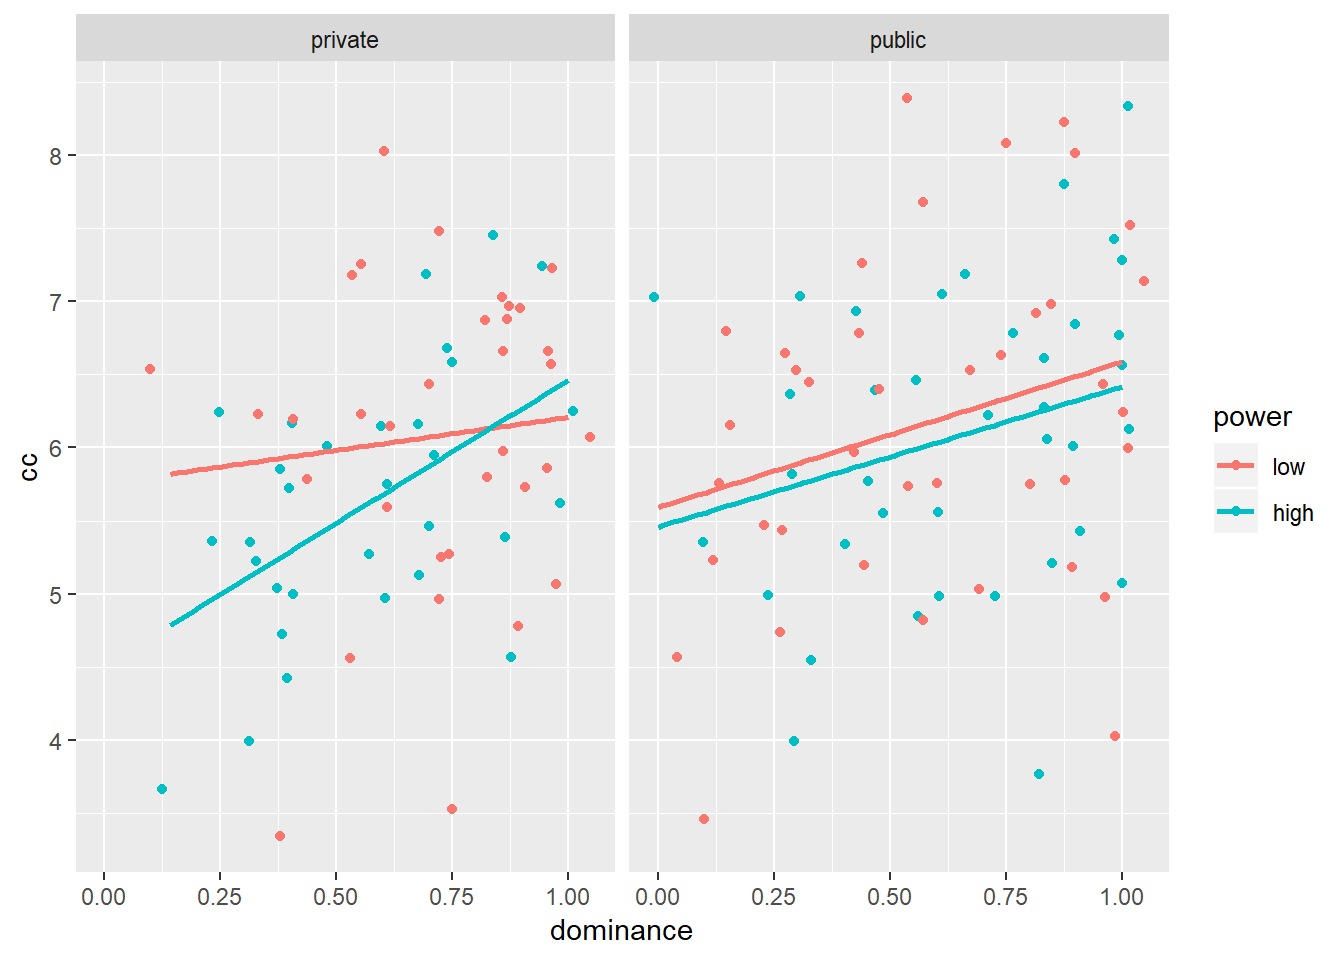
\includegraphics[width=12cm,height=8cm]{bda_interaction_graph-1.png}
\end{center}

Este gráfico é informativo. Isso nos mostra que, na condição privada, o efeito da alta versus baixa potência no consumo conspícuo é mais negativo para participantes menos dominantes do que para participantes mais dominantes. Na condição pública, o efeito da alta versus baixa potência no consumo conspícuo não difere entre os participantes menos versus os mais dominantes. Também vemos que, tanto na condição privada quanto na pública, os participantes mais vs. menos dominantes estão mais dispostos a gastar em consumo conspícuo.

Vamos verificar se a interação de três vias é significativa:

\begin{lstlisting}[language=R]
linearmodel <- lm(cc ~ power * audience * dominance, data = powercc)
type3anova(linearmodel)

## # A tibble: 9 x 6
##   term                          ss   df1   df2       f    pvalue
##   <chr>                      <dbl> <dbl> <int>   <dbl>     <dbl>
## 1 (Intercept)              525.        1   135 519.     4.35e-48
## 2 power                      2.21      1   135   2.18   1.42e- 1
## 3 audience                   0.715     1   135   0.706  4.02e- 1
## 4 dominance                 10.5       1   135  10.3    1.63e- 3
## 5 power:audience             1.44      1   135   1.42   2.35e- 1
## 6 power:dominance            1.18      1   135   1.17   2.82e- 1
## 7 audience:dominance         0.113     1   135   0.111  7.39e- 1
## 8 power:audience:dominance   1.30      1   135   1.29   2.58e- 1
## 9 Residuals                137.      135   135  NA     NA

\end{lstlisting}

Somente o efeito da dominância é significativa. Se a interação de três vias fosse significativa, poderíamos acompanhar com mais testes. Por exemplo, poderíamos testar se a interação bidirecional entre dominância e poder é significativa na condição privada, como sugere o gráfico. Para fazer isso, vamos primeiro examinar os coeficientes de regressão do nosso modelo linear:

\begin{lstlisting}[language=R]
summary(linearmodel)

## 
## Call:
## lm(formula = cc ~ power * audience * dominance, data = powercc)
## 
## Residuals:
##      Min       1Q   Median       3Q      Max 
## -2.58617 -0.63357  0.09751  0.68310  2.24067 
## 
## Coefficients:
##                                    Estimate Std. Error t value Pr(>|t|)
## (Intercept)                          5.7553     0.6019   9.561   <2e-16
## powerhigh                           -1.2490     0.7703  -1.621    0.107
## audiencepublic                      -0.1651     0.6918  -0.239    0.812
## dominance                            0.4526     0.7980   0.567    0.572
## powerhigh:audiencepublic             1.1162     0.9355   1.193    0.235
## powerhigh:dominance                  1.5021     1.1111   1.352    0.179
## audiencepublic:dominance             0.5434     0.9514   0.571    0.569
## powerhigh:audiencepublic:dominance  -1.5394     1.3561  -1.135    0.258
##                                       
## (Intercept)                        ***
## powerhigh                             
## audiencepublic                        
## dominance                             
## powerhigh:audiencepublic              
## powerhigh:dominance                   
## audiencepublic:dominance              
## powerhigh:audiencepublic:dominance    
## ---
## Signif. codes:  0 '***' 0.001 '**' 0.01 '*' 0.05 '.' 0.1 ' ' 1
## 
## Residual standard error: 1.006 on 135 degrees of freedom
## Multiple R-squared:  0.1225, Adjusted R-squared:  0.07703 
## F-statistic: 2.693 on 7 and 135 DF,  p-value: 0.01211
\end{lstlisting}

Temos oito termos em nosso modelo:
\begin{itemize}
    \item $\beta_0$ ou intercepto;
    \item $\beta_1$ ou o coeficiente para \fbox{“powerhigh”}
    \item $\beta_2$ ou o coeficiente para \fbox{“audiencepublic”}
      \item $\beta_3$ ou o coeficiente para \fbox{“dominance”}
        \item $\beta_4$ ou o coeficiente para \fbox{“powerhigh:audiencepublic”}
          \item $\beta_5$ ou o coeficiente para \fbox{“powerhigh:dominance”}
            \item $\beta_6$ ou o coeficiente para \fbox{“audiencepublic:dominance”}
              \item $\beta_7$ ou o coeficiente para \fbox{“powerhigh:audiencepublic:dominance”}
\end{itemize}

Resultando nessa tabela de coeficientes:

\begin{lstlisting}[language=R]
#                     private                         public
# low power          [b0] + (b3)                     [b0+b2] + (b3+b6)
# high power         [b0+b1] + (b3+b5)               [b0+b1+b2+b4] + (b3+b5+b6+b7)
\end{lstlisting}

Como conseguimos essa tabela? Com o modelo linear especificado acima, cada valor estimado de consumo conspícuo (a variável dependente) é uma função da condição experimental do participante e do nível de dominância do participante. Digamos que tenhamos um participante na condição pública de baixa potência com um nível de dominância de 0,5. O valor estimado do consumo conspícuo para esse participante é:


\begin{itemize}
    \item $\beta_0$ ou intercepto x 1;
    \item $\beta_1$ \fbox{“powerhigh”} (porque o participante não está na condição de alta potência)
    \item $\beta_2$ \fbox{“audiencepublic”} × 1 (na condição pública)
      \item $\beta_3$ \fbox{“dominance”} ×  0.5 (dominance = 0.5)
        \item $\beta_4$ \fbox{“powerhigh:audiencepublic”} × 0 (não no poder superior e na condição pública)
          \item $\beta_5$ \fbox{“powerhigh:dominance”} × 0 (não na condição de alta potência)
            \item $\beta_6$ \fbox{“audiencepublic:dominance”} × 1 x 0,5 (na condição pública e dominância = 0,5)
              \item $\beta_7$ \fbox{“powerhigh:audiencepublic:dominance”} × 0 (não no poder superior e na condição pública)
\end{itemize}

ou

\begin{center}
$$\beta_0 \times 1 + \beta_1 \times 0 + \beta_2 \times 1 + \beta_3 \times 0.5 + \beta_4 \times 0 + \beta_5 \times 0 + \beta_6 \times 0.5 + \beta_7 \times 0$

$= [\beta_0 + \beta_2] + (\beta_3 + \beta_6) \times 0.5$

\vspace{.25cm}

$= [5.76 + -0.17] + (0.45 + 0.54) * 0.5 = 6.09$
\end{center}


Verifique o gráfico para ver se isso realmente corresponde ao consumo conspícuo estimado de um participante com dominância = 0,5 na célula pública de baixa potência.

A fórmula geral para a célula pública de baixa potência é a seguinte:

$$
[\beta_0 + \beta_2] + (\beta_3 + \beta_6)\times\mbox{dominance}
$$

e podemos obter as fórmulas para as diferentes células de maneira semelhante. Vemos que em cada célula, o coeficiente entre colchetes é o valor estimado na medida de consumo conspícuo para um participante que pontua 0 em dominância. O coeficiente entre parênteses arredondados é o aumento estimado na medida de consumo conspícuo para cada aumento de uma unidade no domínio. Em outras palavras, os coeficientes entre colchetes representam a interceptação e os coeficientes entre colchetes representam a inclinação da linha que representa a regressão do consumo conspícuo (Y) na dominância (X) dentro de cada célula experimental (ou seja, cada potência e público-alvo) combinação).

Um teste da interação entre poder e dominância dentro da condição privada se resumiria a testar se as linhas azul e vermelha no painel esquerdo da figura acima devem ser consideradas paralelas ou não. Se eles são paralelos, o efeito da dominância no consumo conspícuo é o mesmo nas condições de baixa e alta potência. Se eles não são paralelos, o efeito da dominância é diferente nas condições de baixa e alta potência. Em outras palavras, devemos testar se os coeficientes de regressão são iguais dentro de baixa potência, privado e dentro de alta potência, privado. Em outras palavras, testamos se $(\beta_3+\beta_5)-\beta_3=\beta_5$ é igual a zero:

\begin{lstlisting}[language=R]
# agora temos oito numeros correspondentes aos oito coeficientes de regressao
# queremos testar se b5 eh significativo, entao colocamos 1 em 6º lugar (o 1º lugar é para b0)

contrast_specification <- c(0, 0, 0, 0, 0, 1, 0, 0)

contrast(linearmodel, contrast_specification)

## 
##   Simultaneous Tests for General Linear Hypotheses
## 
## Fit: aov(formula = linearmodel)
## 
## Linear Hypotheses:
##        Estimate Std. Error t value Pr(>|t|)
## 1 == 0    1.502      1.111   1.352    0.179
## (Adjusted p values reported -- single-step method)

\end{lstlisting}

A interação não é significativa, no entanto. Você pode relatar o seguinte: “Dentro da condição privada, não houve interação entre poder e dominância (t (135) = 1,352, p = 0,18).”

\vspace{.25cm}
\subsubsubsection{\textbf{Análise spotlight}}
\vspace{.25cm}


Em breve.

\subsection{ANCOVA}

Descobrimos que nossas condições experimentais não afetam significativamente o consumo conspícuo:

\begin{lstlisting}[language=R]
linearmodel1 <- lm(cc ~ power*audience, data = powercc)
type3anova(linearmodel1)

## # A tibble: 5 x 6
##   term                ss   df1   df2       f     pvalue
##   <chr>            <dbl> <dbl> <int>   <dbl>      <dbl>
## 1 (Intercept)    5080.       1   139 4710.    4.21e-109
## 2 power             2.64     1   139    2.45  1.20e-  1
## 3 audience          2.48     1   139    2.30  1.32e-  1
## 4 power:audience    1.11     1   139    1.03  3.13e-  1
## 5 Residuals       150.     139   139   NA    NA

\end{lstlisting}

Por um lado, isso pode significar que simplesmente não há efeitos das condições experimentais no consumo conspícuo. Por outro lado, isso poderia significar que as manipulações experimentais não são fortes o suficiente ou que há muita variação inexplicada em nossa variável dependente (ou ambas). Podemos reduzir a variação inexplicável em nossa variável dependente, no entanto, incluindo uma variável em nosso modelo que suspeitamos estar relacionada à variável dependente. No nosso caso, suspeitamos que a disposição de gastar em consumo discreto (\fbox{icc}) esteja relacionada à disposição de gastar em consumo conspícuo. Embora \fbox{icc} seja uma variável contínua, podemos incluí-la como uma variável independente em nossa ANOVA e isso nos permitirá reduzir a variação inexplicável em nossa variável dependente:

\begin{lstlisting}[language=R]
linearmodel2 <- lm(cc ~ power*audience + icc, data = powercc)
type3anova(linearmodel2)

## # A tibble: 6 x 6
##   term               ss   df1   df2      f    pvalue
##   <chr>           <dbl> <dbl> <int>  <dbl>     <dbl>
## 1 (Intercept)    209.       1   138 221.    1.85e-30
## 2 power            1.88     1   138   1.99  1.60e- 1
## 3 audience         1.14     1   138   1.21  2.74e- 1
## 4 icc             19.6      1   138  20.8   1.13e- 5
## 5 power:audience   1.96     1   138   2.08  1.52e- 1
## 6 Residuals      130.     138   138  NA    NA

\end{lstlisting}

Vemos que \fbox{icc} está relacionado à variável dependente e, portanto, que a soma dos quadrados dos resíduos desse modelo, ou seja, a variação inexplicada em nossa variável dependente, é menor (130,32) do que a do modelo sem icc (149,93). Os valores p dos fatores experimentais não diminuem, no entanto. Você pode relatar o seguinte: “Controlando a disposição de gastar em consumo discreto, nem o principal efeito do poder (F (1, 138) = 1,99, p = 0,16), nem o principal efeito do público (F (1, 138 ) = 1,21, p = 0,27), nem a interação entre poder e público (F (1, 138) = 2,08, p = 0,15) foi significativa. ”

Chamamos essa análise de ANCOVA porque icc é uma covariável (abrange ou está relacionada à nossa variável dependente).


\subsection{Medidas repetidas ANOVA}

Neste experimento, temos mais de uma medida por unidade de observação, ou seja, disposição para gastar em produtos conspícuos e disposição para gastar em produtos discretos. Uma ANOVA de medidas repetidas pode ser usada para testar se os efeitos das condições experimentais são diferentes para produtos conspícuos versus inconspícuos.

Para executar uma ANOVA de medidas repetidas, precisamos reestruturar nosso quadro de dados de amplo a longo. Um amplo quadro de dados possui uma linha por unidade de observação (em nosso experimento: uma linha por participante) e uma coluna por observação (em nosso experimento: uma coluna para os produtos conspícuos e uma coluna para os produtos inconspícuos). Um quadro de dados longo possui uma linha por observação (em nosso experimento: duas linhas por participante, uma linha para o produto conspícuo e uma linha para o produto inconspícuo) e uma coluna extra que indica com que tipo de observação estamos lidando (conspícua ou imperceptível). Vamos converter o quadro de dados e ver como os quadros de dados amplos e longos diferem um do outro.

\begin{lstlisting}[language=R]
powercc.long <- powercc %>% 
  gather(consumption_type, wtp, cc, icc)

# Converter de grande para longo significa que estamos empilhando varias colunas umas sobre as outras. Para isso, precisamos de uma variavel extra para acompanhar qual coluna estamos lidando.
# A funcao de coleta converte conjuntos de dados de amplos para longos.
# O primeiro argumento (consumer_type) nos dira com qual coluna estamos lidando. Essa eh a variavel que armazenara os nomes das colunas que estamos empilhando.
# O segundo argumento (wtp) armazenara as colunas reais empilhadas umas sobre as outras.
# Os argumentos a seguir sao as colunas que queremos empilhar.

# Entao, dizemos ao gather para criar duas novas variaveis: tipo_de_consumo e vontade de pagar, para representar o empilhamento de um determinado numero de colunas.

# Vamos dizer ao R para nos mostrar apenas as colunas relevantes (isto eh apenas para fins de apresentacao):

powercc.long %>%
  select(subject, power, audience, consumption_type, wtp) %>% 
  arrange(subject)
  
## # A tibble: 286 x 5
##    subject power audience consumption_type   wtp
##    <fct>   <fct> <fct>    <chr>            <dbl>
##  1 1       high  public   cc                 5  
##  2 1       high  public   icc                2.6
##  3 2       low   public   cc                 7.6
##  4 2       low   public   icc                4  
##  5 3       low   public   cc                 5.4
##  6 3       low   public   icc                3.4
##  7 4       low   public   cc                 8.4
##  8 4       low   public   icc                5.2
##  9 5       high  public   cc                 7.8
## 10 5       high  public   icc                3  
## # ... with 276 more rows

\end{lstlisting}

Temos duas linhas por assunto, uma coluna de disposição para pagar e outra coluna (tipo de consumo) que indica se está disposta a pagar por produtos visíveis ou imperceptíveis. Compare isso com o amplo conjunto de dados:

\begin{lstlisting}[language=R]
powercc %>% 
  select(subject, power, audience, cc, icc) %>% 
  arrange(subject) # Mostre somente as colunas relevantes
  
## # A tibble: 143 x 5
##    subject power audience    cc   icc
##    <fct>   <fct> <fct>    <dbl> <dbl>
##  1 1       high  public     5     2.6
##  2 2       low   public     7.6   4  
##  3 3       low   public     5.4   3.4
##  4 4       low   public     8.4   5.2
##  5 5       high  public     7.8   3  
##  6 6       high  public     7.2   5  
##  7 7       low   public     4.8   4  
##  8 8       high  public     6.6   4.4
##  9 9       low   public     5.8   4.2
## 10 10      high  public     6.8   3.4
## # ... with 133 more rows

\end{lstlisting}


Temos uma linha por assunto e duas colunas, uma para cada tipo de produto.

Agora podemos realizar uma medida repetida ANOVA. Para isso, precisamos do pacote \fbox{ez}.

\begin{lstlisting}[language=R]
install.packages("ez") # Precisamos do pacote ez para RM ANOVA
library(ez)

\end{lstlisting}

Queremos testar se a interação entre poder e público é diferente para produtos conspícuos e inconspícuos. Vamos dar uma olhada em um gráfico primeiro:

\begin{lstlisting}[language=R]
powercc.long.summary <- powercc.long %>% # para um grafico de barras precisamos de summary primeiro
  group_by(power, audience, consumption_type) %>% # agrupa por tres variaveis independentes
  summarize(wtp = mean(wtp)) # obtem a media de wtp

ggplot(data = powercc.long.summary, mapping = aes(x = audience, y = wtp, fill = power)) + 
  facet_wrap(~ consumption_type) + # create a panel for each consumption type
  geom_bar(stat = "identity", position = "dodge")
\end{lstlisting}


\begin{center}
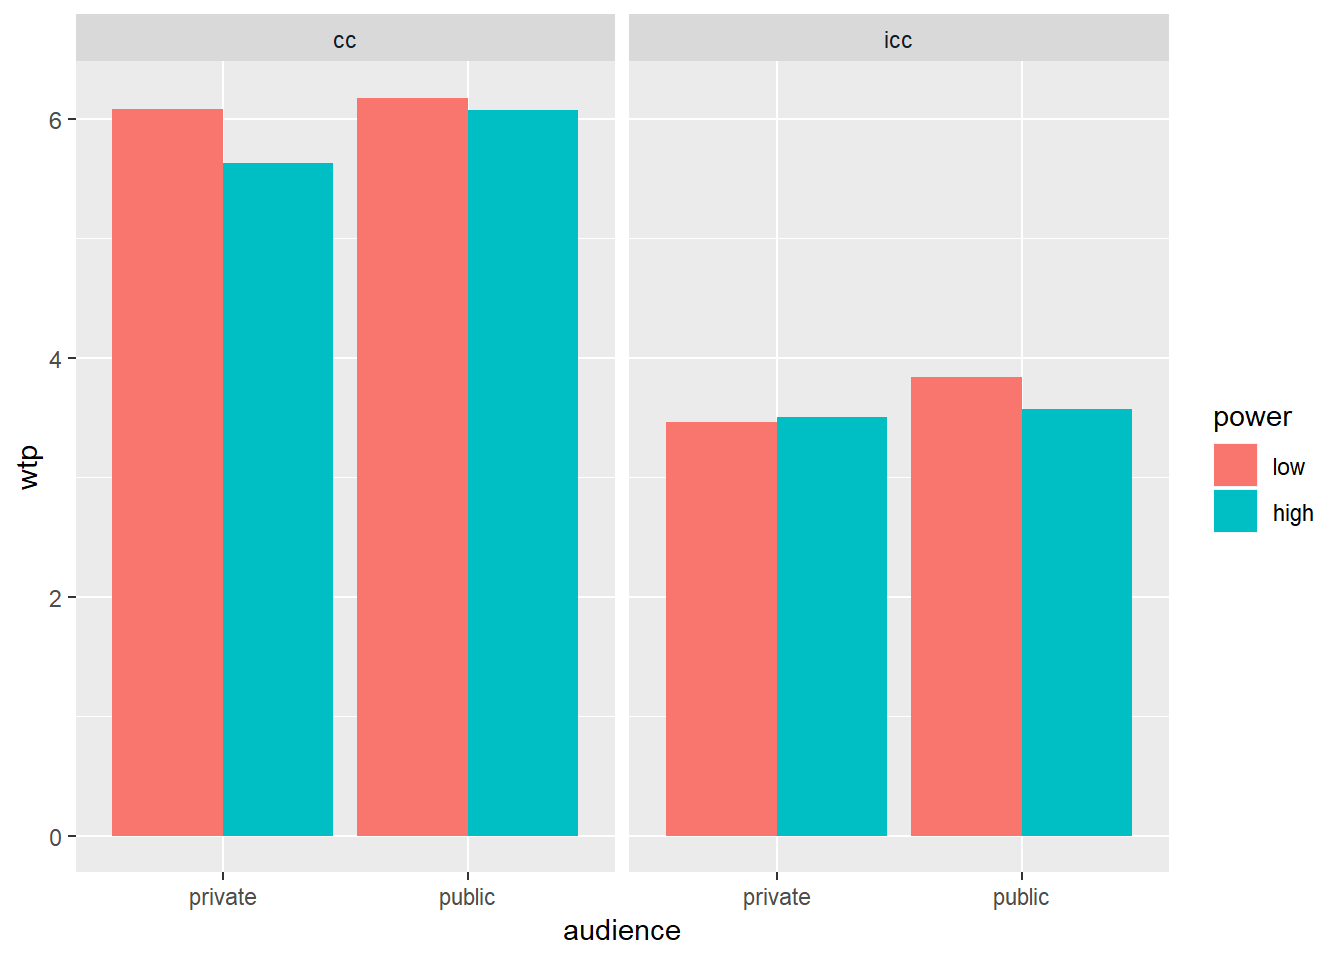
\includegraphics[width=12cm,height=8cm]{bda_rmanova_graph-1.png}
\end{center}

Agora podemos testar formalmente a interação de três vias:

\begin{lstlisting}[language=R]
# Especifique os dados, a variavel dependente, o identificador (wid),
# a variavel que representa a condicao dentro dos sujeitos e as variaveis que representam as condicoes entre os sujeitos.

ezANOVA(data = powercc.long, dv = wtp, wid = subject, within = consumption_type, between = power*audience)

## $ANOVA
##                            Effect DFn DFd            F            p p<.05
## 2                           power   1 139 1.867530e+00 1.739647e-01      
## 3                        audience   1 139 2.977018e+00 8.667716e-02      
## 5                consumption_type   1 139 6.303234e+02 1.687352e-53     *
## 4                  power:audience   1 139 5.801046e-03 9.393977e-01      
## 6          power:consumption_type   1 139 4.719313e-01 4.932445e-01      
## 7       audience:consumption_type   1 139 2.700684e-02 8.697041e-01      
## 8 power:audience:consumption_type   1 139 2.982598e+00 8.638552e-02      
##            ges
## 2 9.061619e-03
## 3 1.436772e-02
## 5 5.915501e-01
## 4 2.840440e-05
## 6 1.083172e-03
## 7 6.204919e-05
## 8 6.806406e-03

\end{lstlisting}

Vemos nesses resultados que a interação de três vias entre poder, público e tipo de consumo é marginalmente significativa. Você pode relatar o seguinte: "Uma ANOVA de medidas repetidas estabeleceu que a interação de três vias entre poder, público e tipo de consumo era marginalmente significativa (F (1, 139) = 2,98, p = 0,086).

\newpage
\section{Análise de componentes principais para mapas perceptivos (office dataset)}

Neste capítulo, você aprenderá como realizar uma análise de componentes principais e visualizar os resultados em um mapa perceptivo.

Digamos que tenhamos um conjunto de observações que diferem entre si em várias dimensões; por exemplo, temos várias marcas de uísque (observações) classificadas em vários atributos, como corpo, doçura, sabor, etc. (dimensões). Se algumas dessas dimensões estiverem fortemente correlacionadas, deve ser possível descrever as observações por um número menor (que o original) de dimensões sem perder muita informação. Por exemplo, doçura e frutificação podem ser altamente correlacionadas e, portanto, podem ser substituídas por uma variável. Essa redução de dimensionalidade é o objetivo da análise de componentes principais.

\subsection{Dados}
\subsubsection{Importação}

Analisaremos os dados de uma pesquisa na qual os entrevistados foram solicitados a classificar quatro marcas de equipamentos de escritório em seis dimensões. Faça o download dos dados \href{http://users.telenet.be/samuelfranssens/tutorial_data/perceptual_map_office.xlsx}{aqui} e importe-os para o \faRProject:


\begin{lstlisting}[language=R]
library(tidyverse)
library(readxl)

office <- read_excel("perceptual_map_office.xlsx","attributes") # nao esqueca de carregar o pacote readxl

\end{lstlisting}

\subsubsection{Manipulação}


\begin{lstlisting}[language=R]
office # visualiza os dados
\end{lstlisting}

O conjunto de dados consiste em um identificador, a marca do equipamento de escritório (\fbox{brand}) e a classificação média (entre os entrevistados) de cada marca em seis atributos: escolha grande (\fbox{large\_choice}), preços baixos (\fbox{low\_prices}), qualidade do serviço (\fbox{service\_quality}), qualidade do produto (\fbox{product\_quality}), conveniência (\fbox{convenience}) e pontuação da preferência (\fbox{preference\_score}). Vamos fatorar o identificador:


\begin{lstlisting}[language=R]
office <- office %>% 
  mutate(brand = factor(brand))
\end{lstlisting}


\subsubsection{Recapitulação: importação e manipulação}

Aqui está o que fizemos até agora, em uma sequência ordenada de operações canalizadas/pipe (faça o download dos dados aqui):

\begin{lstlisting}[language=R]
library(tidyverse)
library(readxl)

office <- read_excel("perceptual_map_office.xlsx","attributes") %>% # 
  mutate(brand = factor(brand))
\end{lstlisting}



\subsection{Quantos fatores devemos considerar ?}

O objetivo da análise de componentes principais é reduzir o número de dimensões que descrevem nossos dados, sem perder muitas informações. O primeiro passo na análise de componentes principais é decidir o número de componentes ou fatores principais que queremos manter. Para nos ajudar a decidir, usaremos a função PCA do \fbox{pacote FactoMineR}:

\begin{lstlisting}[language=R]
install.packages("FactoMineR")
library(FactoMineR)
\end{lstlisting}

\newpage

Para poder usar a \fbox{função PCA}, precisamos primeiro transformar o quadro de dados:

\begin{lstlisting}[language=R]
office.df <- office %>% 
  select(- brand) %>% # A entrada para a analise de componentes principais deve ser apenas as dimensoes, nao o (s) identificador (es); portanto, vamos remover os identificadores.
  as.data.frame() # altere o tipo do objeto para 'data.frame'. Isso eh necessario para a funcao PCA

rownames(office.df) <- office$brand # Defina os nomes das linhas do data.frame para as marcas (isso eh importante mais tarde ao fazer um biplot)
\end{lstlisting}

Agora podemos prosseguir com a análise de componentes principais:

\begin{lstlisting}[language=R]
office.pca <- PCA(office.df, graph=FALSE) # Realizar a analise de componentes principais

office.pca$eig # e veja a tabela com informacoes sobre variancia explicada

##        eigenvalue percentage of variance cumulative percentage of variance
## comp 1  4.2656310              71.093850                          71.09385
## comp 2  1.6197932              26.996554                          98.09040
## comp 3  0.1145758               1.909596                         100.00000
\end{lstlisting}


Se olharmos para esta tabela, veremos que dois componentes explicam 98,1\% da variância nas classificações. Isso já é bastante e sugere que podemos fazer com segurança duas dimensões para descrever nossos dados. Uma regra prática aqui é que a variância cumulativa explicada pelos componentes deve ser de pelo menos 70\%.

\subsection{Análise de Componentes Principais}

Vamos reter apenas dois componentes ou fatores:

\begin{lstlisting}[language=R]
office.pca.two <- PCA(office.df, ncp = 2, graph=FALSE) #Peca dois fatores preenchendo o argumento ncp.
\end{lstlisting}

\subsubsection{Cargas fatoriais}

Agora podemos inspecionar a tabela com as cargas fatoriais:

\begin{lstlisting}[language=R]
office.pca.two$var$cor %>% #tabela com cargas fatoriais varimax 
#, mas solicite uma rotacao varimax para melhorar a interpretacao

## $loadings
## 
## Loadings:
##                  Dim.1  Dim.2 
## large_choice      0.516 -0.850
## low_prices       -0.990       
## service_quality   0.912 -0.410
## product_quality   0.964       
## convenience       0.175  0.978
## preference_score  0.708 -0.706
## 
##                Dim.1 Dim.2
## SS loadings    3.538 2.347
## Proportion Var 0.590 0.391
## Cumulative Var 0.590 0.981
## 
## $rotmat
##           [,1]       [,2]
## [1,] 0.8515627 -0.5242528
## [2,] 0.5242528  0.8515627
\end{lstlisting}


Essas cargas são as correlações entre as dimensões originais  (\fbox{large\_choice}, \fbox{low\_prices}, etc.) e dois fatores são extraídos (\fbox{Dim.1 and Dim.2}). Nós vemos que \fbox{low\_prices}, \fbox{service\_quality}, e \fbox{product\_quality} pontuação alta no primeiro fator, enquanto \fbox{large\_choice}, \fbox{convenience}, e \fbox{preference\_score} pontuação alta no segundo fator. Poderíamos, portanto, dizer que o primeiro fator descreve o preço e a qualidade da marca e que o segundo fator descreve a conveniência das lojas da marca.

Também queremos saber quanto cada uma das seis dimensões é explicada pelos fatores extraídos. Para isso, precisamos calcular a comunalidade e / ou seu complemento, a singularidade das dimensões:

\begin{lstlisting}[language=R]
loadings <- as_tibble(office.pca.two$var$cor) %>% # Precisamos capturar os carregamentos como um quadro de dados em um novo objeto. Use as_tibble(), caso contrario, nao podemos acessar os diferentes fatores

  mutate(variable = rownames(office.pca.two$var$cor), # manter o controle dos nomes das linhas (eles sao removidos ao converter para tibble)
         communality = Dim.1^2 + Dim.2^2, 
         uniqueness = 1 - communality) # O operador ^ eleva um valor a uma determinada potencia. Para calcular a comunalidade, precisamos somar os quadrados das cargas em cada fator.
         
loadings
## # A tibble: 6 x 5
##    Dim.1  Dim.2 variable         communality uniqueness
##    <dbl>  <dbl> <chr>                  <dbl>      <dbl>
## 1  0.885 -0.453 large_choice           0.988   0.0116  
## 2 -0.845 -0.516 low_prices             0.980   0.0198  
## 3  0.991  0.128 service_quality        0.999   0.000669
## 4  0.841  0.473 product_quality        0.930   0.0696  
## 5 -0.364  0.925 convenience            0.988   0.0124  
## 6  0.973 -0.230 preference_score       0.999   0.000524
\end{lstlisting}

A comunalidade de uma variável é a porcentagem da variação dessa variável que é explicada pelos fatores. Seu complemento é chamado de exclusividade. A exclusividade (unicidade) pode ser puro erro de medição ou pode representar algo que é medido de forma confiável por essa variável específica, mas não por nenhuma das outras variáveis. Quanto maior a exclusividade, maior a probabilidade de que seja mais do que apenas erro de medição. Uma exclusividade superior a 0,6 é geralmente considerada alta. Se a exclusividade for alta, a variável não será bem explicada pelos fatores. Vemos que, para todas as dimensões, a comunalidade é alta e, portanto, a singularidade é baixa; portanto, todas as dimensões são bem capturadas pelos fatores extraídos.

\subsubsection{Plotando as cargas fatoriais}

Também podemos plotar as cargas. Para isso, precisamos de outro \fbox{pacote chamado factoextra}:

\begin{lstlisting}[language=R]
install.packages("factoextra")
library(factoextra)
fviz_pca_var(office.pca.two, repel = TRUE) # o argumento repel = TRUE garante que o texto seja exibido corretamente no grafico
\end{lstlisting}


\begin{center}
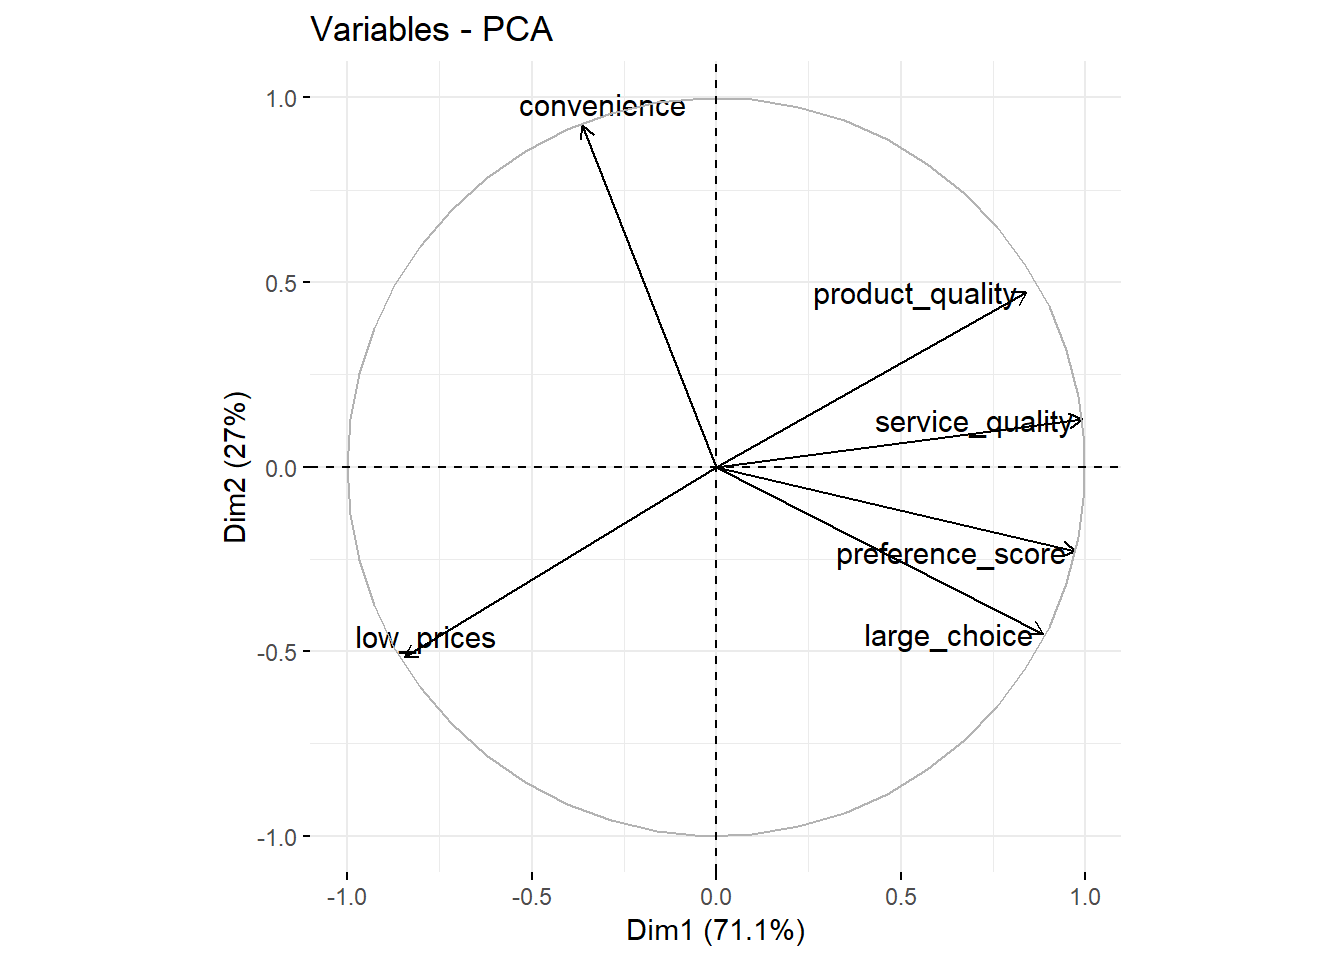
\includegraphics[width=12cm,height=8cm]{perceptual_loading_plot-1.png}
\end{center}

Nós vimos que \fbox{large\_choice}, \fbox{service\_quality}, \fbox{product\_quality} e \fbox{preference\_score} têm pontuações altas no primeiro fator (o Dim1 do eixo X) e essa conveniência tem uma pontuação alta no segundo fator (o Dim2 do eixo Y). Também podemos adicionar as observações (as diferentes marcas) a esse gráfico:

\newpage

\begin{lstlisting}[language=R]
fviz_pca_biplot(office.pca.two, repel = TRUE) # tracar as cargas e as marcas juntas em uma trama
\end{lstlisting}



\begin{center}
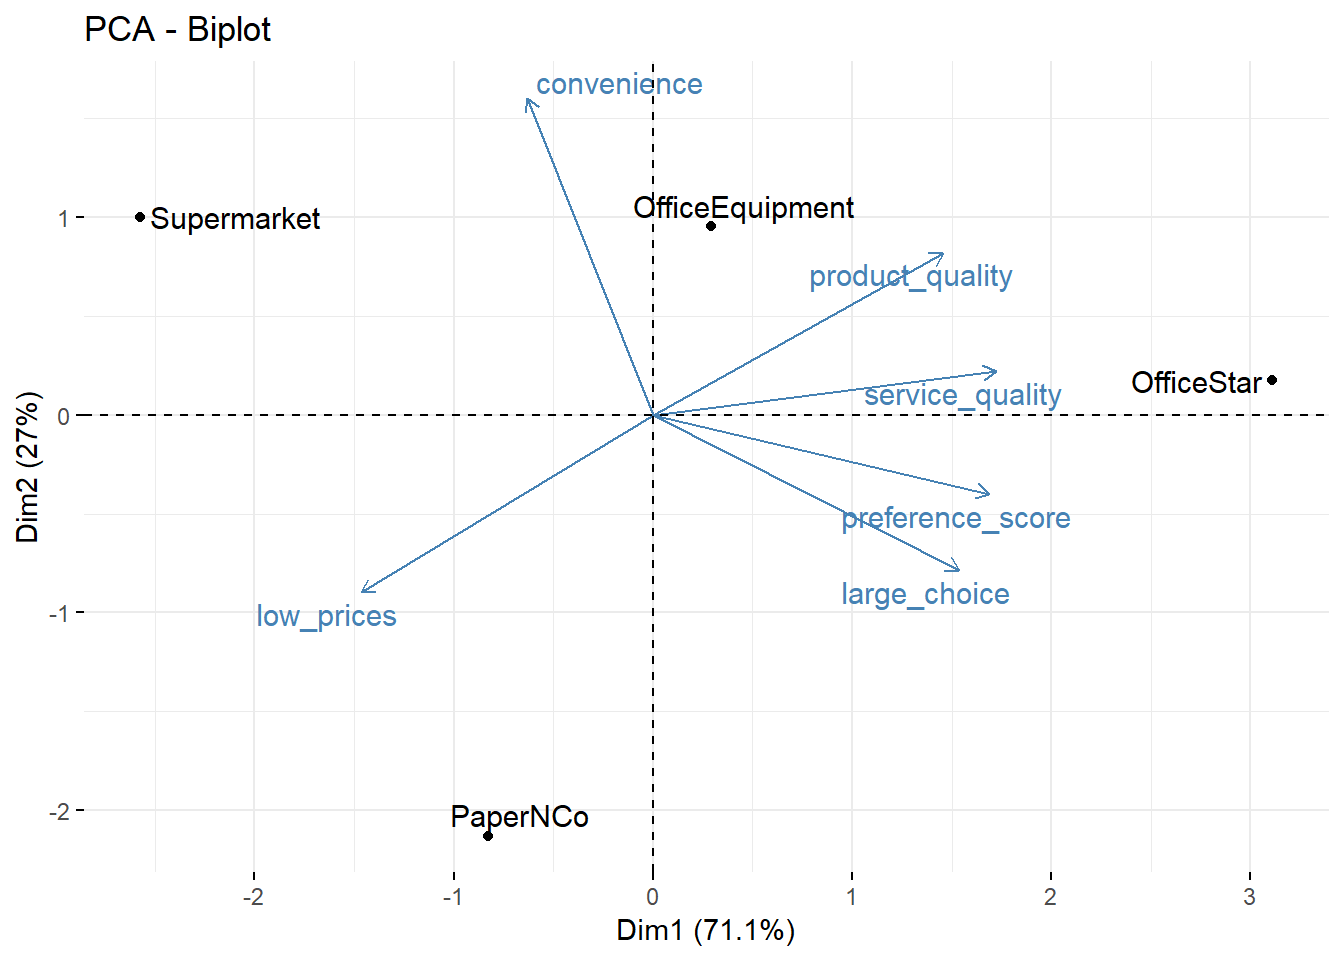
\includegraphics[width=12cm,height=8cm]{perceptual_biplot-1.png}
\end{center}

Isso também é chamado de biplot. Podemos ver, por exemplo, que o \fbox{OfficeStar} tem uma pontuação alta no primeiro fator.

\newpage
\section{Análise de componentes principais para mapas perceptivos (toothpaste dataset)}

Neste capítulo, você aprenderá como realizar uma análise de componentes principais e visualizar os resultados em um mapa perceptivo.

Digamos que tenhamos um conjunto de observações que diferem entre si em várias dimensões; por exemplo, temos várias marcas de uísque (observações) classificadas em vários atributos, como corpo, doçura, sabor, etc. (dimensões ) Se algumas dessas dimensões estiverem fortemente correlacionadas, deve ser possível descrever as observações por um número menor (que o original) de dimensões sem perder muita informação. Por exemplo, doçura e frutificação podem ser altamente correlacionadas e, portanto, podem ser substituídas por uma variável. Essa redução de dimensionalidade é o objetivo da análise de componentes principais.

\subsection{Dados}
\subsubsection{Importação}

Analisaremos os dados de uma pesquisa na qual 60 consumidores foram convidados a responder a seis perguntas sobre pasta de dente. Esses dados foram coletados pelos criadores do \fbox{Radiant}, que é um pacote do \faRProject para análise de negócios que usaremos posteriormente. Faça o download dos dados \href{http://users.telenet.be/samuelfranssens/tutorial_data/toothpaste.xlsx}{aqui} e importe-os para o \faRProject:

\begin{lstlisting}[language=R]
library(tidyverse)
library(readxl)

toothpaste <- read_excel("toothpaste.xlsx")

\end{lstlisting}

\subsubsection{Manipulação}

\begin{lstlisting}[language=R]
toothpaste # Visualiza os dados
\end{lstlisting}

O conjunto de dados consiste em um identificador, \fbox{consumer}, e as classificações do entrevistado sobre a importância de seis atributos de pasta de dente: \fbox{prevents\_cavities}, \fbox{shiny\_teeth}, \fbox{strengthens\_gums}, \fbox{freshens\_breath}, \fbox{decay\_prevention\_unimportant}, and \fbox{attractive\_teeth}. Nos também temos os respondentes \fbox{age} e \fbox{gender}.

Vamos fatorar o identificador e o \fbox{gender}:
\begin{lstlisting}[language=R]
toothpaste <- toothpaste %>% 
  mutate(consumer = factor(consumer),
         gender = factor(gender))
\end{lstlisting}

\subsubsection{Recapitulação: importação e manipulação}

Aqui está o que fizemos até agora, em uma sequência ordenada de operações canalizadas (faça o download dos dados \href{http://users.telenet.be/samuelfranssens/tutorial_data/toothpaste.xlsx}{aqui}):

\begin{lstlisting}[language=R]
library(tidyverse)
library(readxl)

toothpaste <- read_excel("toothpaste.xlsx")
  mutate(consumer = factor(consumer),
         gender = factor(gender))
\end{lstlisting}


\subsection{Quantos fatores devemos considerar ?}

O objetivo da análise de componentes principais é reduzir o número de dimensões que descrevem nossos dados, sem perder muitas informações. O primeiro passo na análise de componentes principais é decidir o número de componentes ou fatores principais que queremos manter. Para nos ajudar a decidir, usaremos a função \fbox{pre\_factor} do \fbox{pacote radiant}:

\begin{lstlisting}[language=R]
install.packages("radiant")
library(radiant)

# armazene os nomes das dimensoes em um vetor para que nao tenhamos que digita-las repetidamente

dimensions <- c("prevents_cavities", "shiny_teeth", "strengthens_gums", "freshens_breath", "decay_prevention_unimportant", "attractive_teeth") 

# dica: tambem poderiamos fazer o seguinte:

# dimensions <- toothpaste %>% select(-consumer, -gender, -age) %>% names()

summary(pre_factor(toothpaste, vars = dimensions))

## Pre-factor analysis diagnostics
## Data        : toothpaste 
## Variables   : prevents_cavities, shiny_teeth, strengthens_gums, freshens_breath, decay_prevention_unimportant, attractive_teeth 
## Observations: 60 
## 
## Bartlett test
## Null hyp. : variables are not correlated
## Alt. hyp. : variables are correlated
## Chi-square: 238.93 df(15), p.value < .001
## 
## KMO test:  0.66 
## 
## Variable collinearity:
##                               Rsq  KMO
## prevents_cavities            0.86 0.62
## shiny_teeth                  0.48 0.70
## strengthens_gums             0.81 0.68
## freshens_breath              0.54 0.64
## decay_prevention_unimportant 0.76 0.77
## attractive_teeth             0.59 0.56
## 
## Fit measures:
##      Eigenvalues Variance % Cumulative %
##  PC1        2.73       0.46         0.46
##  PC2        2.22       0.37         0.82
##  PC3        0.44       0.07         0.90
##  PC4        0.34       0.06         0.96
##  PC5        0.18       0.03         0.99
##  PC6        0.09       0.01         1.00
\end{lstlisting}


Nas \fbox{Fit measures}, vemos que dois componentes explicam 82\% da variação nas classificações. Isso já é bastante e sugere que podemos reduzir com segurança o número de dimensões para dois componentes. Uma regra prática aqui é que a variação cumulativa explicada pelos componentes deve ser de pelo menos 70\%.

\newpage
\subsection{Análise de Componentes Principais}

Vamos extrair somente dois componentes ou fatores:
\begin{lstlisting}[language=R]

summary(full_factor(toothpaste, dimensions, nr_fact = 2))
# Peça dois fatores preenchendo o argumento nr_fact.

## Factor analysis
## Data        : toothpaste 
## Variables   : prevents_cavities, shiny_teeth, strengthens_gums, freshens_breath, decay_prevention_unimportant, attractive_teeth 
## Factors     : 2 
## Method      : PCA 
## Rotation    : varimax 
## Observations: 60 
## 
## Factor loadings:
##                                RC1   RC2
## prevents_cavities             0.96 -0.03
## shiny_teeth                  -0.05  0.85
## strengthens_gums              0.93 -0.15
## freshens_breath              -0.09  0.85
## decay_prevention_unimportant -0.93 -0.08
## attractive_teeth              0.09  0.88
## 
## Fit measures:
##               RC1  RC2
## Eigenvalues  2.69 2.26
## Variance %   0.45 0.38
## Cumulative % 0.45 0.82
## 
## Attribute communalities:                                   
## prevents_cavities            92.59%
## shiny_teeth                  72.27%
## strengthens_gums             89.36%
## freshens_breath              73.91%
## decay_prevention_unimportant 87.78%
## attractive_teeth             79.01%
## 
## Factor scores (max 10 shown):
##    RC1   RC2
##   1.15 -0.30
##  -1.17 -0.34
##   1.29 -0.86
##   0.29  1.11
##  -1.43 -1.49
##   0.97 -0.31
##   0.39 -0.94
##   1.33 -0.03
##  -1.02 -0.64
##  -1.31  1.56
\end{lstlisting}

\newpage 
\subsubsection{Cargas fatoriais}

Veja a tabela abaixo do Factor loadings. Essas cargas são as correlações entre as dimensões originais (\fbox{prevents\_cavities}, \fbox{shiny\_teeth}, etc.) e os dois fatores que são retidos (RC1 e RC2). Nós vemos que \fbox{prevents\_cavities}, \fbox{strengthens\_gums}, e \fbox{decay\_prevention\_unimportant} pontuação alta no primeiro fator, enquanto \fbox{shiny\_teeth}, \fbox{strengthens\_gums}, e \fbox{freshens\_breath} pontuação alta no segundo fator. Poderíamos, portanto, dizer que o primeiro fator descreve preocupações relacionadas à saúde e que o segundo fator descreve preocupações relacionadas à aparência.

Também queremos saber quanto cada uma das seis dimensões é explicada pelos fatores extraídos. Para isso, podemos observar a comunalidade das dimensões (cabeçalho: \fbox{Attribute communalities}). A comunalidade de uma variável é a porcentagem da variação dessa variável que é explicada pelos fatores. Seu complemento é chamado de exclusividade (= 1-comunalidade). A exclusividade pode ser puro erro de medição ou pode representar algo que é medido de forma confiável por essa variável específica, mas não por nenhuma das outras variáveis. Quanto maior a exclusividade, maior a probabilidade de que seja mais do que apenas erro de medição. Uma exclusividade superior a 0,6 é geralmente considerada alta. Se a exclusividade for alta, a variável não será bem explicada pelos fatores. Vemos que, para todas as dimensões, a comunalidade é alta e, portanto, a singularidade é baixa; portanto, todas as dimensões são bem capturadas pelos fatores extraídos.

\subsubsection{Gráfico das cargas fatoriais}

Também podemos traçar as cargas. Para isso, usaremos dois pacotes:

\begin{lstlisting}[language=R]
install.packages("FactoMiner")
install.packages("factoextra")
library(FactoMineR)
library(factoextra)
toothpaste %>% # take dataset
  select(-consumer,-age,-gender) %>% # somente duas dimensoes
  as.data.frame() %>% # converter em um objeto data.frame, caso contrário, o PCA não o aceitará
  PCA(ncp = 2, graph = FALSE) %>% # faça uma análise de componentes principais e retenha 2 fatores
  fviz_pca_var(repel = TRUE) # pegue essa análise e a transforme em uma visualização

\end{lstlisting}




\begin{center}
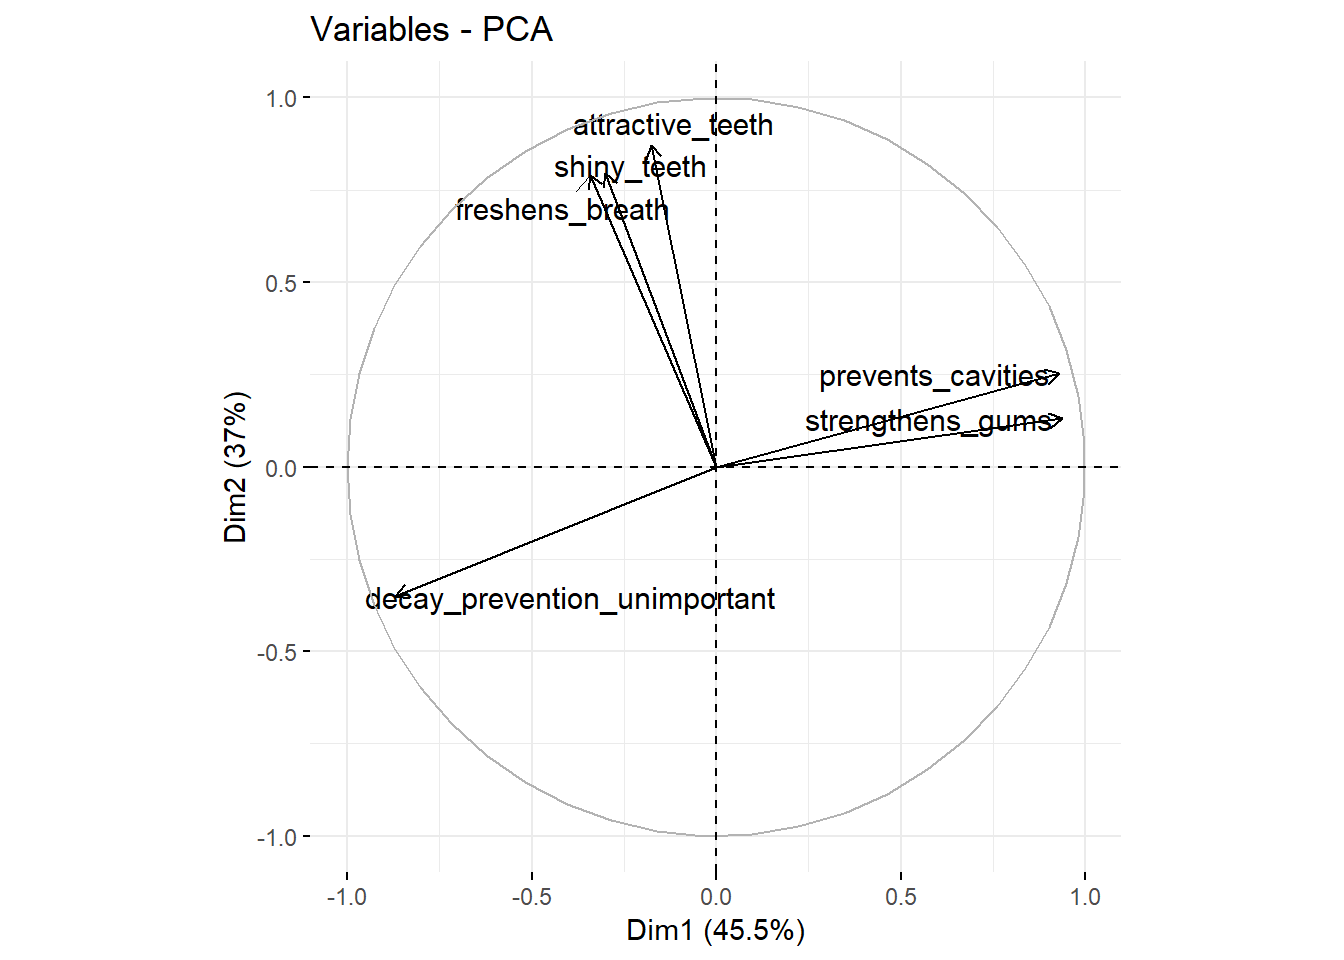
\includegraphics[width=12cm,height=8cm]{perceptual_tp_loading_plot-1.png}
\end{center}


Vemos que \fbox{attractive\_teeth}, \fbox{shiny\_teeth}, \fbox{freshens\_breath}, têm pontuações altas no segundo fator (o Dim2 do eixo X). \fbox{prevents\_cavities} e \fbox{strengthens\_gums} têm pontuações altas no segundo fator (o eixo Y Dim2) e \fbox{decay\_prevention\_unimportant} tem uma pontuação baixa nesse fator (essa variável mede a importância da prevenção da cárie).

\newpage

Também podemos adicionar as observações (os diferentes consumidores) a esse gráfico:

\begin{lstlisting}[language=R]
toothpaste %>% # pega os dados
  select(-consumer,-age,-gender) %>% # obtem as dimensoes somente
  as.data.frame() %>% # converte em data.frame object, caso contratio PCA nao aceita
  PCA(ncp = 2, graph = FALSE) %>% # faz o pca e retem 2 fatores
  fviz_pca_biplot(repel = TRUE) #faz o grafico
\end{lstlisting}


\begin{center}
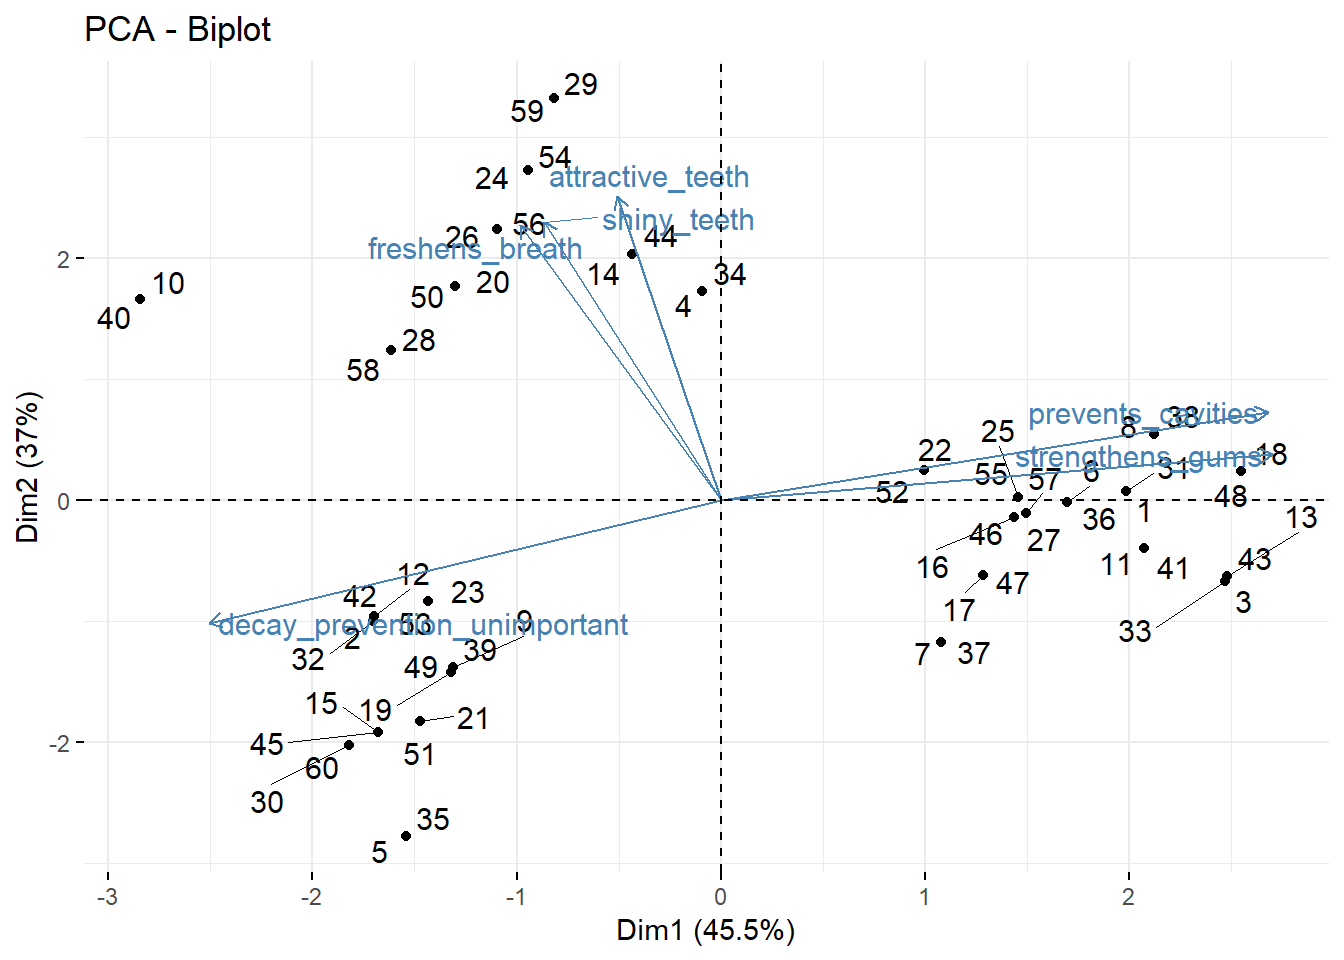
\includegraphics[width=12cm,height=8cm]{perceptual_tp_biplot-1.png}
\end{center}

Isto também é conhecido como biplot.

\newpage
\section{Análise de cluster para segmentação}

Neste capítulo, você aprenderá como realizar uma análise de cluster e uma análise discriminante linear.

Uma análise de cluster trabalha em um grupo de observações que diferem entre si em várias dimensões. Ele encontrará clusters de observações no espaço n-dimensional, de modo que a semelhança de observações dentro de clusters seja a mais alta possível e a similaridade de observações entre clusters seja a mais baixa possível. Você sempre pode executar uma análise de cluster e pode solicitar qualquer número de clusters. O número máximo de clusters é o número total de observações. Nesse caso, cada observação será um cluster, mas isso não seria um cluster muito útil. O objetivo do agrupamento em cluster é encontrar um pequeno número de clusters que possam ser descritos de forma significativa por suas pontuações médias nas n dimensões. Em outras palavras, o objetivo é encontrar diferentes 'perfis' de observações.

A análise discriminante linear tenta prever uma variável categórica com base em várias variáveis independentes contínuas ou categóricas. É semelhante à regressão logística. Nós o usaremos para prever a associação de cluster de uma observação (conforme estabelecido pela análise de cluster) com base em algumas variáveis de segmentação (ou seja, outras informações que temos sobre as observações que não serviram de entrada na análise de cluster).

Analisaremos os dados de 40 entrevistados que avaliaram a importância de vários atributos da loja ao comprar equipamentos de escritório. Usaremos a análise de cluster para encontrar agrupamentos de observações, neste caso, agrupamentos de respondentes. Esses clusters terão perfis diferentes (por exemplo, um cluster pode atribuir importância à política de preços e devoluções, o outro pode atribuir importância à variedade de opções e qualidade de serviço). Em seguida, usaremos a análise discriminante linear para testar se podemos prever a associação ao cluster (ou seja, que tipo de comprador de equipamento de escritório alguém é) com base em várias características dos entrevistados (por exemplo, sua renda).


\subsection{Dados}
\subsubsectio{Importação}

Analisaremos os dados de uma pesquisa na qual 40 entrevistados foram solicitados a avaliar a importância de vários atributos da loja ao comprar equipamentos. Faça o download dos dados aqui e importe-os para o \faRProject:

\begin{lstlisting}[language=R]
library(tidyverse) 
library(readxl)

equipment <- read_excel("segmentation_office.xlsx","SegmentationData") # Importa o arquivo Excel

\end{lstlisting}


\subsubsectio{Manipulação}
\begin{lstlisting}[language=R]
equipment

## # A tibble: 40 x 10
##    respondent_id variety_of_choi~ electronics furniture quality_of_serv~
##            <dbl>            <dbl>       <dbl>     <dbl>            <dbl>
##  1             1                8           6         6                3
##  2             2                6           3         1                4
##  3             3                6           1         2                4
##  4             4                8           3         3                4
##  5             5                4           6         3                9
##  6             6                8           4         3                5
##  7             7                7           2         2                2
##  8             8                7           5         7                2
##  9             9                7           7         5                1
## 10            10                8           4         0                4
## # ... with 30 more rows, and 5 more variables: low_prices <dbl>,
## #   return_policy <dbl>, professional <dbl>, income <dbl>, age <dbl>
 # Check out the data

\end{lstlisting}

Temos 10 colunas ou variáveis em nossos dados:
\begin{itemize}
    \item \fbox{respondent\_id} é um identificador para nossas observações
    \item Os entrevistados classificaram a importância de cada um dos seguintes atributos em uma escala de 1 a 10: \fbox{variety\_of\_choice}, \fbox{electronics}, \fbox{furniture}, \fbox{quality\_of\_service}, \fbox{low\_prices}, \fbox{return\_policy}.
    \item \fbox{professional}: 1 para profissionais, 0 para não profissionais
    \item \fbox{income}: expresso em milhares de dólares
    \item \fbox{age}
\end{itemize}

A análise de cluster tentará identificar clusters com padrões semelhantes de classificações. A análise discriminante linear preverá a associação do cluster com base nas variáveis de segmentação (\fbox{professional}, \fbox{income}, e \fbox{age}).

Como sempre, vamos fatorar as variáveis que devem ser tratadas como categóricas:

\begin{lstlisting}[language=R]
equipment <- equipment %>% 
  mutate(respondent_id = factor(respondent_id),
         professional = factor(professional, labels = c("non-professional","professional")))
\end{lstlisting}

\subsubsection{Recapitulação: importação e manipulação}

Aqui está o que fizemos até agora, em uma sequência ordenada de operações canalizadas/pipe (faça o download dos dados \href{http://users.telenet.be/samuelfranssens/tutorial_data/segmentation_office.xlsx}{aqui}):

\begin{lstlisting}[language=R]
library(tidyverse) 
library(readxl)

equipment <- read_excel("segmentation_office.xlsx","SegmentationData") %>%
  mutate(respondent_id = factor(respondent_id),
         professional = factor(professional, labels = c("non-professional","professional")))
\end{lstlisting}


\subsection{Análise de Cluster}

Primeiro, realizaremos uma análise hierárquica de cluster para encontrar o número ideal de clusters. Depois disso, realizaremos uma análise de cluster não hierárquica e solicitaremos o número de clusters considerados ideais pela análise de cluster hierárquica. As variáveis que servirão de entrada para a análise de cluster são as classificações de importância dos atributos da loja.

\subsubsection{Padronizar ou não ?}

A primeira etapa de uma análise de cluster é decidir se padronizará as variáveis de entrada. A padronização não é necessária quando as variáveis de entrada são medidas na mesma escala ou quando as variáveis de entrada são os coeficientes obtidos por uma análise conjunta. Em outros casos, a padronização é necessária.

No nosso exemplo, todas as variáveis de entrada são medidas na mesma escala e, portanto, a padronização não é necessária. Se necessário, isso pode ser feito facilmente com \fbox{mutate(newvar = scale(oldvar)))}.



\subsubsection{Cluster hierárquico}
Em seguida, criamos um novo conjunto de dados que inclui apenas as variáveis de entrada, ou seja, as classificações:

\begin{lstlisting}[language=R]
cluster.data <- equipment %>% 
  select(variety_of_choice, electronics, furniture, quality_of_service, low_prices, return_policy) # Selecione no conjunto de dados do equipamento apenas as variaveis com classificacoes padronizadas
\end{lstlisting}

Agora, podemos prosseguir com o cluster hierárquico para determinar o número ideal de clusters:

\begin{lstlisting}[language=R]
# A funcao dist() cria uma matriz de dissimilaridade do nosso conjunto de dados e deve ser o primeiro argumento para a funcao hclust().
# No argumento do metodo, voce pode especificar o metodo a ser usado para armazenamento em cluster.
hierarchical.clustering <- hclust(dist(cluster.data), method = "ward.D") 
\end{lstlisting}
\newpage

A análise de cluster é armazenada no \fbox{objeto hierarchical.clustering} e pode ser facilmente visualizada por um dendograma:

\begin{lstlisting}[language=R]
plot(hierarchical.clustering)
\end{lstlisting}



\begin{center}
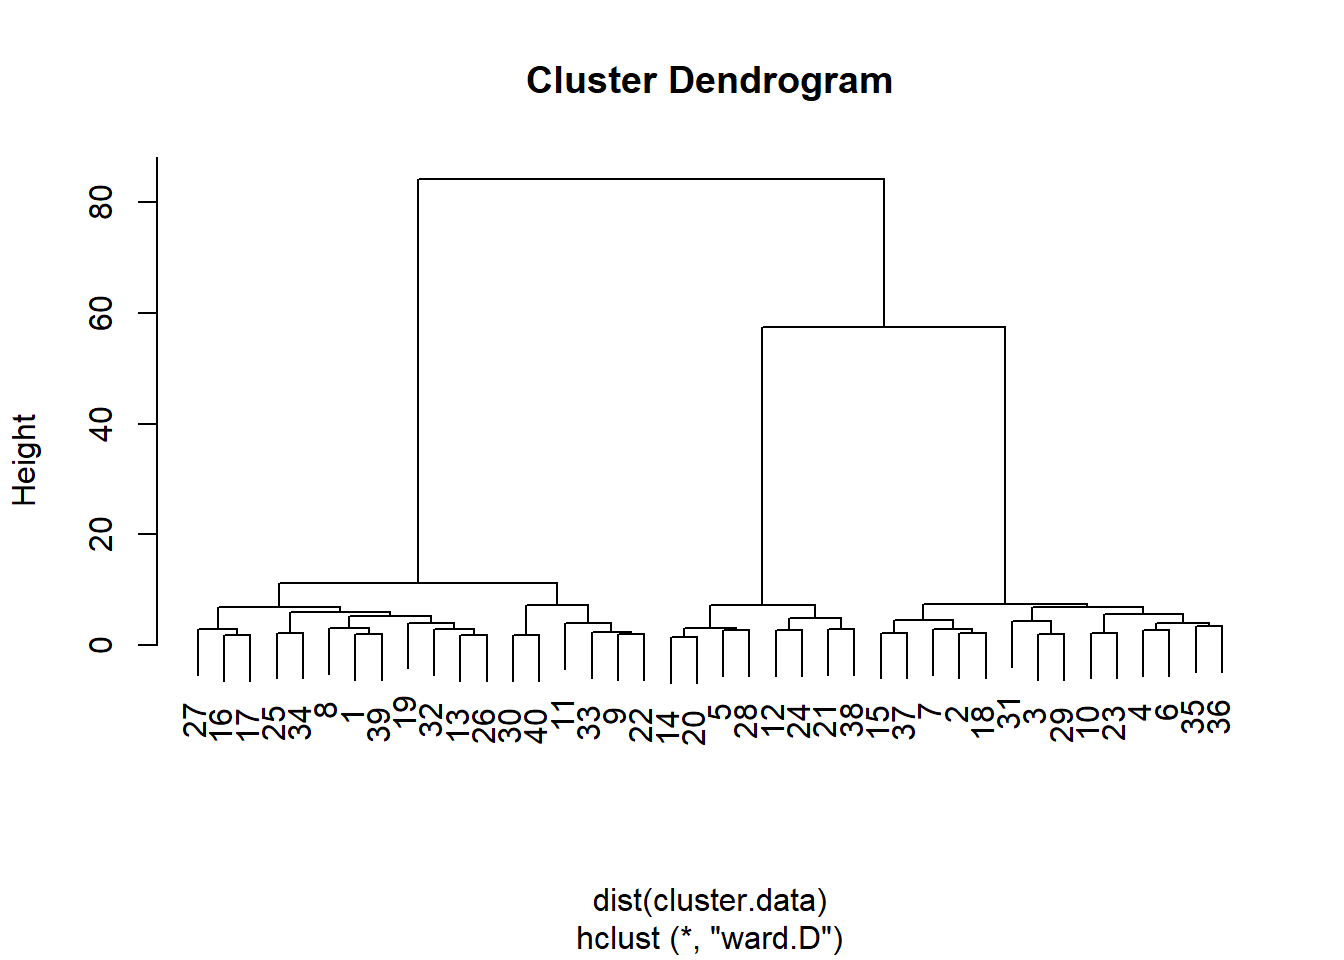
\includegraphics[width=12cm,height=8cm]{segmentation_hclust_plot-1.png}
\end{center}

A partir desse dendograma, parece que podemos dividir as observações em dois, três ou seis grupos de observações. Vamos realizar um teste formal, a regra de parada de Duda-Hart, para ver quantos clusters devemos reter. Para isso, precisamos (instalar e) carregar o \fbox{pacote NbClust}:

\begin{lstlisting}[language=R]
install.packages("NbClust")
library(NbClust)
\end{lstlisting}

A tabela de regras de parada de Duda-Hart pode ser obtida da seguinte maneira:

\begin{lstlisting}[language=R]
duda <- NbClust(cluster.data, distance = "euclidean", method = "ward.D2", max.nc = 9, index = "duda")
pseudot2 <- NbClust(cluster.data, distance = "euclidean", method = "ward.D2", max.nc = 9, index = "pseudot2")

duda$All.index

##      2      3      4      5      6      7      8      9 
## 0.3746 0.7277 0.7530 0.5062 0.4169 0.5948 0.7536 0.8615
pseudot2$All.index
##       2       3       4       5       6       7       8       9 
## 33.3846  5.9872  3.9369  5.8519  5.5945  3.4055  3.2695  1.2865
\end{lstlisting}


A sabedoria convencional para decidir o número de grupos com base na regra de parada de Duda-Hart é encontrar um dos maiores valores de Duda que corresponda a um baixo valor de pseudo-$T^2$. No entanto, você também pode solicitar o número ideal de clusters, conforme sugerido pela regra de parada:

\begin{lstlisting}[language=R]
duda$Best.nc
## Number_clusters     Value_Index 
##          3.0000          0.7277
\end{lstlisting}

Nesse caso, o número ideal é três.

\newpage

\subsection{Cluster não-hierárquico}

Agora, realizamos uma análise de cluster não hierárquica na qual solicitamos três clusters (conforme determinado pela análise de cluster hierárquica):

\begin{lstlisting}[language=R]
# existe um elemento aleatorio na analise de cluster
# isso significa que voce nem sempre obtera a mesma saida toda vez que fizer uma analise de cluster
# se voce deseja obter sempre a mesma saida, eh necessario corrigir o gerador de numeros aleatorios de R com o comando set.seed
set.seed (1)

# o argumento nstart deve ser incluido e definido como 25, mas sua explicacao esta fora do escopo deste tutorial
kmeans.clustering <- kmeans(cluster.data, 3, nstart = 25)
\end{lstlisting}

Adicione ao conjunto de \fbox{dados equipament} uma variável que indique a qual cluster uma observação pertence:

\begin{lstlisting}[language=R]
equipment <- equipment %>% 
  mutate(km.group = factor(kmeans.clustering$cluster, labels=c("cl1","cl2","cl3"))) # Fatore o indicador de cluster a partir do quadro de dados clustering k e adicione-o ao quadro de dados do equipamento.
\end{lstlisting}

Inspeciona os clusters:
\begin{lstlisting}[language=R]
equipment %>% 
  group_by(km.group) %>% # agrupado por cluster (km.group)
  summarise(count = n(), 
            variety = mean(variety_of_choice), 
            electronics = mean(electronics), 
            furniture = mean(furniture), 
            service = mean(quality_of_service), 
            prices = mean(low_prices), 
            return = mean(return_policy)) #Em seguida, pergunte pelo número de entrevistados e pelos meios das classificações.
            
## # A tibble: 3 x 8
##   km.group count variety electronics furniture service prices return
##   <fct>    <int>   <dbl>       <dbl>     <dbl>   <dbl>  <dbl>  <dbl>
## 1 cl1          8    5           4.38      1.75    8.5    2.5    4.38
## 2 cl2         18    9.11        6.06      5.78    2.39   3.67   3.17
## 3 cl3         14    6.93        2.79      1.43    3.5    8.29   6.29
\end{lstlisting}

Vemos que:
\begin{itemize}
    \item o cluster 1 atribui mais importância (do que outros clusters) à qualidade do serviço
    \item o cluster 2 atribui mais importância à variedade de opções
    \item o cluster 3 atribui mais importância a preços baixos
\end{itemize}

Também podemos testar se há diferenças significativas entre os clusters, por exemplo, na variedade de opções. Para isso, usamos uma ANOVA unidirecional:

\begin{lstlisting}[language=R]
# remotes::install_github("samuelfranssens/type3anova") # para instalar o pacote type3anova.
# Voce precisa do pacote de controles remotos para isso e o pacote para carro precisa ser instalado para que o pacote type3anova funcione

library(type3anova)
type3anova(lm(variety_of_choice ~ km.group, data=equipment))

## # A tibble: 3 x 6
##   term            ss   df1   df2      f    pvalue
##   <chr>        <dbl> <dbl> <int>  <dbl>     <dbl>
## 1 (Intercept) 1757.      1    37 1335.   1.24e-30
## 2 km.group     101.      2    37   38.5  9.20e-10
## 3 Residuals     48.7    37    37   NA   NA
\end{lstlisting}

Existem diferenças significativas entre os clusters em importância associadas à variedade de opções, e isso faz sentido porque o objetivo da análise de clusters é maximizar as diferenças entre os clusters. Vamos acompanhar isso com o HSD de Tukey para ver exatamente quais meios diferem um do outro:

\newpage
\begin{lstlisting}[language=R]
TukeyHSD(aov(variety_of_choice ~ km.group, data=equipment), 
         "km.group") # O primeiro argumento eh um objeto "aov", o segundo eh a nossa variavel independente.
         
##   Tukey multiple comparisons of means
##     95% family-wise confidence level
## 
## Fit: aov(formula = variety_of_choice ~ km.group, data = equipment)
## 
## $km.group
##              diff        lwr       upr     p adj
## cl2-cl1  4.111111  2.9208248  5.301397 0.0000000
## cl3-cl1  1.928571  0.6870668  3.170076 0.0015154
## cl3-cl2 -2.182540 -3.1807470 -1.184332 0.0000145

\end{lstlisting}
Vemos que em todos os meios, a diferença é significativa.

\subsection{LDA Canônico}

Na vida real, geralmente não sabemos o que os potenciais compradores consideram importante, mas temos uma ideia, por exemplo, de sua renda, idade e status profissional. Portanto, seria útil testar quão bem podemos prever a associação ao cluster (perfil de classificações de importância) com base nas características dos respondentes (renda, idade, profissional), que também são chamados de variáveis de segmentação. A fórmula preditiva poderia então ser usada para prever a associação ao cluster de novos compradores em potencial. Para encontrar a fórmula correta, usamos a análise discriminante linear (LDA). Mas primeiro vamos dar uma olhada nas médias de income, age, e professional por cluster:

\begin{lstlisting}[language=R]

equipment %>% 
  group_by(km.group) %>% # Agrupar equipamentos por cluster.
  summarize(income = mean(income), 
            age = mean(age), 
            professional = mean(as.numeric(professional)-1)) 
            
## # A tibble: 3 x 4
##   km.group income   age professional
##   <fct>     <dbl> <dbl>        <dbl>
## 1 cl1        47.5  49          0.75 
## 2 cl2        48.3  44.2        0.333
## 3 cl3        32.1  30.9        0.5
# Nao podemos assumir a media do profissional porque e uma variavel fator. 
# Pedimos, portanto, que R o trate como uma variavel numerica.
# acessado por $class, para os new_data com base na formula do LDA com base nos dados antigos (use o LDA onde CV = FALSE).

#visualiza as predicoes

new_data
## # A tibble: 4 x 4
##   income   age professional     prediction
##    <dbl> <dbl> <chr>            <fct>     
## 1     65    20 professional     cluster 3 
## 2     65    35 non-professional cluster 2 
## 3     35    45 non-professional cluster 2 
## 4     35    60 professional     cluster 1
\end{lstlisting}

\newpage

\section{Análise Conjunta}

Neste capítulo, você aprenderá como realizar uma análise conjunta. A análise conjunta começa a partir de uma pesquisa na qual as pessoas avaliam ou escolhem entre produtos (por exemplo, carros) que diferem em vários atributos (por exemplo, segurança, eficiência de combustível, conforto etc.). A partir dessas classificações ou escolhas, a análise determina o valor que as pessoas atribuem aos diferentes atributos do produto (por exemplo, quanto peso as pessoas atribuem à segurança ao escolher entre carros). Essas informações podem ser usadas no desenvolvimento de produtos.


\subsection{Dados}

\subsubsection{Importação}


Analisaremos os dados de uma pesquisa em que 15 consumidores foram convidados a avaliar dez sorvetes. Cada sorvete tinha um 'perfil' diferente, ou seja, uma combinação diferente de níveis de quatro atributos: sabor (framboesa, chocolate, morango, manga, baunilha), embalagem (waffle caseiro, casquinha, caneca), leve (com pouca gordura ou não) e orgânico (orgânico ou não). Todos os 15 entrevistados classificaram os dez perfis, fornecendo uma pontuação entre 1 e 10.

Usamos os dados fornecidos pelo \href{https://bookdown.org/content/1340/www.xlstat.com}{www.xlstat.com}, descritos em seu \href{https://help.xlstat.com/customer/en/portal/articles/2062346-conjoint-analysis-in-excel-tutorial?b_id=9283}{tutorial} sobre como fazer análises conjuntas no Excel. Faça o download dos dados \href{http://users.telenet.be/samuelfranssens/tutorial_data/icecream.xlsx}{aqui.}

\begin{lstlisting}[language=R]
library(tidyverse)
library(readxl)

icecream <- read_excel("icecream.xlsx") # Nao eh necessario incluir o argumento da planilha quando houver apenas uma planilha no arquivo do Excel
\end{lstlisting}

\subsubsection{Manipulação}

\begin{lstlisting}[language=R]
icecream

## # A tibble: 10 x 20
##    Observations Flavor Packaging Light Organic `Individual 1`
##    <chr>        <chr>  <chr>     <chr> <chr>            <dbl>
##  1 Profile 1    Raspb~ Homemade~ No l~ Not or~              1
##  2 Profile 2    Choco~ Cone      No l~ Organic              4
##  3 Profile 3    Raspb~ Pint      Low ~ Organic              2
##  4 Profile 4    Straw~ Pint      No l~ Organic              7
##  5 Profile 5    Straw~ Cone      Low ~ Not or~              9
##  6 Profile 6    Choco~ Homemade~ No l~ Not or~              3
##  7 Profile 7    Vanil~ Pint      Low ~ Not or~              5
##  8 Profile 8    Mango  Homemade~ Low ~ Organic             10
##  9 Profile 9    Mango  Pint      No l~ Not or~              6
## 10 Profile 10   Vanil~ Homemade~ No l~ Organic              8
## # ... with 14 more variables: `Individual 2` <dbl>, `Individual 3` <dbl>,
## #   `Individual 4` <dbl>, `Individual 5` <dbl>, `Individual 6` <dbl>,
## #   `Individual 7` <dbl>, `Individual 8` <dbl>, `Individual 9` <dbl>,
## #   `Individual 10` <dbl>, `Individual 11` <dbl>, `Individual 12` <dbl>,
## #   `Individual 13` <dbl>, `Individual 14` <dbl>, `Individual 15` <dbl>

\end{lstlisting}


Quando inspecionamos os dados, vemos que temos uma coluna para cada entrevistado. Essa é uma maneira incomum de armazenar dados (normalmente temos uma linha por respondente), então vamos reestruturar nosso conjunto de dados com a função de coleta (como fizemos \href{https://bookdown.org/content/1340/rmanova.html#rmanova}{anteriormente}):

\begin{lstlisting}[language=R]
icecream <- icecream %>% 
  gather(respondent, rating, starts_with("Individual")) %>% # o entrevistado acompanha o respondente, a classificacao armazena as classificacoes do entrevistado e queremos empilhar todas as variaveis que comecam com Individual
  rename("profile" = "Observations") %>% # renomeia Observations para profile
  mutate(profile = factor(profile), respondent = factor(respondent),  # fatorar identificadores
         Flavor = factor(Flavor), Packaging = factor(Packaging), Light = factor(Light), Organic = factor(Organic)) # fatorar os atributos do sorvete


# Amplo conjunto de dados: uma linha por unidade de observacao (aqui: perfil) e varias colunas para as diferentes observacoes (aqui: respondentes)
# Conjunto de dados longo: uma linha por observacao (aqui: combinacao de perfil x respondente)

# Converter de grande para longo significa que estamos empilhando varias colunas umas sobre as outras. Para isso, precisamos de uma variavel extra para acompanhar qual coluna estamos lidando.
# A funcao de coleta converte conjuntos de dados de amplos para longos.
# O primeiro argumento (respondente) nos dira com qual coluna estamos lidando. Essa eh a variavel que armazenara os nomes das colunas que estamos empilhando.
# O segundo argumento (classificacao) armazenara as colunas reais empilhadas umas sobre as outras.
# Os argumentos a seguir (todas as variaveis com nomes que comecam com Individual) sao as colunas que queremos empilhar.

icecream

## # A tibble: 150 x 7
##    profile   Flavor    Packaging     Light    Organic   respondent  rating
##    <fct>     <fct>     <fct>         <fct>    <fct>     <fct>        <dbl>
##  1 Profile 1 Raspberry Homemade waf~ No low ~ Not orga~ Individual~      1
##  2 Profile 2 Chocolate Cone          No low ~ Organic   Individual~      4
##  3 Profile 3 Raspberry Pint          Low fat  Organic   Individual~      2
##  4 Profile 4 Strawber~ Pint          No low ~ Organic   Individual~      7
##  5 Profile 5 Strawber~ Cone          Low fat  Not orga~ Individual~      9
##  6 Profile 6 Chocolate Homemade waf~ No low ~ Not orga~ Individual~      3
##  7 Profile 7 Vanilla   Pint          Low fat  Not orga~ Individual~      5
##  8 Profile 8 Mango     Homemade waf~ Low fat  Organic   Individual~     10
##  9 Profile 9 Mango     Pint          No low ~ Not orga~ Individual~      6
## 10 Profile ~ Vanilla   Homemade waf~ No low ~ Organic   Individual~      8
## # ... with 140 more rows
\end{lstlisting}

É melhor usar o Visualizador aqui (clique duas vezes no \fbox{icecream} objeto no painel Ambiente ou digite \fbox{View(icecream))} para ver que existem dez linhas (10 perfis) por respondente agora.

As demais variáveis são:

\begin{itemize}
    \item \fbox{profile} é um identificador para os diferentes sorvetes
    \item \fbox{Flavor}, \fbox{Packaging}, \fbox{Light}, \fbox{Organic} são os quatro atributos que compõem o perfil de um sorvete
\end{itemize}

\subsubsection{Recapitulando: importação e manipulação}

Aqui está o que fizemos até agora, em uma sequência ordenada de operações canalizadas (faça o download dos dados \href{http://users.telenet.be/samuelfranssens/tutorial_data/icecream.xlsx}{aqui}:)
\begin{lstlisting}[language=R]
library(tidyverse)
library(readxl)

icecream <- read_excel("icecream.xlsx") %>% 
  gather(respondent, rating, starts_with("Individual")) %>% # o entrevistado acompanha o respondente, a classificacao armazena as classificacoes do entrevistado e queremos empilhar todas as variaveis que comecam com Individual
  rename("profile" = "Observations") %>% 
  mutate(profile = factor(profile), respondent = factor(respondent),
         Flavor = factor(Flavor), Packaging = factor(Packaging), Light = factor(Light), Organic = factor(Organic))
\end{lstlisting}


\subsection{Design de experimentos}

Quando inspecionamos nosso conjunto de dados, vemos que o \fbox{flavor} possui 5 níveis (framboesa, chocolate, morango, manga, baunilha), \fbox{packaging} possui 3 níveis (waffle caseiro, cone, cerveja), a \fbox{Light} possui 2 níveis (baixo teor de gordura versus não), e \fbox{Organic} tem 2 níveis (orgânico vs. não). O objetivo de uma análise conjunta é estimar até que ponto cada nível de atributo afeta a classificação do sorvete.

Para fazer isso, o fabricante de sorvete poderia criar 5×3×2x2 = 60 sorvetes diferentes e peça às pessoas para avaliarem tudo isso. Isso fornecerá ao fabricante uma boa estimativa da importância de cada atributo e de todas as possíveis interações. No entanto, classificar 60 sorvetes é difícil para os participantes e um estudo tão grande seria caro para o fabricante financiar. Na prática, os pesquisadores nessa situação solicitarão que as pessoas classifiquem um subconjunto desses 60 sorvetes. Nesta seção, discutiremos como selecionar um subconjunto (por exemplo, 10 sorvetes) de todas as combinações possíveis de nível de atributo (ou seja, 60 sorvetes) que ainda nos permitirão obter boas estimativas dos efeitos mais importantes.

No conjunto de dados, já temos as classificações para dez perfis, portanto a decisão de quais sorvetes para teste já foi tomada. No entanto, vamos desconsiderar o fato de já termos os dados e considerar as decisões que precisam ser tomadas antes da coleta de dados. Em outras palavras, vamos discutir como passamos de um \textit{fatorial completo} (todas as 60 combinações) para um design \textit{fracionário} (menos de 60 combinações).

A função doe (projeto de experimentos) do \fbox{pacote radiant} nos ajudará a decidir sobre os projetos de estudo. \fbox{Radiant} é um \href{https://radiant-rstats.github.io/docs/index.html}{pacote do \faRProject para business analytics.}

A discussão a seguir da função doe é baseada na discussão da \fbox{Radiant} sobre essa função.

\begin{lstlisting}[language=R]
install.packages("radiant")
library(radiant)
\end{lstlisting}


Para usar a doe, precisamos inserir as informações sobre nossos atributos e seus níveis de uma maneira específica:

\begin{lstlisting}[language=R]
# attribute1, attribute2, etc. sao vetores com um elemento no qual fornecemos primeiro o nome do atributo seguido por um ponto e virgula e depois fornecemos todos os niveis dos atributos separados por ponto e virgula
attribute1 <- "Flavor; Raspberry; Chocolate; Strawberry; Mango; Vanilla"
attribute2 <- "Package; Homemade waffle; Cone; Pint"
attribute3 <- "Light; Low fat; No low fat"
attribute4 <- "Organic; Organic; Not organic"

# agora combine esses diferentes atributos em um vetor com c()
attributes <- c(attribute1, attribute2, attribute3, attribute4)
\end{lstlisting}

Agora podemos pedir possíveis projetos experimentais:

\begin{lstlisting}[language=R]
summary(doe(attributes, seed = 123)) # Seed: fixa o gerador de numeros aleatorios

## Experimental design
## # trials for partial factorial: 60 
## # trials for full factorial   : 60 
## Random seed                   : 123 
## 
## Attributes and levels:
## Flavor: Raspberry, Chocolate, Strawberry, Mango, Vanilla 
## Package: Homemade_waffle, Cone, Pint 
## Light: Low_fat, No_low_fat 
## Organic: Organic, Not_organic 
## 
## Design efficiency:
##  Trials D-efficiency Balanced
##       9        0.105    FALSE
##      10        0.389    FALSE
##      11        0.411    FALSE
##      12        0.614    FALSE
##      13        0.542    FALSE
##      14        0.479    FALSE
##      15        0.762    FALSE
##      16        0.738    FALSE
##      17        0.748    FALSE
##      18        0.756    FALSE
##      19        0.644    FALSE
##      20        0.895    FALSE
##      21        0.848    FALSE
##      22        0.833    FALSE
##      23        0.790    FALSE
##      24        0.827    FALSE
##      25        0.787    FALSE
##      26        0.768    FALSE
##      27        0.759    FALSE
##      28        0.736    FALSE
##      29        0.702    FALSE
##      30        0.984     TRUE
##      31        0.952    FALSE
##      32        0.933    FALSE
##      33        0.928    FALSE
##      34        0.900    FALSE
##      35        0.871    FALSE
##      36        0.893    FALSE
##      37        0.866    FALSE
##      38        0.843    FALSE
##      39        0.836    FALSE
##      40        0.922    FALSE
##      41        0.899    FALSE
##      42        0.904    FALSE
##      43        0.882    FALSE
##      44        0.861    FALSE
##      45        0.949    FALSE
##      46        0.919    FALSE
##      47        0.912    FALSE
##      48        0.911    FALSE
##      49        0.891    FALSE
##      50        0.959    FALSE
##      51        0.939    FALSE
##      52        0.944    FALSE
##      53        0.925    FALSE
##      54        0.924    FALSE
##      55        0.906    FALSE
##      56        0.902    FALSE
##      57        0.884    FALSE
##      58        0.872    FALSE
##      59        0.855    FALSE
##      60        1.000     TRUE
## 
## Partial factorial design correlations:
##         Flavor Package Light Organic
## Flavor       1       0     0       0
## Package      0       1     0       0
## Light        0       0     1       0
## Organic      0       0     0       1
## 
## Partial factorial design:
##  trial     Flavor         Package      Light     Organic
##      1  Raspberry Homemade_waffle    Low_fat     Organic
##      2  Raspberry Homemade_waffle    Low_fat Not_organic
##      3  Raspberry Homemade_waffle No_low_fat     Organic
##      4  Raspberry Homemade_waffle No_low_fat Not_organic
##      5  Raspberry            Cone    Low_fat     Organic
##      6  Raspberry            Cone    Low_fat Not_organic
##      7  Raspberry            Cone No_low_fat     Organic
##      8  Raspberry            Cone No_low_fat Not_organic
##      9  Raspberry            Pint    Low_fat     Organic
##     10  Raspberry            Pint    Low_fat Not_organic
##     11  Raspberry            Pint No_low_fat     Organic
##     12  Raspberry            Pint No_low_fat Not_organic
##     13  Chocolate Homemade_waffle    Low_fat     Organic
##     14  Chocolate Homemade_waffle    Low_fat Not_organic
##     15  Chocolate Homemade_waffle No_low_fat     Organic
##     16  Chocolate Homemade_waffle No_low_fat Not_organic
##     17  Chocolate            Cone    Low_fat     Organic
##     18  Chocolate            Cone    Low_fat Not_organic
##     19  Chocolate            Cone No_low_fat     Organic
##     20  Chocolate            Cone No_low_fat Not_organic
##     21  Chocolate            Pint    Low_fat     Organic
##     22  Chocolate            Pint    Low_fat Not_organic
##     23  Chocolate            Pint No_low_fat     Organic
##     24  Chocolate            Pint No_low_fat Not_organic
##     25 Strawberry Homemade_waffle    Low_fat     Organic
##     26 Strawberry Homemade_waffle    Low_fat Not_organic
##     27 Strawberry Homemade_waffle No_low_fat     Organic
##     28 Strawberry Homemade_waffle No_low_fat Not_organic
##     29 Strawberry            Cone    Low_fat     Organic
##     30 Strawberry            Cone    Low_fat Not_organic
##     31 Strawberry            Cone No_low_fat     Organic
##     32 Strawberry            Cone No_low_fat Not_organic
##     33 Strawberry            Pint    Low_fat     Organic
##     34 Strawberry            Pint    Low_fat Not_organic
##     35 Strawberry            Pint No_low_fat     Organic
##     36 Strawberry            Pint No_low_fat Not_organic
##     37      Mango Homemade_waffle    Low_fat     Organic
##     38      Mango Homemade_waffle    Low_fat Not_organic
##     39      Mango Homemade_waffle No_low_fat     Organic
##     40      Mango Homemade_waffle No_low_fat Not_organic
##     41      Mango            Cone    Low_fat     Organic
##     42      Mango            Cone    Low_fat Not_organic
##     43      Mango            Cone No_low_fat     Organic
##     44      Mango            Cone No_low_fat Not_organic
##     45      Mango            Pint    Low_fat     Organic
##     46      Mango            Pint    Low_fat Not_organic
##     47      Mango            Pint No_low_fat     Organic
##     48      Mango            Pint No_low_fat Not_organic
##     49    Vanilla Homemade_waffle    Low_fat     Organic
##     50    Vanilla Homemade_waffle    Low_fat Not_organic
##     51    Vanilla Homemade_waffle No_low_fat     Organic
##     52    Vanilla Homemade_waffle No_low_fat Not_organic
##     53    Vanilla            Cone    Low_fat     Organic
##     54    Vanilla            Cone    Low_fat Not_organic
##     55    Vanilla            Cone No_low_fat     Organic
##     56    Vanilla            Cone No_low_fat Not_organic
##     57    Vanilla            Pint    Low_fat     Organic
##     58    Vanilla            Pint    Low_fat Not_organic
##     59    Vanilla            Pint No_low_fat     Organic
##     60    Vanilla            Pint No_low_fat Not_organic
## 
## Full factorial design:
##  trial     Flavor         Package      Light     Organic
##      1  Raspberry Homemade_waffle    Low_fat     Organic
##      2  Raspberry Homemade_waffle    Low_fat Not_organic
##      3  Raspberry Homemade_waffle No_low_fat     Organic
##      4  Raspberry Homemade_waffle No_low_fat Not_organic
##      5  Raspberry            Cone    Low_fat     Organic
##      6  Raspberry            Cone    Low_fat Not_organic
##      7  Raspberry            Cone No_low_fat     Organic
##      8  Raspberry            Cone No_low_fat Not_organic
##      9  Raspberry            Pint    Low_fat     Organic
##     10  Raspberry            Pint    Low_fat Not_organic
##     11  Raspberry            Pint No_low_fat     Organic
##     12  Raspberry            Pint No_low_fat Not_organic
##     13  Chocolate Homemade_waffle    Low_fat     Organic
##     14  Chocolate Homemade_waffle    Low_fat Not_organic
##     15  Chocolate Homemade_waffle No_low_fat     Organic
##     16  Chocolate Homemade_waffle No_low_fat Not_organic
##     17  Chocolate            Cone    Low_fat     Organic
##     18  Chocolate            Cone    Low_fat Not_organic
##     19  Chocolate            Cone No_low_fat     Organic
##     20  Chocolate            Cone No_low_fat Not_organic
##     21  Chocolate            Pint    Low_fat     Organic
##     22  Chocolate            Pint    Low_fat Not_organic
##     23  Chocolate            Pint No_low_fat     Organic
##     24  Chocolate            Pint No_low_fat Not_organic
##     25 Strawberry Homemade_waffle    Low_fat     Organic
##     26 Strawberry Homemade_waffle    Low_fat Not_organic
##     27 Strawberry Homemade_waffle No_low_fat     Organic
##     28 Strawberry Homemade_waffle No_low_fat Not_organic
##     29 Strawberry            Cone    Low_fat     Organic
##     30 Strawberry            Cone    Low_fat Not_organic
##     31 Strawberry            Cone No_low_fat     Organic
##     32 Strawberry            Cone No_low_fat Not_organic
##     33 Strawberry            Pint    Low_fat     Organic
##     34 Strawberry            Pint    Low_fat Not_organic
##     35 Strawberry            Pint No_low_fat     Organic
##     36 Strawberry            Pint No_low_fat Not_organic
##     37      Mango Homemade_waffle    Low_fat     Organic
##     38      Mango Homemade_waffle    Low_fat Not_organic
##     39      Mango Homemade_waffle No_low_fat     Organic
##     40      Mango Homemade_waffle No_low_fat Not_organic
##     41      Mango            Cone    Low_fat     Organic
##     42      Mango            Cone    Low_fat Not_organic
##     43      Mango            Cone No_low_fat     Organic
##     44      Mango            Cone No_low_fat Not_organic
##     45      Mango            Pint    Low_fat     Organic
##     46      Mango            Pint    Low_fat Not_organic
##     47      Mango            Pint No_low_fat     Organic
##     48      Mango            Pint No_low_fat Not_organic
##     49    Vanilla Homemade_waffle    Low_fat     Organic
##     50    Vanilla Homemade_waffle    Low_fat Not_organic
##     51    Vanilla Homemade_waffle No_low_fat     Organic
##     52    Vanilla Homemade_waffle No_low_fat Not_organic
##     53    Vanilla            Cone    Low_fat     Organic
##     54    Vanilla            Cone    Low_fat Not_organic
##     55    Vanilla            Cone No_low_fat     Organic
##     56    Vanilla            Cone No_low_fat Not_organic
##     57    Vanilla            Pint    Low_fat     Organic
##     58    Vanilla            Pint    Low_fat Not_organic
##     59    Vanilla            Pint No_low_fat     Organic
##     60    Vanilla            Pint No_low_fat Not_organic
\end{lstlisting}

Observe a saída no cabeçalho \fbox{Design efficiency}. Mostra 52 linhas. As linhas representam projetos experimentais com diferentes números de \fbox{Trials} ou diferentes números de sorvetes (ou seja, combinações de nível de atributo) que seriam testados. Uma palavra melhor para julgamento é perfil. Para cada projeto experimental, ele mostra a \fbox{D-efficiency} do projeto - uma medida de como poderemos estimar com clareza os efeitos do interesse após a execução do experimento (pontuações mais altas são melhores) - e se o projeto está ou não equilibrado - se cada nível está incluído no mesmo número de tentativas ou perfis. Idealmente, procuramos projetos balanceados com alta \fbox{D-efficiency} (acima de 0,80 é considerado razoável). Temos dois candidatos, um delineamento experimental com 60 perfis, que é apenas o delineamento fatorial completo ou um delineamento com 30 perfis. Vamos dar uma olhada no design com 30 perfis:

\begin{lstlisting}[language=R]
summary(doe(attributes, seed = 123, trials = 30))

## Experimental design
## # trials for partial factorial: 30 
## # trials for full factorial   : 60 
## Random seed                   : 123 
## 
## Attributes and levels:
## Flavor: Raspberry, Chocolate, Strawberry, Mango, Vanilla 
## Package: Homemade_waffle, Cone, Pint 
## Light: Low_fat, No_low_fat 
## Organic: Organic, Not_organic 
## 
## Design efficiency:
##  Trials D-efficiency Balanced
##      30        0.984     TRUE
## 
## Partial factorial design correlations:
##         Flavor Package  Light Organic
## Flavor       1       0  0.000   0.000
## Package      0       1  0.000   0.000
## Light        0       0  1.000  -0.105
## Organic      0       0 -0.105   1.000
## 
## Partial factorial design:
##  trial     Flavor         Package      Light     Organic
##      1  Raspberry Homemade_waffle    Low_fat     Organic
##      4  Raspberry Homemade_waffle No_low_fat Not_organic
##      6  Raspberry            Cone    Low_fat Not_organic
##      7  Raspberry            Cone No_low_fat     Organic
##     10  Raspberry            Pint    Low_fat Not_organic
##     11  Raspberry            Pint No_low_fat     Organic
##     13  Chocolate Homemade_waffle    Low_fat     Organic
##     14  Chocolate Homemade_waffle    Low_fat Not_organic
##     19  Chocolate            Cone No_low_fat     Organic
##     20  Chocolate            Cone No_low_fat Not_organic
##     22  Chocolate            Pint    Low_fat Not_organic
##     23  Chocolate            Pint No_low_fat     Organic
##     26 Strawberry Homemade_waffle    Low_fat Not_organic
##     28 Strawberry Homemade_waffle No_low_fat Not_organic
##     29 Strawberry            Cone    Low_fat     Organic
##     32 Strawberry            Cone No_low_fat Not_organic
##     33 Strawberry            Pint    Low_fat     Organic
##     35 Strawberry            Pint No_low_fat     Organic
##     39      Mango Homemade_waffle No_low_fat     Organic
##     40      Mango Homemade_waffle No_low_fat Not_organic
##     41      Mango            Cone    Low_fat     Organic
##     42      Mango            Cone    Low_fat Not_organic
##     46      Mango            Pint    Low_fat Not_organic
##     47      Mango            Pint No_low_fat     Organic
##     49    Vanilla Homemade_waffle    Low_fat     Organic
##     51    Vanilla Homemade_waffle No_low_fat     Organic
##     53    Vanilla            Cone    Low_fat     Organic
##     56    Vanilla            Cone No_low_fat Not_organic
##     58    Vanilla            Pint    Low_fat Not_organic
##     60    Vanilla            Pint No_low_fat Not_organic
## 
## Full factorial design:
##  trial     Flavor         Package      Light     Organic
##      1  Raspberry Homemade_waffle    Low_fat     Organic
##      2  Raspberry Homemade_waffle    Low_fat Not_organic
##      3  Raspberry Homemade_waffle No_low_fat     Organic
##      4  Raspberry Homemade_waffle No_low_fat Not_organic
##      5  Raspberry            Cone    Low_fat     Organic
##      6  Raspberry            Cone    Low_fat Not_organic
##      7  Raspberry            Cone No_low_fat     Organic
##      8  Raspberry            Cone No_low_fat Not_organic
##      9  Raspberry            Pint    Low_fat     Organic
##     10  Raspberry            Pint    Low_fat Not_organic
##     11  Raspberry            Pint No_low_fat     Organic
##     12  Raspberry            Pint No_low_fat Not_organic
##     13  Chocolate Homemade_waffle    Low_fat     Organic
##     14  Chocolate Homemade_waffle    Low_fat Not_organic
##     15  Chocolate Homemade_waffle No_low_fat     Organic
##     16  Chocolate Homemade_waffle No_low_fat Not_organic
##     17  Chocolate            Cone    Low_fat     Organic
##     18  Chocolate            Cone    Low_fat Not_organic
##     19  Chocolate            Cone No_low_fat     Organic
##     20  Chocolate            Cone No_low_fat Not_organic
##     21  Chocolate            Pint    Low_fat     Organic
##     22  Chocolate            Pint    Low_fat Not_organic
##     23  Chocolate            Pint No_low_fat     Organic
##     24  Chocolate            Pint No_low_fat Not_organic
##     25 Strawberry Homemade_waffle    Low_fat     Organic
##     26 Strawberry Homemade_waffle    Low_fat Not_organic
##     27 Strawberry Homemade_waffle No_low_fat     Organic
##     28 Strawberry Homemade_waffle No_low_fat Not_organic
##     29 Strawberry            Cone    Low_fat     Organic
##     30 Strawberry            Cone    Low_fat Not_organic
##     31 Strawberry            Cone No_low_fat     Organic
##     32 Strawberry            Cone No_low_fat Not_organic
##     33 Strawberry            Pint    Low_fat     Organic
##     34 Strawberry            Pint    Low_fat Not_organic
##     35 Strawberry            Pint No_low_fat     Organic
##     36 Strawberry            Pint No_low_fat Not_organic
##     37      Mango Homemade_waffle    Low_fat     Organic
##     38      Mango Homemade_waffle    Low_fat Not_organic
##     39      Mango Homemade_waffle No_low_fat     Organic
##     40      Mango Homemade_waffle No_low_fat Not_organic
##     41      Mango            Cone    Low_fat     Organic
##     42      Mango            Cone    Low_fat Not_organic
##     43      Mango            Cone No_low_fat     Organic
##     44      Mango            Cone No_low_fat Not_organic
##     45      Mango            Pint    Low_fat     Organic
##     46      Mango            Pint    Low_fat Not_organic
##     47      Mango            Pint No_low_fat     Organic
##     48      Mango            Pint No_low_fat Not_organic
##     49    Vanilla Homemade_waffle    Low_fat     Organic
##     50    Vanilla Homemade_waffle    Low_fat Not_organic
##     51    Vanilla Homemade_waffle No_low_fat     Organic
##     52    Vanilla Homemade_waffle No_low_fat Not_organic
##     53    Vanilla            Cone    Low_fat     Organic
##     54    Vanilla            Cone    Low_fat Not_organic
##     55    Vanilla            Cone No_low_fat     Organic
##     56    Vanilla            Cone No_low_fat Not_organic
##     57    Vanilla            Pint    Low_fat     Organic
##     58    Vanilla            Pint    Low_fat Not_organic
##     59    Vanilla            Pint No_low_fat     Organic
##     60    Vanilla            Pint No_low_fat Not_organic
\end{lstlisting}


Em Projeto fatorial parcial (ou projeto fatorial fracionário), encontramos os perfis que poderíamos executar em um experimento com 30 em vez de 60 perfis. Sob correlações parciais do projeto fatorial, vemos que dois atributos estão correlacionados, a saber, \fbox{Light} e \fbox{Organic} ($r = -0,105$). Esse sempre será o caso em projetos fatoriais fracionários. Isso significa que algumas combinações de níveis de atributo serão mais prevalentes que outras. Somente em um planejamento fatorial completo todos os atributos serão não correlacionados ou ortogonais.

Um design possível com apenas 10 perfis seria desequilibrado e teria a seguinte aparência:

\begin{lstlisting}[language=R]
summary(doe(attributes, seed = 123, trials = 10))

## Experimental design
## # trials for partial factorial: 10 
## # trials for full factorial   : 60 
## Random seed                   : 123 
## 
## Attributes and levels:
## Flavor: Raspberry, Chocolate, Strawberry, Mango, Vanilla 
## Package: Homemade_waffle, Cone, Pint 
## Light: Low_fat, No_low_fat 
## Organic: Organic, Not_organic 
## 
## Design efficiency:
##  Trials D-efficiency Balanced
##      10        0.389    FALSE
## 
## Partial factorial design correlations:
##         Flavor Package Light Organic
## Flavor   1.000   0.121 0.000   0.000
## Package  0.121   1.000 0.000   0.000
## Light    0.000   0.000 1.000   0.309
## Organic  0.000   0.000 0.309   1.000
## 
## Partial factorial design:
##  trial     Flavor         Package      Light     Organic
##      4  Raspberry Homemade_waffle No_low_fat Not_organic
##      5  Raspberry            Cone    Low_fat     Organic
##     20  Chocolate            Cone No_low_fat Not_organic
##     21  Chocolate            Pint    Low_fat     Organic
##     25 Strawberry Homemade_waffle    Low_fat     Organic
##     36 Strawberry            Pint No_low_fat Not_organic
##     39      Mango Homemade_waffle No_low_fat     Organic
##     46      Mango            Pint    Low_fat Not_organic
##     50    Vanilla Homemade_waffle    Low_fat Not_organic
##     59    Vanilla            Pint No_low_fat     Organic
## 
## Full factorial design:
##  trial     Flavor         Package      Light     Organic
##      1  Raspberry Homemade_waffle    Low_fat     Organic
##      2  Raspberry Homemade_waffle    Low_fat Not_organic
##      3  Raspberry Homemade_waffle No_low_fat     Organic
##      4  Raspberry Homemade_waffle No_low_fat Not_organic
##      5  Raspberry            Cone    Low_fat     Organic
##      6  Raspberry            Cone    Low_fat Not_organic
##      7  Raspberry            Cone No_low_fat     Organic
##      8  Raspberry            Cone No_low_fat Not_organic
##      9  Raspberry            Pint    Low_fat     Organic
##     10  Raspberry            Pint    Low_fat Not_organic
##     11  Raspberry            Pint No_low_fat     Organic
##     12  Raspberry            Pint No_low_fat Not_organic
##     13  Chocolate Homemade_waffle    Low_fat     Organic
##     14  Chocolate Homemade_waffle    Low_fat Not_organic
##     15  Chocolate Homemade_waffle No_low_fat     Organic
##     16  Chocolate Homemade_waffle No_low_fat Not_organic
##     17  Chocolate            Cone    Low_fat     Organic
##     18  Chocolate            Cone    Low_fat Not_organic
##     19  Chocolate            Cone No_low_fat     Organic
##     20  Chocolate            Cone No_low_fat Not_organic
##     21  Chocolate            Pint    Low_fat     Organic
##     22  Chocolate            Pint    Low_fat Not_organic
##     23  Chocolate            Pint No_low_fat     Organic
##     24  Chocolate            Pint No_low_fat Not_organic
##     25 Strawberry Homemade_waffle    Low_fat     Organic
##     26 Strawberry Homemade_waffle    Low_fat Not_organic
##     27 Strawberry Homemade_waffle No_low_fat     Organic
##     28 Strawberry Homemade_waffle No_low_fat Not_organic
##     29 Strawberry            Cone    Low_fat     Organic
##     30 Strawberry            Cone    Low_fat Not_organic
##     31 Strawberry            Cone No_low_fat     Organic
##     32 Strawberry            Cone No_low_fat Not_organic
##     33 Strawberry            Pint    Low_fat     Organic
##     34 Strawberry            Pint    Low_fat Not_organic
##     35 Strawberry            Pint No_low_fat     Organic
##     36 Strawberry            Pint No_low_fat Not_organic
##     37      Mango Homemade_waffle    Low_fat     Organic
##     38      Mango Homemade_waffle    Low_fat Not_organic
##     39      Mango Homemade_waffle No_low_fat     Organic
##     40      Mango Homemade_waffle No_low_fat Not_organic
##     41      Mango            Cone    Low_fat     Organic
##     42      Mango            Cone    Low_fat Not_organic
##     43      Mango            Cone No_low_fat     Organic
##     44      Mango            Cone No_low_fat Not_organic
##     45      Mango            Pint    Low_fat     Organic
##     46      Mango            Pint    Low_fat Not_organic
##     47      Mango            Pint No_low_fat     Organic
##     48      Mango            Pint No_low_fat Not_organic
##     49    Vanilla Homemade_waffle    Low_fat     Organic
##     50    Vanilla Homemade_waffle    Low_fat Not_organic
##     51    Vanilla Homemade_waffle No_low_fat     Organic
##     52    Vanilla Homemade_waffle No_low_fat Not_organic
##     53    Vanilla            Cone    Low_fat     Organic
##     54    Vanilla            Cone    Low_fat Not_organic
##     55    Vanilla            Cone No_low_fat     Organic
##     56    Vanilla            Cone No_low_fat Not_organic
##     57    Vanilla            Pint    Low_fat     Organic
##     58    Vanilla            Pint    Low_fat Not_organic
##     59    Vanilla            Pint No_low_fat     Organic
##     60    Vanilla            Pint No_low_fat Not_organic
\end{lstlisting}


Comparado ao design com 30 perfis, agora existem mais e mais fortes correlações entre os atributos.

Observe que os perfis não são exatamente iguais aos da experiência usada para coletar os dados do sorvete. Isso ocorre porque, para projetos desequilibrados, existe alguma aleatoriedade na definição das combinações reais de nível de atributo. É também por isso que definimos \fbox{seed = 123}. \fbox{seed} é usado para consertar o gerador de números aleatórios do \faRProject. Configurá-lo para um número fixo (123 ou 456 ou qualquer outra coisa) garantirá que o \faRProject gere sempre a mesma saída. Sem definir a \fbox{seed}, doe com \fbox{trials = 10} não daria o mesmo design fracionário toda vez que você a executar.

Observe também que o \fbox{pacote radiant} instala um suplemento que você pode acessar por meio de suplementos (encontre este botão à direita da linha abaixo de "Arquivo" etc.) -> Iniciar radiant (navegador). Isso abrirá um aplicativo no seu navegador que permitirá executar as etapas acima em uma interface visual intuitiva. Para obter ajuda, confira a discussão da \fbox{Radiant} sobre o módulo Design de experiências \href{https://radiant-rstats.github.io/docs/design/doe.html}{aqui}.


\subsection{Um respondente}
\subsubsection{Estimar valores de peça e pesos de importância}

Embora alguns softwares exijam que você primeiro crie variáveis fictícias representando os níveis de atributo e execute uma regressão, o \fbox{Radiant} não exige que você faça isso. Você pode simplesmente usar os atributos (cada um com vários níveis) como variáveis. Primeiro, faremos uma análise conjunta dos dados de um respondente (indivíduo 1):

\begin{lstlisting}[language=R]
respondent1 <- icecream %>% filter(respondent == "Individual 1")

# salve a analise conjunta em um objeto, porque a usaremos como entrada para summary(), plot(), and predict()

conjoint_respondent1 <- conjoint(respondent1, rvar = "rating", evar = c("Flavor","Packaging","Light","Organic")) 

summary(conjoint_respondent1)

## Conjoint analysis
## Data                 : respondent1 
## Response variable    : rating 
## Explanatory variables: Flavor, Packaging, Light, Organic 
## 
## Conjoint part-worths:
##    Attributes          Levels     PW
##  Flavor       Chocolate        0.000
##  Flavor       Mango            5.000
##  Flavor       Raspberry       -1.500
##  Flavor       Strawberry       5.000
##  Flavor       Vanilla          3.500
##  Packaging    Cone             0.000
##  Packaging    Homemade waffle  0.000
##  Packaging    Pint            -2.000
##  Light        Low fat          0.000
##  Light        No low fat      -1.000
##  Organic      Not organic      0.000
##  Organic      Organic          1.400
##  Base utility ~                3.800
## 
## Conjoint importance weights:
##  Attributes    IW
##   Flavor    0.596
##   Packaging 0.183
##   Light     0.092
##   Organic   0.128
## 
## Conjoint regression results:
## 
##                            coefficient
##  (Intercept)                     3.800
##  Flavor|Mango                    5.000
##  Flavor|Raspberry               -1.500
##  Flavor|Strawberry               5.000
##  Flavor|Vanilla                  3.500
##  Packaging|Homemade waffle       0.000
##  Packaging|Pint                 -2.000
##  Light|No low fat               -1.000
##  Organic|Organic                 1.400
\end{lstlisting}


A saída fornece valores de peça, pesos de importância e coeficientes de regressão. Os valores das partes e os coeficientes de regressão fornecem as mesmas informações: comparado ao nível de referência (o primeiro nível de um atributo; você verá que os valores das partes são sempre zero para este nível), quanto aumenta cada nível de atributo ou diminuir a classificação de um sorvete? Podemos traçar estes resultados:

\begin{lstlisting}[language=R]
plot(conjoint_respondent1)
\end{lstlisting}

\begin{center}
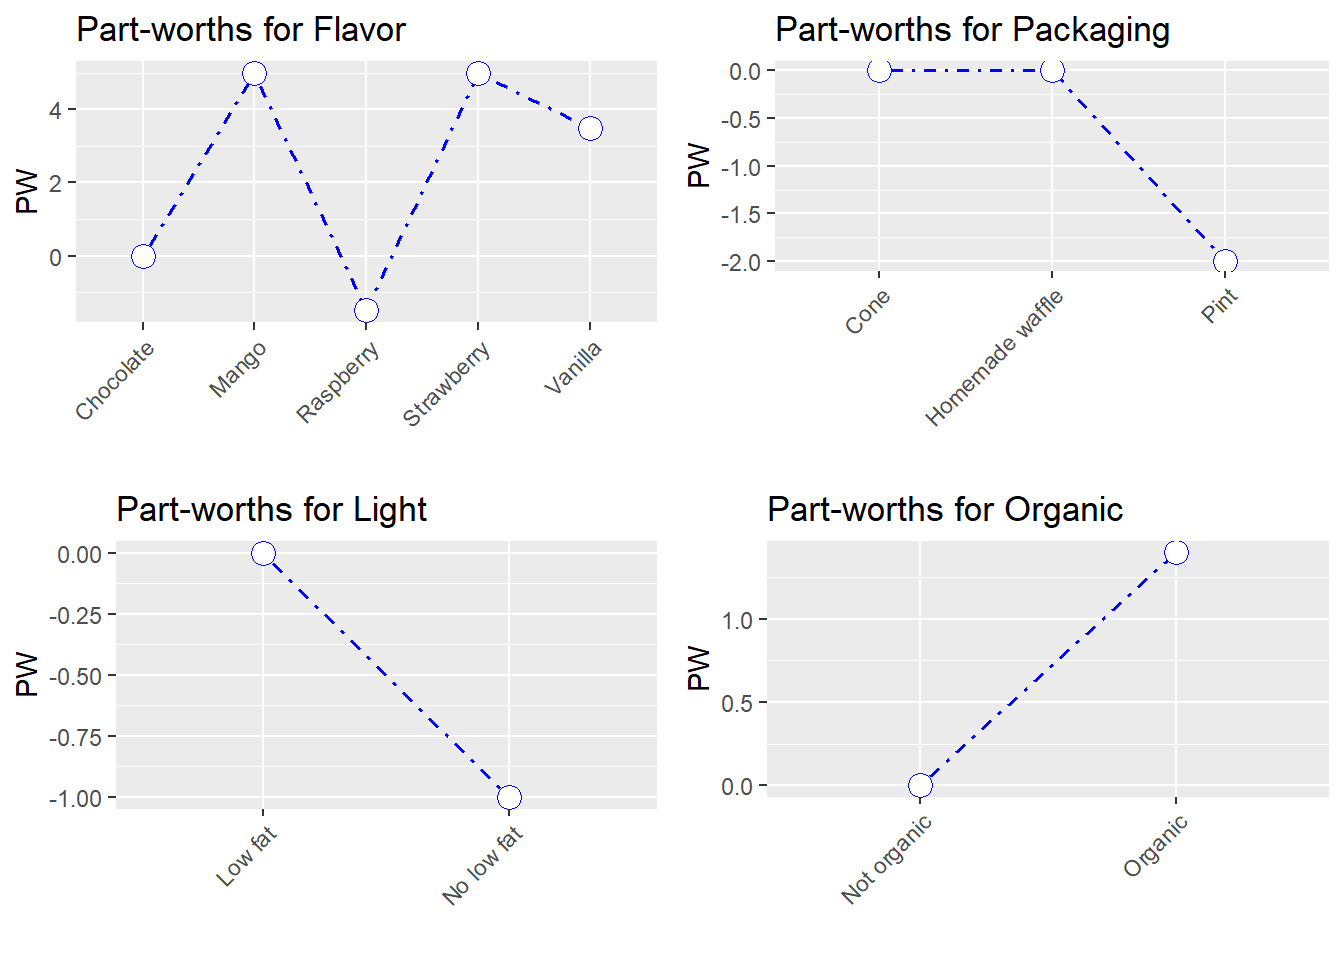
\includegraphics[width=12cm,height=8cm]{conjoint_onerespondent_plot-1.png}
\end{center}

E então vemos facilmente que essa pessoa desfrutaria de um sorvete com baixo teor de gordura, orgânico, manga ou morango em um cone ou em um waffle caseiro.

Observe que os resultados da regressão conjunta são simplesmente os resultados de uma \href{https://bookdown.org/content/1340/linear-regression.html#regression_without}{regressão linear múltipla:}

\begin{lstlisting}[language=R]
# Execute essa regressao se estiver interessado em aprender qual preditor eh significativo ou qual eh o R quadrado do modelo geral.

summary(lm(rating ~ Flavor + Packaging + Light + Organic, data = respondent1))

## 
## Call:
## lm(formula = rating ~ Flavor + Packaging + Light + Organic, data = respondent1)
## 
## Residuals:
##    1    2    3    4    5    6    7    8    9   10 
## -0.3 -0.2  0.3 -0.2  0.2  0.2 -0.3 -0.2  0.2  0.3 
## 
## Coefficients:
##                            Estimate Std. Error t value Pr(>|t|)
## (Intercept)               3.800e+00  8.426e-01   4.510    0.139
## FlavorMango               5.000e+00  9.747e-01   5.130    0.123
## FlavorRaspberry          -1.500e+00  9.747e-01  -1.539    0.367
## FlavorStrawberry          5.000e+00  8.660e-01   5.774    0.109
## FlavorVanilla             3.500e+00  9.747e-01   3.591    0.173
## PackagingHomemade waffle  1.570e-15  8.944e-01   0.000    1.000
## PackagingPint            -2.000e+00  8.660e-01  -2.309    0.260
## LightNo low fat          -1.000e+00  5.916e-01  -1.690    0.340
## OrganicOrganic            1.400e+00  4.899e-01   2.858    0.214
## 
## Residual standard error: 0.7746 on 1 degrees of freedom
## Multiple R-squared:  0.9927, Adjusted R-squared:  0.9345 
## F-statistic: 17.06 on 8 and 1 DF,  p-value: 0.1852
\end{lstlisting}

Finalmente, os pesos de importância nos dizem com que intensidade cada atributo determina a classificação de um sorvete. Para esse respondente, sabor é o atributo mais importante e luz é o atributo menos importante. A classificação deste respondente é determinada em 59,6\% por sabor e em 9,2\% por luz.

\subsubsection{Profiles: utilitários previstos}

Prever as classificações (utilitários) dos diferentes sorvetes é muito fácil em \faRProject. Primeiro, verifique se temos um conjunto de dados com os diferentes perfis que foram testados:

\begin{lstlisting}[language=R]
profiles <- icecream %>% 
  filter(respondent == "Individual 1") %>% 
  select(Flavor,Packaging,Light,Organic)

profiles
## # A tibble: 10 x 4
##    Flavor     Packaging       Light      Organic    
##    <fct>      <fct>           <fct>      <fct>      
##  1 Raspberry  Homemade waffle No low fat Not organic
##  2 Chocolate  Cone            No low fat Organic    
##  3 Raspberry  Pint            Low fat    Organic    
##  4 Strawberry Pint            No low fat Organic    
##  5 Strawberry Cone            Low fat    Not organic
##  6 Chocolate  Homemade waffle No low fat Not organic
##  7 Vanilla    Pint            Low fat    Not organic
##  8 Mango      Homemade waffle Low fat    Organic    
##  9 Mango      Pint            No low fat Not organic
## 10 Vanilla    Homemade waffle No low fat Organic
\end{lstlisting}

Em seguida, pedimos à função \fbox{predict} para prever as classificações dos perfis com base na função de regressão:

\begin{lstlisting}[language=R]
predict(conjoint_respondent1, profiles) # prever as classificacoes para os perfis com base na analise conjunta

## Conjoint Analysis
## Data                 : respondent1 
## Response variable    : rating 
## Explanatory variables: Flavor, Packaging, Light, Organic 
## Prediction dataset   : profiles 
## 
##      Flavor       Packaging      Light     Organic Prediction
##   Raspberry Homemade waffle No low fat Not organic      1.300
##   Chocolate            Cone No low fat     Organic      4.200
##   Raspberry            Pint    Low fat     Organic      1.700
##  Strawberry            Pint No low fat     Organic      7.200
##  Strawberry            Cone    Low fat Not organic      8.800
##   Chocolate Homemade waffle No low fat Not organic      2.800
##     Vanilla            Pint    Low fat Not organic      5.300
##       Mango Homemade waffle    Low fat     Organic     10.200
##       Mango            Pint No low fat Not organic      5.800
##     Vanilla Homemade waffle No low fat     Organic      7.700
\end{lstlisting}

A classificação prevista é mais alta para sorvetes orgânicos com pouca gordura e manga em um waffle caseiro. Mas essas são previsões para sorvetes que o entrevistado realmente classificou. Se quiséssemos saber qual sorvete o entrevistado mais gostava, poderíamos apenas olhar para as classificações observadas (em vez das previstas). É mais interessante obter previsões para sorvetes que o entrevistado não avaliou. Para isso, precisamos dos perfis para todos os sorvetes possíveis. Podemos criar esses perfis com a \fbox{função expand.grid}. A \fbox{função expand.grid} usa dois ou mais vetores e cria todas as combinações possíveis de elementos desses vetores:

\begin{lstlisting}[language=R]
Flavor <- c("Raspberry","Chocolate","Mango","Strawberry","Vanilla")
Organic <- c("Organic","Not organic")

expand.grid(Flavor, Organic)
##          Var1        Var2
## 1   Raspberry     Organic
## 2   Chocolate     Organic
## 3       Mango     Organic
## 4  Strawberry     Organic
## 5     Vanilla     Organic
## 6   Raspberry Not organic
## 7   Chocolate Not organic
## 8       Mango Not organic
## 9  Strawberry Not organic
## 10    Vanilla Not organic
\end{lstlisting}

Vamos fazer isso para todos os nossos níveis de atributo:

\begin{lstlisting}[language=R]
# existe uma maneira mais facil de obter niveis de atributo do que criar os vetores manualmente:

levels(icecream$Flavor) # certifique-se de que o sabor seja fatorado primeiro!

## [1] "Chocolate"  "Mango"      "Raspberry"  "Strawberry" "Vanilla"
# agora crie todos os profiles

profiles.all <- expand.grid(levels(icecream$Flavor),levels(icecream$Packaging),levels(icecream$Light),levels(icecream$Organic)) %>% 
  rename("Flavor" = "Var1", "Packaging" = "Var2", "Light" = "Var3", "Organic" = "Var4") # rename the variables created by expand.grid (don't forget this, otherwise predict won't know where to look for each attribute)

# prever as classificações de todos os perfis

predict(conjoint_respondent1, profiles.all) %>% 
  arrange(desc(Prediction)) # mostrar os sorvetes com a classificação mais alta prevista no topo
  
##        Flavor       Packaging      Light     Organic Prediction
## 1  Strawberry Homemade waffle    Low fat     Organic       10.2
## 2  Strawberry            Cone    Low fat     Organic       10.2
## 3       Mango Homemade waffle    Low fat     Organic       10.2
## 4       Mango            Cone    Low fat     Organic       10.2
## 5  Strawberry Homemade waffle No low fat     Organic        9.2
## 6  Strawberry            Cone No low fat     Organic        9.2
## 7       Mango Homemade waffle No low fat     Organic        9.2
## 8       Mango            Cone No low fat     Organic        9.2
## 9  Strawberry Homemade waffle    Low fat Not organic        8.8
## 10 Strawberry            Cone    Low fat Not organic        8.8
## 11      Mango Homemade waffle    Low fat Not organic        8.8
## 12      Mango            Cone    Low fat Not organic        8.8
## 13    Vanilla Homemade waffle    Low fat     Organic        8.7
## 14    Vanilla            Cone    Low fat     Organic        8.7
## 15 Strawberry            Pint    Low fat     Organic        8.2
## 16      Mango            Pint    Low fat     Organic        8.2
## 17 Strawberry Homemade waffle No low fat Not organic        7.8
## 18 Strawberry            Cone No low fat Not organic        7.8
## 19      Mango Homemade waffle No low fat Not organic        7.8
## 20      Mango            Cone No low fat Not organic        7.8
## 21    Vanilla Homemade waffle No low fat     Organic        7.7
## 22    Vanilla            Cone No low fat     Organic        7.7
## 23    Vanilla Homemade waffle    Low fat Not organic        7.3
## 24    Vanilla            Cone    Low fat Not organic        7.3
## 25 Strawberry            Pint No low fat     Organic        7.2
## 26      Mango            Pint No low fat     Organic        7.2
## 27 Strawberry            Pint    Low fat Not organic        6.8
## 28      Mango            Pint    Low fat Not organic        6.8
## 29    Vanilla            Pint    Low fat     Organic        6.7
## 30    Vanilla Homemade waffle No low fat Not organic        6.3
## 31    Vanilla            Cone No low fat Not organic        6.3
## 32 Strawberry            Pint No low fat Not organic        5.8
## 33      Mango            Pint No low fat Not organic        5.8
## 34    Vanilla            Pint No low fat     Organic        5.7
## 35    Vanilla            Pint    Low fat Not organic        5.3
## 36  Chocolate Homemade waffle    Low fat     Organic        5.2
## 37  Chocolate            Cone    Low fat     Organic        5.2
## 38    Vanilla            Pint No low fat Not organic        4.3
## 39  Chocolate Homemade waffle No low fat     Organic        4.2
## 40  Chocolate            Cone No low fat     Organic        4.2
## 41  Chocolate Homemade waffle    Low fat Not organic        3.8
## 42  Chocolate            Cone    Low fat Not organic        3.8
## 43  Raspberry Homemade waffle    Low fat     Organic        3.7
## 44  Raspberry            Cone    Low fat     Organic        3.7
## 45  Chocolate            Pint    Low fat     Organic        3.2
## 46  Chocolate Homemade waffle No low fat Not organic        2.8
## 47  Chocolate            Cone No low fat Not organic        2.8
## 48  Raspberry Homemade waffle No low fat     Organic        2.7
## 49  Raspberry            Cone No low fat     Organic        2.7
## 50  Raspberry Homemade waffle    Low fat Not organic        2.3
## 51  Raspberry            Cone    Low fat Not organic        2.3
## 52  Chocolate            Pint No low fat     Organic        2.2
## 53  Chocolate            Pint    Low fat Not organic        1.8
## 54  Raspberry            Pint    Low fat     Organic        1.7
## 55  Raspberry Homemade waffle No low fat Not organic        1.3
## 56  Raspberry            Cone No low fat Not organic        1.3
## 57  Chocolate            Pint No low fat Not organic        0.8
## 58  Raspberry            Pint No low fat     Organic        0.7
## 59  Raspberry            Pint    Low fat Not organic        0.3
## 60  Raspberry            Pint No low fat Not organic       -0.7
\end{lstlisting}



Mesma conclusão que a da seção anterior: essa pessoa desfrutaria de um sorvete com baixo teor de gordura, orgânico, manga ou morango em um cone ou um waffle caseiro.

\subsection{Muitos respondentes}

\subsubsection{Estimar valores de peça e pesos de importância}

Agora, vamos realizar a análise conjunta no conjunto de dados completo para ter uma idéia de quais sorvetes os 15 entrevistados, em média, gostaram mais e qual a importância de cada atributo:

\begin{lstlisting}[language=R]
conjoint_allrespondents <- conjoint(icecream, rvar = "rating", evar = c("Flavor","Packaging","Light","Organic")) # como antes, mas com um conjunto de dados diferente.

summary(conjoint_allrespondents) 

## Conjoint analysis
## Data                 : icecream 
## Response variable    : rating 
## Explanatory variables: Flavor, Packaging, Light, Organic 
## 
## Conjoint part-worths:
##    Attributes          Levels     PW
##  Flavor       Chocolate        0.000
##  Flavor       Mango            1.522
##  Flavor       Raspberry        0.522
##  Flavor       Strawberry       0.767
##  Flavor       Vanilla          1.389
##  Packaging    Cone             0.000
##  Packaging    Homemade waffle -0.244
##  Packaging    Pint            -0.100
##  Light        Low fat          0.000
##  Light        No low fat       0.478
##  Organic      Not organic      0.000
##  Organic      Organic          0.307
##  Base utility ~                4.358
## 
## Conjoint importance weights:
##  Attributes    IW
##   Flavor    0.597
##   Packaging 0.096
##   Light     0.187
##   Organic   0.120
## 
## Conjoint regression results:
## 
##                            coefficient
##  (Intercept)                     4.358
##  Flavor|Mango                    1.522
##  Flavor|Raspberry                0.522
##  Flavor|Strawberry               0.767
##  Flavor|Vanilla                  1.389
##  Packaging|Homemade waffle      -0.244
##  Packaging|Pint                 -0.100
##  Light|No low fat                0.478
##  Organic|Organic                 0.307
\end{lstlisting}

O sabor é de longe o atributo mais importante. Vamos traçar estes resultados:

\begin{lstlisting}[language=R]
plot(conjoint_allrespondents)
\end{lstlisting}

\begin{center}
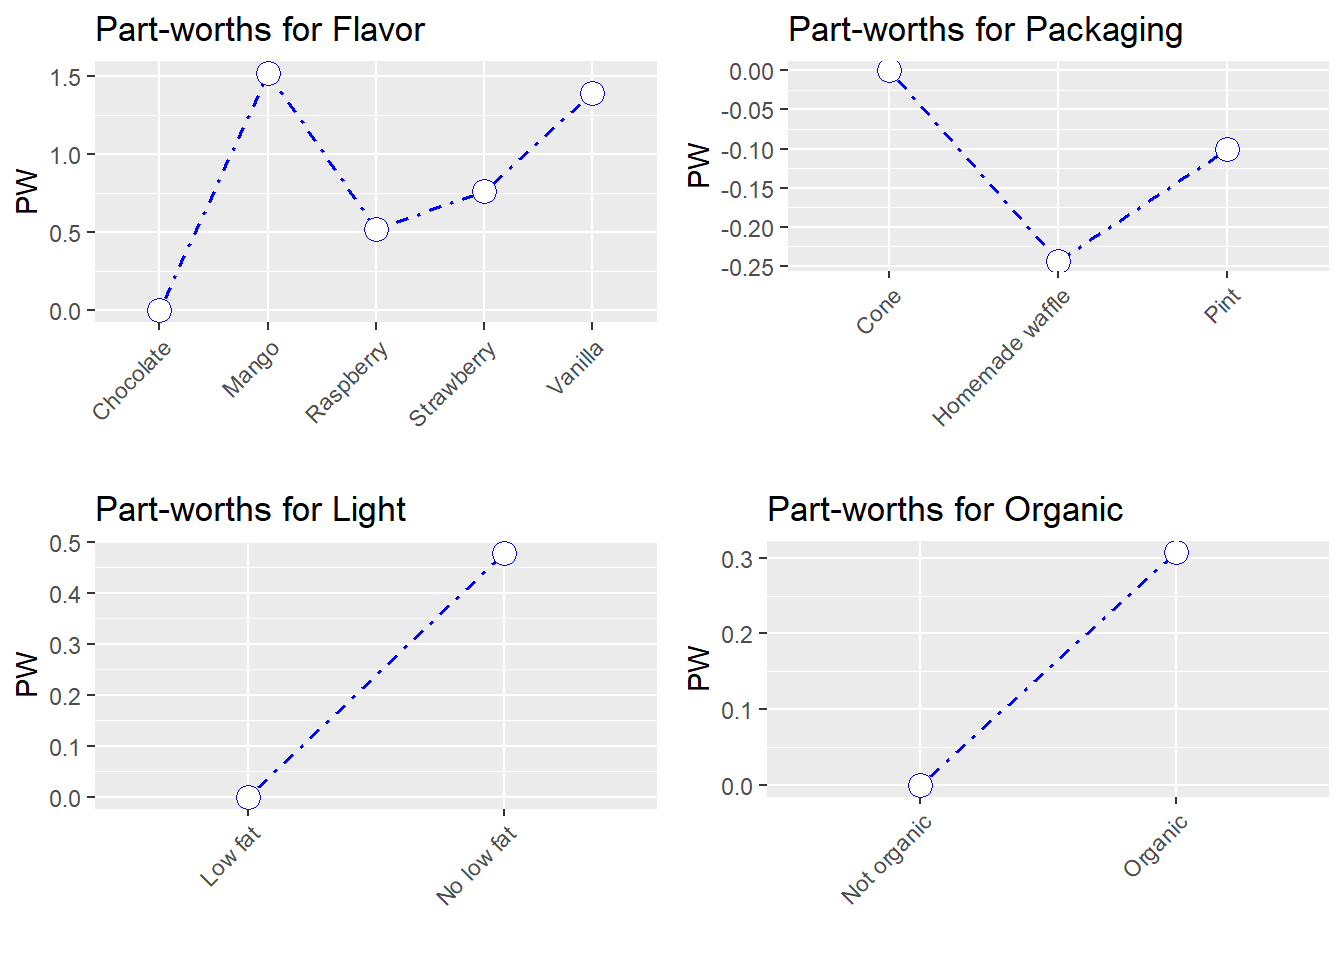
\includegraphics[width=12cm,height=8cm]{conjoint_manyrespondents_plot-1.png}
\end{center}

A partir disso, prevemos que, em média, as pessoas mais gostariam de um sorvete de manga orgânico, sem pouca gordura, em um cone.

Os pesos de importância nos dizem com que intensidade cada atributo determina a classificação média de um sorvete. O sabor é o atributo mais importante e a embalagem é o atributo menos importante. A classificação deste respondente é determinada para 59,7\% por sabor e para 9,6\% por embalagem.

\subsubsection{Profiles: utilitários previstos}

Vamos prever as classificações de todos os sorvetes possíveis:

\begin{lstlisting}[language=R]
predict(conjoint_allrespondents, profiles.all) %>% # verifique as secoes anteriores para profiles.all

  arrange(desc(Prediction)) # mostrar os sorvetes com a classificacao mais alta prevista no topo
  
##        Flavor       Packaging      Light     Organic Prediction
## 1       Mango            Cone No low fat     Organic   6.664444
## 2       Mango            Pint No low fat     Organic   6.564444
## 3     Vanilla            Cone No low fat     Organic   6.531111
## 4     Vanilla            Pint No low fat     Organic   6.431111
## 5       Mango Homemade waffle No low fat     Organic   6.420000
## 6       Mango            Cone No low fat Not organic   6.357778
## 7     Vanilla Homemade waffle No low fat     Organic   6.286667
## 8       Mango            Pint No low fat Not organic   6.257778
## 9     Vanilla            Cone No low fat Not organic   6.224444
## 10      Mango            Cone    Low fat     Organic   6.186667
## 11    Vanilla            Pint No low fat Not organic   6.124444
## 12      Mango Homemade waffle No low fat Not organic   6.113333
## 13      Mango            Pint    Low fat     Organic   6.086667
## 14    Vanilla            Cone    Low fat     Organic   6.053333
## 15    Vanilla Homemade waffle No low fat Not organic   5.980000
## 16    Vanilla            Pint    Low fat     Organic   5.953333
## 17      Mango Homemade waffle    Low fat     Organic   5.942222
## 18 Strawberry            Cone No low fat     Organic   5.908889
## 19      Mango            Cone    Low fat Not organic   5.880000
## 20    Vanilla Homemade waffle    Low fat     Organic   5.808889
## 21 Strawberry            Pint No low fat     Organic   5.808889
## 22      Mango            Pint    Low fat Not organic   5.780000
## 23    Vanilla            Cone    Low fat Not organic   5.746667
## 24  Raspberry            Cone No low fat     Organic   5.664444
## 25 Strawberry Homemade waffle No low fat     Organic   5.664444
## 26    Vanilla            Pint    Low fat Not organic   5.646667
## 27      Mango Homemade waffle    Low fat Not organic   5.635556
## 28 Strawberry            Cone No low fat Not organic   5.602222
## 29  Raspberry            Pint No low fat     Organic   5.564444
## 30    Vanilla Homemade waffle    Low fat Not organic   5.502222
## 31 Strawberry            Pint No low fat Not organic   5.502222
## 32 Strawberry            Cone    Low fat     Organic   5.431111
## 33  Raspberry Homemade waffle No low fat     Organic   5.420000
## 34  Raspberry            Cone No low fat Not organic   5.357778
## 35 Strawberry Homemade waffle No low fat Not organic   5.357778
## 36 Strawberry            Pint    Low fat     Organic   5.331111
## 37  Raspberry            Pint No low fat Not organic   5.257778
## 38  Raspberry            Cone    Low fat     Organic   5.186667
## 39 Strawberry Homemade waffle    Low fat     Organic   5.186667
## 40  Chocolate            Cone No low fat     Organic   5.142222
## 41 Strawberry            Cone    Low fat Not organic   5.124444
## 42  Raspberry Homemade waffle No low fat Not organic   5.113333
## 43  Raspberry            Pint    Low fat     Organic   5.086667
## 44  Chocolate            Pint No low fat     Organic   5.042222
## 45 Strawberry            Pint    Low fat Not organic   5.024444
## 46  Raspberry Homemade waffle    Low fat     Organic   4.942222
## 47  Chocolate Homemade waffle No low fat     Organic   4.897778
## 48  Raspberry            Cone    Low fat Not organic   4.880000
## 49 Strawberry Homemade waffle    Low fat Not organic   4.880000
## 50  Chocolate            Cone No low fat Not organic   4.835556
## 51  Raspberry            Pint    Low fat Not organic   4.780000
## 52  Chocolate            Pint No low fat Not organic   4.735556
## 53  Chocolate            Cone    Low fat     Organic   4.664444
## 54  Raspberry Homemade waffle    Low fat Not organic   4.635556
## 55  Chocolate Homemade waffle No low fat Not organic   4.591111
## 56  Chocolate            Pint    Low fat     Organic   4.564444
## 57  Chocolate Homemade waffle    Low fat     Organic   4.420000
## 58  Chocolate            Cone    Low fat Not organic   4.357778
## 59  Chocolate            Pint    Low fat Not organic   4.257778
## 60  Chocolate Homemade waffle    Low fat Not organic   4.113333
\end{lstlisting}


Mesmas conclusões de antes: prevemos que, em média, as pessoas mais gostariam de um sorvete de manga orgânico, sem pouca gordura, em um cone.

\subsection{Simulação de Mercado}

Digamos que criamos um pequeno número de sorvetes e queremos estimar a participação de mercado de cada um desses sorvetes. Digamos que selecionamos os quatro perfis a seguir:

\begin{lstlisting}[language=R]
# use slice() para selecionar as linhas 

market_profiles <- profiles.all %>% 
  slice(c(4, 16, 23, 38)) # de profiles.all, selecione as linhas 4, 16, 23, 38 como quatro profiles

market_profiles

##       Flavor       Packaging      Light     Organic
## 1 Strawberry            Cone    Low fat Not organic
## 2  Chocolate            Cone No low fat Not organic
## 3  Raspberry Homemade waffle No low fat Not organic
## 4  Raspberry Homemade waffle    Low fat     Organic

#Já sabemos como estimar qual sorvete será mais apreciado:

conjoint_allrespondents <- conjoint(icecream, rvar = "rating", evar = c("Flavor","Packaging","Light","Organic"))

predict(conjoint_allrespondents, market_profiles) %>%
  arrange(desc(Prediction))
  
##       Flavor       Packaging      Light     Organic Prediction
## 1 Strawberry            Cone    Low fat Not organic   5.124444
## 2  Raspberry Homemade waffle No low fat Not organic   5.113333
## 3  Raspberry Homemade waffle    Low fat     Organic   4.942222
## 4  Chocolate            Cone No low fat Not organic   4.835556
\end{lstlisting}

O sorvete de morango com baixo teor de gordura e não orgânico em um cone tem a classificação mais alta prevista entre todos os entrevistados. Mas isso não nos diz qual será a participação de mercado de cada um dos quatro perfis. Para isso, precisamos saber, para cada participante, qual perfil ele escolheria. Em outras palavras, precisamos prever as classificações para cada indivíduo separadamente:

\begin{lstlisting}[language=R]
# mesmo modelo de antes, mas agora adicione por = "respondent"
conjoint_perrespondent <- conjoint(icecream, rvar = "rating", evar = c("Flavor","Packaging","Light","Organic"), by = "respondent")

predict(conjoint_perrespondent, market_profiles) %>% 
  arrange(respondent, desc(Prediction)) # classificar por respondente e depois por classificacao prevista
  
##       respondent     Flavor       Packaging      Light     Organic
## 1   Individual 1 Strawberry            Cone    Low fat Not organic
## 2   Individual 1  Raspberry Homemade waffle    Low fat     Organic
## 3   Individual 1  Chocolate            Cone No low fat Not organic
## 4   Individual 1  Raspberry Homemade waffle No low fat Not organic
## 5  Individual 10  Raspberry Homemade waffle No low fat Not organic
## 6  Individual 10  Raspberry Homemade waffle    Low fat     Organic
## 7  Individual 10  Chocolate            Cone No low fat Not organic
## 8  Individual 10 Strawberry            Cone    Low fat Not organic
## 9  Individual 11 Strawberry            Cone    Low fat Not organic
## 10 Individual 11  Raspberry Homemade waffle    Low fat     Organic
## 11 Individual 11  Chocolate            Cone No low fat Not organic
## 12 Individual 11  Raspberry Homemade waffle No low fat Not organic
## 13 Individual 12  Raspberry Homemade waffle No low fat Not organic
## 14 Individual 12  Raspberry Homemade waffle    Low fat     Organic
## 15 Individual 12  Chocolate            Cone No low fat Not organic
## 16 Individual 12 Strawberry            Cone    Low fat Not organic
## 17 Individual 13  Raspberry Homemade waffle No low fat Not organic
## 18 Individual 13  Raspberry Homemade waffle    Low fat     Organic
## 19 Individual 13  Chocolate            Cone No low fat Not organic
## 20 Individual 13 Strawberry            Cone    Low fat Not organic
## 21 Individual 14  Raspberry Homemade waffle No low fat Not organic
## 22 Individual 14  Raspberry Homemade waffle    Low fat     Organic
## 23 Individual 14 Strawberry            Cone    Low fat Not organic
## 24 Individual 14  Chocolate            Cone No low fat Not organic
## 25 Individual 15 Strawberry            Cone    Low fat Not organic
## 26 Individual 15  Chocolate            Cone No low fat Not organic
## 27 Individual 15  Raspberry Homemade waffle No low fat Not organic
## 28 Individual 15  Raspberry Homemade waffle    Low fat     Organic
## 29  Individual 2 Strawberry            Cone    Low fat Not organic
## 30  Individual 2  Chocolate            Cone No low fat Not organic
## 31  Individual 2  Raspberry Homemade waffle    Low fat     Organic
## 32  Individual 2  Raspberry Homemade waffle No low fat Not organic
## 33  Individual 3  Chocolate            Cone No low fat Not organic
## 34  Individual 3  Raspberry Homemade waffle    Low fat     Organic
## 35  Individual 3  Raspberry Homemade waffle No low fat Not organic
## 36  Individual 3 Strawberry            Cone    Low fat Not organic
## 37  Individual 4  Raspberry Homemade waffle    Low fat     Organic
## 38  Individual 4  Chocolate            Cone No low fat Not organic
## 39  Individual 4 Strawberry            Cone    Low fat Not organic
## 40  Individual 4  Raspberry Homemade waffle No low fat Not organic
## 41  Individual 5 Strawberry            Cone    Low fat Not organic
## 42  Individual 5  Chocolate            Cone No low fat Not organic
## 43  Individual 5  Raspberry Homemade waffle No low fat Not organic
## 44  Individual 5  Raspberry Homemade waffle    Low fat     Organic
## 45  Individual 6  Raspberry Homemade waffle    Low fat     Organic
## 46  Individual 6  Raspberry Homemade waffle No low fat Not organic
## 47  Individual 6  Chocolate            Cone No low fat Not organic
## 48  Individual 6 Strawberry            Cone    Low fat Not organic
## 49  Individual 7 Strawberry            Cone    Low fat Not organic
## 50  Individual 7  Raspberry Homemade waffle No low fat Not organic
## 51  Individual 7  Raspberry Homemade waffle    Low fat     Organic
## 52  Individual 7  Chocolate            Cone No low fat Not organic
## 53  Individual 8  Chocolate            Cone No low fat Not organic
## 54  Individual 8 Strawberry            Cone    Low fat Not organic
## 55  Individual 8  Raspberry Homemade waffle No low fat Not organic
## 56  Individual 8  Raspberry Homemade waffle    Low fat     Organic
## 57  Individual 9 Strawberry            Cone    Low fat Not organic
## 58  Individual 9  Chocolate            Cone No low fat Not organic
## 59  Individual 9  Raspberry Homemade waffle    Low fat     Organic
## 60  Individual 9  Raspberry Homemade waffle No low fat Not organic
##    Prediction
## 1   8.8000000
## 2   3.7000000
## 3   2.8000000
## 4   1.3000000
## 5   9.9500000
## 6   8.9666667
## 7   5.3666667
## 8   2.0333333
## 9   5.8000000
## 10  5.2000000
## 11  3.8000000
## 12  2.8000000
## 13  9.6000000
## 14  7.7333333
## 15  5.9333333
## 16  3.2666667
## 17  6.5500000
## 18  6.2000000
## 19  5.3000000
## 20  1.3000000
## 21  9.8000000
## 22  6.8666667
## 23  5.1333333
## 24  3.4666667
## 25  8.5333333
## 26  6.8666667
## 27  5.7000000
## 28  1.9666667
## 29  9.6333333
## 30  5.9666667
## 31  4.8666667
## 32  3.5500000
## 33  5.5666667
## 34  4.7666667
## 35  4.6500000
## 36  2.2333333
## 37  4.2000000
## 38  3.3000000
## 39  2.3000000
## 40  2.0500000
## 41  4.9333333
## 42  4.2666667
## 43  2.1000000
## 44  2.0666667
## 45  9.4000000
## 46  7.6000000
## 47  2.6000000
## 48  1.6000000
## 49  9.1666667
## 50  6.7500000
## 51  5.3333333
## 52  4.8333333
## 53  4.9333333
## 54  4.2666667
## 55  3.1000000
## 56  0.7333333
## 57  7.8666667
## 58  7.5333333
## 59  2.1333333
## 60  1.2000000
\end{lstlisting}

Vamos reter para cada indivíduo apenas seu perfil mais bem classificado. Podemos fazer isso agrupando por entrevistado e adicionando uma variável denominada ranking que nos dirá o ranking de perfis, com base na classificação prevista, para cada entrevistado:

\begin{lstlisting}[language=R]
highest_rated <- predict(conjoint_perrespondent, market_profiles) %>% 
  group_by(respondent) %>% 
  mutate(ranking = rank(Prediction))

# dando uma olhada
highest_rated %>% 
  arrange(respondent, ranking)
  
## # A tibble: 60 x 7
## # Groups:   respondent [15]
##    respondent   Flavor   Packaging    Light   Organic   Prediction ranking
##    <chr>        <fct>    <fct>        <fct>   <fct>          <dbl>   <dbl>
##  1 Individual 1 Raspber~ Homemade wa~ No low~ Not orga~       1.3        1
##  2 Individual 1 Chocola~ Cone         No low~ Not orga~       2.80       2
##  3 Individual 1 Raspber~ Homemade wa~ Low fat Organic         3.7        3
##  4 Individual 1 Strawbe~ Cone         Low fat Not orga~       8.8        4
##  5 Individual ~ Strawbe~ Cone         Low fat Not orga~       2.03       1
##  6 Individual ~ Chocola~ Cone         No low~ Not orga~       5.37       2
##  7 Individual ~ Raspber~ Homemade wa~ Low fat Organic         8.97       3
##  8 Individual ~ Raspber~ Homemade wa~ No low~ Not orga~       9.95       4
##  9 Individual ~ Raspber~ Homemade wa~ No low~ Not orga~       2.8        1
## 10 Individual ~ Chocola~ Cone         No low~ Not orga~       3.80       2
## # ... with 50 more rows
# precisamos reter apenas o sorvete mais bem classificado

highest_rated <- highest_rated %>% 
  arrange(respondent, ranking) %>% 
  filter(ranking == 4)

highest_rated

## # A tibble: 15 x 7
## # Groups:   respondent [15]
##    respondent   Flavor   Packaging    Light   Organic   Prediction ranking
##    <chr>        <fct>    <fct>        <fct>   <fct>          <dbl>   <dbl>
##  1 Individual 1 Strawbe~ Cone         Low fat Not orga~       8.8        4
##  2 Individual ~ Raspber~ Homemade wa~ No low~ Not orga~       9.95       4
##  3 Individual ~ Strawbe~ Cone         Low fat Not orga~       5.80       4
##  4 Individual ~ Raspber~ Homemade wa~ No low~ Not orga~       9.60       4
##  5 Individual ~ Raspber~ Homemade wa~ No low~ Not orga~       6.55       4
##  6 Individual ~ Raspber~ Homemade wa~ No low~ Not orga~       9.8        4
##  7 Individual ~ Strawbe~ Cone         Low fat Not orga~       8.53       4
##  8 Individual 2 Strawbe~ Cone         Low fat Not orga~       9.63       4
##  9 Individual 3 Chocola~ Cone         No low~ Not orga~       5.57       4
## 10 Individual 4 Raspber~ Homemade wa~ Low fat Organic         4.2        4
## 11 Individual 5 Strawbe~ Cone         Low fat Not orga~       4.93       4
## 12 Individual 6 Raspber~ Homemade wa~ Low fat Organic         9.40       4
## 13 Individual 7 Strawbe~ Cone         Low fat Not orga~       9.17       4
## 14 Individual 8 Chocola~ Cone         No low~ Not orga~       4.93       4
## 15 Individual 9 Strawbe~ Cone         Low fat Not orga~       7.87       4
\end{lstlisting}



Agora podemos estimar a participação de mercado:

\begin{lstlisting}[language=R]
market_share <- highest_rated %>% 
  group_by(Flavor, Packaging, Light, Organic) %>% 
  summarize(count = n()) %>% 
  arrange(desc(count))

market_share

## # A tibble: 4 x 5
## # Groups:   Flavor, Packaging, Light [4]
##   Flavor     Packaging       Light      Organic     count
##   <fct>      <fct>           <fct>      <fct>       <int>
## 1 Strawberry Cone            Low fat    Not organic     7
## 2 Raspberry  Homemade waffle No low fat Not organic     4
## 3 Chocolate  Cone            No low fat Not organic     2
## 4 Raspberry  Homemade waffle Low fat    Organic         2
\end{lstlisting}


Vimos que o sorvete de morango, cone, baixo teor de gordura e não orgânico é preferido por 7 em cada 15 participantes, o framboesa, waffle caseiro, sem baixo teor de gordura e sorvete não orgânico é favorecido por 4 em cada 15 participantes e assim por diante .



%======================================================
\newpage
%=====================================================

\begin{thebibliography}{99}
\bibitem{rformarketingstudents} \textbf{\faRProject for Marketing Students.} Disponível em: \href{https://bookdown.org/content/1340/}{https://bookdown.org/content/1340/} 

\bibitem{overleaf} \textbf{Overleaf, online \LaTeX~ editor}. Disponível em \href{http://www.overleaf.com}{Overleaf.com} 

\bibitem{xie} Xie, Y. \textbf{Dynamic Documents with \faRProject and knitr} 2nd edition, 2015.

\bibitem{JARick} \textbf{Reproducible Research using \faRMarkdown and Overleaf.} Disponível em \href{https://static1.squarespace.com/static/5757268f7da24f26ca7b21d2/t/5c7587114192021796d7cc84/1551206162093/R_Overleaf_Integration.pdf}{Reproducible Research using RMarkdown and Overleaf}
\end{thebibliography}










%===================================================
\end{document}